\documentclass[12pt,a4paper]{article}
\usepackage{apacite}
\usepackage{graphicx}
%\usepackage[top=4cm, bottom=4cm, outer=5cm, inner=3cm, heightrounded, marginparwidth=3cm, marginparsep=1cm]{geometry} %TODO: comment out
%\usepackage[marginparwidth=2.5cm, marginparsep=2cm]{geometry}
\usepackage[toc,page]{appendix}
\usepackage{hyperref}
\usepackage{fancyref}
\usepackage[round]{natbib}
\usepackage{fancyhdr}
\usepackage{setspace}
\usepackage{pgf}
\usepackage{color, colortbl}
\usepackage{float}
\usepackage{capt-of}
%\usepackage[justification=centering]{caption}
\pagestyle{fancy}

\newcommand{\citetwo}[4]{(\citeauthor{#1}, \citeyear{#1}, p.~#2; \citeauthor{#3}, \citeyear{#3}, p.~#4)}

\newcommand{\HRule}{\rule{\linewidth}{0.5mm}}

\definecolor{Gray}{gray}{0.9}



\begin{document}

\begin{titlepage}

\begin{center}

\textsc{\LARGE University of Edinburgh}\\[1cm]

\textsc{\Large Dissertation in Language Sciences}\\[1.5cm]

\HRule \\[0.4cm]
{ \huge \bfseries Understanding Referential Coordination as a Particle Swarm Optimization Task \\[0.4cm] }

\HRule \\[1.5cm]


\noindent
\begin{minipage}{0.4\textwidth}
\begin{flushleft} \large
\emph{Exam Number:}\\
\textsc{B018520}
\end{flushleft}
\end{minipage}%
\begin{minipage}{0.4\textwidth}
\begin{flushright} \large
\emph{Supervisor:} \\
Dr.~Hannah \textsc{Rohde}
\end{flushright}
\end{minipage}

\vfill

% Bottom of the page
{\large 1st April, 2015}
%\title{Understanding Referential Coordination as a Particle Swarm Optimization Task}
%\author{s1107496}
%\date{1st April, 2015}

%\maketitle

\end{center}
\end{titlepage}

%\onehalfspace
\doublespace

\begin{abstract}
The question of how referential choice and interpretation are influenced by production cost remains unresolved in the literature. A recent paper \citep{rohde2012} investigates the conditions under which speakers choose to coordinate using low-cost but ambiguous expressions by conducting a number of experiments in which participants played an iterated referential coordination language game. This dissertation takes a novel approach to modeling referential coordination by simulating \citeauthor{rohde2012}'s results using particle swarm optimization (PSO), a general-purpose optimization method for non-differentiable problems with continuous search spaces. Two PSO-based models are presented, one of which is shown to perform well against a baseline model. Predictions from the more favourable of the two models are presented for several variants of the \citeauthor{rohde2012} language games, extrapolating from the results of the original studies. This model is also shown to partially replicate observed findings of persistent entrainment on lexical forms, even when a changing discourse context causes these forms to become overinformative \citep{brennan1996}. The results from the PSO model are taken to demonstrate that dyadic referential coordination can be framed as a constrained optimization problem in which agents do not need to maintain an explicit representation of the common ground or of each other - a finding in keeping with egocentric accounts of communication from the literature \citep{horton1996}.
\end{abstract}

\pagebreak


\tableofcontents

\pagebreak


\section{Introduction}
An open question in the field of linguistics is how participants in a conversation coordinate their use of referring expressions. When producing referring expressions, interlocutors must weigh the costs they incur when producing the expression, in terms of both construction and articulation, against the ease with which their conversational partners will be able to infer the intended referent. When speakers employ referring expressions that do not uniquely select a referent within the context of the discourse, they further risk their conversational partner failing to infer the correct referent. For example, consider a discourse context in which there are three plausible referents, a chocolate Labrador, a black Poodle, and a brown American Water Spaniel/German Longhaired Pointer mix. Given the high cost of producing an unambiguous referring expression for the latter, a speaker might attempt to refer to the American Water Spaniel/German Longhaired Pointer mix as ``that brown dog". However, this expression could also plausibly be used to indicate the chocolate Labrador, and should the speaker's communicative partner interpret the referring expression as such, rectifying this misinterpretation is likely to be costly. While communicating, interlocutors therefore jointly seek to minimize their expended effort while not violating the constraint imposed by their partner's ability to disambiguate the referring expressions used \citep[p.~65-66]{benz2005}. Consequently, the referential strategy a speaker adopts must be sensitive to the relative costs of producing each reference as well as the evolving state of mappings between referential form and intended referent, as coordinated with their interlocutors. 

Recent work has employed the use of language games to investigate how speakers make selections from a given set of available ambiguous and unambiguous referring expressions (\citeauthor{rohde2012} \citeyear{rohde2012}; \citeauthor{degen2012} \citeyear{degen2012}; \citeauthor{frank2012} \citeyear{frank2012}). Unlike some studies which have targeted one-time production choices, \citeauthor{rohde2012}'s studies notably involve both human speakers and comprehenders, and test the coordination of referring expressions in a "conversational" (multiple turn) scenario. To do so, \citeauthor{rohde2012} introduced an iterated language game in which participant dyads were rewarded for coordinating their use of ambiguous and unambiguous referring expressions. In these studies, participants' ability to successfully coordinate on the use of less costly ambiguous forms was shown to be affected by the relative costs of the available competing unambiguous forms. This paper seeks to introduce a computational model of \citeauthor{rohde2012}'s findings, and, in doing so, consider how modeling may be applied to the problem of referential coordination. Such a model would allow simulation of the experimentally infeasible or impossible, as well as enabling extrapolation from the data collected in the lab, the results of which can be used to drive further studies in potentially fruitful directions. Further to this, computational models in general uniquely allow for direct inspection of their parameters and processes, which can shed light on aspects of human cognition. As such, computational modeling has seen extensive use in the field of linguistics, notable examples including the use of iterated learning to demonstrate the spontaneous construction of optimal lexicons \citep{smith2002} and spontaneous emergence of syntax \citep{kirby2002}, the use of incremental probabilistic parsing to model garden-path sentence comprehension \citep{hale2001}, and the use of Bayesian statistics to model referential inference \citep{frank2012}.

When selecting a modeling approach for \cite{rohde2012}, three crucial considerations must be taken into account: first, the chosen approach needs to represent the internal state of a participant with respect to the game, and to allow the participant's actions to be derived from this state; second, changes in a participant's internal state within the model need to be reflective of the participant's communicative success with their partner, even as their partner's internal state itself changes; and third, the modeling approach should be easily extensible to many variants of the \citeauthor{rohde2012} language games. Particle swarm optimization is suitable in all three regards. Originally introduced by \citet*{kennedy1995}, particle swarm optimization (PSO) can serve not only as a general optimization method, but also as a means of modeling human social behaviour, especially in the context of collaborative problem solving \citep{kennedy1997}. These factors make the technique an ideal candidate for modeling referential communication. 

A particle-swarm-based model would allow a more exhaustive exploration of the effects of various form costs on referential coordination, offering a comprehensive picture of the circumstances under which ambiguous form entrainment is possible and likely. Further to this, an accurate particle-swarm-based model of human coordination in a discourse setting might shed light on more fundamental aspects of human cognition and social interaction as represented by the model's parameters. A successful model could also suggest PSO's suitability for the modeling of other linguistic phenomena. 

Conversely, if PSO is not a viable means of modeling the results observed in \citeauthor{rohde2012}, this could suggest a fundamental difference between human linguistic behaviours and other social behaviours successfully modeled via PSO. A negative finding might also suggest that specialized methods are required to model more complex human social interactions.

To address these possibilities, this paper models \citeauthor{rohde2012}'s experiments as a PSO task, utilizing a mixed strategy search space to represent form production and comprehension. Two model variants optimized to the \citeauthor{rohde2012} language games are presented, which differ in their treatment of the search space; one of these models is shown to compare favorably to a baseline PSO model. Both models respond to changes in form costs in a promisingly similar fashion to the observed experimental data, although neither perfectly replicates human trials.


\section{Background}
\subsection{Referential coordination}
\subsubsection{Overview}
Language is an inherently cooperative endeavour. To successfully understand and be understood by their interlocutors, speakers must actively coordinate their use of referring expressions, and rely on their communicative partners to do the same. The mechanisms by which this coordination can occur with relative facility are an active topic of research, and of special interest is the extent to which speakers maintain internal models of their interlocutors in order to inform their communicative strategies. Research has also been devoted to the processes by which speakers balance the costs they incur when communicating against those incurred by their interlocutors, and how the interplay of these combined factors directs the evolution of referential mappings during discourse. While certain communication games have been analyzed within a game-theoretic framework (e.g. \citeauthor{rohde2012} \citeyear{rohde2012}, \citeauthor{degen2012} \citeyear{degen2012}), the psycholinguistics literature has largely approached the topic of referential coordination from the perspective of audience design; this section therefore provides an overview of previous work done in both communities.

\subsubsection{Game theoretic approaches}
Game theory provides a methodology for understanding agents' actions by modeling them as strategies within games. When deciding on which actions to choose, agents are said to attempt to maximize their expected utility by leveraging their knowledge of the game's state \citep{benz2005}. As applied to linguistics, game theoretic concepts can be used to describe a number of phenomena; for instance, \cite{jaeger2008} demonstrates how an evolutionary game-theoretic framework (in which systematic stability is maximized) can be successfully applied to the division of the vowel space in order to predict the vowel systems of modern-day languages.

\cite{lewis1969} established much of the foundation necessary to frame language in game-theoretic terms, namely, providing an account of the establishment of conventions as a coordinative (this is to say, positive-sum) game in which agents' interests are aligned. His work has been built upon in order to apply game theory to the more specific problem of referential coordination. For example, by convention, the use of more general but costly referring expressions implicitly excludes the referents of easily accessed and more specific forms (e.g. ``cutter" versus ``knife", or ``some" versus ``all"). The establishment of this convention has been explained using an evolutionary (but ontogenetic) game-theoretic approach: both speaker and hearer benefit from an interpretation of the former which carries a greater degree of information (e.g. ``cutters which are not knives", ``some but not all") \citep{benz2005}. More recent work by \cite{degen2012} has used game theoretic models to predict participant behaviour in referential inference tasks with some success, although the researchers expressed the need for more nuanced, comprehensive models (an example of which this paper attempts to provide). 

\subsubsection{Psycholinguistic approaches}
The problem of referential coordination within the psycholinguistics literature has primarily been framed in terms of audience design. According to one school of thought, as presented in \cite{clark1982}, speakers carefully tailor utterances to best target their specific interlocutor or interlocutors; likewise, listeners interpret the meaning of utterances with respect not only to the speaker but, it is claimed, with respect to the speaker's presumed beliefs about the listener as well. Under this model, audience design on the speaker's part enables the listener to disambiguate the referent of an otherwise ambiguous referring expression, provided the listener's internal model of the speaker suffices to allow the listener to understand why the speaker has chosen that particular referring expression. 

As an example (adapted from \citeauthor{clark1982}), suppose Alice and Bob are conversing; Alice mentions to Bob something about ``your friend". Given the reasonable assumption that Bob has more than one friend, the referent of this expression is ambiguous. However, if Alice has met only one of Bob's friends, she may rely on him to recognize this fact and interpret the expression accordingly. From Bob's perspective, to disambiguate Alice's referring expression, he must both recall that Alice has met only one of his friends and  correctly reason that she will expect him to recall this (and to leverage this information to infer a referent). As interlocutors, over the course of a discourse or number of discourses, update and maintain their models of each other and the common information shared between them, they become increasingly entrained on specific lexical forms which are reflective of this shared knowledge and experience.

This understanding of referential coordination is borne out in work on natural language generation. For example, \cite{golland2010} utilize a game-theoretic approach to realize a language game in which an artificial speaker agent must successfully communicate a specified referent to their human listener partner. Their results show that when this artificial speaker is endowed with an internally embedded model of the listener, it is able to substantially outperform simpler models which do not take the listener into account.

While this research makes the implicit assumption that the common ground between speaker and hearer informs production immediately when an utterance is initially being planned, more egocentric models of communication offer a competing view \citep{horton1996}. In a human behavioural study in which participants were required to quickly produce referring expressions for their communicative partners, it was found that time pressure caused the participants to disrespect the common ground more frequently than when speed of production was not encouraged. This was taken to support the conclusion that the common ground does not inform initial utterance planning, but instead is taken into consideration as a filtering mechanism during later-stage utterance production. Furthermore, \citeauthor{horton1996} posited that the common ground may play no role whatsoever in the production of the majority of utterances, citing the potential costliness of routinely taking this information into consideration.

\subsubsection{Rohde et al. 2012}
In ``Communicating with Cost-based Implicature: a Game-Theoretic Approach to Ambiguity" \citeyearpar{rohde2012}, \citeauthor{rohde2012} present an iterated language game in which participants aim to indicate an object to their partner via use of one of several possible referring terms. Participants gain points upon successful communication, but must spend points in order to communicate. Each referent has a corresponding unambiguous form that players may choose to send to their partners; alternatively, players may send an ambiguous form with a different cost that could potentially indicate a number of referents. Players who attain a certain score are allowed to exit the experiment upon doing so, and are in this way incentivized to use the least costly possible expressions to achieve the highest rate of communicative success. Two studies were conducted; in both, two groups of three unambiguous referring expressions were paired with a single less costly ambiguous referring expression which could plausibly be used for any item within the group (see Table \ref{table:rohde}). 

The studies conducted by \citeauthor{rohde2012} demonstrate that the likelihood of a pair of participants successfully coordinating their use of an ambiguous reference is partially contingent on the relative costs of the unambiguous and ambiguous referring expressions. Specifically, pairs of participants were more likely to coordinate on using the ambiguous form in the second study, in which unambiguous form costs were both lower and more similar to each other. This was notably not in keeping with game-theoretic predictions; \citeauthor{rohde2012} suggested that the lower stakes (i.e. more moderate penalties) in the second study resulted in a greater willingness on the part of the participants to explore a wider range of referential strategies. The question that this dissertation asks is whether this behaviour can be better understood as an emergent property of a simulation, such as a PSO-based model.

\begin{table}
\begin{center}
    \begin{tabular}{ c r r }
    & \multicolumn{2}{ c }{Cost} \\ 
    Name & Study 1 & Study 2 \\ \hline
    ``Rose"   & $60$  & $80$ \\ \hline
    ``Daisy"  & $120$ & $140$ \\ \hline
    ``Tulip"  & $280$ & $165$ \\ \hline
    \rowcolor{Gray}
    ``Flower" & $80$  & $80$ \\ \hline
    ``Apple Tree" & $60$  & $80$ \\ \hline
    ``Pine Tree"  & $120$ & $135$ \\ \hline
    ``Palm Tree"  & $250$ & $170$ \\ \hline
    \rowcolor{Gray}
    ``Tree"       & $80$  & $80$ \\ 
    \end{tabular}
    \caption{Referring expression costs used in the \citeauthor{rohde2012} studies, with ambiguous referring expressions highlighted in grey.}
    \label{table:rohde}
\end{center}
\end{table}


\subsection{Particle swarm optimization}
\subsubsection{Overview}
Particle swarm optimization was first formulated by \cite{kennedy1995} in an attempt to model human social behaviour. The initial model was based on \cite{heppner1990}'s work in modeling bird flocking and roosting behaviour in two-dimensional space, refined to allow for an arbitrary number of dimensions and for particles to share the same or arbitrarily close positions within said multidimensional space. \citeauthor{kennedy1995} demonstrated that their new optimization method was suitable not only for use in modeling human social behaviour, but also for the general-purpose optimization of non-linear continuous problems. Specifically, PSO was found to be successful both in optimizing the weights of an artificial neural network and in the Schaffer $f6$ problem, a standard benchmark for general-purpose optimization methods \citep{davis1991}.

The concept behind the PSO algorithm is relatively simple. Potential solutions to some problem with $n$ dimensions are represented as particles existing within an $n$-dimensional search space. Each particle has both a position within this space and some velocity vector. Each particle also keeps track of the best position it has been in as evaluated by the given objective function, which is known as its ``personal" best position; a ``global" best position representing the best position found by any particle within a swarm or swarm subgroup is also maintained \citep{chong2013}. A PSO task is run iteratively, until some stopping criterion is reached \citep{solnon2010}. Every iteration begins by updating the velocities of all particles. In doing so, a particle is acted upon by two forces: the attraction of the particle to its personal previous best known position, as governed by a ``cognitive" parameter, and its attraction to the best known position within its group, as governed by a ``social" parameter \citep{chong2013}. The particle also maintains some momentum from its previous velocity. Following this, particle positions are updated in accordance with their velocities, with new positions being evaluated via the given objective function and best-known personal and global positions updated where appropriate. Initial particle velocities are assigned randomly; in doing so, exploration of the search space is encouraged, reducing the likelihood of the swarm as a whole becoming caught in a local extremum or local extrema of the objective function (\citeauthor{yang2014} \citeyear{yang2014}; \citeauthor{solnon2010} \citeyear{solnon2010}). 

As noted by \citet*{yang2014}, PSO is applicable to a large domain of problems, has straightforward conceptual groundings, and is simple to implement; these factors have spurred on its widespread use in a number of fields, and resulted in the development of numerous refinements and derivatives of the original algorithm. This paper uses the well-known inertial variant of PSO, which offers a ``noticeable improvement" in speedy convergence on good solutions as compared to standard PSO \citep{yang2014}. Further to this variant, for the purposes of this paper, each particle's position is updated with respect to the best-found solution within a predefined neighborhood or group of particles, as opposed to the global best-found solution, as presented in \citet*{solnon2010}. When these particle groups do not intersect, this is simply equivalent to running a number of independent PSO tasks equal to the number of groups.

% mention velocity clamping...? Engelbrecht 109 and in others


\subsubsection{Previous work}
\label{sec:pso_prev_work}

While PSO has been applied to a number of problems within the fields of linguistics and psychology, its primary use has been as a means of optimizing parameters for other models, as opposed to direct application as a model in and of itself (e.g. \citeauthor{chatterjee2005} \citeyear{chatterjee2005}; \citeauthor{mehdad2009} \citeyear{mehdad2009}). Notable exceptions to this trend include the use of PSO to perform unsupervised phoneme clustering \citep{ahmadi2007} and the modeling of human emergency evacuation behaviours via PSO \citep{cheng2008}.

PSO has likewise been applied to game learning, often using a coevolutionary paradigm in which agents play against one another in order to evaluate their fitness. However, traditionally this method has involved PSO over a search space of neural network weights, where the neural networks are used to choose actions given a game state, or in cases where the ``game" is a classical constraint optimization problem, such as the $n$-queens problem \citep[p.~349-351]{engelbrecht2005}. By contrast, in the new approach presented in this paper, the positions of particles themselves comprise agents' internal states, which directly define a mixed strategy (see \autoref{sec:search_space}).  

\subsubsection{Formulation and parameters}
\label{sec:2.2.3}
In the formulation of PSO employed in this paper, a particle $i$ with position $x_i$ has a velocity $v_i$ at time $t$ such that
\begin{equation}
v_i^t = \theta(t) \cdot v_i^{t-1} + \alpha \cdot \epsilon_1 \cdot (x_{N(i)}^* - x_i^{t-1}) + \beta \cdot \epsilon_2 \cdot (x_i^* - x_i^{t-1})
\end{equation}
where $\theta$ is the inertial scheduling function, $\alpha$ is the cognitive component, $\beta$ is the social component, $x_{N(i)}^*$ is the global best position known for $i$'s neighborhood or group $N(i)$, $x_i^*$ is $i$'s personal best known position, and $\epsilon_1$ and $\epsilon_2$ are randomly chosen values within $\left(0.0, 1.0\right]$. Although $\theta$ can take many forms including, most commonly, a constant function \citep{yang2014}, for the purposes of this paper $\theta$ is defined with respect to a base inertia $\tau$ and inertial dampening factor $\sigma$ such that
\begin{equation}
\theta(t) = \frac{\tau}{\sigma^t} 
\end{equation}
Finally, the position $x$ of $i$ at time $t$ is defined as
\begin{equation}
x_i^t = x_i^{t-1} + \phi \cdot v_i^t 
\end{equation}
where $\phi$ is a constant velocity dampening factor.

\section{Methods}

\subsection{Overview}

To model referential coordination within the \citeauthor{rohde2012} language game as a PSO task, individual participants were modeled as particles in groups of size $2$. In exploring the search space of possible game strategies, each particle sought to maximize its score within the language game in relation to the strategy of its partner. The scoring function of the language game itself was parameterized on the relative costs of unambiguous forms, as in \citeauthor{rohde2012}. Further to this, the parameters of the PSO algorithm (cognitive component, social component, etc.) were optimized to best replicate \citeauthor{rohde2012}'s experimental findings. Two models were ultimately produced,\footnote{The full source code for this project is available online at \url{http://git.io/pb5S}.} which differed in their handling of the search space; both were evaluated against the experimental data.

\subsection{Models}
\subsubsection{Search space}
\label{sec:search_space}

In modeling the \citeauthor{rohde2012} language game as a PSO task, the form a solution to the game takes must be considered in order to establish a search space.  To do so, the game-theoretic notion of a mixed strategy was adopted, in which each possible action $a$ within a game is performed by a participant $i$ with some probability $P_i(a)$ \citep{benz2005}. For the given language game, for each referent $r$ the participant can be said to maintain a probability of using the associated ambiguous form $A$, $P_i(A|r)$. Conversely, the probability of a participant using the available unambiguous form for $r$ can be given as $1 - P_i(A|r)$. Therefore, in an instance of the \citeauthor{rohde2012} language game with $n$ possible referents, a participant's strategy was represented with $n$ independent probabilities, yielding an $n$-dimensional search space. 

It is important to note that this does not constitute a traditional mixed strategy, in that a participant's strategy is not a probability distribution. This is to say, the sum of a participant's probability of using the ambiguous referring expression over all referents may not equal $1$. As an example, given two referents $r_1$ and $r_2$, a participant is capable of opting to use the ambiguous form for neither. In this sense, it may be more accurate to state that a participant $i$ maintains a separate mixed strategy for each referent $r$, where, for the ambiguous form $A$ and unambiguous form $U$, $P_i(A|r) + P_i(U|r) = 1$.

It is also important to note that for the purposes of this paper, participants were assumed to optimize their strategies for groups of referents sharing the same ambiguous form independently of other groups.\footnote{In \citeauthor{rohde2012} specifically, the flower category and tree category (see Table \ref{table:rohde}).} As such, the two studies presented in \citeauthor{rohde2012} were each treated as two independent language games being run concurrently, and the PSO approach presented used 3-dimensional search spaces as opposed to 6-dimensional search spaces. This assumption was justified by the observation that participant pairs in \citeauthor{rohde2012}'s second study were able to coordinate their use of the ambiguous form for one group, but not the other. 

Finally, because each dimension in the search space defined above reflects a probability, values outside the interval $[0, 1]$ are invalid. A number of approaches for adapting PSO to constrained optimization problems have been suggested in the literature;\footnote{See \cite{helwig2010} for a recent overview.} two plausible alternatives as presented in \cite{engelbrecht2005} were considered, resulting in two competing models. 
In the first model, particles which moved outside the desired search space immediately had a repair method applied to them, whereby they were relocated to the nearest point which did not violate the given constraints. This model will be referred to as the ``repair" model. In the second model, particles were allowed to move freely within the search space, including to regions that violated constraints. However, particles not meeting the given constraints were allowed to update neither their personal best known position nor the global best position. Because all personal best positions and the global best position therefore remained in feasible space, particles were naturally attracted back to the region of the search space which respected the constraints. The model utilizing this technique will be referred to as the ``rejection" model. In both models, initial particle positions were assigned randomly within the valid search space.


 
\subsubsection{Objective function}
\label{sec:objective_func}
In applying PSO to the \citeauthor{rohde2012} language game, an appropriate representation of the game's goals must be formulated as an objective function. In the game as presented, the expected number of points awarded to participant $i$ given their partner $j$ when asked to communicate referent $r$ can be calculated as follows:\footnote{N.B. that while the notation $P(x|y)$ is normally used solely to indicate the conditional probability of $x$ given $y$, this notation is here additionally used to indicate that $EP_i$ must be evaluated with regards to $i$'s partner $j$, notated as $EP_{i}(r|j)$.}
\begin{equation}
EP_{i}(r|j) = P_i(A|r)(S \cdot P_j(r|A) - cost_A) \,+\, (1 - P_i(A|r))(S - cost_r) 
\end{equation}
where $cost_A$ is the cost of production of the ambiguous form, $S$ is the number of points awarded on successful communication (set at 80 and 85 in \citeauthor{rohde2012}, respectively), and $cost_r$ is the cost of production of the unambiguous form for $r$.

Each round, the actual number of points awarded to participants is dependent on samples from $P_i$ and $P_j$, as well as the randomly-chosen $r$. As such, without the strategies of $i$ or $j$ changing, there are for any given round a number of possible scores $i$ might attain. Relying on the game unmodified as the objective function for a PSO task would therefore be imprudent, as an inconsistent objective function would be much harder to optimize. Instead, the objective function $f$ used for both models was chosen as 
\begin{equation}
f(i) = \sum_{r \in R} EP_{i}(r|j) + EP_{j}(r|i)
\end{equation}

\begin{figure}
\centering
%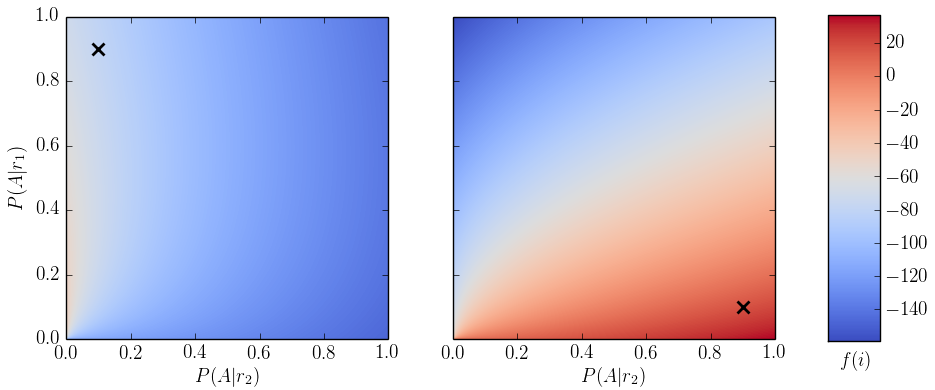
\includegraphics[width=\textwidth]{objective_function_cropped.png}
\scalebox{.725}{%% Creator: Matplotlib, PGF backend
%%
%% To include the figure in your LaTeX document, write
%%   \input{<filename>.pgf}
%%
%% Make sure the required packages are loaded in your preamble
%%   \usepackage{pgf}
%%
%% Figures using additional raster images can only be included by \input if
%% they are in the same directory as the main LaTeX file. For loading figures
%% from other directories you can use the `import` package
%%   \usepackage{import}
%% and then include the figures with
%%   \import{<path to file>}{<filename>.pgf}
%%
%% Matplotlib used the following preamble
%%   \usepackage{fontspec}
%%   \setmainfont{DejaVu Serif}
%%   \setsansfont{DejaVu Sans}
%%   \setmonofont{DejaVu Sans Mono}
%%
\begingroup%
\makeatletter%
\begin{pgfpicture}%
\pgfpathrectangle{\pgfpointorigin}{\pgfqpoint{7.300000in}{4.075000in}}%
\pgfusepath{use as bounding box}%
\begin{pgfscope}%
\pgfsetbuttcap%
\pgfsetroundjoin%
\definecolor{currentfill}{rgb}{1.000000,1.000000,1.000000}%
\pgfsetfillcolor{currentfill}%
\pgfsetlinewidth{0.000000pt}%
\definecolor{currentstroke}{rgb}{1.000000,1.000000,1.000000}%
\pgfsetstrokecolor{currentstroke}%
\pgfsetdash{}{0pt}%
\pgfpathmoveto{\pgfqpoint{0.000000in}{0.000000in}}%
\pgfpathlineto{\pgfqpoint{7.300000in}{0.000000in}}%
\pgfpathlineto{\pgfqpoint{7.300000in}{4.075000in}}%
\pgfpathlineto{\pgfqpoint{0.000000in}{4.075000in}}%
\pgfpathclose%
\pgfusepath{fill}%
\end{pgfscope}%
\begin{pgfscope}%
\pgfsetbuttcap%
\pgfsetroundjoin%
\definecolor{currentfill}{rgb}{1.000000,1.000000,1.000000}%
\pgfsetfillcolor{currentfill}%
\pgfsetlinewidth{0.000000pt}%
\definecolor{currentstroke}{rgb}{0.000000,0.000000,0.000000}%
\pgfsetstrokecolor{currentstroke}%
\pgfsetstrokeopacity{0.000000}%
\pgfsetdash{}{0pt}%
\pgfpathmoveto{\pgfqpoint{0.619395in}{0.804260in}}%
\pgfpathlineto{\pgfqpoint{3.085874in}{0.804260in}}%
\pgfpathlineto{\pgfqpoint{3.085874in}{3.270740in}}%
\pgfpathlineto{\pgfqpoint{0.619395in}{3.270740in}}%
\pgfpathclose%
\pgfusepath{fill}%
\end{pgfscope}%
\begin{pgfscope}%
\pgfpathrectangle{\pgfqpoint{0.619395in}{0.804260in}}{\pgfqpoint{2.466479in}{2.466479in}} %
\pgfusepath{clip}%
\pgftext[at=\pgfqpoint{0.619395in}{0.804260in},left,bottom]{\pgfimage[interpolate=true,width=2.480000in,height=2.480000in]{objective_function-img0.png}}%
\end{pgfscope}%
\begin{pgfscope}%
\pgfpathrectangle{\pgfqpoint{0.619395in}{0.804260in}}{\pgfqpoint{2.466479in}{2.466479in}} %
\pgfusepath{clip}%
\pgfsetrectcap%
\pgfsetroundjoin%
\pgfsetlinewidth{1.003750pt}%
\definecolor{currentstroke}{rgb}{0.000000,0.000000,0.000000}%
\pgfsetstrokecolor{currentstroke}%
\pgfsetdash{}{0pt}%
\pgfpathmoveto{\pgfqpoint{0.866043in}{3.024092in}}%
\pgfusepath{stroke}%
\end{pgfscope}%
\begin{pgfscope}%
\pgfpathrectangle{\pgfqpoint{0.619395in}{0.804260in}}{\pgfqpoint{2.466479in}{2.466479in}} %
\pgfusepath{clip}%
\pgfsetbuttcap%
\pgfsetroundjoin%
\definecolor{currentfill}{rgb}{0.000000,0.000000,0.000000}%
\pgfsetfillcolor{currentfill}%
\pgfsetlinewidth{2.007500pt}%
\definecolor{currentstroke}{rgb}{0.000000,0.000000,0.000000}%
\pgfsetstrokecolor{currentstroke}%
\pgfsetdash{}{0pt}%
\pgfsys@defobject{currentmarker}{\pgfqpoint{-0.055556in}{-0.055556in}}{\pgfqpoint{0.055556in}{0.055556in}}{%
\pgfpathmoveto{\pgfqpoint{-0.055556in}{-0.055556in}}%
\pgfpathlineto{\pgfqpoint{0.055556in}{0.055556in}}%
\pgfpathmoveto{\pgfqpoint{-0.055556in}{0.055556in}}%
\pgfpathlineto{\pgfqpoint{0.055556in}{-0.055556in}}%
\pgfusepath{stroke,fill}%
}%
\begin{pgfscope}%
\pgfsys@transformshift{0.866043in}{3.024092in}%
\pgfsys@useobject{currentmarker}{}%
\end{pgfscope}%
\end{pgfscope}%
\begin{pgfscope}%
\pgfsetbuttcap%
\pgfsetroundjoin%
\definecolor{currentfill}{rgb}{0.000000,0.000000,0.000000}%
\pgfsetfillcolor{currentfill}%
\pgfsetlinewidth{0.501875pt}%
\definecolor{currentstroke}{rgb}{0.000000,0.000000,0.000000}%
\pgfsetstrokecolor{currentstroke}%
\pgfsetdash{}{0pt}%
\pgfsys@defobject{currentmarker}{\pgfqpoint{0.000000in}{0.000000in}}{\pgfqpoint{0.000000in}{0.055556in}}{%
\pgfpathmoveto{\pgfqpoint{0.000000in}{0.000000in}}%
\pgfpathlineto{\pgfqpoint{0.000000in}{0.055556in}}%
\pgfusepath{stroke,fill}%
}%
\begin{pgfscope}%
\pgfsys@transformshift{0.619395in}{0.804260in}%
\pgfsys@useobject{currentmarker}{}%
\end{pgfscope}%
\end{pgfscope}%
\begin{pgfscope}%
\pgfsetbuttcap%
\pgfsetroundjoin%
\definecolor{currentfill}{rgb}{0.000000,0.000000,0.000000}%
\pgfsetfillcolor{currentfill}%
\pgfsetlinewidth{0.501875pt}%
\definecolor{currentstroke}{rgb}{0.000000,0.000000,0.000000}%
\pgfsetstrokecolor{currentstroke}%
\pgfsetdash{}{0pt}%
\pgfsys@defobject{currentmarker}{\pgfqpoint{0.000000in}{-0.055556in}}{\pgfqpoint{0.000000in}{0.000000in}}{%
\pgfpathmoveto{\pgfqpoint{0.000000in}{0.000000in}}%
\pgfpathlineto{\pgfqpoint{0.000000in}{-0.055556in}}%
\pgfusepath{stroke,fill}%
}%
\begin{pgfscope}%
\pgfsys@transformshift{0.619395in}{3.270740in}%
\pgfsys@useobject{currentmarker}{}%
\end{pgfscope}%
\end{pgfscope}%
\begin{pgfscope}%
\pgftext[x=0.619395in,y=0.748705in,,top]{{\sffamily\fontsize{12.000000}{14.400000}\selectfont \(\displaystyle 0.0\)}}%
\end{pgfscope}%
\begin{pgfscope}%
\pgfsetbuttcap%
\pgfsetroundjoin%
\definecolor{currentfill}{rgb}{0.000000,0.000000,0.000000}%
\pgfsetfillcolor{currentfill}%
\pgfsetlinewidth{0.501875pt}%
\definecolor{currentstroke}{rgb}{0.000000,0.000000,0.000000}%
\pgfsetstrokecolor{currentstroke}%
\pgfsetdash{}{0pt}%
\pgfsys@defobject{currentmarker}{\pgfqpoint{0.000000in}{0.000000in}}{\pgfqpoint{0.000000in}{0.055556in}}{%
\pgfpathmoveto{\pgfqpoint{0.000000in}{0.000000in}}%
\pgfpathlineto{\pgfqpoint{0.000000in}{0.055556in}}%
\pgfusepath{stroke,fill}%
}%
\begin{pgfscope}%
\pgfsys@transformshift{1.112691in}{0.804260in}%
\pgfsys@useobject{currentmarker}{}%
\end{pgfscope}%
\end{pgfscope}%
\begin{pgfscope}%
\pgfsetbuttcap%
\pgfsetroundjoin%
\definecolor{currentfill}{rgb}{0.000000,0.000000,0.000000}%
\pgfsetfillcolor{currentfill}%
\pgfsetlinewidth{0.501875pt}%
\definecolor{currentstroke}{rgb}{0.000000,0.000000,0.000000}%
\pgfsetstrokecolor{currentstroke}%
\pgfsetdash{}{0pt}%
\pgfsys@defobject{currentmarker}{\pgfqpoint{0.000000in}{-0.055556in}}{\pgfqpoint{0.000000in}{0.000000in}}{%
\pgfpathmoveto{\pgfqpoint{0.000000in}{0.000000in}}%
\pgfpathlineto{\pgfqpoint{0.000000in}{-0.055556in}}%
\pgfusepath{stroke,fill}%
}%
\begin{pgfscope}%
\pgfsys@transformshift{1.112691in}{3.270740in}%
\pgfsys@useobject{currentmarker}{}%
\end{pgfscope}%
\end{pgfscope}%
\begin{pgfscope}%
\pgftext[x=1.112691in,y=0.748705in,,top]{{\sffamily\fontsize{12.000000}{14.400000}\selectfont \(\displaystyle 0.2\)}}%
\end{pgfscope}%
\begin{pgfscope}%
\pgfsetbuttcap%
\pgfsetroundjoin%
\definecolor{currentfill}{rgb}{0.000000,0.000000,0.000000}%
\pgfsetfillcolor{currentfill}%
\pgfsetlinewidth{0.501875pt}%
\definecolor{currentstroke}{rgb}{0.000000,0.000000,0.000000}%
\pgfsetstrokecolor{currentstroke}%
\pgfsetdash{}{0pt}%
\pgfsys@defobject{currentmarker}{\pgfqpoint{0.000000in}{0.000000in}}{\pgfqpoint{0.000000in}{0.055556in}}{%
\pgfpathmoveto{\pgfqpoint{0.000000in}{0.000000in}}%
\pgfpathlineto{\pgfqpoint{0.000000in}{0.055556in}}%
\pgfusepath{stroke,fill}%
}%
\begin{pgfscope}%
\pgfsys@transformshift{1.605987in}{0.804260in}%
\pgfsys@useobject{currentmarker}{}%
\end{pgfscope}%
\end{pgfscope}%
\begin{pgfscope}%
\pgfsetbuttcap%
\pgfsetroundjoin%
\definecolor{currentfill}{rgb}{0.000000,0.000000,0.000000}%
\pgfsetfillcolor{currentfill}%
\pgfsetlinewidth{0.501875pt}%
\definecolor{currentstroke}{rgb}{0.000000,0.000000,0.000000}%
\pgfsetstrokecolor{currentstroke}%
\pgfsetdash{}{0pt}%
\pgfsys@defobject{currentmarker}{\pgfqpoint{0.000000in}{-0.055556in}}{\pgfqpoint{0.000000in}{0.000000in}}{%
\pgfpathmoveto{\pgfqpoint{0.000000in}{0.000000in}}%
\pgfpathlineto{\pgfqpoint{0.000000in}{-0.055556in}}%
\pgfusepath{stroke,fill}%
}%
\begin{pgfscope}%
\pgfsys@transformshift{1.605987in}{3.270740in}%
\pgfsys@useobject{currentmarker}{}%
\end{pgfscope}%
\end{pgfscope}%
\begin{pgfscope}%
\pgftext[x=1.605987in,y=0.748705in,,top]{{\sffamily\fontsize{12.000000}{14.400000}\selectfont \(\displaystyle 0.4\)}}%
\end{pgfscope}%
\begin{pgfscope}%
\pgfsetbuttcap%
\pgfsetroundjoin%
\definecolor{currentfill}{rgb}{0.000000,0.000000,0.000000}%
\pgfsetfillcolor{currentfill}%
\pgfsetlinewidth{0.501875pt}%
\definecolor{currentstroke}{rgb}{0.000000,0.000000,0.000000}%
\pgfsetstrokecolor{currentstroke}%
\pgfsetdash{}{0pt}%
\pgfsys@defobject{currentmarker}{\pgfqpoint{0.000000in}{0.000000in}}{\pgfqpoint{0.000000in}{0.055556in}}{%
\pgfpathmoveto{\pgfqpoint{0.000000in}{0.000000in}}%
\pgfpathlineto{\pgfqpoint{0.000000in}{0.055556in}}%
\pgfusepath{stroke,fill}%
}%
\begin{pgfscope}%
\pgfsys@transformshift{2.099283in}{0.804260in}%
\pgfsys@useobject{currentmarker}{}%
\end{pgfscope}%
\end{pgfscope}%
\begin{pgfscope}%
\pgfsetbuttcap%
\pgfsetroundjoin%
\definecolor{currentfill}{rgb}{0.000000,0.000000,0.000000}%
\pgfsetfillcolor{currentfill}%
\pgfsetlinewidth{0.501875pt}%
\definecolor{currentstroke}{rgb}{0.000000,0.000000,0.000000}%
\pgfsetstrokecolor{currentstroke}%
\pgfsetdash{}{0pt}%
\pgfsys@defobject{currentmarker}{\pgfqpoint{0.000000in}{-0.055556in}}{\pgfqpoint{0.000000in}{0.000000in}}{%
\pgfpathmoveto{\pgfqpoint{0.000000in}{0.000000in}}%
\pgfpathlineto{\pgfqpoint{0.000000in}{-0.055556in}}%
\pgfusepath{stroke,fill}%
}%
\begin{pgfscope}%
\pgfsys@transformshift{2.099283in}{3.270740in}%
\pgfsys@useobject{currentmarker}{}%
\end{pgfscope}%
\end{pgfscope}%
\begin{pgfscope}%
\pgftext[x=2.099283in,y=0.748705in,,top]{{\sffamily\fontsize{12.000000}{14.400000}\selectfont \(\displaystyle 0.6\)}}%
\end{pgfscope}%
\begin{pgfscope}%
\pgfsetbuttcap%
\pgfsetroundjoin%
\definecolor{currentfill}{rgb}{0.000000,0.000000,0.000000}%
\pgfsetfillcolor{currentfill}%
\pgfsetlinewidth{0.501875pt}%
\definecolor{currentstroke}{rgb}{0.000000,0.000000,0.000000}%
\pgfsetstrokecolor{currentstroke}%
\pgfsetdash{}{0pt}%
\pgfsys@defobject{currentmarker}{\pgfqpoint{0.000000in}{0.000000in}}{\pgfqpoint{0.000000in}{0.055556in}}{%
\pgfpathmoveto{\pgfqpoint{0.000000in}{0.000000in}}%
\pgfpathlineto{\pgfqpoint{0.000000in}{0.055556in}}%
\pgfusepath{stroke,fill}%
}%
\begin{pgfscope}%
\pgfsys@transformshift{2.592579in}{0.804260in}%
\pgfsys@useobject{currentmarker}{}%
\end{pgfscope}%
\end{pgfscope}%
\begin{pgfscope}%
\pgfsetbuttcap%
\pgfsetroundjoin%
\definecolor{currentfill}{rgb}{0.000000,0.000000,0.000000}%
\pgfsetfillcolor{currentfill}%
\pgfsetlinewidth{0.501875pt}%
\definecolor{currentstroke}{rgb}{0.000000,0.000000,0.000000}%
\pgfsetstrokecolor{currentstroke}%
\pgfsetdash{}{0pt}%
\pgfsys@defobject{currentmarker}{\pgfqpoint{0.000000in}{-0.055556in}}{\pgfqpoint{0.000000in}{0.000000in}}{%
\pgfpathmoveto{\pgfqpoint{0.000000in}{0.000000in}}%
\pgfpathlineto{\pgfqpoint{0.000000in}{-0.055556in}}%
\pgfusepath{stroke,fill}%
}%
\begin{pgfscope}%
\pgfsys@transformshift{2.592579in}{3.270740in}%
\pgfsys@useobject{currentmarker}{}%
\end{pgfscope}%
\end{pgfscope}%
\begin{pgfscope}%
\pgftext[x=2.592579in,y=0.748705in,,top]{{\sffamily\fontsize{12.000000}{14.400000}\selectfont \(\displaystyle 0.8\)}}%
\end{pgfscope}%
\begin{pgfscope}%
\pgfsetbuttcap%
\pgfsetroundjoin%
\definecolor{currentfill}{rgb}{0.000000,0.000000,0.000000}%
\pgfsetfillcolor{currentfill}%
\pgfsetlinewidth{0.501875pt}%
\definecolor{currentstroke}{rgb}{0.000000,0.000000,0.000000}%
\pgfsetstrokecolor{currentstroke}%
\pgfsetdash{}{0pt}%
\pgfsys@defobject{currentmarker}{\pgfqpoint{0.000000in}{0.000000in}}{\pgfqpoint{0.000000in}{0.055556in}}{%
\pgfpathmoveto{\pgfqpoint{0.000000in}{0.000000in}}%
\pgfpathlineto{\pgfqpoint{0.000000in}{0.055556in}}%
\pgfusepath{stroke,fill}%
}%
\begin{pgfscope}%
\pgfsys@transformshift{3.085874in}{0.804260in}%
\pgfsys@useobject{currentmarker}{}%
\end{pgfscope}%
\end{pgfscope}%
\begin{pgfscope}%
\pgfsetbuttcap%
\pgfsetroundjoin%
\definecolor{currentfill}{rgb}{0.000000,0.000000,0.000000}%
\pgfsetfillcolor{currentfill}%
\pgfsetlinewidth{0.501875pt}%
\definecolor{currentstroke}{rgb}{0.000000,0.000000,0.000000}%
\pgfsetstrokecolor{currentstroke}%
\pgfsetdash{}{0pt}%
\pgfsys@defobject{currentmarker}{\pgfqpoint{0.000000in}{-0.055556in}}{\pgfqpoint{0.000000in}{0.000000in}}{%
\pgfpathmoveto{\pgfqpoint{0.000000in}{0.000000in}}%
\pgfpathlineto{\pgfqpoint{0.000000in}{-0.055556in}}%
\pgfusepath{stroke,fill}%
}%
\begin{pgfscope}%
\pgfsys@transformshift{3.085874in}{3.270740in}%
\pgfsys@useobject{currentmarker}{}%
\end{pgfscope}%
\end{pgfscope}%
\begin{pgfscope}%
\pgftext[x=3.085874in,y=0.748705in,,top]{{\sffamily\fontsize{12.000000}{14.400000}\selectfont \(\displaystyle 1.0\)}}%
\end{pgfscope}%
\begin{pgfscope}%
\pgftext[x=1.852635in,y=0.517965in,,top]{{\sffamily\fontsize{12.000000}{14.400000}\selectfont \(\displaystyle P(A|r_2)\)}}%
\end{pgfscope}%
\begin{pgfscope}%
\pgfsetbuttcap%
\pgfsetroundjoin%
\definecolor{currentfill}{rgb}{0.000000,0.000000,0.000000}%
\pgfsetfillcolor{currentfill}%
\pgfsetlinewidth{0.501875pt}%
\definecolor{currentstroke}{rgb}{0.000000,0.000000,0.000000}%
\pgfsetstrokecolor{currentstroke}%
\pgfsetdash{}{0pt}%
\pgfsys@defobject{currentmarker}{\pgfqpoint{0.000000in}{0.000000in}}{\pgfqpoint{0.055556in}{0.000000in}}{%
\pgfpathmoveto{\pgfqpoint{0.000000in}{0.000000in}}%
\pgfpathlineto{\pgfqpoint{0.055556in}{0.000000in}}%
\pgfusepath{stroke,fill}%
}%
\begin{pgfscope}%
\pgfsys@transformshift{0.619395in}{0.804260in}%
\pgfsys@useobject{currentmarker}{}%
\end{pgfscope}%
\end{pgfscope}%
\begin{pgfscope}%
\pgfsetbuttcap%
\pgfsetroundjoin%
\definecolor{currentfill}{rgb}{0.000000,0.000000,0.000000}%
\pgfsetfillcolor{currentfill}%
\pgfsetlinewidth{0.501875pt}%
\definecolor{currentstroke}{rgb}{0.000000,0.000000,0.000000}%
\pgfsetstrokecolor{currentstroke}%
\pgfsetdash{}{0pt}%
\pgfsys@defobject{currentmarker}{\pgfqpoint{-0.055556in}{0.000000in}}{\pgfqpoint{0.000000in}{0.000000in}}{%
\pgfpathmoveto{\pgfqpoint{0.000000in}{0.000000in}}%
\pgfpathlineto{\pgfqpoint{-0.055556in}{0.000000in}}%
\pgfusepath{stroke,fill}%
}%
\begin{pgfscope}%
\pgfsys@transformshift{3.085874in}{0.804260in}%
\pgfsys@useobject{currentmarker}{}%
\end{pgfscope}%
\end{pgfscope}%
\begin{pgfscope}%
\pgftext[x=0.563839in,y=0.804260in,right,]{{\sffamily\fontsize{12.000000}{14.400000}\selectfont \(\displaystyle 0.0\)}}%
\end{pgfscope}%
\begin{pgfscope}%
\pgfsetbuttcap%
\pgfsetroundjoin%
\definecolor{currentfill}{rgb}{0.000000,0.000000,0.000000}%
\pgfsetfillcolor{currentfill}%
\pgfsetlinewidth{0.501875pt}%
\definecolor{currentstroke}{rgb}{0.000000,0.000000,0.000000}%
\pgfsetstrokecolor{currentstroke}%
\pgfsetdash{}{0pt}%
\pgfsys@defobject{currentmarker}{\pgfqpoint{0.000000in}{0.000000in}}{\pgfqpoint{0.055556in}{0.000000in}}{%
\pgfpathmoveto{\pgfqpoint{0.000000in}{0.000000in}}%
\pgfpathlineto{\pgfqpoint{0.055556in}{0.000000in}}%
\pgfusepath{stroke,fill}%
}%
\begin{pgfscope}%
\pgfsys@transformshift{0.619395in}{1.297556in}%
\pgfsys@useobject{currentmarker}{}%
\end{pgfscope}%
\end{pgfscope}%
\begin{pgfscope}%
\pgfsetbuttcap%
\pgfsetroundjoin%
\definecolor{currentfill}{rgb}{0.000000,0.000000,0.000000}%
\pgfsetfillcolor{currentfill}%
\pgfsetlinewidth{0.501875pt}%
\definecolor{currentstroke}{rgb}{0.000000,0.000000,0.000000}%
\pgfsetstrokecolor{currentstroke}%
\pgfsetdash{}{0pt}%
\pgfsys@defobject{currentmarker}{\pgfqpoint{-0.055556in}{0.000000in}}{\pgfqpoint{0.000000in}{0.000000in}}{%
\pgfpathmoveto{\pgfqpoint{0.000000in}{0.000000in}}%
\pgfpathlineto{\pgfqpoint{-0.055556in}{0.000000in}}%
\pgfusepath{stroke,fill}%
}%
\begin{pgfscope}%
\pgfsys@transformshift{3.085874in}{1.297556in}%
\pgfsys@useobject{currentmarker}{}%
\end{pgfscope}%
\end{pgfscope}%
\begin{pgfscope}%
\pgftext[x=0.563839in,y=1.297556in,right,]{{\sffamily\fontsize{12.000000}{14.400000}\selectfont \(\displaystyle 0.2\)}}%
\end{pgfscope}%
\begin{pgfscope}%
\pgfsetbuttcap%
\pgfsetroundjoin%
\definecolor{currentfill}{rgb}{0.000000,0.000000,0.000000}%
\pgfsetfillcolor{currentfill}%
\pgfsetlinewidth{0.501875pt}%
\definecolor{currentstroke}{rgb}{0.000000,0.000000,0.000000}%
\pgfsetstrokecolor{currentstroke}%
\pgfsetdash{}{0pt}%
\pgfsys@defobject{currentmarker}{\pgfqpoint{0.000000in}{0.000000in}}{\pgfqpoint{0.055556in}{0.000000in}}{%
\pgfpathmoveto{\pgfqpoint{0.000000in}{0.000000in}}%
\pgfpathlineto{\pgfqpoint{0.055556in}{0.000000in}}%
\pgfusepath{stroke,fill}%
}%
\begin{pgfscope}%
\pgfsys@transformshift{0.619395in}{1.790852in}%
\pgfsys@useobject{currentmarker}{}%
\end{pgfscope}%
\end{pgfscope}%
\begin{pgfscope}%
\pgfsetbuttcap%
\pgfsetroundjoin%
\definecolor{currentfill}{rgb}{0.000000,0.000000,0.000000}%
\pgfsetfillcolor{currentfill}%
\pgfsetlinewidth{0.501875pt}%
\definecolor{currentstroke}{rgb}{0.000000,0.000000,0.000000}%
\pgfsetstrokecolor{currentstroke}%
\pgfsetdash{}{0pt}%
\pgfsys@defobject{currentmarker}{\pgfqpoint{-0.055556in}{0.000000in}}{\pgfqpoint{0.000000in}{0.000000in}}{%
\pgfpathmoveto{\pgfqpoint{0.000000in}{0.000000in}}%
\pgfpathlineto{\pgfqpoint{-0.055556in}{0.000000in}}%
\pgfusepath{stroke,fill}%
}%
\begin{pgfscope}%
\pgfsys@transformshift{3.085874in}{1.790852in}%
\pgfsys@useobject{currentmarker}{}%
\end{pgfscope}%
\end{pgfscope}%
\begin{pgfscope}%
\pgftext[x=0.563839in,y=1.790852in,right,]{{\sffamily\fontsize{12.000000}{14.400000}\selectfont \(\displaystyle 0.4\)}}%
\end{pgfscope}%
\begin{pgfscope}%
\pgfsetbuttcap%
\pgfsetroundjoin%
\definecolor{currentfill}{rgb}{0.000000,0.000000,0.000000}%
\pgfsetfillcolor{currentfill}%
\pgfsetlinewidth{0.501875pt}%
\definecolor{currentstroke}{rgb}{0.000000,0.000000,0.000000}%
\pgfsetstrokecolor{currentstroke}%
\pgfsetdash{}{0pt}%
\pgfsys@defobject{currentmarker}{\pgfqpoint{0.000000in}{0.000000in}}{\pgfqpoint{0.055556in}{0.000000in}}{%
\pgfpathmoveto{\pgfqpoint{0.000000in}{0.000000in}}%
\pgfpathlineto{\pgfqpoint{0.055556in}{0.000000in}}%
\pgfusepath{stroke,fill}%
}%
\begin{pgfscope}%
\pgfsys@transformshift{0.619395in}{2.284148in}%
\pgfsys@useobject{currentmarker}{}%
\end{pgfscope}%
\end{pgfscope}%
\begin{pgfscope}%
\pgfsetbuttcap%
\pgfsetroundjoin%
\definecolor{currentfill}{rgb}{0.000000,0.000000,0.000000}%
\pgfsetfillcolor{currentfill}%
\pgfsetlinewidth{0.501875pt}%
\definecolor{currentstroke}{rgb}{0.000000,0.000000,0.000000}%
\pgfsetstrokecolor{currentstroke}%
\pgfsetdash{}{0pt}%
\pgfsys@defobject{currentmarker}{\pgfqpoint{-0.055556in}{0.000000in}}{\pgfqpoint{0.000000in}{0.000000in}}{%
\pgfpathmoveto{\pgfqpoint{0.000000in}{0.000000in}}%
\pgfpathlineto{\pgfqpoint{-0.055556in}{0.000000in}}%
\pgfusepath{stroke,fill}%
}%
\begin{pgfscope}%
\pgfsys@transformshift{3.085874in}{2.284148in}%
\pgfsys@useobject{currentmarker}{}%
\end{pgfscope}%
\end{pgfscope}%
\begin{pgfscope}%
\pgftext[x=0.563839in,y=2.284148in,right,]{{\sffamily\fontsize{12.000000}{14.400000}\selectfont \(\displaystyle 0.6\)}}%
\end{pgfscope}%
\begin{pgfscope}%
\pgfsetbuttcap%
\pgfsetroundjoin%
\definecolor{currentfill}{rgb}{0.000000,0.000000,0.000000}%
\pgfsetfillcolor{currentfill}%
\pgfsetlinewidth{0.501875pt}%
\definecolor{currentstroke}{rgb}{0.000000,0.000000,0.000000}%
\pgfsetstrokecolor{currentstroke}%
\pgfsetdash{}{0pt}%
\pgfsys@defobject{currentmarker}{\pgfqpoint{0.000000in}{0.000000in}}{\pgfqpoint{0.055556in}{0.000000in}}{%
\pgfpathmoveto{\pgfqpoint{0.000000in}{0.000000in}}%
\pgfpathlineto{\pgfqpoint{0.055556in}{0.000000in}}%
\pgfusepath{stroke,fill}%
}%
\begin{pgfscope}%
\pgfsys@transformshift{0.619395in}{2.777444in}%
\pgfsys@useobject{currentmarker}{}%
\end{pgfscope}%
\end{pgfscope}%
\begin{pgfscope}%
\pgfsetbuttcap%
\pgfsetroundjoin%
\definecolor{currentfill}{rgb}{0.000000,0.000000,0.000000}%
\pgfsetfillcolor{currentfill}%
\pgfsetlinewidth{0.501875pt}%
\definecolor{currentstroke}{rgb}{0.000000,0.000000,0.000000}%
\pgfsetstrokecolor{currentstroke}%
\pgfsetdash{}{0pt}%
\pgfsys@defobject{currentmarker}{\pgfqpoint{-0.055556in}{0.000000in}}{\pgfqpoint{0.000000in}{0.000000in}}{%
\pgfpathmoveto{\pgfqpoint{0.000000in}{0.000000in}}%
\pgfpathlineto{\pgfqpoint{-0.055556in}{0.000000in}}%
\pgfusepath{stroke,fill}%
}%
\begin{pgfscope}%
\pgfsys@transformshift{3.085874in}{2.777444in}%
\pgfsys@useobject{currentmarker}{}%
\end{pgfscope}%
\end{pgfscope}%
\begin{pgfscope}%
\pgftext[x=0.563839in,y=2.777444in,right,]{{\sffamily\fontsize{12.000000}{14.400000}\selectfont \(\displaystyle 0.8\)}}%
\end{pgfscope}%
\begin{pgfscope}%
\pgfsetbuttcap%
\pgfsetroundjoin%
\definecolor{currentfill}{rgb}{0.000000,0.000000,0.000000}%
\pgfsetfillcolor{currentfill}%
\pgfsetlinewidth{0.501875pt}%
\definecolor{currentstroke}{rgb}{0.000000,0.000000,0.000000}%
\pgfsetstrokecolor{currentstroke}%
\pgfsetdash{}{0pt}%
\pgfsys@defobject{currentmarker}{\pgfqpoint{0.000000in}{0.000000in}}{\pgfqpoint{0.055556in}{0.000000in}}{%
\pgfpathmoveto{\pgfqpoint{0.000000in}{0.000000in}}%
\pgfpathlineto{\pgfqpoint{0.055556in}{0.000000in}}%
\pgfusepath{stroke,fill}%
}%
\begin{pgfscope}%
\pgfsys@transformshift{0.619395in}{3.270740in}%
\pgfsys@useobject{currentmarker}{}%
\end{pgfscope}%
\end{pgfscope}%
\begin{pgfscope}%
\pgfsetbuttcap%
\pgfsetroundjoin%
\definecolor{currentfill}{rgb}{0.000000,0.000000,0.000000}%
\pgfsetfillcolor{currentfill}%
\pgfsetlinewidth{0.501875pt}%
\definecolor{currentstroke}{rgb}{0.000000,0.000000,0.000000}%
\pgfsetstrokecolor{currentstroke}%
\pgfsetdash{}{0pt}%
\pgfsys@defobject{currentmarker}{\pgfqpoint{-0.055556in}{0.000000in}}{\pgfqpoint{0.000000in}{0.000000in}}{%
\pgfpathmoveto{\pgfqpoint{0.000000in}{0.000000in}}%
\pgfpathlineto{\pgfqpoint{-0.055556in}{0.000000in}}%
\pgfusepath{stroke,fill}%
}%
\begin{pgfscope}%
\pgfsys@transformshift{3.085874in}{3.270740in}%
\pgfsys@useobject{currentmarker}{}%
\end{pgfscope}%
\end{pgfscope}%
\begin{pgfscope}%
\pgftext[x=0.563839in,y=3.270740in,right,]{{\sffamily\fontsize{12.000000}{14.400000}\selectfont \(\displaystyle 1.0\)}}%
\end{pgfscope}%
\begin{pgfscope}%
\pgftext[x=0.285871in,y=2.037500in,,bottom,rotate=90.000000]{{\sffamily\fontsize{12.000000}{14.400000}\selectfont \(\displaystyle P(A|r_1)\)}}%
\end{pgfscope}%
\begin{pgfscope}%
\pgfsetbuttcap%
\pgfsetroundjoin%
\pgfsetlinewidth{1.003750pt}%
\definecolor{currentstroke}{rgb}{0.000000,0.000000,0.000000}%
\pgfsetstrokecolor{currentstroke}%
\pgfsetdash{}{0pt}%
\pgfpathmoveto{\pgfqpoint{0.619395in}{3.270740in}}%
\pgfpathlineto{\pgfqpoint{3.085874in}{3.270740in}}%
\pgfusepath{stroke}%
\end{pgfscope}%
\begin{pgfscope}%
\pgfsetbuttcap%
\pgfsetroundjoin%
\pgfsetlinewidth{1.003750pt}%
\definecolor{currentstroke}{rgb}{0.000000,0.000000,0.000000}%
\pgfsetstrokecolor{currentstroke}%
\pgfsetdash{}{0pt}%
\pgfpathmoveto{\pgfqpoint{3.085874in}{0.804260in}}%
\pgfpathlineto{\pgfqpoint{3.085874in}{3.270740in}}%
\pgfusepath{stroke}%
\end{pgfscope}%
\begin{pgfscope}%
\pgfsetbuttcap%
\pgfsetroundjoin%
\pgfsetlinewidth{1.003750pt}%
\definecolor{currentstroke}{rgb}{0.000000,0.000000,0.000000}%
\pgfsetstrokecolor{currentstroke}%
\pgfsetdash{}{0pt}%
\pgfpathmoveto{\pgfqpoint{0.619395in}{0.804260in}}%
\pgfpathlineto{\pgfqpoint{3.085874in}{0.804260in}}%
\pgfusepath{stroke}%
\end{pgfscope}%
\begin{pgfscope}%
\pgfsetbuttcap%
\pgfsetroundjoin%
\pgfsetlinewidth{1.003750pt}%
\definecolor{currentstroke}{rgb}{0.000000,0.000000,0.000000}%
\pgfsetstrokecolor{currentstroke}%
\pgfsetdash{}{0pt}%
\pgfpathmoveto{\pgfqpoint{0.619395in}{0.804260in}}%
\pgfpathlineto{\pgfqpoint{0.619395in}{3.270740in}}%
\pgfusepath{stroke}%
\end{pgfscope}%
\begin{pgfscope}%
\pgfsetbuttcap%
\pgfsetroundjoin%
\definecolor{currentfill}{rgb}{1.000000,1.000000,1.000000}%
\pgfsetfillcolor{currentfill}%
\pgfsetlinewidth{0.000000pt}%
\definecolor{currentstroke}{rgb}{0.000000,0.000000,0.000000}%
\pgfsetstrokecolor{currentstroke}%
\pgfsetstrokeopacity{0.000000}%
\pgfsetdash{}{0pt}%
\pgfpathmoveto{\pgfqpoint{3.373521in}{0.804260in}}%
\pgfpathlineto{\pgfqpoint{5.840000in}{0.804260in}}%
\pgfpathlineto{\pgfqpoint{5.840000in}{3.270740in}}%
\pgfpathlineto{\pgfqpoint{3.373521in}{3.270740in}}%
\pgfpathclose%
\pgfusepath{fill}%
\end{pgfscope}%
\begin{pgfscope}%
\pgfpathrectangle{\pgfqpoint{3.373521in}{0.804260in}}{\pgfqpoint{2.466479in}{2.466479in}} %
\pgfusepath{clip}%
\pgftext[at=\pgfqpoint{3.373521in}{0.804260in},left,bottom]{\pgfimage[interpolate=true,width=2.480000in,height=2.480000in]{objective_function-img1.png}}%
\end{pgfscope}%
\begin{pgfscope}%
\pgfpathrectangle{\pgfqpoint{3.373521in}{0.804260in}}{\pgfqpoint{2.466479in}{2.466479in}} %
\pgfusepath{clip}%
\pgfsetrectcap%
\pgfsetroundjoin%
\pgfsetlinewidth{1.003750pt}%
\definecolor{currentstroke}{rgb}{0.000000,0.000000,0.000000}%
\pgfsetstrokecolor{currentstroke}%
\pgfsetdash{}{0pt}%
\pgfpathmoveto{\pgfqpoint{5.593352in}{1.050908in}}%
\pgfusepath{stroke}%
\end{pgfscope}%
\begin{pgfscope}%
\pgfpathrectangle{\pgfqpoint{3.373521in}{0.804260in}}{\pgfqpoint{2.466479in}{2.466479in}} %
\pgfusepath{clip}%
\pgfsetbuttcap%
\pgfsetroundjoin%
\definecolor{currentfill}{rgb}{0.000000,0.000000,0.000000}%
\pgfsetfillcolor{currentfill}%
\pgfsetlinewidth{2.007500pt}%
\definecolor{currentstroke}{rgb}{0.000000,0.000000,0.000000}%
\pgfsetstrokecolor{currentstroke}%
\pgfsetdash{}{0pt}%
\pgfsys@defobject{currentmarker}{\pgfqpoint{-0.055556in}{-0.055556in}}{\pgfqpoint{0.055556in}{0.055556in}}{%
\pgfpathmoveto{\pgfqpoint{-0.055556in}{-0.055556in}}%
\pgfpathlineto{\pgfqpoint{0.055556in}{0.055556in}}%
\pgfpathmoveto{\pgfqpoint{-0.055556in}{0.055556in}}%
\pgfpathlineto{\pgfqpoint{0.055556in}{-0.055556in}}%
\pgfusepath{stroke,fill}%
}%
\begin{pgfscope}%
\pgfsys@transformshift{5.593352in}{1.050908in}%
\pgfsys@useobject{currentmarker}{}%
\end{pgfscope}%
\end{pgfscope}%
\begin{pgfscope}%
\pgfsetbuttcap%
\pgfsetroundjoin%
\definecolor{currentfill}{rgb}{0.000000,0.000000,0.000000}%
\pgfsetfillcolor{currentfill}%
\pgfsetlinewidth{0.501875pt}%
\definecolor{currentstroke}{rgb}{0.000000,0.000000,0.000000}%
\pgfsetstrokecolor{currentstroke}%
\pgfsetdash{}{0pt}%
\pgfsys@defobject{currentmarker}{\pgfqpoint{0.000000in}{0.000000in}}{\pgfqpoint{0.000000in}{0.055556in}}{%
\pgfpathmoveto{\pgfqpoint{0.000000in}{0.000000in}}%
\pgfpathlineto{\pgfqpoint{0.000000in}{0.055556in}}%
\pgfusepath{stroke,fill}%
}%
\begin{pgfscope}%
\pgfsys@transformshift{3.373521in}{0.804260in}%
\pgfsys@useobject{currentmarker}{}%
\end{pgfscope}%
\end{pgfscope}%
\begin{pgfscope}%
\pgfsetbuttcap%
\pgfsetroundjoin%
\definecolor{currentfill}{rgb}{0.000000,0.000000,0.000000}%
\pgfsetfillcolor{currentfill}%
\pgfsetlinewidth{0.501875pt}%
\definecolor{currentstroke}{rgb}{0.000000,0.000000,0.000000}%
\pgfsetstrokecolor{currentstroke}%
\pgfsetdash{}{0pt}%
\pgfsys@defobject{currentmarker}{\pgfqpoint{0.000000in}{-0.055556in}}{\pgfqpoint{0.000000in}{0.000000in}}{%
\pgfpathmoveto{\pgfqpoint{0.000000in}{0.000000in}}%
\pgfpathlineto{\pgfqpoint{0.000000in}{-0.055556in}}%
\pgfusepath{stroke,fill}%
}%
\begin{pgfscope}%
\pgfsys@transformshift{3.373521in}{3.270740in}%
\pgfsys@useobject{currentmarker}{}%
\end{pgfscope}%
\end{pgfscope}%
\begin{pgfscope}%
\pgftext[x=3.373521in,y=0.748705in,,top]{{\sffamily\fontsize{12.000000}{14.400000}\selectfont \(\displaystyle 0.0\)}}%
\end{pgfscope}%
\begin{pgfscope}%
\pgfsetbuttcap%
\pgfsetroundjoin%
\definecolor{currentfill}{rgb}{0.000000,0.000000,0.000000}%
\pgfsetfillcolor{currentfill}%
\pgfsetlinewidth{0.501875pt}%
\definecolor{currentstroke}{rgb}{0.000000,0.000000,0.000000}%
\pgfsetstrokecolor{currentstroke}%
\pgfsetdash{}{0pt}%
\pgfsys@defobject{currentmarker}{\pgfqpoint{0.000000in}{0.000000in}}{\pgfqpoint{0.000000in}{0.055556in}}{%
\pgfpathmoveto{\pgfqpoint{0.000000in}{0.000000in}}%
\pgfpathlineto{\pgfqpoint{0.000000in}{0.055556in}}%
\pgfusepath{stroke,fill}%
}%
\begin{pgfscope}%
\pgfsys@transformshift{3.866816in}{0.804260in}%
\pgfsys@useobject{currentmarker}{}%
\end{pgfscope}%
\end{pgfscope}%
\begin{pgfscope}%
\pgfsetbuttcap%
\pgfsetroundjoin%
\definecolor{currentfill}{rgb}{0.000000,0.000000,0.000000}%
\pgfsetfillcolor{currentfill}%
\pgfsetlinewidth{0.501875pt}%
\definecolor{currentstroke}{rgb}{0.000000,0.000000,0.000000}%
\pgfsetstrokecolor{currentstroke}%
\pgfsetdash{}{0pt}%
\pgfsys@defobject{currentmarker}{\pgfqpoint{0.000000in}{-0.055556in}}{\pgfqpoint{0.000000in}{0.000000in}}{%
\pgfpathmoveto{\pgfqpoint{0.000000in}{0.000000in}}%
\pgfpathlineto{\pgfqpoint{0.000000in}{-0.055556in}}%
\pgfusepath{stroke,fill}%
}%
\begin{pgfscope}%
\pgfsys@transformshift{3.866816in}{3.270740in}%
\pgfsys@useobject{currentmarker}{}%
\end{pgfscope}%
\end{pgfscope}%
\begin{pgfscope}%
\pgftext[x=3.866816in,y=0.748705in,,top]{{\sffamily\fontsize{12.000000}{14.400000}\selectfont \(\displaystyle 0.2\)}}%
\end{pgfscope}%
\begin{pgfscope}%
\pgfsetbuttcap%
\pgfsetroundjoin%
\definecolor{currentfill}{rgb}{0.000000,0.000000,0.000000}%
\pgfsetfillcolor{currentfill}%
\pgfsetlinewidth{0.501875pt}%
\definecolor{currentstroke}{rgb}{0.000000,0.000000,0.000000}%
\pgfsetstrokecolor{currentstroke}%
\pgfsetdash{}{0pt}%
\pgfsys@defobject{currentmarker}{\pgfqpoint{0.000000in}{0.000000in}}{\pgfqpoint{0.000000in}{0.055556in}}{%
\pgfpathmoveto{\pgfqpoint{0.000000in}{0.000000in}}%
\pgfpathlineto{\pgfqpoint{0.000000in}{0.055556in}}%
\pgfusepath{stroke,fill}%
}%
\begin{pgfscope}%
\pgfsys@transformshift{4.360112in}{0.804260in}%
\pgfsys@useobject{currentmarker}{}%
\end{pgfscope}%
\end{pgfscope}%
\begin{pgfscope}%
\pgfsetbuttcap%
\pgfsetroundjoin%
\definecolor{currentfill}{rgb}{0.000000,0.000000,0.000000}%
\pgfsetfillcolor{currentfill}%
\pgfsetlinewidth{0.501875pt}%
\definecolor{currentstroke}{rgb}{0.000000,0.000000,0.000000}%
\pgfsetstrokecolor{currentstroke}%
\pgfsetdash{}{0pt}%
\pgfsys@defobject{currentmarker}{\pgfqpoint{0.000000in}{-0.055556in}}{\pgfqpoint{0.000000in}{0.000000in}}{%
\pgfpathmoveto{\pgfqpoint{0.000000in}{0.000000in}}%
\pgfpathlineto{\pgfqpoint{0.000000in}{-0.055556in}}%
\pgfusepath{stroke,fill}%
}%
\begin{pgfscope}%
\pgfsys@transformshift{4.360112in}{3.270740in}%
\pgfsys@useobject{currentmarker}{}%
\end{pgfscope}%
\end{pgfscope}%
\begin{pgfscope}%
\pgftext[x=4.360112in,y=0.748705in,,top]{{\sffamily\fontsize{12.000000}{14.400000}\selectfont \(\displaystyle 0.4\)}}%
\end{pgfscope}%
\begin{pgfscope}%
\pgfsetbuttcap%
\pgfsetroundjoin%
\definecolor{currentfill}{rgb}{0.000000,0.000000,0.000000}%
\pgfsetfillcolor{currentfill}%
\pgfsetlinewidth{0.501875pt}%
\definecolor{currentstroke}{rgb}{0.000000,0.000000,0.000000}%
\pgfsetstrokecolor{currentstroke}%
\pgfsetdash{}{0pt}%
\pgfsys@defobject{currentmarker}{\pgfqpoint{0.000000in}{0.000000in}}{\pgfqpoint{0.000000in}{0.055556in}}{%
\pgfpathmoveto{\pgfqpoint{0.000000in}{0.000000in}}%
\pgfpathlineto{\pgfqpoint{0.000000in}{0.055556in}}%
\pgfusepath{stroke,fill}%
}%
\begin{pgfscope}%
\pgfsys@transformshift{4.853408in}{0.804260in}%
\pgfsys@useobject{currentmarker}{}%
\end{pgfscope}%
\end{pgfscope}%
\begin{pgfscope}%
\pgfsetbuttcap%
\pgfsetroundjoin%
\definecolor{currentfill}{rgb}{0.000000,0.000000,0.000000}%
\pgfsetfillcolor{currentfill}%
\pgfsetlinewidth{0.501875pt}%
\definecolor{currentstroke}{rgb}{0.000000,0.000000,0.000000}%
\pgfsetstrokecolor{currentstroke}%
\pgfsetdash{}{0pt}%
\pgfsys@defobject{currentmarker}{\pgfqpoint{0.000000in}{-0.055556in}}{\pgfqpoint{0.000000in}{0.000000in}}{%
\pgfpathmoveto{\pgfqpoint{0.000000in}{0.000000in}}%
\pgfpathlineto{\pgfqpoint{0.000000in}{-0.055556in}}%
\pgfusepath{stroke,fill}%
}%
\begin{pgfscope}%
\pgfsys@transformshift{4.853408in}{3.270740in}%
\pgfsys@useobject{currentmarker}{}%
\end{pgfscope}%
\end{pgfscope}%
\begin{pgfscope}%
\pgftext[x=4.853408in,y=0.748705in,,top]{{\sffamily\fontsize{12.000000}{14.400000}\selectfont \(\displaystyle 0.6\)}}%
\end{pgfscope}%
\begin{pgfscope}%
\pgfsetbuttcap%
\pgfsetroundjoin%
\definecolor{currentfill}{rgb}{0.000000,0.000000,0.000000}%
\pgfsetfillcolor{currentfill}%
\pgfsetlinewidth{0.501875pt}%
\definecolor{currentstroke}{rgb}{0.000000,0.000000,0.000000}%
\pgfsetstrokecolor{currentstroke}%
\pgfsetdash{}{0pt}%
\pgfsys@defobject{currentmarker}{\pgfqpoint{0.000000in}{0.000000in}}{\pgfqpoint{0.000000in}{0.055556in}}{%
\pgfpathmoveto{\pgfqpoint{0.000000in}{0.000000in}}%
\pgfpathlineto{\pgfqpoint{0.000000in}{0.055556in}}%
\pgfusepath{stroke,fill}%
}%
\begin{pgfscope}%
\pgfsys@transformshift{5.346704in}{0.804260in}%
\pgfsys@useobject{currentmarker}{}%
\end{pgfscope}%
\end{pgfscope}%
\begin{pgfscope}%
\pgfsetbuttcap%
\pgfsetroundjoin%
\definecolor{currentfill}{rgb}{0.000000,0.000000,0.000000}%
\pgfsetfillcolor{currentfill}%
\pgfsetlinewidth{0.501875pt}%
\definecolor{currentstroke}{rgb}{0.000000,0.000000,0.000000}%
\pgfsetstrokecolor{currentstroke}%
\pgfsetdash{}{0pt}%
\pgfsys@defobject{currentmarker}{\pgfqpoint{0.000000in}{-0.055556in}}{\pgfqpoint{0.000000in}{0.000000in}}{%
\pgfpathmoveto{\pgfqpoint{0.000000in}{0.000000in}}%
\pgfpathlineto{\pgfqpoint{0.000000in}{-0.055556in}}%
\pgfusepath{stroke,fill}%
}%
\begin{pgfscope}%
\pgfsys@transformshift{5.346704in}{3.270740in}%
\pgfsys@useobject{currentmarker}{}%
\end{pgfscope}%
\end{pgfscope}%
\begin{pgfscope}%
\pgftext[x=5.346704in,y=0.748705in,,top]{{\sffamily\fontsize{12.000000}{14.400000}\selectfont \(\displaystyle 0.8\)}}%
\end{pgfscope}%
\begin{pgfscope}%
\pgfsetbuttcap%
\pgfsetroundjoin%
\definecolor{currentfill}{rgb}{0.000000,0.000000,0.000000}%
\pgfsetfillcolor{currentfill}%
\pgfsetlinewidth{0.501875pt}%
\definecolor{currentstroke}{rgb}{0.000000,0.000000,0.000000}%
\pgfsetstrokecolor{currentstroke}%
\pgfsetdash{}{0pt}%
\pgfsys@defobject{currentmarker}{\pgfqpoint{0.000000in}{0.000000in}}{\pgfqpoint{0.000000in}{0.055556in}}{%
\pgfpathmoveto{\pgfqpoint{0.000000in}{0.000000in}}%
\pgfpathlineto{\pgfqpoint{0.000000in}{0.055556in}}%
\pgfusepath{stroke,fill}%
}%
\begin{pgfscope}%
\pgfsys@transformshift{5.840000in}{0.804260in}%
\pgfsys@useobject{currentmarker}{}%
\end{pgfscope}%
\end{pgfscope}%
\begin{pgfscope}%
\pgfsetbuttcap%
\pgfsetroundjoin%
\definecolor{currentfill}{rgb}{0.000000,0.000000,0.000000}%
\pgfsetfillcolor{currentfill}%
\pgfsetlinewidth{0.501875pt}%
\definecolor{currentstroke}{rgb}{0.000000,0.000000,0.000000}%
\pgfsetstrokecolor{currentstroke}%
\pgfsetdash{}{0pt}%
\pgfsys@defobject{currentmarker}{\pgfqpoint{0.000000in}{-0.055556in}}{\pgfqpoint{0.000000in}{0.000000in}}{%
\pgfpathmoveto{\pgfqpoint{0.000000in}{0.000000in}}%
\pgfpathlineto{\pgfqpoint{0.000000in}{-0.055556in}}%
\pgfusepath{stroke,fill}%
}%
\begin{pgfscope}%
\pgfsys@transformshift{5.840000in}{3.270740in}%
\pgfsys@useobject{currentmarker}{}%
\end{pgfscope}%
\end{pgfscope}%
\begin{pgfscope}%
\pgftext[x=5.840000in,y=0.748705in,,top]{{\sffamily\fontsize{12.000000}{14.400000}\selectfont \(\displaystyle 1.0\)}}%
\end{pgfscope}%
\begin{pgfscope}%
\pgftext[x=4.606760in,y=0.517965in,,top]{{\sffamily\fontsize{12.000000}{14.400000}\selectfont \(\displaystyle P(A|r_2)\)}}%
\end{pgfscope}%
\begin{pgfscope}%
\pgfsetbuttcap%
\pgfsetroundjoin%
\definecolor{currentfill}{rgb}{0.000000,0.000000,0.000000}%
\pgfsetfillcolor{currentfill}%
\pgfsetlinewidth{0.501875pt}%
\definecolor{currentstroke}{rgb}{0.000000,0.000000,0.000000}%
\pgfsetstrokecolor{currentstroke}%
\pgfsetdash{}{0pt}%
\pgfsys@defobject{currentmarker}{\pgfqpoint{0.000000in}{0.000000in}}{\pgfqpoint{0.055556in}{0.000000in}}{%
\pgfpathmoveto{\pgfqpoint{0.000000in}{0.000000in}}%
\pgfpathlineto{\pgfqpoint{0.055556in}{0.000000in}}%
\pgfusepath{stroke,fill}%
}%
\begin{pgfscope}%
\pgfsys@transformshift{3.373521in}{0.804260in}%
\pgfsys@useobject{currentmarker}{}%
\end{pgfscope}%
\end{pgfscope}%
\begin{pgfscope}%
\pgfsetbuttcap%
\pgfsetroundjoin%
\definecolor{currentfill}{rgb}{0.000000,0.000000,0.000000}%
\pgfsetfillcolor{currentfill}%
\pgfsetlinewidth{0.501875pt}%
\definecolor{currentstroke}{rgb}{0.000000,0.000000,0.000000}%
\pgfsetstrokecolor{currentstroke}%
\pgfsetdash{}{0pt}%
\pgfsys@defobject{currentmarker}{\pgfqpoint{-0.055556in}{0.000000in}}{\pgfqpoint{0.000000in}{0.000000in}}{%
\pgfpathmoveto{\pgfqpoint{0.000000in}{0.000000in}}%
\pgfpathlineto{\pgfqpoint{-0.055556in}{0.000000in}}%
\pgfusepath{stroke,fill}%
}%
\begin{pgfscope}%
\pgfsys@transformshift{5.840000in}{0.804260in}%
\pgfsys@useobject{currentmarker}{}%
\end{pgfscope}%
\end{pgfscope}%
\begin{pgfscope}%
\pgfsetbuttcap%
\pgfsetroundjoin%
\definecolor{currentfill}{rgb}{0.000000,0.000000,0.000000}%
\pgfsetfillcolor{currentfill}%
\pgfsetlinewidth{0.501875pt}%
\definecolor{currentstroke}{rgb}{0.000000,0.000000,0.000000}%
\pgfsetstrokecolor{currentstroke}%
\pgfsetdash{}{0pt}%
\pgfsys@defobject{currentmarker}{\pgfqpoint{0.000000in}{0.000000in}}{\pgfqpoint{0.055556in}{0.000000in}}{%
\pgfpathmoveto{\pgfqpoint{0.000000in}{0.000000in}}%
\pgfpathlineto{\pgfqpoint{0.055556in}{0.000000in}}%
\pgfusepath{stroke,fill}%
}%
\begin{pgfscope}%
\pgfsys@transformshift{3.373521in}{1.297556in}%
\pgfsys@useobject{currentmarker}{}%
\end{pgfscope}%
\end{pgfscope}%
\begin{pgfscope}%
\pgfsetbuttcap%
\pgfsetroundjoin%
\definecolor{currentfill}{rgb}{0.000000,0.000000,0.000000}%
\pgfsetfillcolor{currentfill}%
\pgfsetlinewidth{0.501875pt}%
\definecolor{currentstroke}{rgb}{0.000000,0.000000,0.000000}%
\pgfsetstrokecolor{currentstroke}%
\pgfsetdash{}{0pt}%
\pgfsys@defobject{currentmarker}{\pgfqpoint{-0.055556in}{0.000000in}}{\pgfqpoint{0.000000in}{0.000000in}}{%
\pgfpathmoveto{\pgfqpoint{0.000000in}{0.000000in}}%
\pgfpathlineto{\pgfqpoint{-0.055556in}{0.000000in}}%
\pgfusepath{stroke,fill}%
}%
\begin{pgfscope}%
\pgfsys@transformshift{5.840000in}{1.297556in}%
\pgfsys@useobject{currentmarker}{}%
\end{pgfscope}%
\end{pgfscope}%
\begin{pgfscope}%
\pgfsetbuttcap%
\pgfsetroundjoin%
\definecolor{currentfill}{rgb}{0.000000,0.000000,0.000000}%
\pgfsetfillcolor{currentfill}%
\pgfsetlinewidth{0.501875pt}%
\definecolor{currentstroke}{rgb}{0.000000,0.000000,0.000000}%
\pgfsetstrokecolor{currentstroke}%
\pgfsetdash{}{0pt}%
\pgfsys@defobject{currentmarker}{\pgfqpoint{0.000000in}{0.000000in}}{\pgfqpoint{0.055556in}{0.000000in}}{%
\pgfpathmoveto{\pgfqpoint{0.000000in}{0.000000in}}%
\pgfpathlineto{\pgfqpoint{0.055556in}{0.000000in}}%
\pgfusepath{stroke,fill}%
}%
\begin{pgfscope}%
\pgfsys@transformshift{3.373521in}{1.790852in}%
\pgfsys@useobject{currentmarker}{}%
\end{pgfscope}%
\end{pgfscope}%
\begin{pgfscope}%
\pgfsetbuttcap%
\pgfsetroundjoin%
\definecolor{currentfill}{rgb}{0.000000,0.000000,0.000000}%
\pgfsetfillcolor{currentfill}%
\pgfsetlinewidth{0.501875pt}%
\definecolor{currentstroke}{rgb}{0.000000,0.000000,0.000000}%
\pgfsetstrokecolor{currentstroke}%
\pgfsetdash{}{0pt}%
\pgfsys@defobject{currentmarker}{\pgfqpoint{-0.055556in}{0.000000in}}{\pgfqpoint{0.000000in}{0.000000in}}{%
\pgfpathmoveto{\pgfqpoint{0.000000in}{0.000000in}}%
\pgfpathlineto{\pgfqpoint{-0.055556in}{0.000000in}}%
\pgfusepath{stroke,fill}%
}%
\begin{pgfscope}%
\pgfsys@transformshift{5.840000in}{1.790852in}%
\pgfsys@useobject{currentmarker}{}%
\end{pgfscope}%
\end{pgfscope}%
\begin{pgfscope}%
\pgfsetbuttcap%
\pgfsetroundjoin%
\definecolor{currentfill}{rgb}{0.000000,0.000000,0.000000}%
\pgfsetfillcolor{currentfill}%
\pgfsetlinewidth{0.501875pt}%
\definecolor{currentstroke}{rgb}{0.000000,0.000000,0.000000}%
\pgfsetstrokecolor{currentstroke}%
\pgfsetdash{}{0pt}%
\pgfsys@defobject{currentmarker}{\pgfqpoint{0.000000in}{0.000000in}}{\pgfqpoint{0.055556in}{0.000000in}}{%
\pgfpathmoveto{\pgfqpoint{0.000000in}{0.000000in}}%
\pgfpathlineto{\pgfqpoint{0.055556in}{0.000000in}}%
\pgfusepath{stroke,fill}%
}%
\begin{pgfscope}%
\pgfsys@transformshift{3.373521in}{2.284148in}%
\pgfsys@useobject{currentmarker}{}%
\end{pgfscope}%
\end{pgfscope}%
\begin{pgfscope}%
\pgfsetbuttcap%
\pgfsetroundjoin%
\definecolor{currentfill}{rgb}{0.000000,0.000000,0.000000}%
\pgfsetfillcolor{currentfill}%
\pgfsetlinewidth{0.501875pt}%
\definecolor{currentstroke}{rgb}{0.000000,0.000000,0.000000}%
\pgfsetstrokecolor{currentstroke}%
\pgfsetdash{}{0pt}%
\pgfsys@defobject{currentmarker}{\pgfqpoint{-0.055556in}{0.000000in}}{\pgfqpoint{0.000000in}{0.000000in}}{%
\pgfpathmoveto{\pgfqpoint{0.000000in}{0.000000in}}%
\pgfpathlineto{\pgfqpoint{-0.055556in}{0.000000in}}%
\pgfusepath{stroke,fill}%
}%
\begin{pgfscope}%
\pgfsys@transformshift{5.840000in}{2.284148in}%
\pgfsys@useobject{currentmarker}{}%
\end{pgfscope}%
\end{pgfscope}%
\begin{pgfscope}%
\pgfsetbuttcap%
\pgfsetroundjoin%
\definecolor{currentfill}{rgb}{0.000000,0.000000,0.000000}%
\pgfsetfillcolor{currentfill}%
\pgfsetlinewidth{0.501875pt}%
\definecolor{currentstroke}{rgb}{0.000000,0.000000,0.000000}%
\pgfsetstrokecolor{currentstroke}%
\pgfsetdash{}{0pt}%
\pgfsys@defobject{currentmarker}{\pgfqpoint{0.000000in}{0.000000in}}{\pgfqpoint{0.055556in}{0.000000in}}{%
\pgfpathmoveto{\pgfqpoint{0.000000in}{0.000000in}}%
\pgfpathlineto{\pgfqpoint{0.055556in}{0.000000in}}%
\pgfusepath{stroke,fill}%
}%
\begin{pgfscope}%
\pgfsys@transformshift{3.373521in}{2.777444in}%
\pgfsys@useobject{currentmarker}{}%
\end{pgfscope}%
\end{pgfscope}%
\begin{pgfscope}%
\pgfsetbuttcap%
\pgfsetroundjoin%
\definecolor{currentfill}{rgb}{0.000000,0.000000,0.000000}%
\pgfsetfillcolor{currentfill}%
\pgfsetlinewidth{0.501875pt}%
\definecolor{currentstroke}{rgb}{0.000000,0.000000,0.000000}%
\pgfsetstrokecolor{currentstroke}%
\pgfsetdash{}{0pt}%
\pgfsys@defobject{currentmarker}{\pgfqpoint{-0.055556in}{0.000000in}}{\pgfqpoint{0.000000in}{0.000000in}}{%
\pgfpathmoveto{\pgfqpoint{0.000000in}{0.000000in}}%
\pgfpathlineto{\pgfqpoint{-0.055556in}{0.000000in}}%
\pgfusepath{stroke,fill}%
}%
\begin{pgfscope}%
\pgfsys@transformshift{5.840000in}{2.777444in}%
\pgfsys@useobject{currentmarker}{}%
\end{pgfscope}%
\end{pgfscope}%
\begin{pgfscope}%
\pgfsetbuttcap%
\pgfsetroundjoin%
\definecolor{currentfill}{rgb}{0.000000,0.000000,0.000000}%
\pgfsetfillcolor{currentfill}%
\pgfsetlinewidth{0.501875pt}%
\definecolor{currentstroke}{rgb}{0.000000,0.000000,0.000000}%
\pgfsetstrokecolor{currentstroke}%
\pgfsetdash{}{0pt}%
\pgfsys@defobject{currentmarker}{\pgfqpoint{0.000000in}{0.000000in}}{\pgfqpoint{0.055556in}{0.000000in}}{%
\pgfpathmoveto{\pgfqpoint{0.000000in}{0.000000in}}%
\pgfpathlineto{\pgfqpoint{0.055556in}{0.000000in}}%
\pgfusepath{stroke,fill}%
}%
\begin{pgfscope}%
\pgfsys@transformshift{3.373521in}{3.270740in}%
\pgfsys@useobject{currentmarker}{}%
\end{pgfscope}%
\end{pgfscope}%
\begin{pgfscope}%
\pgfsetbuttcap%
\pgfsetroundjoin%
\definecolor{currentfill}{rgb}{0.000000,0.000000,0.000000}%
\pgfsetfillcolor{currentfill}%
\pgfsetlinewidth{0.501875pt}%
\definecolor{currentstroke}{rgb}{0.000000,0.000000,0.000000}%
\pgfsetstrokecolor{currentstroke}%
\pgfsetdash{}{0pt}%
\pgfsys@defobject{currentmarker}{\pgfqpoint{-0.055556in}{0.000000in}}{\pgfqpoint{0.000000in}{0.000000in}}{%
\pgfpathmoveto{\pgfqpoint{0.000000in}{0.000000in}}%
\pgfpathlineto{\pgfqpoint{-0.055556in}{0.000000in}}%
\pgfusepath{stroke,fill}%
}%
\begin{pgfscope}%
\pgfsys@transformshift{5.840000in}{3.270740in}%
\pgfsys@useobject{currentmarker}{}%
\end{pgfscope}%
\end{pgfscope}%
\begin{pgfscope}%
\pgfsetbuttcap%
\pgfsetroundjoin%
\pgfsetlinewidth{1.003750pt}%
\definecolor{currentstroke}{rgb}{0.000000,0.000000,0.000000}%
\pgfsetstrokecolor{currentstroke}%
\pgfsetdash{}{0pt}%
\pgfpathmoveto{\pgfqpoint{3.373521in}{3.270740in}}%
\pgfpathlineto{\pgfqpoint{5.840000in}{3.270740in}}%
\pgfusepath{stroke}%
\end{pgfscope}%
\begin{pgfscope}%
\pgfsetbuttcap%
\pgfsetroundjoin%
\pgfsetlinewidth{1.003750pt}%
\definecolor{currentstroke}{rgb}{0.000000,0.000000,0.000000}%
\pgfsetstrokecolor{currentstroke}%
\pgfsetdash{}{0pt}%
\pgfpathmoveto{\pgfqpoint{5.840000in}{0.804260in}}%
\pgfpathlineto{\pgfqpoint{5.840000in}{3.270740in}}%
\pgfusepath{stroke}%
\end{pgfscope}%
\begin{pgfscope}%
\pgfsetbuttcap%
\pgfsetroundjoin%
\pgfsetlinewidth{1.003750pt}%
\definecolor{currentstroke}{rgb}{0.000000,0.000000,0.000000}%
\pgfsetstrokecolor{currentstroke}%
\pgfsetdash{}{0pt}%
\pgfpathmoveto{\pgfqpoint{3.373521in}{0.804260in}}%
\pgfpathlineto{\pgfqpoint{5.840000in}{0.804260in}}%
\pgfusepath{stroke}%
\end{pgfscope}%
\begin{pgfscope}%
\pgfsetbuttcap%
\pgfsetroundjoin%
\pgfsetlinewidth{1.003750pt}%
\definecolor{currentstroke}{rgb}{0.000000,0.000000,0.000000}%
\pgfsetstrokecolor{currentstroke}%
\pgfsetdash{}{0pt}%
\pgfpathmoveto{\pgfqpoint{3.373521in}{0.804260in}}%
\pgfpathlineto{\pgfqpoint{3.373521in}{3.270740in}}%
\pgfusepath{stroke}%
\end{pgfscope}%
\begin{pgfscope}%
\pgfpathrectangle{\pgfqpoint{6.205000in}{0.611250in}}{\pgfqpoint{0.365000in}{2.852500in}} %
\pgfusepath{clip}%
\pgfsetbuttcap%
\pgfsetroundjoin%
\definecolor{currentfill}{rgb}{1.000000,1.000000,1.000000}%
\pgfsetfillcolor{currentfill}%
\pgfsetlinewidth{0.010037pt}%
\definecolor{currentstroke}{rgb}{1.000000,1.000000,1.000000}%
\pgfsetstrokecolor{currentstroke}%
\pgfsetdash{}{0pt}%
\pgfpathmoveto{\pgfqpoint{6.205000in}{0.611250in}}%
\pgfpathlineto{\pgfqpoint{6.205000in}{0.622393in}}%
\pgfpathlineto{\pgfqpoint{6.205000in}{3.452607in}}%
\pgfpathlineto{\pgfqpoint{6.205000in}{3.463750in}}%
\pgfpathlineto{\pgfqpoint{6.570000in}{3.463750in}}%
\pgfpathlineto{\pgfqpoint{6.570000in}{3.452607in}}%
\pgfpathlineto{\pgfqpoint{6.570000in}{0.622393in}}%
\pgfpathlineto{\pgfqpoint{6.570000in}{0.611250in}}%
\pgfpathclose%
\pgfusepath{stroke,fill}%
\end{pgfscope}%
\begin{pgfscope}%
\pgfpathrectangle{\pgfqpoint{6.205000in}{0.611250in}}{\pgfqpoint{0.365000in}{2.852500in}} %
\pgfusepath{clip}%
\pgfsetbuttcap%
\pgfsetroundjoin%
\definecolor{currentfill}{rgb}{0.229806,0.298718,0.753683}%
\pgfsetfillcolor{currentfill}%
\pgfsetlinewidth{0.000000pt}%
\definecolor{currentstroke}{rgb}{0.000000,0.000000,0.000000}%
\pgfsetstrokecolor{currentstroke}%
\pgfsetdash{}{0pt}%
\pgfpathmoveto{\pgfqpoint{6.205000in}{0.611250in}}%
\pgfpathlineto{\pgfqpoint{6.570000in}{0.611250in}}%
\pgfpathlineto{\pgfqpoint{6.570000in}{0.622393in}}%
\pgfpathlineto{\pgfqpoint{6.205000in}{0.622393in}}%
\pgfpathlineto{\pgfqpoint{6.205000in}{0.611250in}}%
\pgfusepath{fill}%
\end{pgfscope}%
\begin{pgfscope}%
\pgfpathrectangle{\pgfqpoint{6.205000in}{0.611250in}}{\pgfqpoint{0.365000in}{2.852500in}} %
\pgfusepath{clip}%
\pgfsetbuttcap%
\pgfsetroundjoin%
\definecolor{currentfill}{rgb}{0.234377,0.305542,0.759680}%
\pgfsetfillcolor{currentfill}%
\pgfsetlinewidth{0.000000pt}%
\definecolor{currentstroke}{rgb}{0.000000,0.000000,0.000000}%
\pgfsetstrokecolor{currentstroke}%
\pgfsetdash{}{0pt}%
\pgfpathmoveto{\pgfqpoint{6.205000in}{0.622393in}}%
\pgfpathlineto{\pgfqpoint{6.570000in}{0.622393in}}%
\pgfpathlineto{\pgfqpoint{6.570000in}{0.633535in}}%
\pgfpathlineto{\pgfqpoint{6.205000in}{0.633535in}}%
\pgfpathlineto{\pgfqpoint{6.205000in}{0.622393in}}%
\pgfusepath{fill}%
\end{pgfscope}%
\begin{pgfscope}%
\pgfpathrectangle{\pgfqpoint{6.205000in}{0.611250in}}{\pgfqpoint{0.365000in}{2.852500in}} %
\pgfusepath{clip}%
\pgfsetbuttcap%
\pgfsetroundjoin%
\definecolor{currentfill}{rgb}{0.238948,0.312365,0.765676}%
\pgfsetfillcolor{currentfill}%
\pgfsetlinewidth{0.000000pt}%
\definecolor{currentstroke}{rgb}{0.000000,0.000000,0.000000}%
\pgfsetstrokecolor{currentstroke}%
\pgfsetdash{}{0pt}%
\pgfpathmoveto{\pgfqpoint{6.205000in}{0.633535in}}%
\pgfpathlineto{\pgfqpoint{6.570000in}{0.633535in}}%
\pgfpathlineto{\pgfqpoint{6.570000in}{0.644678in}}%
\pgfpathlineto{\pgfqpoint{6.205000in}{0.644678in}}%
\pgfpathlineto{\pgfqpoint{6.205000in}{0.633535in}}%
\pgfusepath{fill}%
\end{pgfscope}%
\begin{pgfscope}%
\pgfpathrectangle{\pgfqpoint{6.205000in}{0.611250in}}{\pgfqpoint{0.365000in}{2.852500in}} %
\pgfusepath{clip}%
\pgfsetbuttcap%
\pgfsetroundjoin%
\definecolor{currentfill}{rgb}{0.243520,0.319189,0.771672}%
\pgfsetfillcolor{currentfill}%
\pgfsetlinewidth{0.000000pt}%
\definecolor{currentstroke}{rgb}{0.000000,0.000000,0.000000}%
\pgfsetstrokecolor{currentstroke}%
\pgfsetdash{}{0pt}%
\pgfpathmoveto{\pgfqpoint{6.205000in}{0.644678in}}%
\pgfpathlineto{\pgfqpoint{6.570000in}{0.644678in}}%
\pgfpathlineto{\pgfqpoint{6.570000in}{0.655820in}}%
\pgfpathlineto{\pgfqpoint{6.205000in}{0.655820in}}%
\pgfpathlineto{\pgfqpoint{6.205000in}{0.644678in}}%
\pgfusepath{fill}%
\end{pgfscope}%
\begin{pgfscope}%
\pgfpathrectangle{\pgfqpoint{6.205000in}{0.611250in}}{\pgfqpoint{0.365000in}{2.852500in}} %
\pgfusepath{clip}%
\pgfsetbuttcap%
\pgfsetroundjoin%
\definecolor{currentfill}{rgb}{0.248091,0.326013,0.777669}%
\pgfsetfillcolor{currentfill}%
\pgfsetlinewidth{0.000000pt}%
\definecolor{currentstroke}{rgb}{0.000000,0.000000,0.000000}%
\pgfsetstrokecolor{currentstroke}%
\pgfsetdash{}{0pt}%
\pgfpathmoveto{\pgfqpoint{6.205000in}{0.655820in}}%
\pgfpathlineto{\pgfqpoint{6.570000in}{0.655820in}}%
\pgfpathlineto{\pgfqpoint{6.570000in}{0.666963in}}%
\pgfpathlineto{\pgfqpoint{6.205000in}{0.666963in}}%
\pgfpathlineto{\pgfqpoint{6.205000in}{0.655820in}}%
\pgfusepath{fill}%
\end{pgfscope}%
\begin{pgfscope}%
\pgfpathrectangle{\pgfqpoint{6.205000in}{0.611250in}}{\pgfqpoint{0.365000in}{2.852500in}} %
\pgfusepath{clip}%
\pgfsetbuttcap%
\pgfsetroundjoin%
\definecolor{currentfill}{rgb}{0.252663,0.332837,0.783665}%
\pgfsetfillcolor{currentfill}%
\pgfsetlinewidth{0.000000pt}%
\definecolor{currentstroke}{rgb}{0.000000,0.000000,0.000000}%
\pgfsetstrokecolor{currentstroke}%
\pgfsetdash{}{0pt}%
\pgfpathmoveto{\pgfqpoint{6.205000in}{0.666963in}}%
\pgfpathlineto{\pgfqpoint{6.570000in}{0.666963in}}%
\pgfpathlineto{\pgfqpoint{6.570000in}{0.678105in}}%
\pgfpathlineto{\pgfqpoint{6.205000in}{0.678105in}}%
\pgfpathlineto{\pgfqpoint{6.205000in}{0.666963in}}%
\pgfusepath{fill}%
\end{pgfscope}%
\begin{pgfscope}%
\pgfpathrectangle{\pgfqpoint{6.205000in}{0.611250in}}{\pgfqpoint{0.365000in}{2.852500in}} %
\pgfusepath{clip}%
\pgfsetbuttcap%
\pgfsetroundjoin%
\definecolor{currentfill}{rgb}{0.257234,0.339661,0.789661}%
\pgfsetfillcolor{currentfill}%
\pgfsetlinewidth{0.000000pt}%
\definecolor{currentstroke}{rgb}{0.000000,0.000000,0.000000}%
\pgfsetstrokecolor{currentstroke}%
\pgfsetdash{}{0pt}%
\pgfpathmoveto{\pgfqpoint{6.205000in}{0.678105in}}%
\pgfpathlineto{\pgfqpoint{6.570000in}{0.678105in}}%
\pgfpathlineto{\pgfqpoint{6.570000in}{0.689248in}}%
\pgfpathlineto{\pgfqpoint{6.205000in}{0.689248in}}%
\pgfpathlineto{\pgfqpoint{6.205000in}{0.678105in}}%
\pgfusepath{fill}%
\end{pgfscope}%
\begin{pgfscope}%
\pgfpathrectangle{\pgfqpoint{6.205000in}{0.611250in}}{\pgfqpoint{0.365000in}{2.852500in}} %
\pgfusepath{clip}%
\pgfsetbuttcap%
\pgfsetroundjoin%
\definecolor{currentfill}{rgb}{0.261805,0.346484,0.795658}%
\pgfsetfillcolor{currentfill}%
\pgfsetlinewidth{0.000000pt}%
\definecolor{currentstroke}{rgb}{0.000000,0.000000,0.000000}%
\pgfsetstrokecolor{currentstroke}%
\pgfsetdash{}{0pt}%
\pgfpathmoveto{\pgfqpoint{6.205000in}{0.689248in}}%
\pgfpathlineto{\pgfqpoint{6.570000in}{0.689248in}}%
\pgfpathlineto{\pgfqpoint{6.570000in}{0.700391in}}%
\pgfpathlineto{\pgfqpoint{6.205000in}{0.700391in}}%
\pgfpathlineto{\pgfqpoint{6.205000in}{0.689248in}}%
\pgfusepath{fill}%
\end{pgfscope}%
\begin{pgfscope}%
\pgfpathrectangle{\pgfqpoint{6.205000in}{0.611250in}}{\pgfqpoint{0.365000in}{2.852500in}} %
\pgfusepath{clip}%
\pgfsetbuttcap%
\pgfsetroundjoin%
\definecolor{currentfill}{rgb}{0.266381,0.353304,0.801637}%
\pgfsetfillcolor{currentfill}%
\pgfsetlinewidth{0.000000pt}%
\definecolor{currentstroke}{rgb}{0.000000,0.000000,0.000000}%
\pgfsetstrokecolor{currentstroke}%
\pgfsetdash{}{0pt}%
\pgfpathmoveto{\pgfqpoint{6.205000in}{0.700391in}}%
\pgfpathlineto{\pgfqpoint{6.570000in}{0.700391in}}%
\pgfpathlineto{\pgfqpoint{6.570000in}{0.711533in}}%
\pgfpathlineto{\pgfqpoint{6.205000in}{0.711533in}}%
\pgfpathlineto{\pgfqpoint{6.205000in}{0.700391in}}%
\pgfusepath{fill}%
\end{pgfscope}%
\begin{pgfscope}%
\pgfpathrectangle{\pgfqpoint{6.205000in}{0.611250in}}{\pgfqpoint{0.365000in}{2.852500in}} %
\pgfusepath{clip}%
\pgfsetbuttcap%
\pgfsetroundjoin%
\definecolor{currentfill}{rgb}{0.271104,0.360011,0.807095}%
\pgfsetfillcolor{currentfill}%
\pgfsetlinewidth{0.000000pt}%
\definecolor{currentstroke}{rgb}{0.000000,0.000000,0.000000}%
\pgfsetstrokecolor{currentstroke}%
\pgfsetdash{}{0pt}%
\pgfpathmoveto{\pgfqpoint{6.205000in}{0.711533in}}%
\pgfpathlineto{\pgfqpoint{6.570000in}{0.711533in}}%
\pgfpathlineto{\pgfqpoint{6.570000in}{0.722676in}}%
\pgfpathlineto{\pgfqpoint{6.205000in}{0.722676in}}%
\pgfpathlineto{\pgfqpoint{6.205000in}{0.711533in}}%
\pgfusepath{fill}%
\end{pgfscope}%
\begin{pgfscope}%
\pgfpathrectangle{\pgfqpoint{6.205000in}{0.611250in}}{\pgfqpoint{0.365000in}{2.852500in}} %
\pgfusepath{clip}%
\pgfsetbuttcap%
\pgfsetroundjoin%
\definecolor{currentfill}{rgb}{0.275827,0.366717,0.812553}%
\pgfsetfillcolor{currentfill}%
\pgfsetlinewidth{0.000000pt}%
\definecolor{currentstroke}{rgb}{0.000000,0.000000,0.000000}%
\pgfsetstrokecolor{currentstroke}%
\pgfsetdash{}{0pt}%
\pgfpathmoveto{\pgfqpoint{6.205000in}{0.722676in}}%
\pgfpathlineto{\pgfqpoint{6.570000in}{0.722676in}}%
\pgfpathlineto{\pgfqpoint{6.570000in}{0.733818in}}%
\pgfpathlineto{\pgfqpoint{6.205000in}{0.733818in}}%
\pgfpathlineto{\pgfqpoint{6.205000in}{0.722676in}}%
\pgfusepath{fill}%
\end{pgfscope}%
\begin{pgfscope}%
\pgfpathrectangle{\pgfqpoint{6.205000in}{0.611250in}}{\pgfqpoint{0.365000in}{2.852500in}} %
\pgfusepath{clip}%
\pgfsetbuttcap%
\pgfsetroundjoin%
\definecolor{currentfill}{rgb}{0.280550,0.373423,0.818011}%
\pgfsetfillcolor{currentfill}%
\pgfsetlinewidth{0.000000pt}%
\definecolor{currentstroke}{rgb}{0.000000,0.000000,0.000000}%
\pgfsetstrokecolor{currentstroke}%
\pgfsetdash{}{0pt}%
\pgfpathmoveto{\pgfqpoint{6.205000in}{0.733818in}}%
\pgfpathlineto{\pgfqpoint{6.570000in}{0.733818in}}%
\pgfpathlineto{\pgfqpoint{6.570000in}{0.744961in}}%
\pgfpathlineto{\pgfqpoint{6.205000in}{0.744961in}}%
\pgfpathlineto{\pgfqpoint{6.205000in}{0.733818in}}%
\pgfusepath{fill}%
\end{pgfscope}%
\begin{pgfscope}%
\pgfpathrectangle{\pgfqpoint{6.205000in}{0.611250in}}{\pgfqpoint{0.365000in}{2.852500in}} %
\pgfusepath{clip}%
\pgfsetbuttcap%
\pgfsetroundjoin%
\definecolor{currentfill}{rgb}{0.285273,0.380129,0.823469}%
\pgfsetfillcolor{currentfill}%
\pgfsetlinewidth{0.000000pt}%
\definecolor{currentstroke}{rgb}{0.000000,0.000000,0.000000}%
\pgfsetstrokecolor{currentstroke}%
\pgfsetdash{}{0pt}%
\pgfpathmoveto{\pgfqpoint{6.205000in}{0.744961in}}%
\pgfpathlineto{\pgfqpoint{6.570000in}{0.744961in}}%
\pgfpathlineto{\pgfqpoint{6.570000in}{0.756104in}}%
\pgfpathlineto{\pgfqpoint{6.205000in}{0.756104in}}%
\pgfpathlineto{\pgfqpoint{6.205000in}{0.744961in}}%
\pgfusepath{fill}%
\end{pgfscope}%
\begin{pgfscope}%
\pgfpathrectangle{\pgfqpoint{6.205000in}{0.611250in}}{\pgfqpoint{0.365000in}{2.852500in}} %
\pgfusepath{clip}%
\pgfsetbuttcap%
\pgfsetroundjoin%
\definecolor{currentfill}{rgb}{0.289996,0.386836,0.828926}%
\pgfsetfillcolor{currentfill}%
\pgfsetlinewidth{0.000000pt}%
\definecolor{currentstroke}{rgb}{0.000000,0.000000,0.000000}%
\pgfsetstrokecolor{currentstroke}%
\pgfsetdash{}{0pt}%
\pgfpathmoveto{\pgfqpoint{6.205000in}{0.756104in}}%
\pgfpathlineto{\pgfqpoint{6.570000in}{0.756104in}}%
\pgfpathlineto{\pgfqpoint{6.570000in}{0.767246in}}%
\pgfpathlineto{\pgfqpoint{6.205000in}{0.767246in}}%
\pgfpathlineto{\pgfqpoint{6.205000in}{0.756104in}}%
\pgfusepath{fill}%
\end{pgfscope}%
\begin{pgfscope}%
\pgfpathrectangle{\pgfqpoint{6.205000in}{0.611250in}}{\pgfqpoint{0.365000in}{2.852500in}} %
\pgfusepath{clip}%
\pgfsetbuttcap%
\pgfsetroundjoin%
\definecolor{currentfill}{rgb}{0.294718,0.393542,0.834384}%
\pgfsetfillcolor{currentfill}%
\pgfsetlinewidth{0.000000pt}%
\definecolor{currentstroke}{rgb}{0.000000,0.000000,0.000000}%
\pgfsetstrokecolor{currentstroke}%
\pgfsetdash{}{0pt}%
\pgfpathmoveto{\pgfqpoint{6.205000in}{0.767246in}}%
\pgfpathlineto{\pgfqpoint{6.570000in}{0.767246in}}%
\pgfpathlineto{\pgfqpoint{6.570000in}{0.778389in}}%
\pgfpathlineto{\pgfqpoint{6.205000in}{0.778389in}}%
\pgfpathlineto{\pgfqpoint{6.205000in}{0.767246in}}%
\pgfusepath{fill}%
\end{pgfscope}%
\begin{pgfscope}%
\pgfpathrectangle{\pgfqpoint{6.205000in}{0.611250in}}{\pgfqpoint{0.365000in}{2.852500in}} %
\pgfusepath{clip}%
\pgfsetbuttcap%
\pgfsetroundjoin%
\definecolor{currentfill}{rgb}{0.299441,0.400248,0.839842}%
\pgfsetfillcolor{currentfill}%
\pgfsetlinewidth{0.000000pt}%
\definecolor{currentstroke}{rgb}{0.000000,0.000000,0.000000}%
\pgfsetstrokecolor{currentstroke}%
\pgfsetdash{}{0pt}%
\pgfpathmoveto{\pgfqpoint{6.205000in}{0.778389in}}%
\pgfpathlineto{\pgfqpoint{6.570000in}{0.778389in}}%
\pgfpathlineto{\pgfqpoint{6.570000in}{0.789531in}}%
\pgfpathlineto{\pgfqpoint{6.205000in}{0.789531in}}%
\pgfpathlineto{\pgfqpoint{6.205000in}{0.778389in}}%
\pgfusepath{fill}%
\end{pgfscope}%
\begin{pgfscope}%
\pgfpathrectangle{\pgfqpoint{6.205000in}{0.611250in}}{\pgfqpoint{0.365000in}{2.852500in}} %
\pgfusepath{clip}%
\pgfsetbuttcap%
\pgfsetroundjoin%
\definecolor{currentfill}{rgb}{0.304174,0.406945,0.845263}%
\pgfsetfillcolor{currentfill}%
\pgfsetlinewidth{0.000000pt}%
\definecolor{currentstroke}{rgb}{0.000000,0.000000,0.000000}%
\pgfsetstrokecolor{currentstroke}%
\pgfsetdash{}{0pt}%
\pgfpathmoveto{\pgfqpoint{6.205000in}{0.789531in}}%
\pgfpathlineto{\pgfqpoint{6.570000in}{0.789531in}}%
\pgfpathlineto{\pgfqpoint{6.570000in}{0.800674in}}%
\pgfpathlineto{\pgfqpoint{6.205000in}{0.800674in}}%
\pgfpathlineto{\pgfqpoint{6.205000in}{0.789531in}}%
\pgfusepath{fill}%
\end{pgfscope}%
\begin{pgfscope}%
\pgfpathrectangle{\pgfqpoint{6.205000in}{0.611250in}}{\pgfqpoint{0.365000in}{2.852500in}} %
\pgfusepath{clip}%
\pgfsetbuttcap%
\pgfsetroundjoin%
\definecolor{currentfill}{rgb}{0.309060,0.413498,0.850128}%
\pgfsetfillcolor{currentfill}%
\pgfsetlinewidth{0.000000pt}%
\definecolor{currentstroke}{rgb}{0.000000,0.000000,0.000000}%
\pgfsetstrokecolor{currentstroke}%
\pgfsetdash{}{0pt}%
\pgfpathmoveto{\pgfqpoint{6.205000in}{0.800674in}}%
\pgfpathlineto{\pgfqpoint{6.570000in}{0.800674in}}%
\pgfpathlineto{\pgfqpoint{6.570000in}{0.811816in}}%
\pgfpathlineto{\pgfqpoint{6.205000in}{0.811816in}}%
\pgfpathlineto{\pgfqpoint{6.205000in}{0.800674in}}%
\pgfusepath{fill}%
\end{pgfscope}%
\begin{pgfscope}%
\pgfpathrectangle{\pgfqpoint{6.205000in}{0.611250in}}{\pgfqpoint{0.365000in}{2.852500in}} %
\pgfusepath{clip}%
\pgfsetbuttcap%
\pgfsetroundjoin%
\definecolor{currentfill}{rgb}{0.313946,0.420052,0.854993}%
\pgfsetfillcolor{currentfill}%
\pgfsetlinewidth{0.000000pt}%
\definecolor{currentstroke}{rgb}{0.000000,0.000000,0.000000}%
\pgfsetstrokecolor{currentstroke}%
\pgfsetdash{}{0pt}%
\pgfpathmoveto{\pgfqpoint{6.205000in}{0.811816in}}%
\pgfpathlineto{\pgfqpoint{6.570000in}{0.811816in}}%
\pgfpathlineto{\pgfqpoint{6.570000in}{0.822959in}}%
\pgfpathlineto{\pgfqpoint{6.205000in}{0.822959in}}%
\pgfpathlineto{\pgfqpoint{6.205000in}{0.811816in}}%
\pgfusepath{fill}%
\end{pgfscope}%
\begin{pgfscope}%
\pgfpathrectangle{\pgfqpoint{6.205000in}{0.611250in}}{\pgfqpoint{0.365000in}{2.852500in}} %
\pgfusepath{clip}%
\pgfsetbuttcap%
\pgfsetroundjoin%
\definecolor{currentfill}{rgb}{0.318832,0.426605,0.859857}%
\pgfsetfillcolor{currentfill}%
\pgfsetlinewidth{0.000000pt}%
\definecolor{currentstroke}{rgb}{0.000000,0.000000,0.000000}%
\pgfsetstrokecolor{currentstroke}%
\pgfsetdash{}{0pt}%
\pgfpathmoveto{\pgfqpoint{6.205000in}{0.822959in}}%
\pgfpathlineto{\pgfqpoint{6.570000in}{0.822959in}}%
\pgfpathlineto{\pgfqpoint{6.570000in}{0.834102in}}%
\pgfpathlineto{\pgfqpoint{6.205000in}{0.834102in}}%
\pgfpathlineto{\pgfqpoint{6.205000in}{0.822959in}}%
\pgfusepath{fill}%
\end{pgfscope}%
\begin{pgfscope}%
\pgfpathrectangle{\pgfqpoint{6.205000in}{0.611250in}}{\pgfqpoint{0.365000in}{2.852500in}} %
\pgfusepath{clip}%
\pgfsetbuttcap%
\pgfsetroundjoin%
\definecolor{currentfill}{rgb}{0.323718,0.433158,0.864722}%
\pgfsetfillcolor{currentfill}%
\pgfsetlinewidth{0.000000pt}%
\definecolor{currentstroke}{rgb}{0.000000,0.000000,0.000000}%
\pgfsetstrokecolor{currentstroke}%
\pgfsetdash{}{0pt}%
\pgfpathmoveto{\pgfqpoint{6.205000in}{0.834102in}}%
\pgfpathlineto{\pgfqpoint{6.570000in}{0.834102in}}%
\pgfpathlineto{\pgfqpoint{6.570000in}{0.845244in}}%
\pgfpathlineto{\pgfqpoint{6.205000in}{0.845244in}}%
\pgfpathlineto{\pgfqpoint{6.205000in}{0.834102in}}%
\pgfusepath{fill}%
\end{pgfscope}%
\begin{pgfscope}%
\pgfpathrectangle{\pgfqpoint{6.205000in}{0.611250in}}{\pgfqpoint{0.365000in}{2.852500in}} %
\pgfusepath{clip}%
\pgfsetbuttcap%
\pgfsetroundjoin%
\definecolor{currentfill}{rgb}{0.328604,0.439712,0.869587}%
\pgfsetfillcolor{currentfill}%
\pgfsetlinewidth{0.000000pt}%
\definecolor{currentstroke}{rgb}{0.000000,0.000000,0.000000}%
\pgfsetstrokecolor{currentstroke}%
\pgfsetdash{}{0pt}%
\pgfpathmoveto{\pgfqpoint{6.205000in}{0.845244in}}%
\pgfpathlineto{\pgfqpoint{6.570000in}{0.845244in}}%
\pgfpathlineto{\pgfqpoint{6.570000in}{0.856387in}}%
\pgfpathlineto{\pgfqpoint{6.205000in}{0.856387in}}%
\pgfpathlineto{\pgfqpoint{6.205000in}{0.845244in}}%
\pgfusepath{fill}%
\end{pgfscope}%
\begin{pgfscope}%
\pgfpathrectangle{\pgfqpoint{6.205000in}{0.611250in}}{\pgfqpoint{0.365000in}{2.852500in}} %
\pgfusepath{clip}%
\pgfsetbuttcap%
\pgfsetroundjoin%
\definecolor{currentfill}{rgb}{0.333490,0.446265,0.874452}%
\pgfsetfillcolor{currentfill}%
\pgfsetlinewidth{0.000000pt}%
\definecolor{currentstroke}{rgb}{0.000000,0.000000,0.000000}%
\pgfsetstrokecolor{currentstroke}%
\pgfsetdash{}{0pt}%
\pgfpathmoveto{\pgfqpoint{6.205000in}{0.856387in}}%
\pgfpathlineto{\pgfqpoint{6.570000in}{0.856387in}}%
\pgfpathlineto{\pgfqpoint{6.570000in}{0.867529in}}%
\pgfpathlineto{\pgfqpoint{6.205000in}{0.867529in}}%
\pgfpathlineto{\pgfqpoint{6.205000in}{0.856387in}}%
\pgfusepath{fill}%
\end{pgfscope}%
\begin{pgfscope}%
\pgfpathrectangle{\pgfqpoint{6.205000in}{0.611250in}}{\pgfqpoint{0.365000in}{2.852500in}} %
\pgfusepath{clip}%
\pgfsetbuttcap%
\pgfsetroundjoin%
\definecolor{currentfill}{rgb}{0.338377,0.452819,0.879317}%
\pgfsetfillcolor{currentfill}%
\pgfsetlinewidth{0.000000pt}%
\definecolor{currentstroke}{rgb}{0.000000,0.000000,0.000000}%
\pgfsetstrokecolor{currentstroke}%
\pgfsetdash{}{0pt}%
\pgfpathmoveto{\pgfqpoint{6.205000in}{0.867529in}}%
\pgfpathlineto{\pgfqpoint{6.570000in}{0.867529in}}%
\pgfpathlineto{\pgfqpoint{6.570000in}{0.878672in}}%
\pgfpathlineto{\pgfqpoint{6.205000in}{0.878672in}}%
\pgfpathlineto{\pgfqpoint{6.205000in}{0.867529in}}%
\pgfusepath{fill}%
\end{pgfscope}%
\begin{pgfscope}%
\pgfpathrectangle{\pgfqpoint{6.205000in}{0.611250in}}{\pgfqpoint{0.365000in}{2.852500in}} %
\pgfusepath{clip}%
\pgfsetbuttcap%
\pgfsetroundjoin%
\definecolor{currentfill}{rgb}{0.343278,0.459354,0.884122}%
\pgfsetfillcolor{currentfill}%
\pgfsetlinewidth{0.000000pt}%
\definecolor{currentstroke}{rgb}{0.000000,0.000000,0.000000}%
\pgfsetstrokecolor{currentstroke}%
\pgfsetdash{}{0pt}%
\pgfpathmoveto{\pgfqpoint{6.205000in}{0.878672in}}%
\pgfpathlineto{\pgfqpoint{6.570000in}{0.878672in}}%
\pgfpathlineto{\pgfqpoint{6.570000in}{0.889814in}}%
\pgfpathlineto{\pgfqpoint{6.205000in}{0.889814in}}%
\pgfpathlineto{\pgfqpoint{6.205000in}{0.878672in}}%
\pgfusepath{fill}%
\end{pgfscope}%
\begin{pgfscope}%
\pgfpathrectangle{\pgfqpoint{6.205000in}{0.611250in}}{\pgfqpoint{0.365000in}{2.852500in}} %
\pgfusepath{clip}%
\pgfsetbuttcap%
\pgfsetroundjoin%
\definecolor{currentfill}{rgb}{0.348323,0.465711,0.888346}%
\pgfsetfillcolor{currentfill}%
\pgfsetlinewidth{0.000000pt}%
\definecolor{currentstroke}{rgb}{0.000000,0.000000,0.000000}%
\pgfsetstrokecolor{currentstroke}%
\pgfsetdash{}{0pt}%
\pgfpathmoveto{\pgfqpoint{6.205000in}{0.889814in}}%
\pgfpathlineto{\pgfqpoint{6.570000in}{0.889814in}}%
\pgfpathlineto{\pgfqpoint{6.570000in}{0.900957in}}%
\pgfpathlineto{\pgfqpoint{6.205000in}{0.900957in}}%
\pgfpathlineto{\pgfqpoint{6.205000in}{0.889814in}}%
\pgfusepath{fill}%
\end{pgfscope}%
\begin{pgfscope}%
\pgfpathrectangle{\pgfqpoint{6.205000in}{0.611250in}}{\pgfqpoint{0.365000in}{2.852500in}} %
\pgfusepath{clip}%
\pgfsetbuttcap%
\pgfsetroundjoin%
\definecolor{currentfill}{rgb}{0.353369,0.472069,0.892570}%
\pgfsetfillcolor{currentfill}%
\pgfsetlinewidth{0.000000pt}%
\definecolor{currentstroke}{rgb}{0.000000,0.000000,0.000000}%
\pgfsetstrokecolor{currentstroke}%
\pgfsetdash{}{0pt}%
\pgfpathmoveto{\pgfqpoint{6.205000in}{0.900957in}}%
\pgfpathlineto{\pgfqpoint{6.570000in}{0.900957in}}%
\pgfpathlineto{\pgfqpoint{6.570000in}{0.912100in}}%
\pgfpathlineto{\pgfqpoint{6.205000in}{0.912100in}}%
\pgfpathlineto{\pgfqpoint{6.205000in}{0.900957in}}%
\pgfusepath{fill}%
\end{pgfscope}%
\begin{pgfscope}%
\pgfpathrectangle{\pgfqpoint{6.205000in}{0.611250in}}{\pgfqpoint{0.365000in}{2.852500in}} %
\pgfusepath{clip}%
\pgfsetbuttcap%
\pgfsetroundjoin%
\definecolor{currentfill}{rgb}{0.358415,0.478426,0.896795}%
\pgfsetfillcolor{currentfill}%
\pgfsetlinewidth{0.000000pt}%
\definecolor{currentstroke}{rgb}{0.000000,0.000000,0.000000}%
\pgfsetstrokecolor{currentstroke}%
\pgfsetdash{}{0pt}%
\pgfpathmoveto{\pgfqpoint{6.205000in}{0.912100in}}%
\pgfpathlineto{\pgfqpoint{6.570000in}{0.912100in}}%
\pgfpathlineto{\pgfqpoint{6.570000in}{0.923242in}}%
\pgfpathlineto{\pgfqpoint{6.205000in}{0.923242in}}%
\pgfpathlineto{\pgfqpoint{6.205000in}{0.912100in}}%
\pgfusepath{fill}%
\end{pgfscope}%
\begin{pgfscope}%
\pgfpathrectangle{\pgfqpoint{6.205000in}{0.611250in}}{\pgfqpoint{0.365000in}{2.852500in}} %
\pgfusepath{clip}%
\pgfsetbuttcap%
\pgfsetroundjoin%
\definecolor{currentfill}{rgb}{0.363461,0.484784,0.901019}%
\pgfsetfillcolor{currentfill}%
\pgfsetlinewidth{0.000000pt}%
\definecolor{currentstroke}{rgb}{0.000000,0.000000,0.000000}%
\pgfsetstrokecolor{currentstroke}%
\pgfsetdash{}{0pt}%
\pgfpathmoveto{\pgfqpoint{6.205000in}{0.923242in}}%
\pgfpathlineto{\pgfqpoint{6.570000in}{0.923242in}}%
\pgfpathlineto{\pgfqpoint{6.570000in}{0.934385in}}%
\pgfpathlineto{\pgfqpoint{6.205000in}{0.934385in}}%
\pgfpathlineto{\pgfqpoint{6.205000in}{0.923242in}}%
\pgfusepath{fill}%
\end{pgfscope}%
\begin{pgfscope}%
\pgfpathrectangle{\pgfqpoint{6.205000in}{0.611250in}}{\pgfqpoint{0.365000in}{2.852500in}} %
\pgfusepath{clip}%
\pgfsetbuttcap%
\pgfsetroundjoin%
\definecolor{currentfill}{rgb}{0.368507,0.491141,0.905243}%
\pgfsetfillcolor{currentfill}%
\pgfsetlinewidth{0.000000pt}%
\definecolor{currentstroke}{rgb}{0.000000,0.000000,0.000000}%
\pgfsetstrokecolor{currentstroke}%
\pgfsetdash{}{0pt}%
\pgfpathmoveto{\pgfqpoint{6.205000in}{0.934385in}}%
\pgfpathlineto{\pgfqpoint{6.570000in}{0.934385in}}%
\pgfpathlineto{\pgfqpoint{6.570000in}{0.945527in}}%
\pgfpathlineto{\pgfqpoint{6.205000in}{0.945527in}}%
\pgfpathlineto{\pgfqpoint{6.205000in}{0.934385in}}%
\pgfusepath{fill}%
\end{pgfscope}%
\begin{pgfscope}%
\pgfpathrectangle{\pgfqpoint{6.205000in}{0.611250in}}{\pgfqpoint{0.365000in}{2.852500in}} %
\pgfusepath{clip}%
\pgfsetbuttcap%
\pgfsetroundjoin%
\definecolor{currentfill}{rgb}{0.373552,0.497499,0.909467}%
\pgfsetfillcolor{currentfill}%
\pgfsetlinewidth{0.000000pt}%
\definecolor{currentstroke}{rgb}{0.000000,0.000000,0.000000}%
\pgfsetstrokecolor{currentstroke}%
\pgfsetdash{}{0pt}%
\pgfpathmoveto{\pgfqpoint{6.205000in}{0.945527in}}%
\pgfpathlineto{\pgfqpoint{6.570000in}{0.945527in}}%
\pgfpathlineto{\pgfqpoint{6.570000in}{0.956670in}}%
\pgfpathlineto{\pgfqpoint{6.205000in}{0.956670in}}%
\pgfpathlineto{\pgfqpoint{6.205000in}{0.945527in}}%
\pgfusepath{fill}%
\end{pgfscope}%
\begin{pgfscope}%
\pgfpathrectangle{\pgfqpoint{6.205000in}{0.611250in}}{\pgfqpoint{0.365000in}{2.852500in}} %
\pgfusepath{clip}%
\pgfsetbuttcap%
\pgfsetroundjoin%
\definecolor{currentfill}{rgb}{0.378598,0.503856,0.913692}%
\pgfsetfillcolor{currentfill}%
\pgfsetlinewidth{0.000000pt}%
\definecolor{currentstroke}{rgb}{0.000000,0.000000,0.000000}%
\pgfsetstrokecolor{currentstroke}%
\pgfsetdash{}{0pt}%
\pgfpathmoveto{\pgfqpoint{6.205000in}{0.956670in}}%
\pgfpathlineto{\pgfqpoint{6.570000in}{0.956670in}}%
\pgfpathlineto{\pgfqpoint{6.570000in}{0.967813in}}%
\pgfpathlineto{\pgfqpoint{6.205000in}{0.967813in}}%
\pgfpathlineto{\pgfqpoint{6.205000in}{0.956670in}}%
\pgfusepath{fill}%
\end{pgfscope}%
\begin{pgfscope}%
\pgfpathrectangle{\pgfqpoint{6.205000in}{0.611250in}}{\pgfqpoint{0.365000in}{2.852500in}} %
\pgfusepath{clip}%
\pgfsetbuttcap%
\pgfsetroundjoin%
\definecolor{currentfill}{rgb}{0.383662,0.510183,0.917831}%
\pgfsetfillcolor{currentfill}%
\pgfsetlinewidth{0.000000pt}%
\definecolor{currentstroke}{rgb}{0.000000,0.000000,0.000000}%
\pgfsetstrokecolor{currentstroke}%
\pgfsetdash{}{0pt}%
\pgfpathmoveto{\pgfqpoint{6.205000in}{0.967813in}}%
\pgfpathlineto{\pgfqpoint{6.570000in}{0.967813in}}%
\pgfpathlineto{\pgfqpoint{6.570000in}{0.978955in}}%
\pgfpathlineto{\pgfqpoint{6.205000in}{0.978955in}}%
\pgfpathlineto{\pgfqpoint{6.205000in}{0.967813in}}%
\pgfusepath{fill}%
\end{pgfscope}%
\begin{pgfscope}%
\pgfpathrectangle{\pgfqpoint{6.205000in}{0.611250in}}{\pgfqpoint{0.365000in}{2.852500in}} %
\pgfusepath{clip}%
\pgfsetbuttcap%
\pgfsetroundjoin%
\definecolor{currentfill}{rgb}{0.388852,0.516298,0.921373}%
\pgfsetfillcolor{currentfill}%
\pgfsetlinewidth{0.000000pt}%
\definecolor{currentstroke}{rgb}{0.000000,0.000000,0.000000}%
\pgfsetstrokecolor{currentstroke}%
\pgfsetdash{}{0pt}%
\pgfpathmoveto{\pgfqpoint{6.205000in}{0.978955in}}%
\pgfpathlineto{\pgfqpoint{6.570000in}{0.978955in}}%
\pgfpathlineto{\pgfqpoint{6.570000in}{0.990098in}}%
\pgfpathlineto{\pgfqpoint{6.205000in}{0.990098in}}%
\pgfpathlineto{\pgfqpoint{6.205000in}{0.978955in}}%
\pgfusepath{fill}%
\end{pgfscope}%
\begin{pgfscope}%
\pgfpathrectangle{\pgfqpoint{6.205000in}{0.611250in}}{\pgfqpoint{0.365000in}{2.852500in}} %
\pgfusepath{clip}%
\pgfsetbuttcap%
\pgfsetroundjoin%
\definecolor{currentfill}{rgb}{0.394042,0.522413,0.924916}%
\pgfsetfillcolor{currentfill}%
\pgfsetlinewidth{0.000000pt}%
\definecolor{currentstroke}{rgb}{0.000000,0.000000,0.000000}%
\pgfsetstrokecolor{currentstroke}%
\pgfsetdash{}{0pt}%
\pgfpathmoveto{\pgfqpoint{6.205000in}{0.990098in}}%
\pgfpathlineto{\pgfqpoint{6.570000in}{0.990098in}}%
\pgfpathlineto{\pgfqpoint{6.570000in}{1.001240in}}%
\pgfpathlineto{\pgfqpoint{6.205000in}{1.001240in}}%
\pgfpathlineto{\pgfqpoint{6.205000in}{0.990098in}}%
\pgfusepath{fill}%
\end{pgfscope}%
\begin{pgfscope}%
\pgfpathrectangle{\pgfqpoint{6.205000in}{0.611250in}}{\pgfqpoint{0.365000in}{2.852500in}} %
\pgfusepath{clip}%
\pgfsetbuttcap%
\pgfsetroundjoin%
\definecolor{currentfill}{rgb}{0.399231,0.528528,0.928459}%
\pgfsetfillcolor{currentfill}%
\pgfsetlinewidth{0.000000pt}%
\definecolor{currentstroke}{rgb}{0.000000,0.000000,0.000000}%
\pgfsetstrokecolor{currentstroke}%
\pgfsetdash{}{0pt}%
\pgfpathmoveto{\pgfqpoint{6.205000in}{1.001240in}}%
\pgfpathlineto{\pgfqpoint{6.570000in}{1.001240in}}%
\pgfpathlineto{\pgfqpoint{6.570000in}{1.012383in}}%
\pgfpathlineto{\pgfqpoint{6.205000in}{1.012383in}}%
\pgfpathlineto{\pgfqpoint{6.205000in}{1.001240in}}%
\pgfusepath{fill}%
\end{pgfscope}%
\begin{pgfscope}%
\pgfpathrectangle{\pgfqpoint{6.205000in}{0.611250in}}{\pgfqpoint{0.365000in}{2.852500in}} %
\pgfusepath{clip}%
\pgfsetbuttcap%
\pgfsetroundjoin%
\definecolor{currentfill}{rgb}{0.404421,0.534643,0.932002}%
\pgfsetfillcolor{currentfill}%
\pgfsetlinewidth{0.000000pt}%
\definecolor{currentstroke}{rgb}{0.000000,0.000000,0.000000}%
\pgfsetstrokecolor{currentstroke}%
\pgfsetdash{}{0pt}%
\pgfpathmoveto{\pgfqpoint{6.205000in}{1.012383in}}%
\pgfpathlineto{\pgfqpoint{6.570000in}{1.012383in}}%
\pgfpathlineto{\pgfqpoint{6.570000in}{1.023525in}}%
\pgfpathlineto{\pgfqpoint{6.205000in}{1.023525in}}%
\pgfpathlineto{\pgfqpoint{6.205000in}{1.012383in}}%
\pgfusepath{fill}%
\end{pgfscope}%
\begin{pgfscope}%
\pgfpathrectangle{\pgfqpoint{6.205000in}{0.611250in}}{\pgfqpoint{0.365000in}{2.852500in}} %
\pgfusepath{clip}%
\pgfsetbuttcap%
\pgfsetroundjoin%
\definecolor{currentfill}{rgb}{0.409611,0.540759,0.935545}%
\pgfsetfillcolor{currentfill}%
\pgfsetlinewidth{0.000000pt}%
\definecolor{currentstroke}{rgb}{0.000000,0.000000,0.000000}%
\pgfsetstrokecolor{currentstroke}%
\pgfsetdash{}{0pt}%
\pgfpathmoveto{\pgfqpoint{6.205000in}{1.023525in}}%
\pgfpathlineto{\pgfqpoint{6.570000in}{1.023525in}}%
\pgfpathlineto{\pgfqpoint{6.570000in}{1.034668in}}%
\pgfpathlineto{\pgfqpoint{6.205000in}{1.034668in}}%
\pgfpathlineto{\pgfqpoint{6.205000in}{1.023525in}}%
\pgfusepath{fill}%
\end{pgfscope}%
\begin{pgfscope}%
\pgfpathrectangle{\pgfqpoint{6.205000in}{0.611250in}}{\pgfqpoint{0.365000in}{2.852500in}} %
\pgfusepath{clip}%
\pgfsetbuttcap%
\pgfsetroundjoin%
\definecolor{currentfill}{rgb}{0.414801,0.546874,0.939088}%
\pgfsetfillcolor{currentfill}%
\pgfsetlinewidth{0.000000pt}%
\definecolor{currentstroke}{rgb}{0.000000,0.000000,0.000000}%
\pgfsetstrokecolor{currentstroke}%
\pgfsetdash{}{0pt}%
\pgfpathmoveto{\pgfqpoint{6.205000in}{1.034668in}}%
\pgfpathlineto{\pgfqpoint{6.570000in}{1.034668in}}%
\pgfpathlineto{\pgfqpoint{6.570000in}{1.045811in}}%
\pgfpathlineto{\pgfqpoint{6.205000in}{1.045811in}}%
\pgfpathlineto{\pgfqpoint{6.205000in}{1.034668in}}%
\pgfusepath{fill}%
\end{pgfscope}%
\begin{pgfscope}%
\pgfpathrectangle{\pgfqpoint{6.205000in}{0.611250in}}{\pgfqpoint{0.365000in}{2.852500in}} %
\pgfusepath{clip}%
\pgfsetbuttcap%
\pgfsetroundjoin%
\definecolor{currentfill}{rgb}{0.419991,0.552989,0.942630}%
\pgfsetfillcolor{currentfill}%
\pgfsetlinewidth{0.000000pt}%
\definecolor{currentstroke}{rgb}{0.000000,0.000000,0.000000}%
\pgfsetstrokecolor{currentstroke}%
\pgfsetdash{}{0pt}%
\pgfpathmoveto{\pgfqpoint{6.205000in}{1.045811in}}%
\pgfpathlineto{\pgfqpoint{6.570000in}{1.045811in}}%
\pgfpathlineto{\pgfqpoint{6.570000in}{1.056953in}}%
\pgfpathlineto{\pgfqpoint{6.205000in}{1.056953in}}%
\pgfpathlineto{\pgfqpoint{6.205000in}{1.045811in}}%
\pgfusepath{fill}%
\end{pgfscope}%
\begin{pgfscope}%
\pgfpathrectangle{\pgfqpoint{6.205000in}{0.611250in}}{\pgfqpoint{0.365000in}{2.852500in}} %
\pgfusepath{clip}%
\pgfsetbuttcap%
\pgfsetroundjoin%
\definecolor{currentfill}{rgb}{0.425199,0.559058,0.946061}%
\pgfsetfillcolor{currentfill}%
\pgfsetlinewidth{0.000000pt}%
\definecolor{currentstroke}{rgb}{0.000000,0.000000,0.000000}%
\pgfsetstrokecolor{currentstroke}%
\pgfsetdash{}{0pt}%
\pgfpathmoveto{\pgfqpoint{6.205000in}{1.056953in}}%
\pgfpathlineto{\pgfqpoint{6.570000in}{1.056953in}}%
\pgfpathlineto{\pgfqpoint{6.570000in}{1.068096in}}%
\pgfpathlineto{\pgfqpoint{6.205000in}{1.068096in}}%
\pgfpathlineto{\pgfqpoint{6.205000in}{1.056953in}}%
\pgfusepath{fill}%
\end{pgfscope}%
\begin{pgfscope}%
\pgfpathrectangle{\pgfqpoint{6.205000in}{0.611250in}}{\pgfqpoint{0.365000in}{2.852500in}} %
\pgfusepath{clip}%
\pgfsetbuttcap%
\pgfsetroundjoin%
\definecolor{currentfill}{rgb}{0.430507,0.564883,0.948889}%
\pgfsetfillcolor{currentfill}%
\pgfsetlinewidth{0.000000pt}%
\definecolor{currentstroke}{rgb}{0.000000,0.000000,0.000000}%
\pgfsetstrokecolor{currentstroke}%
\pgfsetdash{}{0pt}%
\pgfpathmoveto{\pgfqpoint{6.205000in}{1.068096in}}%
\pgfpathlineto{\pgfqpoint{6.570000in}{1.068096in}}%
\pgfpathlineto{\pgfqpoint{6.570000in}{1.079238in}}%
\pgfpathlineto{\pgfqpoint{6.205000in}{1.079238in}}%
\pgfpathlineto{\pgfqpoint{6.205000in}{1.068096in}}%
\pgfusepath{fill}%
\end{pgfscope}%
\begin{pgfscope}%
\pgfpathrectangle{\pgfqpoint{6.205000in}{0.611250in}}{\pgfqpoint{0.365000in}{2.852500in}} %
\pgfusepath{clip}%
\pgfsetbuttcap%
\pgfsetroundjoin%
\definecolor{currentfill}{rgb}{0.435815,0.570707,0.951717}%
\pgfsetfillcolor{currentfill}%
\pgfsetlinewidth{0.000000pt}%
\definecolor{currentstroke}{rgb}{0.000000,0.000000,0.000000}%
\pgfsetstrokecolor{currentstroke}%
\pgfsetdash{}{0pt}%
\pgfpathmoveto{\pgfqpoint{6.205000in}{1.079238in}}%
\pgfpathlineto{\pgfqpoint{6.570000in}{1.079238in}}%
\pgfpathlineto{\pgfqpoint{6.570000in}{1.090381in}}%
\pgfpathlineto{\pgfqpoint{6.205000in}{1.090381in}}%
\pgfpathlineto{\pgfqpoint{6.205000in}{1.079238in}}%
\pgfusepath{fill}%
\end{pgfscope}%
\begin{pgfscope}%
\pgfpathrectangle{\pgfqpoint{6.205000in}{0.611250in}}{\pgfqpoint{0.365000in}{2.852500in}} %
\pgfusepath{clip}%
\pgfsetbuttcap%
\pgfsetroundjoin%
\definecolor{currentfill}{rgb}{0.441123,0.576532,0.954545}%
\pgfsetfillcolor{currentfill}%
\pgfsetlinewidth{0.000000pt}%
\definecolor{currentstroke}{rgb}{0.000000,0.000000,0.000000}%
\pgfsetstrokecolor{currentstroke}%
\pgfsetdash{}{0pt}%
\pgfpathmoveto{\pgfqpoint{6.205000in}{1.090381in}}%
\pgfpathlineto{\pgfqpoint{6.570000in}{1.090381in}}%
\pgfpathlineto{\pgfqpoint{6.570000in}{1.101523in}}%
\pgfpathlineto{\pgfqpoint{6.205000in}{1.101523in}}%
\pgfpathlineto{\pgfqpoint{6.205000in}{1.090381in}}%
\pgfusepath{fill}%
\end{pgfscope}%
\begin{pgfscope}%
\pgfpathrectangle{\pgfqpoint{6.205000in}{0.611250in}}{\pgfqpoint{0.365000in}{2.852500in}} %
\pgfusepath{clip}%
\pgfsetbuttcap%
\pgfsetroundjoin%
\definecolor{currentfill}{rgb}{0.446431,0.582356,0.957373}%
\pgfsetfillcolor{currentfill}%
\pgfsetlinewidth{0.000000pt}%
\definecolor{currentstroke}{rgb}{0.000000,0.000000,0.000000}%
\pgfsetstrokecolor{currentstroke}%
\pgfsetdash{}{0pt}%
\pgfpathmoveto{\pgfqpoint{6.205000in}{1.101523in}}%
\pgfpathlineto{\pgfqpoint{6.570000in}{1.101523in}}%
\pgfpathlineto{\pgfqpoint{6.570000in}{1.112666in}}%
\pgfpathlineto{\pgfqpoint{6.205000in}{1.112666in}}%
\pgfpathlineto{\pgfqpoint{6.205000in}{1.101523in}}%
\pgfusepath{fill}%
\end{pgfscope}%
\begin{pgfscope}%
\pgfpathrectangle{\pgfqpoint{6.205000in}{0.611250in}}{\pgfqpoint{0.365000in}{2.852500in}} %
\pgfusepath{clip}%
\pgfsetbuttcap%
\pgfsetroundjoin%
\definecolor{currentfill}{rgb}{0.451739,0.588181,0.960201}%
\pgfsetfillcolor{currentfill}%
\pgfsetlinewidth{0.000000pt}%
\definecolor{currentstroke}{rgb}{0.000000,0.000000,0.000000}%
\pgfsetstrokecolor{currentstroke}%
\pgfsetdash{}{0pt}%
\pgfpathmoveto{\pgfqpoint{6.205000in}{1.112666in}}%
\pgfpathlineto{\pgfqpoint{6.570000in}{1.112666in}}%
\pgfpathlineto{\pgfqpoint{6.570000in}{1.123809in}}%
\pgfpathlineto{\pgfqpoint{6.205000in}{1.123809in}}%
\pgfpathlineto{\pgfqpoint{6.205000in}{1.112666in}}%
\pgfusepath{fill}%
\end{pgfscope}%
\begin{pgfscope}%
\pgfpathrectangle{\pgfqpoint{6.205000in}{0.611250in}}{\pgfqpoint{0.365000in}{2.852500in}} %
\pgfusepath{clip}%
\pgfsetbuttcap%
\pgfsetroundjoin%
\definecolor{currentfill}{rgb}{0.457046,0.594006,0.963029}%
\pgfsetfillcolor{currentfill}%
\pgfsetlinewidth{0.000000pt}%
\definecolor{currentstroke}{rgb}{0.000000,0.000000,0.000000}%
\pgfsetstrokecolor{currentstroke}%
\pgfsetdash{}{0pt}%
\pgfpathmoveto{\pgfqpoint{6.205000in}{1.123809in}}%
\pgfpathlineto{\pgfqpoint{6.570000in}{1.123809in}}%
\pgfpathlineto{\pgfqpoint{6.570000in}{1.134951in}}%
\pgfpathlineto{\pgfqpoint{6.205000in}{1.134951in}}%
\pgfpathlineto{\pgfqpoint{6.205000in}{1.123809in}}%
\pgfusepath{fill}%
\end{pgfscope}%
\begin{pgfscope}%
\pgfpathrectangle{\pgfqpoint{6.205000in}{0.611250in}}{\pgfqpoint{0.365000in}{2.852500in}} %
\pgfusepath{clip}%
\pgfsetbuttcap%
\pgfsetroundjoin%
\definecolor{currentfill}{rgb}{0.462354,0.599830,0.965857}%
\pgfsetfillcolor{currentfill}%
\pgfsetlinewidth{0.000000pt}%
\definecolor{currentstroke}{rgb}{0.000000,0.000000,0.000000}%
\pgfsetstrokecolor{currentstroke}%
\pgfsetdash{}{0pt}%
\pgfpathmoveto{\pgfqpoint{6.205000in}{1.134951in}}%
\pgfpathlineto{\pgfqpoint{6.570000in}{1.134951in}}%
\pgfpathlineto{\pgfqpoint{6.570000in}{1.146094in}}%
\pgfpathlineto{\pgfqpoint{6.205000in}{1.146094in}}%
\pgfpathlineto{\pgfqpoint{6.205000in}{1.134951in}}%
\pgfusepath{fill}%
\end{pgfscope}%
\begin{pgfscope}%
\pgfpathrectangle{\pgfqpoint{6.205000in}{0.611250in}}{\pgfqpoint{0.365000in}{2.852500in}} %
\pgfusepath{clip}%
\pgfsetbuttcap%
\pgfsetroundjoin%
\definecolor{currentfill}{rgb}{0.467678,0.605591,0.968546}%
\pgfsetfillcolor{currentfill}%
\pgfsetlinewidth{0.000000pt}%
\definecolor{currentstroke}{rgb}{0.000000,0.000000,0.000000}%
\pgfsetstrokecolor{currentstroke}%
\pgfsetdash{}{0pt}%
\pgfpathmoveto{\pgfqpoint{6.205000in}{1.146094in}}%
\pgfpathlineto{\pgfqpoint{6.570000in}{1.146094in}}%
\pgfpathlineto{\pgfqpoint{6.570000in}{1.157236in}}%
\pgfpathlineto{\pgfqpoint{6.205000in}{1.157236in}}%
\pgfpathlineto{\pgfqpoint{6.205000in}{1.146094in}}%
\pgfusepath{fill}%
\end{pgfscope}%
\begin{pgfscope}%
\pgfpathrectangle{\pgfqpoint{6.205000in}{0.611250in}}{\pgfqpoint{0.365000in}{2.852500in}} %
\pgfusepath{clip}%
\pgfsetbuttcap%
\pgfsetroundjoin%
\definecolor{currentfill}{rgb}{0.473070,0.611077,0.970634}%
\pgfsetfillcolor{currentfill}%
\pgfsetlinewidth{0.000000pt}%
\definecolor{currentstroke}{rgb}{0.000000,0.000000,0.000000}%
\pgfsetstrokecolor{currentstroke}%
\pgfsetdash{}{0pt}%
\pgfpathmoveto{\pgfqpoint{6.205000in}{1.157236in}}%
\pgfpathlineto{\pgfqpoint{6.570000in}{1.157236in}}%
\pgfpathlineto{\pgfqpoint{6.570000in}{1.168379in}}%
\pgfpathlineto{\pgfqpoint{6.205000in}{1.168379in}}%
\pgfpathlineto{\pgfqpoint{6.205000in}{1.157236in}}%
\pgfusepath{fill}%
\end{pgfscope}%
\begin{pgfscope}%
\pgfpathrectangle{\pgfqpoint{6.205000in}{0.611250in}}{\pgfqpoint{0.365000in}{2.852500in}} %
\pgfusepath{clip}%
\pgfsetbuttcap%
\pgfsetroundjoin%
\definecolor{currentfill}{rgb}{0.478462,0.616564,0.972721}%
\pgfsetfillcolor{currentfill}%
\pgfsetlinewidth{0.000000pt}%
\definecolor{currentstroke}{rgb}{0.000000,0.000000,0.000000}%
\pgfsetstrokecolor{currentstroke}%
\pgfsetdash{}{0pt}%
\pgfpathmoveto{\pgfqpoint{6.205000in}{1.168379in}}%
\pgfpathlineto{\pgfqpoint{6.570000in}{1.168379in}}%
\pgfpathlineto{\pgfqpoint{6.570000in}{1.179521in}}%
\pgfpathlineto{\pgfqpoint{6.205000in}{1.179521in}}%
\pgfpathlineto{\pgfqpoint{6.205000in}{1.168379in}}%
\pgfusepath{fill}%
\end{pgfscope}%
\begin{pgfscope}%
\pgfpathrectangle{\pgfqpoint{6.205000in}{0.611250in}}{\pgfqpoint{0.365000in}{2.852500in}} %
\pgfusepath{clip}%
\pgfsetbuttcap%
\pgfsetroundjoin%
\definecolor{currentfill}{rgb}{0.483854,0.622050,0.974808}%
\pgfsetfillcolor{currentfill}%
\pgfsetlinewidth{0.000000pt}%
\definecolor{currentstroke}{rgb}{0.000000,0.000000,0.000000}%
\pgfsetstrokecolor{currentstroke}%
\pgfsetdash{}{0pt}%
\pgfpathmoveto{\pgfqpoint{6.205000in}{1.179521in}}%
\pgfpathlineto{\pgfqpoint{6.570000in}{1.179521in}}%
\pgfpathlineto{\pgfqpoint{6.570000in}{1.190664in}}%
\pgfpathlineto{\pgfqpoint{6.205000in}{1.190664in}}%
\pgfpathlineto{\pgfqpoint{6.205000in}{1.179521in}}%
\pgfusepath{fill}%
\end{pgfscope}%
\begin{pgfscope}%
\pgfpathrectangle{\pgfqpoint{6.205000in}{0.611250in}}{\pgfqpoint{0.365000in}{2.852500in}} %
\pgfusepath{clip}%
\pgfsetbuttcap%
\pgfsetroundjoin%
\definecolor{currentfill}{rgb}{0.489246,0.627536,0.976896}%
\pgfsetfillcolor{currentfill}%
\pgfsetlinewidth{0.000000pt}%
\definecolor{currentstroke}{rgb}{0.000000,0.000000,0.000000}%
\pgfsetstrokecolor{currentstroke}%
\pgfsetdash{}{0pt}%
\pgfpathmoveto{\pgfqpoint{6.205000in}{1.190664in}}%
\pgfpathlineto{\pgfqpoint{6.570000in}{1.190664in}}%
\pgfpathlineto{\pgfqpoint{6.570000in}{1.201807in}}%
\pgfpathlineto{\pgfqpoint{6.205000in}{1.201807in}}%
\pgfpathlineto{\pgfqpoint{6.205000in}{1.190664in}}%
\pgfusepath{fill}%
\end{pgfscope}%
\begin{pgfscope}%
\pgfpathrectangle{\pgfqpoint{6.205000in}{0.611250in}}{\pgfqpoint{0.365000in}{2.852500in}} %
\pgfusepath{clip}%
\pgfsetbuttcap%
\pgfsetroundjoin%
\definecolor{currentfill}{rgb}{0.494638,0.633022,0.978983}%
\pgfsetfillcolor{currentfill}%
\pgfsetlinewidth{0.000000pt}%
\definecolor{currentstroke}{rgb}{0.000000,0.000000,0.000000}%
\pgfsetstrokecolor{currentstroke}%
\pgfsetdash{}{0pt}%
\pgfpathmoveto{\pgfqpoint{6.205000in}{1.201807in}}%
\pgfpathlineto{\pgfqpoint{6.570000in}{1.201807in}}%
\pgfpathlineto{\pgfqpoint{6.570000in}{1.212949in}}%
\pgfpathlineto{\pgfqpoint{6.205000in}{1.212949in}}%
\pgfpathlineto{\pgfqpoint{6.205000in}{1.201807in}}%
\pgfusepath{fill}%
\end{pgfscope}%
\begin{pgfscope}%
\pgfpathrectangle{\pgfqpoint{6.205000in}{0.611250in}}{\pgfqpoint{0.365000in}{2.852500in}} %
\pgfusepath{clip}%
\pgfsetbuttcap%
\pgfsetroundjoin%
\definecolor{currentfill}{rgb}{0.500031,0.638508,0.981070}%
\pgfsetfillcolor{currentfill}%
\pgfsetlinewidth{0.000000pt}%
\definecolor{currentstroke}{rgb}{0.000000,0.000000,0.000000}%
\pgfsetstrokecolor{currentstroke}%
\pgfsetdash{}{0pt}%
\pgfpathmoveto{\pgfqpoint{6.205000in}{1.212949in}}%
\pgfpathlineto{\pgfqpoint{6.570000in}{1.212949in}}%
\pgfpathlineto{\pgfqpoint{6.570000in}{1.224092in}}%
\pgfpathlineto{\pgfqpoint{6.205000in}{1.224092in}}%
\pgfpathlineto{\pgfqpoint{6.205000in}{1.212949in}}%
\pgfusepath{fill}%
\end{pgfscope}%
\begin{pgfscope}%
\pgfpathrectangle{\pgfqpoint{6.205000in}{0.611250in}}{\pgfqpoint{0.365000in}{2.852500in}} %
\pgfusepath{clip}%
\pgfsetbuttcap%
\pgfsetroundjoin%
\definecolor{currentfill}{rgb}{0.505423,0.643995,0.983157}%
\pgfsetfillcolor{currentfill}%
\pgfsetlinewidth{0.000000pt}%
\definecolor{currentstroke}{rgb}{0.000000,0.000000,0.000000}%
\pgfsetstrokecolor{currentstroke}%
\pgfsetdash{}{0pt}%
\pgfpathmoveto{\pgfqpoint{6.205000in}{1.224092in}}%
\pgfpathlineto{\pgfqpoint{6.570000in}{1.224092in}}%
\pgfpathlineto{\pgfqpoint{6.570000in}{1.235234in}}%
\pgfpathlineto{\pgfqpoint{6.205000in}{1.235234in}}%
\pgfpathlineto{\pgfqpoint{6.205000in}{1.224092in}}%
\pgfusepath{fill}%
\end{pgfscope}%
\begin{pgfscope}%
\pgfpathrectangle{\pgfqpoint{6.205000in}{0.611250in}}{\pgfqpoint{0.365000in}{2.852500in}} %
\pgfusepath{clip}%
\pgfsetbuttcap%
\pgfsetroundjoin%
\definecolor{currentfill}{rgb}{0.510824,0.649397,0.985079}%
\pgfsetfillcolor{currentfill}%
\pgfsetlinewidth{0.000000pt}%
\definecolor{currentstroke}{rgb}{0.000000,0.000000,0.000000}%
\pgfsetstrokecolor{currentstroke}%
\pgfsetdash{}{0pt}%
\pgfpathmoveto{\pgfqpoint{6.205000in}{1.235234in}}%
\pgfpathlineto{\pgfqpoint{6.570000in}{1.235234in}}%
\pgfpathlineto{\pgfqpoint{6.570000in}{1.246377in}}%
\pgfpathlineto{\pgfqpoint{6.205000in}{1.246377in}}%
\pgfpathlineto{\pgfqpoint{6.205000in}{1.235234in}}%
\pgfusepath{fill}%
\end{pgfscope}%
\begin{pgfscope}%
\pgfpathrectangle{\pgfqpoint{6.205000in}{0.611250in}}{\pgfqpoint{0.365000in}{2.852500in}} %
\pgfusepath{clip}%
\pgfsetbuttcap%
\pgfsetroundjoin%
\definecolor{currentfill}{rgb}{0.516260,0.654498,0.986407}%
\pgfsetfillcolor{currentfill}%
\pgfsetlinewidth{0.000000pt}%
\definecolor{currentstroke}{rgb}{0.000000,0.000000,0.000000}%
\pgfsetstrokecolor{currentstroke}%
\pgfsetdash{}{0pt}%
\pgfpathmoveto{\pgfqpoint{6.205000in}{1.246377in}}%
\pgfpathlineto{\pgfqpoint{6.570000in}{1.246377in}}%
\pgfpathlineto{\pgfqpoint{6.570000in}{1.257520in}}%
\pgfpathlineto{\pgfqpoint{6.205000in}{1.257520in}}%
\pgfpathlineto{\pgfqpoint{6.205000in}{1.246377in}}%
\pgfusepath{fill}%
\end{pgfscope}%
\begin{pgfscope}%
\pgfpathrectangle{\pgfqpoint{6.205000in}{0.611250in}}{\pgfqpoint{0.365000in}{2.852500in}} %
\pgfusepath{clip}%
\pgfsetbuttcap%
\pgfsetroundjoin%
\definecolor{currentfill}{rgb}{0.521696,0.659599,0.987736}%
\pgfsetfillcolor{currentfill}%
\pgfsetlinewidth{0.000000pt}%
\definecolor{currentstroke}{rgb}{0.000000,0.000000,0.000000}%
\pgfsetstrokecolor{currentstroke}%
\pgfsetdash{}{0pt}%
\pgfpathmoveto{\pgfqpoint{6.205000in}{1.257520in}}%
\pgfpathlineto{\pgfqpoint{6.570000in}{1.257520in}}%
\pgfpathlineto{\pgfqpoint{6.570000in}{1.268662in}}%
\pgfpathlineto{\pgfqpoint{6.205000in}{1.268662in}}%
\pgfpathlineto{\pgfqpoint{6.205000in}{1.257520in}}%
\pgfusepath{fill}%
\end{pgfscope}%
\begin{pgfscope}%
\pgfpathrectangle{\pgfqpoint{6.205000in}{0.611250in}}{\pgfqpoint{0.365000in}{2.852500in}} %
\pgfusepath{clip}%
\pgfsetbuttcap%
\pgfsetroundjoin%
\definecolor{currentfill}{rgb}{0.527132,0.664700,0.989065}%
\pgfsetfillcolor{currentfill}%
\pgfsetlinewidth{0.000000pt}%
\definecolor{currentstroke}{rgb}{0.000000,0.000000,0.000000}%
\pgfsetstrokecolor{currentstroke}%
\pgfsetdash{}{0pt}%
\pgfpathmoveto{\pgfqpoint{6.205000in}{1.268662in}}%
\pgfpathlineto{\pgfqpoint{6.570000in}{1.268662in}}%
\pgfpathlineto{\pgfqpoint{6.570000in}{1.279805in}}%
\pgfpathlineto{\pgfqpoint{6.205000in}{1.279805in}}%
\pgfpathlineto{\pgfqpoint{6.205000in}{1.268662in}}%
\pgfusepath{fill}%
\end{pgfscope}%
\begin{pgfscope}%
\pgfpathrectangle{\pgfqpoint{6.205000in}{0.611250in}}{\pgfqpoint{0.365000in}{2.852500in}} %
\pgfusepath{clip}%
\pgfsetbuttcap%
\pgfsetroundjoin%
\definecolor{currentfill}{rgb}{0.532568,0.669801,0.990393}%
\pgfsetfillcolor{currentfill}%
\pgfsetlinewidth{0.000000pt}%
\definecolor{currentstroke}{rgb}{0.000000,0.000000,0.000000}%
\pgfsetstrokecolor{currentstroke}%
\pgfsetdash{}{0pt}%
\pgfpathmoveto{\pgfqpoint{6.205000in}{1.279805in}}%
\pgfpathlineto{\pgfqpoint{6.570000in}{1.279805in}}%
\pgfpathlineto{\pgfqpoint{6.570000in}{1.290947in}}%
\pgfpathlineto{\pgfqpoint{6.205000in}{1.290947in}}%
\pgfpathlineto{\pgfqpoint{6.205000in}{1.279805in}}%
\pgfusepath{fill}%
\end{pgfscope}%
\begin{pgfscope}%
\pgfpathrectangle{\pgfqpoint{6.205000in}{0.611250in}}{\pgfqpoint{0.365000in}{2.852500in}} %
\pgfusepath{clip}%
\pgfsetbuttcap%
\pgfsetroundjoin%
\definecolor{currentfill}{rgb}{0.538004,0.674902,0.991722}%
\pgfsetfillcolor{currentfill}%
\pgfsetlinewidth{0.000000pt}%
\definecolor{currentstroke}{rgb}{0.000000,0.000000,0.000000}%
\pgfsetstrokecolor{currentstroke}%
\pgfsetdash{}{0pt}%
\pgfpathmoveto{\pgfqpoint{6.205000in}{1.290947in}}%
\pgfpathlineto{\pgfqpoint{6.570000in}{1.290947in}}%
\pgfpathlineto{\pgfqpoint{6.570000in}{1.302090in}}%
\pgfpathlineto{\pgfqpoint{6.205000in}{1.302090in}}%
\pgfpathlineto{\pgfqpoint{6.205000in}{1.290947in}}%
\pgfusepath{fill}%
\end{pgfscope}%
\begin{pgfscope}%
\pgfpathrectangle{\pgfqpoint{6.205000in}{0.611250in}}{\pgfqpoint{0.365000in}{2.852500in}} %
\pgfusepath{clip}%
\pgfsetbuttcap%
\pgfsetroundjoin%
\definecolor{currentfill}{rgb}{0.543440,0.680003,0.993051}%
\pgfsetfillcolor{currentfill}%
\pgfsetlinewidth{0.000000pt}%
\definecolor{currentstroke}{rgb}{0.000000,0.000000,0.000000}%
\pgfsetstrokecolor{currentstroke}%
\pgfsetdash{}{0pt}%
\pgfpathmoveto{\pgfqpoint{6.205000in}{1.302090in}}%
\pgfpathlineto{\pgfqpoint{6.570000in}{1.302090in}}%
\pgfpathlineto{\pgfqpoint{6.570000in}{1.313232in}}%
\pgfpathlineto{\pgfqpoint{6.205000in}{1.313232in}}%
\pgfpathlineto{\pgfqpoint{6.205000in}{1.302090in}}%
\pgfusepath{fill}%
\end{pgfscope}%
\begin{pgfscope}%
\pgfpathrectangle{\pgfqpoint{6.205000in}{0.611250in}}{\pgfqpoint{0.365000in}{2.852500in}} %
\pgfusepath{clip}%
\pgfsetbuttcap%
\pgfsetroundjoin%
\definecolor{currentfill}{rgb}{0.548876,0.685104,0.994379}%
\pgfsetfillcolor{currentfill}%
\pgfsetlinewidth{0.000000pt}%
\definecolor{currentstroke}{rgb}{0.000000,0.000000,0.000000}%
\pgfsetstrokecolor{currentstroke}%
\pgfsetdash{}{0pt}%
\pgfpathmoveto{\pgfqpoint{6.205000in}{1.313232in}}%
\pgfpathlineto{\pgfqpoint{6.570000in}{1.313232in}}%
\pgfpathlineto{\pgfqpoint{6.570000in}{1.324375in}}%
\pgfpathlineto{\pgfqpoint{6.205000in}{1.324375in}}%
\pgfpathlineto{\pgfqpoint{6.205000in}{1.313232in}}%
\pgfusepath{fill}%
\end{pgfscope}%
\begin{pgfscope}%
\pgfpathrectangle{\pgfqpoint{6.205000in}{0.611250in}}{\pgfqpoint{0.365000in}{2.852500in}} %
\pgfusepath{clip}%
\pgfsetbuttcap%
\pgfsetroundjoin%
\definecolor{currentfill}{rgb}{0.554312,0.690097,0.995516}%
\pgfsetfillcolor{currentfill}%
\pgfsetlinewidth{0.000000pt}%
\definecolor{currentstroke}{rgb}{0.000000,0.000000,0.000000}%
\pgfsetstrokecolor{currentstroke}%
\pgfsetdash{}{0pt}%
\pgfpathmoveto{\pgfqpoint{6.205000in}{1.324375in}}%
\pgfpathlineto{\pgfqpoint{6.570000in}{1.324375in}}%
\pgfpathlineto{\pgfqpoint{6.570000in}{1.335518in}}%
\pgfpathlineto{\pgfqpoint{6.205000in}{1.335518in}}%
\pgfpathlineto{\pgfqpoint{6.205000in}{1.324375in}}%
\pgfusepath{fill}%
\end{pgfscope}%
\begin{pgfscope}%
\pgfpathrectangle{\pgfqpoint{6.205000in}{0.611250in}}{\pgfqpoint{0.365000in}{2.852500in}} %
\pgfusepath{clip}%
\pgfsetbuttcap%
\pgfsetroundjoin%
\definecolor{currentfill}{rgb}{0.559747,0.694768,0.996075}%
\pgfsetfillcolor{currentfill}%
\pgfsetlinewidth{0.000000pt}%
\definecolor{currentstroke}{rgb}{0.000000,0.000000,0.000000}%
\pgfsetstrokecolor{currentstroke}%
\pgfsetdash{}{0pt}%
\pgfpathmoveto{\pgfqpoint{6.205000in}{1.335518in}}%
\pgfpathlineto{\pgfqpoint{6.570000in}{1.335518in}}%
\pgfpathlineto{\pgfqpoint{6.570000in}{1.346660in}}%
\pgfpathlineto{\pgfqpoint{6.205000in}{1.346660in}}%
\pgfpathlineto{\pgfqpoint{6.205000in}{1.335518in}}%
\pgfusepath{fill}%
\end{pgfscope}%
\begin{pgfscope}%
\pgfpathrectangle{\pgfqpoint{6.205000in}{0.611250in}}{\pgfqpoint{0.365000in}{2.852500in}} %
\pgfusepath{clip}%
\pgfsetbuttcap%
\pgfsetroundjoin%
\definecolor{currentfill}{rgb}{0.565182,0.699438,0.996635}%
\pgfsetfillcolor{currentfill}%
\pgfsetlinewidth{0.000000pt}%
\definecolor{currentstroke}{rgb}{0.000000,0.000000,0.000000}%
\pgfsetstrokecolor{currentstroke}%
\pgfsetdash{}{0pt}%
\pgfpathmoveto{\pgfqpoint{6.205000in}{1.346660in}}%
\pgfpathlineto{\pgfqpoint{6.570000in}{1.346660in}}%
\pgfpathlineto{\pgfqpoint{6.570000in}{1.357803in}}%
\pgfpathlineto{\pgfqpoint{6.205000in}{1.357803in}}%
\pgfpathlineto{\pgfqpoint{6.205000in}{1.346660in}}%
\pgfusepath{fill}%
\end{pgfscope}%
\begin{pgfscope}%
\pgfpathrectangle{\pgfqpoint{6.205000in}{0.611250in}}{\pgfqpoint{0.365000in}{2.852500in}} %
\pgfusepath{clip}%
\pgfsetbuttcap%
\pgfsetroundjoin%
\definecolor{currentfill}{rgb}{0.570616,0.704109,0.997195}%
\pgfsetfillcolor{currentfill}%
\pgfsetlinewidth{0.000000pt}%
\definecolor{currentstroke}{rgb}{0.000000,0.000000,0.000000}%
\pgfsetstrokecolor{currentstroke}%
\pgfsetdash{}{0pt}%
\pgfpathmoveto{\pgfqpoint{6.205000in}{1.357803in}}%
\pgfpathlineto{\pgfqpoint{6.570000in}{1.357803in}}%
\pgfpathlineto{\pgfqpoint{6.570000in}{1.368945in}}%
\pgfpathlineto{\pgfqpoint{6.205000in}{1.368945in}}%
\pgfpathlineto{\pgfqpoint{6.205000in}{1.357803in}}%
\pgfusepath{fill}%
\end{pgfscope}%
\begin{pgfscope}%
\pgfpathrectangle{\pgfqpoint{6.205000in}{0.611250in}}{\pgfqpoint{0.365000in}{2.852500in}} %
\pgfusepath{clip}%
\pgfsetbuttcap%
\pgfsetroundjoin%
\definecolor{currentfill}{rgb}{0.576051,0.708780,0.997755}%
\pgfsetfillcolor{currentfill}%
\pgfsetlinewidth{0.000000pt}%
\definecolor{currentstroke}{rgb}{0.000000,0.000000,0.000000}%
\pgfsetstrokecolor{currentstroke}%
\pgfsetdash{}{0pt}%
\pgfpathmoveto{\pgfqpoint{6.205000in}{1.368945in}}%
\pgfpathlineto{\pgfqpoint{6.570000in}{1.368945in}}%
\pgfpathlineto{\pgfqpoint{6.570000in}{1.380088in}}%
\pgfpathlineto{\pgfqpoint{6.205000in}{1.380088in}}%
\pgfpathlineto{\pgfqpoint{6.205000in}{1.368945in}}%
\pgfusepath{fill}%
\end{pgfscope}%
\begin{pgfscope}%
\pgfpathrectangle{\pgfqpoint{6.205000in}{0.611250in}}{\pgfqpoint{0.365000in}{2.852500in}} %
\pgfusepath{clip}%
\pgfsetbuttcap%
\pgfsetroundjoin%
\definecolor{currentfill}{rgb}{0.581486,0.713451,0.998314}%
\pgfsetfillcolor{currentfill}%
\pgfsetlinewidth{0.000000pt}%
\definecolor{currentstroke}{rgb}{0.000000,0.000000,0.000000}%
\pgfsetstrokecolor{currentstroke}%
\pgfsetdash{}{0pt}%
\pgfpathmoveto{\pgfqpoint{6.205000in}{1.380088in}}%
\pgfpathlineto{\pgfqpoint{6.570000in}{1.380088in}}%
\pgfpathlineto{\pgfqpoint{6.570000in}{1.391230in}}%
\pgfpathlineto{\pgfqpoint{6.205000in}{1.391230in}}%
\pgfpathlineto{\pgfqpoint{6.205000in}{1.380088in}}%
\pgfusepath{fill}%
\end{pgfscope}%
\begin{pgfscope}%
\pgfpathrectangle{\pgfqpoint{6.205000in}{0.611250in}}{\pgfqpoint{0.365000in}{2.852500in}} %
\pgfusepath{clip}%
\pgfsetbuttcap%
\pgfsetroundjoin%
\definecolor{currentfill}{rgb}{0.586921,0.718121,0.998874}%
\pgfsetfillcolor{currentfill}%
\pgfsetlinewidth{0.000000pt}%
\definecolor{currentstroke}{rgb}{0.000000,0.000000,0.000000}%
\pgfsetstrokecolor{currentstroke}%
\pgfsetdash{}{0pt}%
\pgfpathmoveto{\pgfqpoint{6.205000in}{1.391230in}}%
\pgfpathlineto{\pgfqpoint{6.570000in}{1.391230in}}%
\pgfpathlineto{\pgfqpoint{6.570000in}{1.402373in}}%
\pgfpathlineto{\pgfqpoint{6.205000in}{1.402373in}}%
\pgfpathlineto{\pgfqpoint{6.205000in}{1.391230in}}%
\pgfusepath{fill}%
\end{pgfscope}%
\begin{pgfscope}%
\pgfpathrectangle{\pgfqpoint{6.205000in}{0.611250in}}{\pgfqpoint{0.365000in}{2.852500in}} %
\pgfusepath{clip}%
\pgfsetbuttcap%
\pgfsetroundjoin%
\definecolor{currentfill}{rgb}{0.592356,0.722792,0.999434}%
\pgfsetfillcolor{currentfill}%
\pgfsetlinewidth{0.000000pt}%
\definecolor{currentstroke}{rgb}{0.000000,0.000000,0.000000}%
\pgfsetstrokecolor{currentstroke}%
\pgfsetdash{}{0pt}%
\pgfpathmoveto{\pgfqpoint{6.205000in}{1.402373in}}%
\pgfpathlineto{\pgfqpoint{6.570000in}{1.402373in}}%
\pgfpathlineto{\pgfqpoint{6.570000in}{1.413516in}}%
\pgfpathlineto{\pgfqpoint{6.205000in}{1.413516in}}%
\pgfpathlineto{\pgfqpoint{6.205000in}{1.402373in}}%
\pgfusepath{fill}%
\end{pgfscope}%
\begin{pgfscope}%
\pgfpathrectangle{\pgfqpoint{6.205000in}{0.611250in}}{\pgfqpoint{0.365000in}{2.852500in}} %
\pgfusepath{clip}%
\pgfsetbuttcap%
\pgfsetroundjoin%
\definecolor{currentfill}{rgb}{0.597777,0.727330,0.999777}%
\pgfsetfillcolor{currentfill}%
\pgfsetlinewidth{0.000000pt}%
\definecolor{currentstroke}{rgb}{0.000000,0.000000,0.000000}%
\pgfsetstrokecolor{currentstroke}%
\pgfsetdash{}{0pt}%
\pgfpathmoveto{\pgfqpoint{6.205000in}{1.413516in}}%
\pgfpathlineto{\pgfqpoint{6.570000in}{1.413516in}}%
\pgfpathlineto{\pgfqpoint{6.570000in}{1.424658in}}%
\pgfpathlineto{\pgfqpoint{6.205000in}{1.424658in}}%
\pgfpathlineto{\pgfqpoint{6.205000in}{1.413516in}}%
\pgfusepath{fill}%
\end{pgfscope}%
\begin{pgfscope}%
\pgfpathrectangle{\pgfqpoint{6.205000in}{0.611250in}}{\pgfqpoint{0.365000in}{2.852500in}} %
\pgfusepath{clip}%
\pgfsetbuttcap%
\pgfsetroundjoin%
\definecolor{currentfill}{rgb}{0.603162,0.731527,0.999565}%
\pgfsetfillcolor{currentfill}%
\pgfsetlinewidth{0.000000pt}%
\definecolor{currentstroke}{rgb}{0.000000,0.000000,0.000000}%
\pgfsetstrokecolor{currentstroke}%
\pgfsetdash{}{0pt}%
\pgfpathmoveto{\pgfqpoint{6.205000in}{1.424658in}}%
\pgfpathlineto{\pgfqpoint{6.570000in}{1.424658in}}%
\pgfpathlineto{\pgfqpoint{6.570000in}{1.435801in}}%
\pgfpathlineto{\pgfqpoint{6.205000in}{1.435801in}}%
\pgfpathlineto{\pgfqpoint{6.205000in}{1.424658in}}%
\pgfusepath{fill}%
\end{pgfscope}%
\begin{pgfscope}%
\pgfpathrectangle{\pgfqpoint{6.205000in}{0.611250in}}{\pgfqpoint{0.365000in}{2.852500in}} %
\pgfusepath{clip}%
\pgfsetbuttcap%
\pgfsetroundjoin%
\definecolor{currentfill}{rgb}{0.608547,0.735725,0.999354}%
\pgfsetfillcolor{currentfill}%
\pgfsetlinewidth{0.000000pt}%
\definecolor{currentstroke}{rgb}{0.000000,0.000000,0.000000}%
\pgfsetstrokecolor{currentstroke}%
\pgfsetdash{}{0pt}%
\pgfpathmoveto{\pgfqpoint{6.205000in}{1.435801in}}%
\pgfpathlineto{\pgfqpoint{6.570000in}{1.435801in}}%
\pgfpathlineto{\pgfqpoint{6.570000in}{1.446943in}}%
\pgfpathlineto{\pgfqpoint{6.205000in}{1.446943in}}%
\pgfpathlineto{\pgfqpoint{6.205000in}{1.435801in}}%
\pgfusepath{fill}%
\end{pgfscope}%
\begin{pgfscope}%
\pgfpathrectangle{\pgfqpoint{6.205000in}{0.611250in}}{\pgfqpoint{0.365000in}{2.852500in}} %
\pgfusepath{clip}%
\pgfsetbuttcap%
\pgfsetroundjoin%
\definecolor{currentfill}{rgb}{0.613933,0.739923,0.999142}%
\pgfsetfillcolor{currentfill}%
\pgfsetlinewidth{0.000000pt}%
\definecolor{currentstroke}{rgb}{0.000000,0.000000,0.000000}%
\pgfsetstrokecolor{currentstroke}%
\pgfsetdash{}{0pt}%
\pgfpathmoveto{\pgfqpoint{6.205000in}{1.446943in}}%
\pgfpathlineto{\pgfqpoint{6.570000in}{1.446943in}}%
\pgfpathlineto{\pgfqpoint{6.570000in}{1.458086in}}%
\pgfpathlineto{\pgfqpoint{6.205000in}{1.458086in}}%
\pgfpathlineto{\pgfqpoint{6.205000in}{1.446943in}}%
\pgfusepath{fill}%
\end{pgfscope}%
\begin{pgfscope}%
\pgfpathrectangle{\pgfqpoint{6.205000in}{0.611250in}}{\pgfqpoint{0.365000in}{2.852500in}} %
\pgfusepath{clip}%
\pgfsetbuttcap%
\pgfsetroundjoin%
\definecolor{currentfill}{rgb}{0.619318,0.744121,0.998931}%
\pgfsetfillcolor{currentfill}%
\pgfsetlinewidth{0.000000pt}%
\definecolor{currentstroke}{rgb}{0.000000,0.000000,0.000000}%
\pgfsetstrokecolor{currentstroke}%
\pgfsetdash{}{0pt}%
\pgfpathmoveto{\pgfqpoint{6.205000in}{1.458086in}}%
\pgfpathlineto{\pgfqpoint{6.570000in}{1.458086in}}%
\pgfpathlineto{\pgfqpoint{6.570000in}{1.469229in}}%
\pgfpathlineto{\pgfqpoint{6.205000in}{1.469229in}}%
\pgfpathlineto{\pgfqpoint{6.205000in}{1.458086in}}%
\pgfusepath{fill}%
\end{pgfscope}%
\begin{pgfscope}%
\pgfpathrectangle{\pgfqpoint{6.205000in}{0.611250in}}{\pgfqpoint{0.365000in}{2.852500in}} %
\pgfusepath{clip}%
\pgfsetbuttcap%
\pgfsetroundjoin%
\definecolor{currentfill}{rgb}{0.624703,0.748318,0.998719}%
\pgfsetfillcolor{currentfill}%
\pgfsetlinewidth{0.000000pt}%
\definecolor{currentstroke}{rgb}{0.000000,0.000000,0.000000}%
\pgfsetstrokecolor{currentstroke}%
\pgfsetdash{}{0pt}%
\pgfpathmoveto{\pgfqpoint{6.205000in}{1.469229in}}%
\pgfpathlineto{\pgfqpoint{6.570000in}{1.469229in}}%
\pgfpathlineto{\pgfqpoint{6.570000in}{1.480371in}}%
\pgfpathlineto{\pgfqpoint{6.205000in}{1.480371in}}%
\pgfpathlineto{\pgfqpoint{6.205000in}{1.469229in}}%
\pgfusepath{fill}%
\end{pgfscope}%
\begin{pgfscope}%
\pgfpathrectangle{\pgfqpoint{6.205000in}{0.611250in}}{\pgfqpoint{0.365000in}{2.852500in}} %
\pgfusepath{clip}%
\pgfsetbuttcap%
\pgfsetroundjoin%
\definecolor{currentfill}{rgb}{0.630089,0.752516,0.998508}%
\pgfsetfillcolor{currentfill}%
\pgfsetlinewidth{0.000000pt}%
\definecolor{currentstroke}{rgb}{0.000000,0.000000,0.000000}%
\pgfsetstrokecolor{currentstroke}%
\pgfsetdash{}{0pt}%
\pgfpathmoveto{\pgfqpoint{6.205000in}{1.480371in}}%
\pgfpathlineto{\pgfqpoint{6.570000in}{1.480371in}}%
\pgfpathlineto{\pgfqpoint{6.570000in}{1.491514in}}%
\pgfpathlineto{\pgfqpoint{6.205000in}{1.491514in}}%
\pgfpathlineto{\pgfqpoint{6.205000in}{1.480371in}}%
\pgfusepath{fill}%
\end{pgfscope}%
\begin{pgfscope}%
\pgfpathrectangle{\pgfqpoint{6.205000in}{0.611250in}}{\pgfqpoint{0.365000in}{2.852500in}} %
\pgfusepath{clip}%
\pgfsetbuttcap%
\pgfsetroundjoin%
\definecolor{currentfill}{rgb}{0.635474,0.756714,0.998297}%
\pgfsetfillcolor{currentfill}%
\pgfsetlinewidth{0.000000pt}%
\definecolor{currentstroke}{rgb}{0.000000,0.000000,0.000000}%
\pgfsetstrokecolor{currentstroke}%
\pgfsetdash{}{0pt}%
\pgfpathmoveto{\pgfqpoint{6.205000in}{1.491514in}}%
\pgfpathlineto{\pgfqpoint{6.570000in}{1.491514in}}%
\pgfpathlineto{\pgfqpoint{6.570000in}{1.502656in}}%
\pgfpathlineto{\pgfqpoint{6.205000in}{1.502656in}}%
\pgfpathlineto{\pgfqpoint{6.205000in}{1.491514in}}%
\pgfusepath{fill}%
\end{pgfscope}%
\begin{pgfscope}%
\pgfpathrectangle{\pgfqpoint{6.205000in}{0.611250in}}{\pgfqpoint{0.365000in}{2.852500in}} %
\pgfusepath{clip}%
\pgfsetbuttcap%
\pgfsetroundjoin%
\definecolor{currentfill}{rgb}{0.640828,0.760752,0.997846}%
\pgfsetfillcolor{currentfill}%
\pgfsetlinewidth{0.000000pt}%
\definecolor{currentstroke}{rgb}{0.000000,0.000000,0.000000}%
\pgfsetstrokecolor{currentstroke}%
\pgfsetdash{}{0pt}%
\pgfpathmoveto{\pgfqpoint{6.205000in}{1.502656in}}%
\pgfpathlineto{\pgfqpoint{6.570000in}{1.502656in}}%
\pgfpathlineto{\pgfqpoint{6.570000in}{1.513799in}}%
\pgfpathlineto{\pgfqpoint{6.205000in}{1.513799in}}%
\pgfpathlineto{\pgfqpoint{6.205000in}{1.502656in}}%
\pgfusepath{fill}%
\end{pgfscope}%
\begin{pgfscope}%
\pgfpathrectangle{\pgfqpoint{6.205000in}{0.611250in}}{\pgfqpoint{0.365000in}{2.852500in}} %
\pgfusepath{clip}%
\pgfsetbuttcap%
\pgfsetroundjoin%
\definecolor{currentfill}{rgb}{0.646113,0.764436,0.996868}%
\pgfsetfillcolor{currentfill}%
\pgfsetlinewidth{0.000000pt}%
\definecolor{currentstroke}{rgb}{0.000000,0.000000,0.000000}%
\pgfsetstrokecolor{currentstroke}%
\pgfsetdash{}{0pt}%
\pgfpathmoveto{\pgfqpoint{6.205000in}{1.513799in}}%
\pgfpathlineto{\pgfqpoint{6.570000in}{1.513799in}}%
\pgfpathlineto{\pgfqpoint{6.570000in}{1.524941in}}%
\pgfpathlineto{\pgfqpoint{6.205000in}{1.524941in}}%
\pgfpathlineto{\pgfqpoint{6.205000in}{1.513799in}}%
\pgfusepath{fill}%
\end{pgfscope}%
\begin{pgfscope}%
\pgfpathrectangle{\pgfqpoint{6.205000in}{0.611250in}}{\pgfqpoint{0.365000in}{2.852500in}} %
\pgfusepath{clip}%
\pgfsetbuttcap%
\pgfsetroundjoin%
\definecolor{currentfill}{rgb}{0.651398,0.768121,0.995891}%
\pgfsetfillcolor{currentfill}%
\pgfsetlinewidth{0.000000pt}%
\definecolor{currentstroke}{rgb}{0.000000,0.000000,0.000000}%
\pgfsetstrokecolor{currentstroke}%
\pgfsetdash{}{0pt}%
\pgfpathmoveto{\pgfqpoint{6.205000in}{1.524941in}}%
\pgfpathlineto{\pgfqpoint{6.570000in}{1.524941in}}%
\pgfpathlineto{\pgfqpoint{6.570000in}{1.536084in}}%
\pgfpathlineto{\pgfqpoint{6.205000in}{1.536084in}}%
\pgfpathlineto{\pgfqpoint{6.205000in}{1.524941in}}%
\pgfusepath{fill}%
\end{pgfscope}%
\begin{pgfscope}%
\pgfpathrectangle{\pgfqpoint{6.205000in}{0.611250in}}{\pgfqpoint{0.365000in}{2.852500in}} %
\pgfusepath{clip}%
\pgfsetbuttcap%
\pgfsetroundjoin%
\definecolor{currentfill}{rgb}{0.656683,0.771806,0.994914}%
\pgfsetfillcolor{currentfill}%
\pgfsetlinewidth{0.000000pt}%
\definecolor{currentstroke}{rgb}{0.000000,0.000000,0.000000}%
\pgfsetstrokecolor{currentstroke}%
\pgfsetdash{}{0pt}%
\pgfpathmoveto{\pgfqpoint{6.205000in}{1.536084in}}%
\pgfpathlineto{\pgfqpoint{6.570000in}{1.536084in}}%
\pgfpathlineto{\pgfqpoint{6.570000in}{1.547227in}}%
\pgfpathlineto{\pgfqpoint{6.205000in}{1.547227in}}%
\pgfpathlineto{\pgfqpoint{6.205000in}{1.536084in}}%
\pgfusepath{fill}%
\end{pgfscope}%
\begin{pgfscope}%
\pgfpathrectangle{\pgfqpoint{6.205000in}{0.611250in}}{\pgfqpoint{0.365000in}{2.852500in}} %
\pgfusepath{clip}%
\pgfsetbuttcap%
\pgfsetroundjoin%
\definecolor{currentfill}{rgb}{0.661968,0.775491,0.993937}%
\pgfsetfillcolor{currentfill}%
\pgfsetlinewidth{0.000000pt}%
\definecolor{currentstroke}{rgb}{0.000000,0.000000,0.000000}%
\pgfsetstrokecolor{currentstroke}%
\pgfsetdash{}{0pt}%
\pgfpathmoveto{\pgfqpoint{6.205000in}{1.547227in}}%
\pgfpathlineto{\pgfqpoint{6.570000in}{1.547227in}}%
\pgfpathlineto{\pgfqpoint{6.570000in}{1.558369in}}%
\pgfpathlineto{\pgfqpoint{6.205000in}{1.558369in}}%
\pgfpathlineto{\pgfqpoint{6.205000in}{1.547227in}}%
\pgfusepath{fill}%
\end{pgfscope}%
\begin{pgfscope}%
\pgfpathrectangle{\pgfqpoint{6.205000in}{0.611250in}}{\pgfqpoint{0.365000in}{2.852500in}} %
\pgfusepath{clip}%
\pgfsetbuttcap%
\pgfsetroundjoin%
\definecolor{currentfill}{rgb}{0.667253,0.779176,0.992959}%
\pgfsetfillcolor{currentfill}%
\pgfsetlinewidth{0.000000pt}%
\definecolor{currentstroke}{rgb}{0.000000,0.000000,0.000000}%
\pgfsetstrokecolor{currentstroke}%
\pgfsetdash{}{0pt}%
\pgfpathmoveto{\pgfqpoint{6.205000in}{1.558369in}}%
\pgfpathlineto{\pgfqpoint{6.570000in}{1.558369in}}%
\pgfpathlineto{\pgfqpoint{6.570000in}{1.569512in}}%
\pgfpathlineto{\pgfqpoint{6.205000in}{1.569512in}}%
\pgfpathlineto{\pgfqpoint{6.205000in}{1.558369in}}%
\pgfusepath{fill}%
\end{pgfscope}%
\begin{pgfscope}%
\pgfpathrectangle{\pgfqpoint{6.205000in}{0.611250in}}{\pgfqpoint{0.365000in}{2.852500in}} %
\pgfusepath{clip}%
\pgfsetbuttcap%
\pgfsetroundjoin%
\definecolor{currentfill}{rgb}{0.672538,0.782861,0.991982}%
\pgfsetfillcolor{currentfill}%
\pgfsetlinewidth{0.000000pt}%
\definecolor{currentstroke}{rgb}{0.000000,0.000000,0.000000}%
\pgfsetstrokecolor{currentstroke}%
\pgfsetdash{}{0pt}%
\pgfpathmoveto{\pgfqpoint{6.205000in}{1.569512in}}%
\pgfpathlineto{\pgfqpoint{6.570000in}{1.569512in}}%
\pgfpathlineto{\pgfqpoint{6.570000in}{1.580654in}}%
\pgfpathlineto{\pgfqpoint{6.205000in}{1.580654in}}%
\pgfpathlineto{\pgfqpoint{6.205000in}{1.569512in}}%
\pgfusepath{fill}%
\end{pgfscope}%
\begin{pgfscope}%
\pgfpathrectangle{\pgfqpoint{6.205000in}{0.611250in}}{\pgfqpoint{0.365000in}{2.852500in}} %
\pgfusepath{clip}%
\pgfsetbuttcap%
\pgfsetroundjoin%
\definecolor{currentfill}{rgb}{0.677823,0.786546,0.991005}%
\pgfsetfillcolor{currentfill}%
\pgfsetlinewidth{0.000000pt}%
\definecolor{currentstroke}{rgb}{0.000000,0.000000,0.000000}%
\pgfsetstrokecolor{currentstroke}%
\pgfsetdash{}{0pt}%
\pgfpathmoveto{\pgfqpoint{6.205000in}{1.580654in}}%
\pgfpathlineto{\pgfqpoint{6.570000in}{1.580654in}}%
\pgfpathlineto{\pgfqpoint{6.570000in}{1.591797in}}%
\pgfpathlineto{\pgfqpoint{6.205000in}{1.591797in}}%
\pgfpathlineto{\pgfqpoint{6.205000in}{1.580654in}}%
\pgfusepath{fill}%
\end{pgfscope}%
\begin{pgfscope}%
\pgfpathrectangle{\pgfqpoint{6.205000in}{0.611250in}}{\pgfqpoint{0.365000in}{2.852500in}} %
\pgfusepath{clip}%
\pgfsetbuttcap%
\pgfsetroundjoin%
\definecolor{currentfill}{rgb}{0.683056,0.790043,0.989768}%
\pgfsetfillcolor{currentfill}%
\pgfsetlinewidth{0.000000pt}%
\definecolor{currentstroke}{rgb}{0.000000,0.000000,0.000000}%
\pgfsetstrokecolor{currentstroke}%
\pgfsetdash{}{0pt}%
\pgfpathmoveto{\pgfqpoint{6.205000in}{1.591797in}}%
\pgfpathlineto{\pgfqpoint{6.570000in}{1.591797in}}%
\pgfpathlineto{\pgfqpoint{6.570000in}{1.602939in}}%
\pgfpathlineto{\pgfqpoint{6.205000in}{1.602939in}}%
\pgfpathlineto{\pgfqpoint{6.205000in}{1.591797in}}%
\pgfusepath{fill}%
\end{pgfscope}%
\begin{pgfscope}%
\pgfpathrectangle{\pgfqpoint{6.205000in}{0.611250in}}{\pgfqpoint{0.365000in}{2.852500in}} %
\pgfusepath{clip}%
\pgfsetbuttcap%
\pgfsetroundjoin%
\definecolor{currentfill}{rgb}{0.688188,0.793178,0.988038}%
\pgfsetfillcolor{currentfill}%
\pgfsetlinewidth{0.000000pt}%
\definecolor{currentstroke}{rgb}{0.000000,0.000000,0.000000}%
\pgfsetstrokecolor{currentstroke}%
\pgfsetdash{}{0pt}%
\pgfpathmoveto{\pgfqpoint{6.205000in}{1.602939in}}%
\pgfpathlineto{\pgfqpoint{6.570000in}{1.602939in}}%
\pgfpathlineto{\pgfqpoint{6.570000in}{1.614082in}}%
\pgfpathlineto{\pgfqpoint{6.205000in}{1.614082in}}%
\pgfpathlineto{\pgfqpoint{6.205000in}{1.602939in}}%
\pgfusepath{fill}%
\end{pgfscope}%
\begin{pgfscope}%
\pgfpathrectangle{\pgfqpoint{6.205000in}{0.611250in}}{\pgfqpoint{0.365000in}{2.852500in}} %
\pgfusepath{clip}%
\pgfsetbuttcap%
\pgfsetroundjoin%
\definecolor{currentfill}{rgb}{0.693321,0.796314,0.986308}%
\pgfsetfillcolor{currentfill}%
\pgfsetlinewidth{0.000000pt}%
\definecolor{currentstroke}{rgb}{0.000000,0.000000,0.000000}%
\pgfsetstrokecolor{currentstroke}%
\pgfsetdash{}{0pt}%
\pgfpathmoveto{\pgfqpoint{6.205000in}{1.614082in}}%
\pgfpathlineto{\pgfqpoint{6.570000in}{1.614082in}}%
\pgfpathlineto{\pgfqpoint{6.570000in}{1.625225in}}%
\pgfpathlineto{\pgfqpoint{6.205000in}{1.625225in}}%
\pgfpathlineto{\pgfqpoint{6.205000in}{1.614082in}}%
\pgfusepath{fill}%
\end{pgfscope}%
\begin{pgfscope}%
\pgfpathrectangle{\pgfqpoint{6.205000in}{0.611250in}}{\pgfqpoint{0.365000in}{2.852500in}} %
\pgfusepath{clip}%
\pgfsetbuttcap%
\pgfsetroundjoin%
\definecolor{currentfill}{rgb}{0.698454,0.799450,0.984577}%
\pgfsetfillcolor{currentfill}%
\pgfsetlinewidth{0.000000pt}%
\definecolor{currentstroke}{rgb}{0.000000,0.000000,0.000000}%
\pgfsetstrokecolor{currentstroke}%
\pgfsetdash{}{0pt}%
\pgfpathmoveto{\pgfqpoint{6.205000in}{1.625225in}}%
\pgfpathlineto{\pgfqpoint{6.570000in}{1.625225in}}%
\pgfpathlineto{\pgfqpoint{6.570000in}{1.636367in}}%
\pgfpathlineto{\pgfqpoint{6.205000in}{1.636367in}}%
\pgfpathlineto{\pgfqpoint{6.205000in}{1.625225in}}%
\pgfusepath{fill}%
\end{pgfscope}%
\begin{pgfscope}%
\pgfpathrectangle{\pgfqpoint{6.205000in}{0.611250in}}{\pgfqpoint{0.365000in}{2.852500in}} %
\pgfusepath{clip}%
\pgfsetbuttcap%
\pgfsetroundjoin%
\definecolor{currentfill}{rgb}{0.703587,0.802586,0.982847}%
\pgfsetfillcolor{currentfill}%
\pgfsetlinewidth{0.000000pt}%
\definecolor{currentstroke}{rgb}{0.000000,0.000000,0.000000}%
\pgfsetstrokecolor{currentstroke}%
\pgfsetdash{}{0pt}%
\pgfpathmoveto{\pgfqpoint{6.205000in}{1.636367in}}%
\pgfpathlineto{\pgfqpoint{6.570000in}{1.636367in}}%
\pgfpathlineto{\pgfqpoint{6.570000in}{1.647510in}}%
\pgfpathlineto{\pgfqpoint{6.205000in}{1.647510in}}%
\pgfpathlineto{\pgfqpoint{6.205000in}{1.636367in}}%
\pgfusepath{fill}%
\end{pgfscope}%
\begin{pgfscope}%
\pgfpathrectangle{\pgfqpoint{6.205000in}{0.611250in}}{\pgfqpoint{0.365000in}{2.852500in}} %
\pgfusepath{clip}%
\pgfsetbuttcap%
\pgfsetroundjoin%
\definecolor{currentfill}{rgb}{0.708720,0.805721,0.981117}%
\pgfsetfillcolor{currentfill}%
\pgfsetlinewidth{0.000000pt}%
\definecolor{currentstroke}{rgb}{0.000000,0.000000,0.000000}%
\pgfsetstrokecolor{currentstroke}%
\pgfsetdash{}{0pt}%
\pgfpathmoveto{\pgfqpoint{6.205000in}{1.647510in}}%
\pgfpathlineto{\pgfqpoint{6.570000in}{1.647510in}}%
\pgfpathlineto{\pgfqpoint{6.570000in}{1.658652in}}%
\pgfpathlineto{\pgfqpoint{6.205000in}{1.658652in}}%
\pgfpathlineto{\pgfqpoint{6.205000in}{1.647510in}}%
\pgfusepath{fill}%
\end{pgfscope}%
\begin{pgfscope}%
\pgfpathrectangle{\pgfqpoint{6.205000in}{0.611250in}}{\pgfqpoint{0.365000in}{2.852500in}} %
\pgfusepath{clip}%
\pgfsetbuttcap%
\pgfsetroundjoin%
\definecolor{currentfill}{rgb}{0.713852,0.808857,0.979386}%
\pgfsetfillcolor{currentfill}%
\pgfsetlinewidth{0.000000pt}%
\definecolor{currentstroke}{rgb}{0.000000,0.000000,0.000000}%
\pgfsetstrokecolor{currentstroke}%
\pgfsetdash{}{0pt}%
\pgfpathmoveto{\pgfqpoint{6.205000in}{1.658652in}}%
\pgfpathlineto{\pgfqpoint{6.570000in}{1.658652in}}%
\pgfpathlineto{\pgfqpoint{6.570000in}{1.669795in}}%
\pgfpathlineto{\pgfqpoint{6.205000in}{1.669795in}}%
\pgfpathlineto{\pgfqpoint{6.205000in}{1.658652in}}%
\pgfusepath{fill}%
\end{pgfscope}%
\begin{pgfscope}%
\pgfpathrectangle{\pgfqpoint{6.205000in}{0.611250in}}{\pgfqpoint{0.365000in}{2.852500in}} %
\pgfusepath{clip}%
\pgfsetbuttcap%
\pgfsetroundjoin%
\definecolor{currentfill}{rgb}{0.718985,0.811993,0.977656}%
\pgfsetfillcolor{currentfill}%
\pgfsetlinewidth{0.000000pt}%
\definecolor{currentstroke}{rgb}{0.000000,0.000000,0.000000}%
\pgfsetstrokecolor{currentstroke}%
\pgfsetdash{}{0pt}%
\pgfpathmoveto{\pgfqpoint{6.205000in}{1.669795in}}%
\pgfpathlineto{\pgfqpoint{6.570000in}{1.669795in}}%
\pgfpathlineto{\pgfqpoint{6.570000in}{1.680937in}}%
\pgfpathlineto{\pgfqpoint{6.205000in}{1.680937in}}%
\pgfpathlineto{\pgfqpoint{6.205000in}{1.669795in}}%
\pgfusepath{fill}%
\end{pgfscope}%
\begin{pgfscope}%
\pgfpathrectangle{\pgfqpoint{6.205000in}{0.611250in}}{\pgfqpoint{0.365000in}{2.852500in}} %
\pgfusepath{clip}%
\pgfsetbuttcap%
\pgfsetroundjoin%
\definecolor{currentfill}{rgb}{0.724041,0.814910,0.975651}%
\pgfsetfillcolor{currentfill}%
\pgfsetlinewidth{0.000000pt}%
\definecolor{currentstroke}{rgb}{0.000000,0.000000,0.000000}%
\pgfsetstrokecolor{currentstroke}%
\pgfsetdash{}{0pt}%
\pgfpathmoveto{\pgfqpoint{6.205000in}{1.680937in}}%
\pgfpathlineto{\pgfqpoint{6.570000in}{1.680937in}}%
\pgfpathlineto{\pgfqpoint{6.570000in}{1.692080in}}%
\pgfpathlineto{\pgfqpoint{6.205000in}{1.692080in}}%
\pgfpathlineto{\pgfqpoint{6.205000in}{1.680937in}}%
\pgfusepath{fill}%
\end{pgfscope}%
\begin{pgfscope}%
\pgfpathrectangle{\pgfqpoint{6.205000in}{0.611250in}}{\pgfqpoint{0.365000in}{2.852500in}} %
\pgfusepath{clip}%
\pgfsetbuttcap%
\pgfsetroundjoin%
\definecolor{currentfill}{rgb}{0.728970,0.817464,0.973188}%
\pgfsetfillcolor{currentfill}%
\pgfsetlinewidth{0.000000pt}%
\definecolor{currentstroke}{rgb}{0.000000,0.000000,0.000000}%
\pgfsetstrokecolor{currentstroke}%
\pgfsetdash{}{0pt}%
\pgfpathmoveto{\pgfqpoint{6.205000in}{1.692080in}}%
\pgfpathlineto{\pgfqpoint{6.570000in}{1.692080in}}%
\pgfpathlineto{\pgfqpoint{6.570000in}{1.703223in}}%
\pgfpathlineto{\pgfqpoint{6.205000in}{1.703223in}}%
\pgfpathlineto{\pgfqpoint{6.205000in}{1.692080in}}%
\pgfusepath{fill}%
\end{pgfscope}%
\begin{pgfscope}%
\pgfpathrectangle{\pgfqpoint{6.205000in}{0.611250in}}{\pgfqpoint{0.365000in}{2.852500in}} %
\pgfusepath{clip}%
\pgfsetbuttcap%
\pgfsetroundjoin%
\definecolor{currentfill}{rgb}{0.733898,0.820018,0.970724}%
\pgfsetfillcolor{currentfill}%
\pgfsetlinewidth{0.000000pt}%
\definecolor{currentstroke}{rgb}{0.000000,0.000000,0.000000}%
\pgfsetstrokecolor{currentstroke}%
\pgfsetdash{}{0pt}%
\pgfpathmoveto{\pgfqpoint{6.205000in}{1.703223in}}%
\pgfpathlineto{\pgfqpoint{6.570000in}{1.703223in}}%
\pgfpathlineto{\pgfqpoint{6.570000in}{1.714365in}}%
\pgfpathlineto{\pgfqpoint{6.205000in}{1.714365in}}%
\pgfpathlineto{\pgfqpoint{6.205000in}{1.703223in}}%
\pgfusepath{fill}%
\end{pgfscope}%
\begin{pgfscope}%
\pgfpathrectangle{\pgfqpoint{6.205000in}{0.611250in}}{\pgfqpoint{0.365000in}{2.852500in}} %
\pgfusepath{clip}%
\pgfsetbuttcap%
\pgfsetroundjoin%
\definecolor{currentfill}{rgb}{0.738826,0.822572,0.968261}%
\pgfsetfillcolor{currentfill}%
\pgfsetlinewidth{0.000000pt}%
\definecolor{currentstroke}{rgb}{0.000000,0.000000,0.000000}%
\pgfsetstrokecolor{currentstroke}%
\pgfsetdash{}{0pt}%
\pgfpathmoveto{\pgfqpoint{6.205000in}{1.714365in}}%
\pgfpathlineto{\pgfqpoint{6.570000in}{1.714365in}}%
\pgfpathlineto{\pgfqpoint{6.570000in}{1.725508in}}%
\pgfpathlineto{\pgfqpoint{6.205000in}{1.725508in}}%
\pgfpathlineto{\pgfqpoint{6.205000in}{1.714365in}}%
\pgfusepath{fill}%
\end{pgfscope}%
\begin{pgfscope}%
\pgfpathrectangle{\pgfqpoint{6.205000in}{0.611250in}}{\pgfqpoint{0.365000in}{2.852500in}} %
\pgfusepath{clip}%
\pgfsetbuttcap%
\pgfsetroundjoin%
\definecolor{currentfill}{rgb}{0.743754,0.825125,0.965798}%
\pgfsetfillcolor{currentfill}%
\pgfsetlinewidth{0.000000pt}%
\definecolor{currentstroke}{rgb}{0.000000,0.000000,0.000000}%
\pgfsetstrokecolor{currentstroke}%
\pgfsetdash{}{0pt}%
\pgfpathmoveto{\pgfqpoint{6.205000in}{1.725508in}}%
\pgfpathlineto{\pgfqpoint{6.570000in}{1.725508in}}%
\pgfpathlineto{\pgfqpoint{6.570000in}{1.736650in}}%
\pgfpathlineto{\pgfqpoint{6.205000in}{1.736650in}}%
\pgfpathlineto{\pgfqpoint{6.205000in}{1.725508in}}%
\pgfusepath{fill}%
\end{pgfscope}%
\begin{pgfscope}%
\pgfpathrectangle{\pgfqpoint{6.205000in}{0.611250in}}{\pgfqpoint{0.365000in}{2.852500in}} %
\pgfusepath{clip}%
\pgfsetbuttcap%
\pgfsetroundjoin%
\definecolor{currentfill}{rgb}{0.748682,0.827679,0.963334}%
\pgfsetfillcolor{currentfill}%
\pgfsetlinewidth{0.000000pt}%
\definecolor{currentstroke}{rgb}{0.000000,0.000000,0.000000}%
\pgfsetstrokecolor{currentstroke}%
\pgfsetdash{}{0pt}%
\pgfpathmoveto{\pgfqpoint{6.205000in}{1.736650in}}%
\pgfpathlineto{\pgfqpoint{6.570000in}{1.736650in}}%
\pgfpathlineto{\pgfqpoint{6.570000in}{1.747793in}}%
\pgfpathlineto{\pgfqpoint{6.205000in}{1.747793in}}%
\pgfpathlineto{\pgfqpoint{6.205000in}{1.736650in}}%
\pgfusepath{fill}%
\end{pgfscope}%
\begin{pgfscope}%
\pgfpathrectangle{\pgfqpoint{6.205000in}{0.611250in}}{\pgfqpoint{0.365000in}{2.852500in}} %
\pgfusepath{clip}%
\pgfsetbuttcap%
\pgfsetroundjoin%
\definecolor{currentfill}{rgb}{0.753611,0.830233,0.960871}%
\pgfsetfillcolor{currentfill}%
\pgfsetlinewidth{0.000000pt}%
\definecolor{currentstroke}{rgb}{0.000000,0.000000,0.000000}%
\pgfsetstrokecolor{currentstroke}%
\pgfsetdash{}{0pt}%
\pgfpathmoveto{\pgfqpoint{6.205000in}{1.747793in}}%
\pgfpathlineto{\pgfqpoint{6.570000in}{1.747793in}}%
\pgfpathlineto{\pgfqpoint{6.570000in}{1.758936in}}%
\pgfpathlineto{\pgfqpoint{6.205000in}{1.758936in}}%
\pgfpathlineto{\pgfqpoint{6.205000in}{1.747793in}}%
\pgfusepath{fill}%
\end{pgfscope}%
\begin{pgfscope}%
\pgfpathrectangle{\pgfqpoint{6.205000in}{0.611250in}}{\pgfqpoint{0.365000in}{2.852500in}} %
\pgfusepath{clip}%
\pgfsetbuttcap%
\pgfsetroundjoin%
\definecolor{currentfill}{rgb}{0.758539,0.832787,0.958408}%
\pgfsetfillcolor{currentfill}%
\pgfsetlinewidth{0.000000pt}%
\definecolor{currentstroke}{rgb}{0.000000,0.000000,0.000000}%
\pgfsetstrokecolor{currentstroke}%
\pgfsetdash{}{0pt}%
\pgfpathmoveto{\pgfqpoint{6.205000in}{1.758936in}}%
\pgfpathlineto{\pgfqpoint{6.570000in}{1.758936in}}%
\pgfpathlineto{\pgfqpoint{6.570000in}{1.770078in}}%
\pgfpathlineto{\pgfqpoint{6.205000in}{1.770078in}}%
\pgfpathlineto{\pgfqpoint{6.205000in}{1.758936in}}%
\pgfusepath{fill}%
\end{pgfscope}%
\begin{pgfscope}%
\pgfpathrectangle{\pgfqpoint{6.205000in}{0.611250in}}{\pgfqpoint{0.365000in}{2.852500in}} %
\pgfusepath{clip}%
\pgfsetbuttcap%
\pgfsetroundjoin%
\definecolor{currentfill}{rgb}{0.763363,0.835092,0.955658}%
\pgfsetfillcolor{currentfill}%
\pgfsetlinewidth{0.000000pt}%
\definecolor{currentstroke}{rgb}{0.000000,0.000000,0.000000}%
\pgfsetstrokecolor{currentstroke}%
\pgfsetdash{}{0pt}%
\pgfpathmoveto{\pgfqpoint{6.205000in}{1.770078in}}%
\pgfpathlineto{\pgfqpoint{6.570000in}{1.770078in}}%
\pgfpathlineto{\pgfqpoint{6.570000in}{1.781221in}}%
\pgfpathlineto{\pgfqpoint{6.205000in}{1.781221in}}%
\pgfpathlineto{\pgfqpoint{6.205000in}{1.770078in}}%
\pgfusepath{fill}%
\end{pgfscope}%
\begin{pgfscope}%
\pgfpathrectangle{\pgfqpoint{6.205000in}{0.611250in}}{\pgfqpoint{0.365000in}{2.852500in}} %
\pgfusepath{clip}%
\pgfsetbuttcap%
\pgfsetroundjoin%
\definecolor{currentfill}{rgb}{0.768034,0.837035,0.952488}%
\pgfsetfillcolor{currentfill}%
\pgfsetlinewidth{0.000000pt}%
\definecolor{currentstroke}{rgb}{0.000000,0.000000,0.000000}%
\pgfsetstrokecolor{currentstroke}%
\pgfsetdash{}{0pt}%
\pgfpathmoveto{\pgfqpoint{6.205000in}{1.781221in}}%
\pgfpathlineto{\pgfqpoint{6.570000in}{1.781221in}}%
\pgfpathlineto{\pgfqpoint{6.570000in}{1.792363in}}%
\pgfpathlineto{\pgfqpoint{6.205000in}{1.792363in}}%
\pgfpathlineto{\pgfqpoint{6.205000in}{1.781221in}}%
\pgfusepath{fill}%
\end{pgfscope}%
\begin{pgfscope}%
\pgfpathrectangle{\pgfqpoint{6.205000in}{0.611250in}}{\pgfqpoint{0.365000in}{2.852500in}} %
\pgfusepath{clip}%
\pgfsetbuttcap%
\pgfsetroundjoin%
\definecolor{currentfill}{rgb}{0.772706,0.838978,0.949319}%
\pgfsetfillcolor{currentfill}%
\pgfsetlinewidth{0.000000pt}%
\definecolor{currentstroke}{rgb}{0.000000,0.000000,0.000000}%
\pgfsetstrokecolor{currentstroke}%
\pgfsetdash{}{0pt}%
\pgfpathmoveto{\pgfqpoint{6.205000in}{1.792363in}}%
\pgfpathlineto{\pgfqpoint{6.570000in}{1.792363in}}%
\pgfpathlineto{\pgfqpoint{6.570000in}{1.803506in}}%
\pgfpathlineto{\pgfqpoint{6.205000in}{1.803506in}}%
\pgfpathlineto{\pgfqpoint{6.205000in}{1.792363in}}%
\pgfusepath{fill}%
\end{pgfscope}%
\begin{pgfscope}%
\pgfpathrectangle{\pgfqpoint{6.205000in}{0.611250in}}{\pgfqpoint{0.365000in}{2.852500in}} %
\pgfusepath{clip}%
\pgfsetbuttcap%
\pgfsetroundjoin%
\definecolor{currentfill}{rgb}{0.777378,0.840921,0.946149}%
\pgfsetfillcolor{currentfill}%
\pgfsetlinewidth{0.000000pt}%
\definecolor{currentstroke}{rgb}{0.000000,0.000000,0.000000}%
\pgfsetstrokecolor{currentstroke}%
\pgfsetdash{}{0pt}%
\pgfpathmoveto{\pgfqpoint{6.205000in}{1.803506in}}%
\pgfpathlineto{\pgfqpoint{6.570000in}{1.803506in}}%
\pgfpathlineto{\pgfqpoint{6.570000in}{1.814648in}}%
\pgfpathlineto{\pgfqpoint{6.205000in}{1.814648in}}%
\pgfpathlineto{\pgfqpoint{6.205000in}{1.803506in}}%
\pgfusepath{fill}%
\end{pgfscope}%
\begin{pgfscope}%
\pgfpathrectangle{\pgfqpoint{6.205000in}{0.611250in}}{\pgfqpoint{0.365000in}{2.852500in}} %
\pgfusepath{clip}%
\pgfsetbuttcap%
\pgfsetroundjoin%
\definecolor{currentfill}{rgb}{0.782049,0.842864,0.942980}%
\pgfsetfillcolor{currentfill}%
\pgfsetlinewidth{0.000000pt}%
\definecolor{currentstroke}{rgb}{0.000000,0.000000,0.000000}%
\pgfsetstrokecolor{currentstroke}%
\pgfsetdash{}{0pt}%
\pgfpathmoveto{\pgfqpoint{6.205000in}{1.814648in}}%
\pgfpathlineto{\pgfqpoint{6.570000in}{1.814648in}}%
\pgfpathlineto{\pgfqpoint{6.570000in}{1.825791in}}%
\pgfpathlineto{\pgfqpoint{6.205000in}{1.825791in}}%
\pgfpathlineto{\pgfqpoint{6.205000in}{1.814648in}}%
\pgfusepath{fill}%
\end{pgfscope}%
\begin{pgfscope}%
\pgfpathrectangle{\pgfqpoint{6.205000in}{0.611250in}}{\pgfqpoint{0.365000in}{2.852500in}} %
\pgfusepath{clip}%
\pgfsetbuttcap%
\pgfsetroundjoin%
\definecolor{currentfill}{rgb}{0.786721,0.844807,0.939810}%
\pgfsetfillcolor{currentfill}%
\pgfsetlinewidth{0.000000pt}%
\definecolor{currentstroke}{rgb}{0.000000,0.000000,0.000000}%
\pgfsetstrokecolor{currentstroke}%
\pgfsetdash{}{0pt}%
\pgfpathmoveto{\pgfqpoint{6.205000in}{1.825791in}}%
\pgfpathlineto{\pgfqpoint{6.570000in}{1.825791in}}%
\pgfpathlineto{\pgfqpoint{6.570000in}{1.836934in}}%
\pgfpathlineto{\pgfqpoint{6.205000in}{1.836934in}}%
\pgfpathlineto{\pgfqpoint{6.205000in}{1.825791in}}%
\pgfusepath{fill}%
\end{pgfscope}%
\begin{pgfscope}%
\pgfpathrectangle{\pgfqpoint{6.205000in}{0.611250in}}{\pgfqpoint{0.365000in}{2.852500in}} %
\pgfusepath{clip}%
\pgfsetbuttcap%
\pgfsetroundjoin%
\definecolor{currentfill}{rgb}{0.791392,0.846750,0.936641}%
\pgfsetfillcolor{currentfill}%
\pgfsetlinewidth{0.000000pt}%
\definecolor{currentstroke}{rgb}{0.000000,0.000000,0.000000}%
\pgfsetstrokecolor{currentstroke}%
\pgfsetdash{}{0pt}%
\pgfpathmoveto{\pgfqpoint{6.205000in}{1.836934in}}%
\pgfpathlineto{\pgfqpoint{6.570000in}{1.836934in}}%
\pgfpathlineto{\pgfqpoint{6.570000in}{1.848076in}}%
\pgfpathlineto{\pgfqpoint{6.205000in}{1.848076in}}%
\pgfpathlineto{\pgfqpoint{6.205000in}{1.836934in}}%
\pgfusepath{fill}%
\end{pgfscope}%
\begin{pgfscope}%
\pgfpathrectangle{\pgfqpoint{6.205000in}{0.611250in}}{\pgfqpoint{0.365000in}{2.852500in}} %
\pgfusepath{clip}%
\pgfsetbuttcap%
\pgfsetroundjoin%
\definecolor{currentfill}{rgb}{0.796064,0.848693,0.933471}%
\pgfsetfillcolor{currentfill}%
\pgfsetlinewidth{0.000000pt}%
\definecolor{currentstroke}{rgb}{0.000000,0.000000,0.000000}%
\pgfsetstrokecolor{currentstroke}%
\pgfsetdash{}{0pt}%
\pgfpathmoveto{\pgfqpoint{6.205000in}{1.848076in}}%
\pgfpathlineto{\pgfqpoint{6.570000in}{1.848076in}}%
\pgfpathlineto{\pgfqpoint{6.570000in}{1.859219in}}%
\pgfpathlineto{\pgfqpoint{6.205000in}{1.859219in}}%
\pgfpathlineto{\pgfqpoint{6.205000in}{1.848076in}}%
\pgfusepath{fill}%
\end{pgfscope}%
\begin{pgfscope}%
\pgfpathrectangle{\pgfqpoint{6.205000in}{0.611250in}}{\pgfqpoint{0.365000in}{2.852500in}} %
\pgfusepath{clip}%
\pgfsetbuttcap%
\pgfsetroundjoin%
\definecolor{currentfill}{rgb}{0.800601,0.850358,0.930008}%
\pgfsetfillcolor{currentfill}%
\pgfsetlinewidth{0.000000pt}%
\definecolor{currentstroke}{rgb}{0.000000,0.000000,0.000000}%
\pgfsetstrokecolor{currentstroke}%
\pgfsetdash{}{0pt}%
\pgfpathmoveto{\pgfqpoint{6.205000in}{1.859219in}}%
\pgfpathlineto{\pgfqpoint{6.570000in}{1.859219in}}%
\pgfpathlineto{\pgfqpoint{6.570000in}{1.870361in}}%
\pgfpathlineto{\pgfqpoint{6.205000in}{1.870361in}}%
\pgfpathlineto{\pgfqpoint{6.205000in}{1.859219in}}%
\pgfusepath{fill}%
\end{pgfscope}%
\begin{pgfscope}%
\pgfpathrectangle{\pgfqpoint{6.205000in}{0.611250in}}{\pgfqpoint{0.365000in}{2.852500in}} %
\pgfusepath{clip}%
\pgfsetbuttcap%
\pgfsetroundjoin%
\definecolor{currentfill}{rgb}{0.804965,0.851666,0.926165}%
\pgfsetfillcolor{currentfill}%
\pgfsetlinewidth{0.000000pt}%
\definecolor{currentstroke}{rgb}{0.000000,0.000000,0.000000}%
\pgfsetstrokecolor{currentstroke}%
\pgfsetdash{}{0pt}%
\pgfpathmoveto{\pgfqpoint{6.205000in}{1.870361in}}%
\pgfpathlineto{\pgfqpoint{6.570000in}{1.870361in}}%
\pgfpathlineto{\pgfqpoint{6.570000in}{1.881504in}}%
\pgfpathlineto{\pgfqpoint{6.205000in}{1.881504in}}%
\pgfpathlineto{\pgfqpoint{6.205000in}{1.870361in}}%
\pgfusepath{fill}%
\end{pgfscope}%
\begin{pgfscope}%
\pgfpathrectangle{\pgfqpoint{6.205000in}{0.611250in}}{\pgfqpoint{0.365000in}{2.852500in}} %
\pgfusepath{clip}%
\pgfsetbuttcap%
\pgfsetroundjoin%
\definecolor{currentfill}{rgb}{0.809329,0.852974,0.922323}%
\pgfsetfillcolor{currentfill}%
\pgfsetlinewidth{0.000000pt}%
\definecolor{currentstroke}{rgb}{0.000000,0.000000,0.000000}%
\pgfsetstrokecolor{currentstroke}%
\pgfsetdash{}{0pt}%
\pgfpathmoveto{\pgfqpoint{6.205000in}{1.881504in}}%
\pgfpathlineto{\pgfqpoint{6.570000in}{1.881504in}}%
\pgfpathlineto{\pgfqpoint{6.570000in}{1.892646in}}%
\pgfpathlineto{\pgfqpoint{6.205000in}{1.892646in}}%
\pgfpathlineto{\pgfqpoint{6.205000in}{1.881504in}}%
\pgfusepath{fill}%
\end{pgfscope}%
\begin{pgfscope}%
\pgfpathrectangle{\pgfqpoint{6.205000in}{0.611250in}}{\pgfqpoint{0.365000in}{2.852500in}} %
\pgfusepath{clip}%
\pgfsetbuttcap%
\pgfsetroundjoin%
\definecolor{currentfill}{rgb}{0.813693,0.854282,0.918480}%
\pgfsetfillcolor{currentfill}%
\pgfsetlinewidth{0.000000pt}%
\definecolor{currentstroke}{rgb}{0.000000,0.000000,0.000000}%
\pgfsetstrokecolor{currentstroke}%
\pgfsetdash{}{0pt}%
\pgfpathmoveto{\pgfqpoint{6.205000in}{1.892646in}}%
\pgfpathlineto{\pgfqpoint{6.570000in}{1.892646in}}%
\pgfpathlineto{\pgfqpoint{6.570000in}{1.903789in}}%
\pgfpathlineto{\pgfqpoint{6.205000in}{1.903789in}}%
\pgfpathlineto{\pgfqpoint{6.205000in}{1.892646in}}%
\pgfusepath{fill}%
\end{pgfscope}%
\begin{pgfscope}%
\pgfpathrectangle{\pgfqpoint{6.205000in}{0.611250in}}{\pgfqpoint{0.365000in}{2.852500in}} %
\pgfusepath{clip}%
\pgfsetbuttcap%
\pgfsetroundjoin%
\definecolor{currentfill}{rgb}{0.818056,0.855590,0.914638}%
\pgfsetfillcolor{currentfill}%
\pgfsetlinewidth{0.000000pt}%
\definecolor{currentstroke}{rgb}{0.000000,0.000000,0.000000}%
\pgfsetstrokecolor{currentstroke}%
\pgfsetdash{}{0pt}%
\pgfpathmoveto{\pgfqpoint{6.205000in}{1.903789in}}%
\pgfpathlineto{\pgfqpoint{6.570000in}{1.903789in}}%
\pgfpathlineto{\pgfqpoint{6.570000in}{1.914932in}}%
\pgfpathlineto{\pgfqpoint{6.205000in}{1.914932in}}%
\pgfpathlineto{\pgfqpoint{6.205000in}{1.903789in}}%
\pgfusepath{fill}%
\end{pgfscope}%
\begin{pgfscope}%
\pgfpathrectangle{\pgfqpoint{6.205000in}{0.611250in}}{\pgfqpoint{0.365000in}{2.852500in}} %
\pgfusepath{clip}%
\pgfsetbuttcap%
\pgfsetroundjoin%
\definecolor{currentfill}{rgb}{0.822420,0.856898,0.910795}%
\pgfsetfillcolor{currentfill}%
\pgfsetlinewidth{0.000000pt}%
\definecolor{currentstroke}{rgb}{0.000000,0.000000,0.000000}%
\pgfsetstrokecolor{currentstroke}%
\pgfsetdash{}{0pt}%
\pgfpathmoveto{\pgfqpoint{6.205000in}{1.914932in}}%
\pgfpathlineto{\pgfqpoint{6.570000in}{1.914932in}}%
\pgfpathlineto{\pgfqpoint{6.570000in}{1.926074in}}%
\pgfpathlineto{\pgfqpoint{6.205000in}{1.926074in}}%
\pgfpathlineto{\pgfqpoint{6.205000in}{1.914932in}}%
\pgfusepath{fill}%
\end{pgfscope}%
\begin{pgfscope}%
\pgfpathrectangle{\pgfqpoint{6.205000in}{0.611250in}}{\pgfqpoint{0.365000in}{2.852500in}} %
\pgfusepath{clip}%
\pgfsetbuttcap%
\pgfsetroundjoin%
\definecolor{currentfill}{rgb}{0.826784,0.858205,0.906953}%
\pgfsetfillcolor{currentfill}%
\pgfsetlinewidth{0.000000pt}%
\definecolor{currentstroke}{rgb}{0.000000,0.000000,0.000000}%
\pgfsetstrokecolor{currentstroke}%
\pgfsetdash{}{0pt}%
\pgfpathmoveto{\pgfqpoint{6.205000in}{1.926074in}}%
\pgfpathlineto{\pgfqpoint{6.570000in}{1.926074in}}%
\pgfpathlineto{\pgfqpoint{6.570000in}{1.937217in}}%
\pgfpathlineto{\pgfqpoint{6.205000in}{1.937217in}}%
\pgfpathlineto{\pgfqpoint{6.205000in}{1.926074in}}%
\pgfusepath{fill}%
\end{pgfscope}%
\begin{pgfscope}%
\pgfpathrectangle{\pgfqpoint{6.205000in}{0.611250in}}{\pgfqpoint{0.365000in}{2.852500in}} %
\pgfusepath{clip}%
\pgfsetbuttcap%
\pgfsetroundjoin%
\definecolor{currentfill}{rgb}{0.831148,0.859513,0.903110}%
\pgfsetfillcolor{currentfill}%
\pgfsetlinewidth{0.000000pt}%
\definecolor{currentstroke}{rgb}{0.000000,0.000000,0.000000}%
\pgfsetstrokecolor{currentstroke}%
\pgfsetdash{}{0pt}%
\pgfpathmoveto{\pgfqpoint{6.205000in}{1.937217in}}%
\pgfpathlineto{\pgfqpoint{6.570000in}{1.937217in}}%
\pgfpathlineto{\pgfqpoint{6.570000in}{1.948359in}}%
\pgfpathlineto{\pgfqpoint{6.205000in}{1.948359in}}%
\pgfpathlineto{\pgfqpoint{6.205000in}{1.937217in}}%
\pgfusepath{fill}%
\end{pgfscope}%
\begin{pgfscope}%
\pgfpathrectangle{\pgfqpoint{6.205000in}{0.611250in}}{\pgfqpoint{0.365000in}{2.852500in}} %
\pgfusepath{clip}%
\pgfsetbuttcap%
\pgfsetroundjoin%
\definecolor{currentfill}{rgb}{0.835345,0.860514,0.898970}%
\pgfsetfillcolor{currentfill}%
\pgfsetlinewidth{0.000000pt}%
\definecolor{currentstroke}{rgb}{0.000000,0.000000,0.000000}%
\pgfsetstrokecolor{currentstroke}%
\pgfsetdash{}{0pt}%
\pgfpathmoveto{\pgfqpoint{6.205000in}{1.948359in}}%
\pgfpathlineto{\pgfqpoint{6.570000in}{1.948359in}}%
\pgfpathlineto{\pgfqpoint{6.570000in}{1.959502in}}%
\pgfpathlineto{\pgfqpoint{6.205000in}{1.959502in}}%
\pgfpathlineto{\pgfqpoint{6.205000in}{1.948359in}}%
\pgfusepath{fill}%
\end{pgfscope}%
\begin{pgfscope}%
\pgfpathrectangle{\pgfqpoint{6.205000in}{0.611250in}}{\pgfqpoint{0.365000in}{2.852500in}} %
\pgfusepath{clip}%
\pgfsetbuttcap%
\pgfsetroundjoin%
\definecolor{currentfill}{rgb}{0.839351,0.861167,0.894494}%
\pgfsetfillcolor{currentfill}%
\pgfsetlinewidth{0.000000pt}%
\definecolor{currentstroke}{rgb}{0.000000,0.000000,0.000000}%
\pgfsetstrokecolor{currentstroke}%
\pgfsetdash{}{0pt}%
\pgfpathmoveto{\pgfqpoint{6.205000in}{1.959502in}}%
\pgfpathlineto{\pgfqpoint{6.570000in}{1.959502in}}%
\pgfpathlineto{\pgfqpoint{6.570000in}{1.970645in}}%
\pgfpathlineto{\pgfqpoint{6.205000in}{1.970645in}}%
\pgfpathlineto{\pgfqpoint{6.205000in}{1.959502in}}%
\pgfusepath{fill}%
\end{pgfscope}%
\begin{pgfscope}%
\pgfpathrectangle{\pgfqpoint{6.205000in}{0.611250in}}{\pgfqpoint{0.365000in}{2.852500in}} %
\pgfusepath{clip}%
\pgfsetbuttcap%
\pgfsetroundjoin%
\definecolor{currentfill}{rgb}{0.843358,0.861820,0.890017}%
\pgfsetfillcolor{currentfill}%
\pgfsetlinewidth{0.000000pt}%
\definecolor{currentstroke}{rgb}{0.000000,0.000000,0.000000}%
\pgfsetstrokecolor{currentstroke}%
\pgfsetdash{}{0pt}%
\pgfpathmoveto{\pgfqpoint{6.205000in}{1.970645in}}%
\pgfpathlineto{\pgfqpoint{6.570000in}{1.970645in}}%
\pgfpathlineto{\pgfqpoint{6.570000in}{1.981787in}}%
\pgfpathlineto{\pgfqpoint{6.205000in}{1.981787in}}%
\pgfpathlineto{\pgfqpoint{6.205000in}{1.970645in}}%
\pgfusepath{fill}%
\end{pgfscope}%
\begin{pgfscope}%
\pgfpathrectangle{\pgfqpoint{6.205000in}{0.611250in}}{\pgfqpoint{0.365000in}{2.852500in}} %
\pgfusepath{clip}%
\pgfsetbuttcap%
\pgfsetroundjoin%
\definecolor{currentfill}{rgb}{0.847365,0.862472,0.885540}%
\pgfsetfillcolor{currentfill}%
\pgfsetlinewidth{0.000000pt}%
\definecolor{currentstroke}{rgb}{0.000000,0.000000,0.000000}%
\pgfsetstrokecolor{currentstroke}%
\pgfsetdash{}{0pt}%
\pgfpathmoveto{\pgfqpoint{6.205000in}{1.981787in}}%
\pgfpathlineto{\pgfqpoint{6.570000in}{1.981787in}}%
\pgfpathlineto{\pgfqpoint{6.570000in}{1.992930in}}%
\pgfpathlineto{\pgfqpoint{6.205000in}{1.992930in}}%
\pgfpathlineto{\pgfqpoint{6.205000in}{1.981787in}}%
\pgfusepath{fill}%
\end{pgfscope}%
\begin{pgfscope}%
\pgfpathrectangle{\pgfqpoint{6.205000in}{0.611250in}}{\pgfqpoint{0.365000in}{2.852500in}} %
\pgfusepath{clip}%
\pgfsetbuttcap%
\pgfsetroundjoin%
\definecolor{currentfill}{rgb}{0.851372,0.863125,0.881064}%
\pgfsetfillcolor{currentfill}%
\pgfsetlinewidth{0.000000pt}%
\definecolor{currentstroke}{rgb}{0.000000,0.000000,0.000000}%
\pgfsetstrokecolor{currentstroke}%
\pgfsetdash{}{0pt}%
\pgfpathmoveto{\pgfqpoint{6.205000in}{1.992930in}}%
\pgfpathlineto{\pgfqpoint{6.570000in}{1.992930in}}%
\pgfpathlineto{\pgfqpoint{6.570000in}{2.004072in}}%
\pgfpathlineto{\pgfqpoint{6.205000in}{2.004072in}}%
\pgfpathlineto{\pgfqpoint{6.205000in}{1.992930in}}%
\pgfusepath{fill}%
\end{pgfscope}%
\begin{pgfscope}%
\pgfpathrectangle{\pgfqpoint{6.205000in}{0.611250in}}{\pgfqpoint{0.365000in}{2.852500in}} %
\pgfusepath{clip}%
\pgfsetbuttcap%
\pgfsetroundjoin%
\definecolor{currentfill}{rgb}{0.855378,0.863778,0.876587}%
\pgfsetfillcolor{currentfill}%
\pgfsetlinewidth{0.000000pt}%
\definecolor{currentstroke}{rgb}{0.000000,0.000000,0.000000}%
\pgfsetstrokecolor{currentstroke}%
\pgfsetdash{}{0pt}%
\pgfpathmoveto{\pgfqpoint{6.205000in}{2.004072in}}%
\pgfpathlineto{\pgfqpoint{6.570000in}{2.004072in}}%
\pgfpathlineto{\pgfqpoint{6.570000in}{2.015215in}}%
\pgfpathlineto{\pgfqpoint{6.205000in}{2.015215in}}%
\pgfpathlineto{\pgfqpoint{6.205000in}{2.004072in}}%
\pgfusepath{fill}%
\end{pgfscope}%
\begin{pgfscope}%
\pgfpathrectangle{\pgfqpoint{6.205000in}{0.611250in}}{\pgfqpoint{0.365000in}{2.852500in}} %
\pgfusepath{clip}%
\pgfsetbuttcap%
\pgfsetroundjoin%
\definecolor{currentfill}{rgb}{0.859385,0.864431,0.872111}%
\pgfsetfillcolor{currentfill}%
\pgfsetlinewidth{0.000000pt}%
\definecolor{currentstroke}{rgb}{0.000000,0.000000,0.000000}%
\pgfsetstrokecolor{currentstroke}%
\pgfsetdash{}{0pt}%
\pgfpathmoveto{\pgfqpoint{6.205000in}{2.015215in}}%
\pgfpathlineto{\pgfqpoint{6.570000in}{2.015215in}}%
\pgfpathlineto{\pgfqpoint{6.570000in}{2.026357in}}%
\pgfpathlineto{\pgfqpoint{6.205000in}{2.026357in}}%
\pgfpathlineto{\pgfqpoint{6.205000in}{2.015215in}}%
\pgfusepath{fill}%
\end{pgfscope}%
\begin{pgfscope}%
\pgfpathrectangle{\pgfqpoint{6.205000in}{0.611250in}}{\pgfqpoint{0.365000in}{2.852500in}} %
\pgfusepath{clip}%
\pgfsetbuttcap%
\pgfsetroundjoin%
\definecolor{currentfill}{rgb}{0.863392,0.865084,0.867634}%
\pgfsetfillcolor{currentfill}%
\pgfsetlinewidth{0.000000pt}%
\definecolor{currentstroke}{rgb}{0.000000,0.000000,0.000000}%
\pgfsetstrokecolor{currentstroke}%
\pgfsetdash{}{0pt}%
\pgfpathmoveto{\pgfqpoint{6.205000in}{2.026357in}}%
\pgfpathlineto{\pgfqpoint{6.570000in}{2.026357in}}%
\pgfpathlineto{\pgfqpoint{6.570000in}{2.037500in}}%
\pgfpathlineto{\pgfqpoint{6.205000in}{2.037500in}}%
\pgfpathlineto{\pgfqpoint{6.205000in}{2.026357in}}%
\pgfusepath{fill}%
\end{pgfscope}%
\begin{pgfscope}%
\pgfpathrectangle{\pgfqpoint{6.205000in}{0.611250in}}{\pgfqpoint{0.365000in}{2.852500in}} %
\pgfusepath{clip}%
\pgfsetbuttcap%
\pgfsetroundjoin%
\definecolor{currentfill}{rgb}{0.867428,0.864377,0.862602}%
\pgfsetfillcolor{currentfill}%
\pgfsetlinewidth{0.000000pt}%
\definecolor{currentstroke}{rgb}{0.000000,0.000000,0.000000}%
\pgfsetstrokecolor{currentstroke}%
\pgfsetdash{}{0pt}%
\pgfpathmoveto{\pgfqpoint{6.205000in}{2.037500in}}%
\pgfpathlineto{\pgfqpoint{6.570000in}{2.037500in}}%
\pgfpathlineto{\pgfqpoint{6.570000in}{2.048643in}}%
\pgfpathlineto{\pgfqpoint{6.205000in}{2.048643in}}%
\pgfpathlineto{\pgfqpoint{6.205000in}{2.037500in}}%
\pgfusepath{fill}%
\end{pgfscope}%
\begin{pgfscope}%
\pgfpathrectangle{\pgfqpoint{6.205000in}{0.611250in}}{\pgfqpoint{0.365000in}{2.852500in}} %
\pgfusepath{clip}%
\pgfsetbuttcap%
\pgfsetroundjoin%
\definecolor{currentfill}{rgb}{0.871493,0.862309,0.857016}%
\pgfsetfillcolor{currentfill}%
\pgfsetlinewidth{0.000000pt}%
\definecolor{currentstroke}{rgb}{0.000000,0.000000,0.000000}%
\pgfsetstrokecolor{currentstroke}%
\pgfsetdash{}{0pt}%
\pgfpathmoveto{\pgfqpoint{6.205000in}{2.048643in}}%
\pgfpathlineto{\pgfqpoint{6.570000in}{2.048643in}}%
\pgfpathlineto{\pgfqpoint{6.570000in}{2.059785in}}%
\pgfpathlineto{\pgfqpoint{6.205000in}{2.059785in}}%
\pgfpathlineto{\pgfqpoint{6.205000in}{2.048643in}}%
\pgfusepath{fill}%
\end{pgfscope}%
\begin{pgfscope}%
\pgfpathrectangle{\pgfqpoint{6.205000in}{0.611250in}}{\pgfqpoint{0.365000in}{2.852500in}} %
\pgfusepath{clip}%
\pgfsetbuttcap%
\pgfsetroundjoin%
\definecolor{currentfill}{rgb}{0.875557,0.860242,0.851430}%
\pgfsetfillcolor{currentfill}%
\pgfsetlinewidth{0.000000pt}%
\definecolor{currentstroke}{rgb}{0.000000,0.000000,0.000000}%
\pgfsetstrokecolor{currentstroke}%
\pgfsetdash{}{0pt}%
\pgfpathmoveto{\pgfqpoint{6.205000in}{2.059785in}}%
\pgfpathlineto{\pgfqpoint{6.570000in}{2.059785in}}%
\pgfpathlineto{\pgfqpoint{6.570000in}{2.070928in}}%
\pgfpathlineto{\pgfqpoint{6.205000in}{2.070928in}}%
\pgfpathlineto{\pgfqpoint{6.205000in}{2.059785in}}%
\pgfusepath{fill}%
\end{pgfscope}%
\begin{pgfscope}%
\pgfpathrectangle{\pgfqpoint{6.205000in}{0.611250in}}{\pgfqpoint{0.365000in}{2.852500in}} %
\pgfusepath{clip}%
\pgfsetbuttcap%
\pgfsetroundjoin%
\definecolor{currentfill}{rgb}{0.879622,0.858175,0.845844}%
\pgfsetfillcolor{currentfill}%
\pgfsetlinewidth{0.000000pt}%
\definecolor{currentstroke}{rgb}{0.000000,0.000000,0.000000}%
\pgfsetstrokecolor{currentstroke}%
\pgfsetdash{}{0pt}%
\pgfpathmoveto{\pgfqpoint{6.205000in}{2.070928in}}%
\pgfpathlineto{\pgfqpoint{6.570000in}{2.070928in}}%
\pgfpathlineto{\pgfqpoint{6.570000in}{2.082070in}}%
\pgfpathlineto{\pgfqpoint{6.205000in}{2.082070in}}%
\pgfpathlineto{\pgfqpoint{6.205000in}{2.070928in}}%
\pgfusepath{fill}%
\end{pgfscope}%
\begin{pgfscope}%
\pgfpathrectangle{\pgfqpoint{6.205000in}{0.611250in}}{\pgfqpoint{0.365000in}{2.852500in}} %
\pgfusepath{clip}%
\pgfsetbuttcap%
\pgfsetroundjoin%
\definecolor{currentfill}{rgb}{0.883687,0.856108,0.840258}%
\pgfsetfillcolor{currentfill}%
\pgfsetlinewidth{0.000000pt}%
\definecolor{currentstroke}{rgb}{0.000000,0.000000,0.000000}%
\pgfsetstrokecolor{currentstroke}%
\pgfsetdash{}{0pt}%
\pgfpathmoveto{\pgfqpoint{6.205000in}{2.082070in}}%
\pgfpathlineto{\pgfqpoint{6.570000in}{2.082070in}}%
\pgfpathlineto{\pgfqpoint{6.570000in}{2.093213in}}%
\pgfpathlineto{\pgfqpoint{6.205000in}{2.093213in}}%
\pgfpathlineto{\pgfqpoint{6.205000in}{2.082070in}}%
\pgfusepath{fill}%
\end{pgfscope}%
\begin{pgfscope}%
\pgfpathrectangle{\pgfqpoint{6.205000in}{0.611250in}}{\pgfqpoint{0.365000in}{2.852500in}} %
\pgfusepath{clip}%
\pgfsetbuttcap%
\pgfsetroundjoin%
\definecolor{currentfill}{rgb}{0.887752,0.854040,0.834671}%
\pgfsetfillcolor{currentfill}%
\pgfsetlinewidth{0.000000pt}%
\definecolor{currentstroke}{rgb}{0.000000,0.000000,0.000000}%
\pgfsetstrokecolor{currentstroke}%
\pgfsetdash{}{0pt}%
\pgfpathmoveto{\pgfqpoint{6.205000in}{2.093213in}}%
\pgfpathlineto{\pgfqpoint{6.570000in}{2.093213in}}%
\pgfpathlineto{\pgfqpoint{6.570000in}{2.104355in}}%
\pgfpathlineto{\pgfqpoint{6.205000in}{2.104355in}}%
\pgfpathlineto{\pgfqpoint{6.205000in}{2.093213in}}%
\pgfusepath{fill}%
\end{pgfscope}%
\begin{pgfscope}%
\pgfpathrectangle{\pgfqpoint{6.205000in}{0.611250in}}{\pgfqpoint{0.365000in}{2.852500in}} %
\pgfusepath{clip}%
\pgfsetbuttcap%
\pgfsetroundjoin%
\definecolor{currentfill}{rgb}{0.891817,0.851973,0.829085}%
\pgfsetfillcolor{currentfill}%
\pgfsetlinewidth{0.000000pt}%
\definecolor{currentstroke}{rgb}{0.000000,0.000000,0.000000}%
\pgfsetstrokecolor{currentstroke}%
\pgfsetdash{}{0pt}%
\pgfpathmoveto{\pgfqpoint{6.205000in}{2.104355in}}%
\pgfpathlineto{\pgfqpoint{6.570000in}{2.104355in}}%
\pgfpathlineto{\pgfqpoint{6.570000in}{2.115498in}}%
\pgfpathlineto{\pgfqpoint{6.205000in}{2.115498in}}%
\pgfpathlineto{\pgfqpoint{6.205000in}{2.104355in}}%
\pgfusepath{fill}%
\end{pgfscope}%
\begin{pgfscope}%
\pgfpathrectangle{\pgfqpoint{6.205000in}{0.611250in}}{\pgfqpoint{0.365000in}{2.852500in}} %
\pgfusepath{clip}%
\pgfsetbuttcap%
\pgfsetroundjoin%
\definecolor{currentfill}{rgb}{0.895882,0.849906,0.823499}%
\pgfsetfillcolor{currentfill}%
\pgfsetlinewidth{0.000000pt}%
\definecolor{currentstroke}{rgb}{0.000000,0.000000,0.000000}%
\pgfsetstrokecolor{currentstroke}%
\pgfsetdash{}{0pt}%
\pgfpathmoveto{\pgfqpoint{6.205000in}{2.115498in}}%
\pgfpathlineto{\pgfqpoint{6.570000in}{2.115498in}}%
\pgfpathlineto{\pgfqpoint{6.570000in}{2.126641in}}%
\pgfpathlineto{\pgfqpoint{6.205000in}{2.126641in}}%
\pgfpathlineto{\pgfqpoint{6.205000in}{2.115498in}}%
\pgfusepath{fill}%
\end{pgfscope}%
\begin{pgfscope}%
\pgfpathrectangle{\pgfqpoint{6.205000in}{0.611250in}}{\pgfqpoint{0.365000in}{2.852500in}} %
\pgfusepath{clip}%
\pgfsetbuttcap%
\pgfsetroundjoin%
\definecolor{currentfill}{rgb}{0.899543,0.847500,0.817789}%
\pgfsetfillcolor{currentfill}%
\pgfsetlinewidth{0.000000pt}%
\definecolor{currentstroke}{rgb}{0.000000,0.000000,0.000000}%
\pgfsetstrokecolor{currentstroke}%
\pgfsetdash{}{0pt}%
\pgfpathmoveto{\pgfqpoint{6.205000in}{2.126641in}}%
\pgfpathlineto{\pgfqpoint{6.570000in}{2.126641in}}%
\pgfpathlineto{\pgfqpoint{6.570000in}{2.137783in}}%
\pgfpathlineto{\pgfqpoint{6.205000in}{2.137783in}}%
\pgfpathlineto{\pgfqpoint{6.205000in}{2.126641in}}%
\pgfusepath{fill}%
\end{pgfscope}%
\begin{pgfscope}%
\pgfpathrectangle{\pgfqpoint{6.205000in}{0.611250in}}{\pgfqpoint{0.365000in}{2.852500in}} %
\pgfusepath{clip}%
\pgfsetbuttcap%
\pgfsetroundjoin%
\definecolor{currentfill}{rgb}{0.902849,0.844796,0.811970}%
\pgfsetfillcolor{currentfill}%
\pgfsetlinewidth{0.000000pt}%
\definecolor{currentstroke}{rgb}{0.000000,0.000000,0.000000}%
\pgfsetstrokecolor{currentstroke}%
\pgfsetdash{}{0pt}%
\pgfpathmoveto{\pgfqpoint{6.205000in}{2.137783in}}%
\pgfpathlineto{\pgfqpoint{6.570000in}{2.137783in}}%
\pgfpathlineto{\pgfqpoint{6.570000in}{2.148926in}}%
\pgfpathlineto{\pgfqpoint{6.205000in}{2.148926in}}%
\pgfpathlineto{\pgfqpoint{6.205000in}{2.137783in}}%
\pgfusepath{fill}%
\end{pgfscope}%
\begin{pgfscope}%
\pgfpathrectangle{\pgfqpoint{6.205000in}{0.611250in}}{\pgfqpoint{0.365000in}{2.852500in}} %
\pgfusepath{clip}%
\pgfsetbuttcap%
\pgfsetroundjoin%
\definecolor{currentfill}{rgb}{0.906154,0.842091,0.806151}%
\pgfsetfillcolor{currentfill}%
\pgfsetlinewidth{0.000000pt}%
\definecolor{currentstroke}{rgb}{0.000000,0.000000,0.000000}%
\pgfsetstrokecolor{currentstroke}%
\pgfsetdash{}{0pt}%
\pgfpathmoveto{\pgfqpoint{6.205000in}{2.148926in}}%
\pgfpathlineto{\pgfqpoint{6.570000in}{2.148926in}}%
\pgfpathlineto{\pgfqpoint{6.570000in}{2.160068in}}%
\pgfpathlineto{\pgfqpoint{6.205000in}{2.160068in}}%
\pgfpathlineto{\pgfqpoint{6.205000in}{2.148926in}}%
\pgfusepath{fill}%
\end{pgfscope}%
\begin{pgfscope}%
\pgfpathrectangle{\pgfqpoint{6.205000in}{0.611250in}}{\pgfqpoint{0.365000in}{2.852500in}} %
\pgfusepath{clip}%
\pgfsetbuttcap%
\pgfsetroundjoin%
\definecolor{currentfill}{rgb}{0.909460,0.839386,0.800331}%
\pgfsetfillcolor{currentfill}%
\pgfsetlinewidth{0.000000pt}%
\definecolor{currentstroke}{rgb}{0.000000,0.000000,0.000000}%
\pgfsetstrokecolor{currentstroke}%
\pgfsetdash{}{0pt}%
\pgfpathmoveto{\pgfqpoint{6.205000in}{2.160068in}}%
\pgfpathlineto{\pgfqpoint{6.570000in}{2.160068in}}%
\pgfpathlineto{\pgfqpoint{6.570000in}{2.171211in}}%
\pgfpathlineto{\pgfqpoint{6.205000in}{2.171211in}}%
\pgfpathlineto{\pgfqpoint{6.205000in}{2.160068in}}%
\pgfusepath{fill}%
\end{pgfscope}%
\begin{pgfscope}%
\pgfpathrectangle{\pgfqpoint{6.205000in}{0.611250in}}{\pgfqpoint{0.365000in}{2.852500in}} %
\pgfusepath{clip}%
\pgfsetbuttcap%
\pgfsetroundjoin%
\definecolor{currentfill}{rgb}{0.912765,0.836682,0.794512}%
\pgfsetfillcolor{currentfill}%
\pgfsetlinewidth{0.000000pt}%
\definecolor{currentstroke}{rgb}{0.000000,0.000000,0.000000}%
\pgfsetstrokecolor{currentstroke}%
\pgfsetdash{}{0pt}%
\pgfpathmoveto{\pgfqpoint{6.205000in}{2.171211in}}%
\pgfpathlineto{\pgfqpoint{6.570000in}{2.171211in}}%
\pgfpathlineto{\pgfqpoint{6.570000in}{2.182354in}}%
\pgfpathlineto{\pgfqpoint{6.205000in}{2.182354in}}%
\pgfpathlineto{\pgfqpoint{6.205000in}{2.171211in}}%
\pgfusepath{fill}%
\end{pgfscope}%
\begin{pgfscope}%
\pgfpathrectangle{\pgfqpoint{6.205000in}{0.611250in}}{\pgfqpoint{0.365000in}{2.852500in}} %
\pgfusepath{clip}%
\pgfsetbuttcap%
\pgfsetroundjoin%
\definecolor{currentfill}{rgb}{0.916071,0.833977,0.788693}%
\pgfsetfillcolor{currentfill}%
\pgfsetlinewidth{0.000000pt}%
\definecolor{currentstroke}{rgb}{0.000000,0.000000,0.000000}%
\pgfsetstrokecolor{currentstroke}%
\pgfsetdash{}{0pt}%
\pgfpathmoveto{\pgfqpoint{6.205000in}{2.182354in}}%
\pgfpathlineto{\pgfqpoint{6.570000in}{2.182354in}}%
\pgfpathlineto{\pgfqpoint{6.570000in}{2.193496in}}%
\pgfpathlineto{\pgfqpoint{6.205000in}{2.193496in}}%
\pgfpathlineto{\pgfqpoint{6.205000in}{2.182354in}}%
\pgfusepath{fill}%
\end{pgfscope}%
\begin{pgfscope}%
\pgfpathrectangle{\pgfqpoint{6.205000in}{0.611250in}}{\pgfqpoint{0.365000in}{2.852500in}} %
\pgfusepath{clip}%
\pgfsetbuttcap%
\pgfsetroundjoin%
\definecolor{currentfill}{rgb}{0.919376,0.831273,0.782874}%
\pgfsetfillcolor{currentfill}%
\pgfsetlinewidth{0.000000pt}%
\definecolor{currentstroke}{rgb}{0.000000,0.000000,0.000000}%
\pgfsetstrokecolor{currentstroke}%
\pgfsetdash{}{0pt}%
\pgfpathmoveto{\pgfqpoint{6.205000in}{2.193496in}}%
\pgfpathlineto{\pgfqpoint{6.570000in}{2.193496in}}%
\pgfpathlineto{\pgfqpoint{6.570000in}{2.204639in}}%
\pgfpathlineto{\pgfqpoint{6.205000in}{2.204639in}}%
\pgfpathlineto{\pgfqpoint{6.205000in}{2.193496in}}%
\pgfusepath{fill}%
\end{pgfscope}%
\begin{pgfscope}%
\pgfpathrectangle{\pgfqpoint{6.205000in}{0.611250in}}{\pgfqpoint{0.365000in}{2.852500in}} %
\pgfusepath{clip}%
\pgfsetbuttcap%
\pgfsetroundjoin%
\definecolor{currentfill}{rgb}{0.922681,0.828568,0.777054}%
\pgfsetfillcolor{currentfill}%
\pgfsetlinewidth{0.000000pt}%
\definecolor{currentstroke}{rgb}{0.000000,0.000000,0.000000}%
\pgfsetstrokecolor{currentstroke}%
\pgfsetdash{}{0pt}%
\pgfpathmoveto{\pgfqpoint{6.205000in}{2.204639in}}%
\pgfpathlineto{\pgfqpoint{6.570000in}{2.204639in}}%
\pgfpathlineto{\pgfqpoint{6.570000in}{2.215781in}}%
\pgfpathlineto{\pgfqpoint{6.205000in}{2.215781in}}%
\pgfpathlineto{\pgfqpoint{6.205000in}{2.204639in}}%
\pgfusepath{fill}%
\end{pgfscope}%
\begin{pgfscope}%
\pgfpathrectangle{\pgfqpoint{6.205000in}{0.611250in}}{\pgfqpoint{0.365000in}{2.852500in}} %
\pgfusepath{clip}%
\pgfsetbuttcap%
\pgfsetroundjoin%
\definecolor{currentfill}{rgb}{0.925563,0.825517,0.771136}%
\pgfsetfillcolor{currentfill}%
\pgfsetlinewidth{0.000000pt}%
\definecolor{currentstroke}{rgb}{0.000000,0.000000,0.000000}%
\pgfsetstrokecolor{currentstroke}%
\pgfsetdash{}{0pt}%
\pgfpathmoveto{\pgfqpoint{6.205000in}{2.215781in}}%
\pgfpathlineto{\pgfqpoint{6.570000in}{2.215781in}}%
\pgfpathlineto{\pgfqpoint{6.570000in}{2.226924in}}%
\pgfpathlineto{\pgfqpoint{6.205000in}{2.226924in}}%
\pgfpathlineto{\pgfqpoint{6.205000in}{2.215781in}}%
\pgfusepath{fill}%
\end{pgfscope}%
\begin{pgfscope}%
\pgfpathrectangle{\pgfqpoint{6.205000in}{0.611250in}}{\pgfqpoint{0.365000in}{2.852500in}} %
\pgfusepath{clip}%
\pgfsetbuttcap%
\pgfsetroundjoin%
\definecolor{currentfill}{rgb}{0.928116,0.822197,0.765141}%
\pgfsetfillcolor{currentfill}%
\pgfsetlinewidth{0.000000pt}%
\definecolor{currentstroke}{rgb}{0.000000,0.000000,0.000000}%
\pgfsetstrokecolor{currentstroke}%
\pgfsetdash{}{0pt}%
\pgfpathmoveto{\pgfqpoint{6.205000in}{2.226924in}}%
\pgfpathlineto{\pgfqpoint{6.570000in}{2.226924in}}%
\pgfpathlineto{\pgfqpoint{6.570000in}{2.238066in}}%
\pgfpathlineto{\pgfqpoint{6.205000in}{2.238066in}}%
\pgfpathlineto{\pgfqpoint{6.205000in}{2.226924in}}%
\pgfusepath{fill}%
\end{pgfscope}%
\begin{pgfscope}%
\pgfpathrectangle{\pgfqpoint{6.205000in}{0.611250in}}{\pgfqpoint{0.365000in}{2.852500in}} %
\pgfusepath{clip}%
\pgfsetbuttcap%
\pgfsetroundjoin%
\definecolor{currentfill}{rgb}{0.930669,0.818877,0.759146}%
\pgfsetfillcolor{currentfill}%
\pgfsetlinewidth{0.000000pt}%
\definecolor{currentstroke}{rgb}{0.000000,0.000000,0.000000}%
\pgfsetstrokecolor{currentstroke}%
\pgfsetdash{}{0pt}%
\pgfpathmoveto{\pgfqpoint{6.205000in}{2.238066in}}%
\pgfpathlineto{\pgfqpoint{6.570000in}{2.238066in}}%
\pgfpathlineto{\pgfqpoint{6.570000in}{2.249209in}}%
\pgfpathlineto{\pgfqpoint{6.205000in}{2.249209in}}%
\pgfpathlineto{\pgfqpoint{6.205000in}{2.238066in}}%
\pgfusepath{fill}%
\end{pgfscope}%
\begin{pgfscope}%
\pgfpathrectangle{\pgfqpoint{6.205000in}{0.611250in}}{\pgfqpoint{0.365000in}{2.852500in}} %
\pgfusepath{clip}%
\pgfsetbuttcap%
\pgfsetroundjoin%
\definecolor{currentfill}{rgb}{0.933221,0.815557,0.753151}%
\pgfsetfillcolor{currentfill}%
\pgfsetlinewidth{0.000000pt}%
\definecolor{currentstroke}{rgb}{0.000000,0.000000,0.000000}%
\pgfsetstrokecolor{currentstroke}%
\pgfsetdash{}{0pt}%
\pgfpathmoveto{\pgfqpoint{6.205000in}{2.249209in}}%
\pgfpathlineto{\pgfqpoint{6.570000in}{2.249209in}}%
\pgfpathlineto{\pgfqpoint{6.570000in}{2.260352in}}%
\pgfpathlineto{\pgfqpoint{6.205000in}{2.260352in}}%
\pgfpathlineto{\pgfqpoint{6.205000in}{2.249209in}}%
\pgfusepath{fill}%
\end{pgfscope}%
\begin{pgfscope}%
\pgfpathrectangle{\pgfqpoint{6.205000in}{0.611250in}}{\pgfqpoint{0.365000in}{2.852500in}} %
\pgfusepath{clip}%
\pgfsetbuttcap%
\pgfsetroundjoin%
\definecolor{currentfill}{rgb}{0.935774,0.812237,0.747156}%
\pgfsetfillcolor{currentfill}%
\pgfsetlinewidth{0.000000pt}%
\definecolor{currentstroke}{rgb}{0.000000,0.000000,0.000000}%
\pgfsetstrokecolor{currentstroke}%
\pgfsetdash{}{0pt}%
\pgfpathmoveto{\pgfqpoint{6.205000in}{2.260352in}}%
\pgfpathlineto{\pgfqpoint{6.570000in}{2.260352in}}%
\pgfpathlineto{\pgfqpoint{6.570000in}{2.271494in}}%
\pgfpathlineto{\pgfqpoint{6.205000in}{2.271494in}}%
\pgfpathlineto{\pgfqpoint{6.205000in}{2.260352in}}%
\pgfusepath{fill}%
\end{pgfscope}%
\begin{pgfscope}%
\pgfpathrectangle{\pgfqpoint{6.205000in}{0.611250in}}{\pgfqpoint{0.365000in}{2.852500in}} %
\pgfusepath{clip}%
\pgfsetbuttcap%
\pgfsetroundjoin%
\definecolor{currentfill}{rgb}{0.938326,0.808917,0.741162}%
\pgfsetfillcolor{currentfill}%
\pgfsetlinewidth{0.000000pt}%
\definecolor{currentstroke}{rgb}{0.000000,0.000000,0.000000}%
\pgfsetstrokecolor{currentstroke}%
\pgfsetdash{}{0pt}%
\pgfpathmoveto{\pgfqpoint{6.205000in}{2.271494in}}%
\pgfpathlineto{\pgfqpoint{6.570000in}{2.271494in}}%
\pgfpathlineto{\pgfqpoint{6.570000in}{2.282637in}}%
\pgfpathlineto{\pgfqpoint{6.205000in}{2.282637in}}%
\pgfpathlineto{\pgfqpoint{6.205000in}{2.271494in}}%
\pgfusepath{fill}%
\end{pgfscope}%
\begin{pgfscope}%
\pgfpathrectangle{\pgfqpoint{6.205000in}{0.611250in}}{\pgfqpoint{0.365000in}{2.852500in}} %
\pgfusepath{clip}%
\pgfsetbuttcap%
\pgfsetroundjoin%
\definecolor{currentfill}{rgb}{0.940879,0.805596,0.735167}%
\pgfsetfillcolor{currentfill}%
\pgfsetlinewidth{0.000000pt}%
\definecolor{currentstroke}{rgb}{0.000000,0.000000,0.000000}%
\pgfsetstrokecolor{currentstroke}%
\pgfsetdash{}{0pt}%
\pgfpathmoveto{\pgfqpoint{6.205000in}{2.282637in}}%
\pgfpathlineto{\pgfqpoint{6.570000in}{2.282637in}}%
\pgfpathlineto{\pgfqpoint{6.570000in}{2.293779in}}%
\pgfpathlineto{\pgfqpoint{6.205000in}{2.293779in}}%
\pgfpathlineto{\pgfqpoint{6.205000in}{2.282637in}}%
\pgfusepath{fill}%
\end{pgfscope}%
\begin{pgfscope}%
\pgfpathrectangle{\pgfqpoint{6.205000in}{0.611250in}}{\pgfqpoint{0.365000in}{2.852500in}} %
\pgfusepath{clip}%
\pgfsetbuttcap%
\pgfsetroundjoin%
\definecolor{currentfill}{rgb}{0.943432,0.802276,0.729172}%
\pgfsetfillcolor{currentfill}%
\pgfsetlinewidth{0.000000pt}%
\definecolor{currentstroke}{rgb}{0.000000,0.000000,0.000000}%
\pgfsetstrokecolor{currentstroke}%
\pgfsetdash{}{0pt}%
\pgfpathmoveto{\pgfqpoint{6.205000in}{2.293779in}}%
\pgfpathlineto{\pgfqpoint{6.570000in}{2.293779in}}%
\pgfpathlineto{\pgfqpoint{6.570000in}{2.304922in}}%
\pgfpathlineto{\pgfqpoint{6.205000in}{2.304922in}}%
\pgfpathlineto{\pgfqpoint{6.205000in}{2.293779in}}%
\pgfusepath{fill}%
\end{pgfscope}%
\begin{pgfscope}%
\pgfpathrectangle{\pgfqpoint{6.205000in}{0.611250in}}{\pgfqpoint{0.365000in}{2.852500in}} %
\pgfusepath{clip}%
\pgfsetbuttcap%
\pgfsetroundjoin%
\definecolor{currentfill}{rgb}{0.945540,0.798606,0.723105}%
\pgfsetfillcolor{currentfill}%
\pgfsetlinewidth{0.000000pt}%
\definecolor{currentstroke}{rgb}{0.000000,0.000000,0.000000}%
\pgfsetstrokecolor{currentstroke}%
\pgfsetdash{}{0pt}%
\pgfpathmoveto{\pgfqpoint{6.205000in}{2.304922in}}%
\pgfpathlineto{\pgfqpoint{6.570000in}{2.304922in}}%
\pgfpathlineto{\pgfqpoint{6.570000in}{2.316064in}}%
\pgfpathlineto{\pgfqpoint{6.205000in}{2.316064in}}%
\pgfpathlineto{\pgfqpoint{6.205000in}{2.304922in}}%
\pgfusepath{fill}%
\end{pgfscope}%
\begin{pgfscope}%
\pgfpathrectangle{\pgfqpoint{6.205000in}{0.611250in}}{\pgfqpoint{0.365000in}{2.852500in}} %
\pgfusepath{clip}%
\pgfsetbuttcap%
\pgfsetroundjoin%
\definecolor{currentfill}{rgb}{0.947345,0.794696,0.716991}%
\pgfsetfillcolor{currentfill}%
\pgfsetlinewidth{0.000000pt}%
\definecolor{currentstroke}{rgb}{0.000000,0.000000,0.000000}%
\pgfsetstrokecolor{currentstroke}%
\pgfsetdash{}{0pt}%
\pgfpathmoveto{\pgfqpoint{6.205000in}{2.316064in}}%
\pgfpathlineto{\pgfqpoint{6.570000in}{2.316064in}}%
\pgfpathlineto{\pgfqpoint{6.570000in}{2.327207in}}%
\pgfpathlineto{\pgfqpoint{6.205000in}{2.327207in}}%
\pgfpathlineto{\pgfqpoint{6.205000in}{2.316064in}}%
\pgfusepath{fill}%
\end{pgfscope}%
\begin{pgfscope}%
\pgfpathrectangle{\pgfqpoint{6.205000in}{0.611250in}}{\pgfqpoint{0.365000in}{2.852500in}} %
\pgfusepath{clip}%
\pgfsetbuttcap%
\pgfsetroundjoin%
\definecolor{currentfill}{rgb}{0.949151,0.790785,0.710876}%
\pgfsetfillcolor{currentfill}%
\pgfsetlinewidth{0.000000pt}%
\definecolor{currentstroke}{rgb}{0.000000,0.000000,0.000000}%
\pgfsetstrokecolor{currentstroke}%
\pgfsetdash{}{0pt}%
\pgfpathmoveto{\pgfqpoint{6.205000in}{2.327207in}}%
\pgfpathlineto{\pgfqpoint{6.570000in}{2.327207in}}%
\pgfpathlineto{\pgfqpoint{6.570000in}{2.338350in}}%
\pgfpathlineto{\pgfqpoint{6.205000in}{2.338350in}}%
\pgfpathlineto{\pgfqpoint{6.205000in}{2.327207in}}%
\pgfusepath{fill}%
\end{pgfscope}%
\begin{pgfscope}%
\pgfpathrectangle{\pgfqpoint{6.205000in}{0.611250in}}{\pgfqpoint{0.365000in}{2.852500in}} %
\pgfusepath{clip}%
\pgfsetbuttcap%
\pgfsetroundjoin%
\definecolor{currentfill}{rgb}{0.950956,0.786875,0.704761}%
\pgfsetfillcolor{currentfill}%
\pgfsetlinewidth{0.000000pt}%
\definecolor{currentstroke}{rgb}{0.000000,0.000000,0.000000}%
\pgfsetstrokecolor{currentstroke}%
\pgfsetdash{}{0pt}%
\pgfpathmoveto{\pgfqpoint{6.205000in}{2.338350in}}%
\pgfpathlineto{\pgfqpoint{6.570000in}{2.338350in}}%
\pgfpathlineto{\pgfqpoint{6.570000in}{2.349492in}}%
\pgfpathlineto{\pgfqpoint{6.205000in}{2.349492in}}%
\pgfpathlineto{\pgfqpoint{6.205000in}{2.338350in}}%
\pgfusepath{fill}%
\end{pgfscope}%
\begin{pgfscope}%
\pgfpathrectangle{\pgfqpoint{6.205000in}{0.611250in}}{\pgfqpoint{0.365000in}{2.852500in}} %
\pgfusepath{clip}%
\pgfsetbuttcap%
\pgfsetroundjoin%
\definecolor{currentfill}{rgb}{0.952761,0.782965,0.698646}%
\pgfsetfillcolor{currentfill}%
\pgfsetlinewidth{0.000000pt}%
\definecolor{currentstroke}{rgb}{0.000000,0.000000,0.000000}%
\pgfsetstrokecolor{currentstroke}%
\pgfsetdash{}{0pt}%
\pgfpathmoveto{\pgfqpoint{6.205000in}{2.349492in}}%
\pgfpathlineto{\pgfqpoint{6.570000in}{2.349492in}}%
\pgfpathlineto{\pgfqpoint{6.570000in}{2.360635in}}%
\pgfpathlineto{\pgfqpoint{6.205000in}{2.360635in}}%
\pgfpathlineto{\pgfqpoint{6.205000in}{2.349492in}}%
\pgfusepath{fill}%
\end{pgfscope}%
\begin{pgfscope}%
\pgfpathrectangle{\pgfqpoint{6.205000in}{0.611250in}}{\pgfqpoint{0.365000in}{2.852500in}} %
\pgfusepath{clip}%
\pgfsetbuttcap%
\pgfsetroundjoin%
\definecolor{currentfill}{rgb}{0.954566,0.779055,0.692531}%
\pgfsetfillcolor{currentfill}%
\pgfsetlinewidth{0.000000pt}%
\definecolor{currentstroke}{rgb}{0.000000,0.000000,0.000000}%
\pgfsetstrokecolor{currentstroke}%
\pgfsetdash{}{0pt}%
\pgfpathmoveto{\pgfqpoint{6.205000in}{2.360635in}}%
\pgfpathlineto{\pgfqpoint{6.570000in}{2.360635in}}%
\pgfpathlineto{\pgfqpoint{6.570000in}{2.371777in}}%
\pgfpathlineto{\pgfqpoint{6.205000in}{2.371777in}}%
\pgfpathlineto{\pgfqpoint{6.205000in}{2.360635in}}%
\pgfusepath{fill}%
\end{pgfscope}%
\begin{pgfscope}%
\pgfpathrectangle{\pgfqpoint{6.205000in}{0.611250in}}{\pgfqpoint{0.365000in}{2.852500in}} %
\pgfusepath{clip}%
\pgfsetbuttcap%
\pgfsetroundjoin%
\definecolor{currentfill}{rgb}{0.956371,0.775144,0.686416}%
\pgfsetfillcolor{currentfill}%
\pgfsetlinewidth{0.000000pt}%
\definecolor{currentstroke}{rgb}{0.000000,0.000000,0.000000}%
\pgfsetstrokecolor{currentstroke}%
\pgfsetdash{}{0pt}%
\pgfpathmoveto{\pgfqpoint{6.205000in}{2.371777in}}%
\pgfpathlineto{\pgfqpoint{6.570000in}{2.371777in}}%
\pgfpathlineto{\pgfqpoint{6.570000in}{2.382920in}}%
\pgfpathlineto{\pgfqpoint{6.205000in}{2.382920in}}%
\pgfpathlineto{\pgfqpoint{6.205000in}{2.371777in}}%
\pgfusepath{fill}%
\end{pgfscope}%
\begin{pgfscope}%
\pgfpathrectangle{\pgfqpoint{6.205000in}{0.611250in}}{\pgfqpoint{0.365000in}{2.852500in}} %
\pgfusepath{clip}%
\pgfsetbuttcap%
\pgfsetroundjoin%
\definecolor{currentfill}{rgb}{0.958176,0.771234,0.680301}%
\pgfsetfillcolor{currentfill}%
\pgfsetlinewidth{0.000000pt}%
\definecolor{currentstroke}{rgb}{0.000000,0.000000,0.000000}%
\pgfsetstrokecolor{currentstroke}%
\pgfsetdash{}{0pt}%
\pgfpathmoveto{\pgfqpoint{6.205000in}{2.382920in}}%
\pgfpathlineto{\pgfqpoint{6.570000in}{2.382920in}}%
\pgfpathlineto{\pgfqpoint{6.570000in}{2.394062in}}%
\pgfpathlineto{\pgfqpoint{6.205000in}{2.394062in}}%
\pgfpathlineto{\pgfqpoint{6.205000in}{2.382920in}}%
\pgfusepath{fill}%
\end{pgfscope}%
\begin{pgfscope}%
\pgfpathrectangle{\pgfqpoint{6.205000in}{0.611250in}}{\pgfqpoint{0.365000in}{2.852500in}} %
\pgfusepath{clip}%
\pgfsetbuttcap%
\pgfsetroundjoin%
\definecolor{currentfill}{rgb}{0.959518,0.766973,0.674145}%
\pgfsetfillcolor{currentfill}%
\pgfsetlinewidth{0.000000pt}%
\definecolor{currentstroke}{rgb}{0.000000,0.000000,0.000000}%
\pgfsetstrokecolor{currentstroke}%
\pgfsetdash{}{0pt}%
\pgfpathmoveto{\pgfqpoint{6.205000in}{2.394062in}}%
\pgfpathlineto{\pgfqpoint{6.570000in}{2.394062in}}%
\pgfpathlineto{\pgfqpoint{6.570000in}{2.405205in}}%
\pgfpathlineto{\pgfqpoint{6.205000in}{2.405205in}}%
\pgfpathlineto{\pgfqpoint{6.205000in}{2.394062in}}%
\pgfusepath{fill}%
\end{pgfscope}%
\begin{pgfscope}%
\pgfpathrectangle{\pgfqpoint{6.205000in}{0.611250in}}{\pgfqpoint{0.365000in}{2.852500in}} %
\pgfusepath{clip}%
\pgfsetbuttcap%
\pgfsetroundjoin%
\definecolor{currentfill}{rgb}{0.960581,0.762501,0.667964}%
\pgfsetfillcolor{currentfill}%
\pgfsetlinewidth{0.000000pt}%
\definecolor{currentstroke}{rgb}{0.000000,0.000000,0.000000}%
\pgfsetstrokecolor{currentstroke}%
\pgfsetdash{}{0pt}%
\pgfpathmoveto{\pgfqpoint{6.205000in}{2.405205in}}%
\pgfpathlineto{\pgfqpoint{6.570000in}{2.405205in}}%
\pgfpathlineto{\pgfqpoint{6.570000in}{2.416348in}}%
\pgfpathlineto{\pgfqpoint{6.205000in}{2.416348in}}%
\pgfpathlineto{\pgfqpoint{6.205000in}{2.405205in}}%
\pgfusepath{fill}%
\end{pgfscope}%
\begin{pgfscope}%
\pgfpathrectangle{\pgfqpoint{6.205000in}{0.611250in}}{\pgfqpoint{0.365000in}{2.852500in}} %
\pgfusepath{clip}%
\pgfsetbuttcap%
\pgfsetroundjoin%
\definecolor{currentfill}{rgb}{0.961645,0.758029,0.661782}%
\pgfsetfillcolor{currentfill}%
\pgfsetlinewidth{0.000000pt}%
\definecolor{currentstroke}{rgb}{0.000000,0.000000,0.000000}%
\pgfsetstrokecolor{currentstroke}%
\pgfsetdash{}{0pt}%
\pgfpathmoveto{\pgfqpoint{6.205000in}{2.416348in}}%
\pgfpathlineto{\pgfqpoint{6.570000in}{2.416348in}}%
\pgfpathlineto{\pgfqpoint{6.570000in}{2.427490in}}%
\pgfpathlineto{\pgfqpoint{6.205000in}{2.427490in}}%
\pgfpathlineto{\pgfqpoint{6.205000in}{2.416348in}}%
\pgfusepath{fill}%
\end{pgfscope}%
\begin{pgfscope}%
\pgfpathrectangle{\pgfqpoint{6.205000in}{0.611250in}}{\pgfqpoint{0.365000in}{2.852500in}} %
\pgfusepath{clip}%
\pgfsetbuttcap%
\pgfsetroundjoin%
\definecolor{currentfill}{rgb}{0.962708,0.753557,0.655601}%
\pgfsetfillcolor{currentfill}%
\pgfsetlinewidth{0.000000pt}%
\definecolor{currentstroke}{rgb}{0.000000,0.000000,0.000000}%
\pgfsetstrokecolor{currentstroke}%
\pgfsetdash{}{0pt}%
\pgfpathmoveto{\pgfqpoint{6.205000in}{2.427490in}}%
\pgfpathlineto{\pgfqpoint{6.570000in}{2.427490in}}%
\pgfpathlineto{\pgfqpoint{6.570000in}{2.438633in}}%
\pgfpathlineto{\pgfqpoint{6.205000in}{2.438633in}}%
\pgfpathlineto{\pgfqpoint{6.205000in}{2.427490in}}%
\pgfusepath{fill}%
\end{pgfscope}%
\begin{pgfscope}%
\pgfpathrectangle{\pgfqpoint{6.205000in}{0.611250in}}{\pgfqpoint{0.365000in}{2.852500in}} %
\pgfusepath{clip}%
\pgfsetbuttcap%
\pgfsetroundjoin%
\definecolor{currentfill}{rgb}{0.963772,0.749086,0.649420}%
\pgfsetfillcolor{currentfill}%
\pgfsetlinewidth{0.000000pt}%
\definecolor{currentstroke}{rgb}{0.000000,0.000000,0.000000}%
\pgfsetstrokecolor{currentstroke}%
\pgfsetdash{}{0pt}%
\pgfpathmoveto{\pgfqpoint{6.205000in}{2.438633in}}%
\pgfpathlineto{\pgfqpoint{6.570000in}{2.438633in}}%
\pgfpathlineto{\pgfqpoint{6.570000in}{2.449775in}}%
\pgfpathlineto{\pgfqpoint{6.205000in}{2.449775in}}%
\pgfpathlineto{\pgfqpoint{6.205000in}{2.438633in}}%
\pgfusepath{fill}%
\end{pgfscope}%
\begin{pgfscope}%
\pgfpathrectangle{\pgfqpoint{6.205000in}{0.611250in}}{\pgfqpoint{0.365000in}{2.852500in}} %
\pgfusepath{clip}%
\pgfsetbuttcap%
\pgfsetroundjoin%
\definecolor{currentfill}{rgb}{0.964835,0.744614,0.643239}%
\pgfsetfillcolor{currentfill}%
\pgfsetlinewidth{0.000000pt}%
\definecolor{currentstroke}{rgb}{0.000000,0.000000,0.000000}%
\pgfsetstrokecolor{currentstroke}%
\pgfsetdash{}{0pt}%
\pgfpathmoveto{\pgfqpoint{6.205000in}{2.449775in}}%
\pgfpathlineto{\pgfqpoint{6.570000in}{2.449775in}}%
\pgfpathlineto{\pgfqpoint{6.570000in}{2.460918in}}%
\pgfpathlineto{\pgfqpoint{6.205000in}{2.460918in}}%
\pgfpathlineto{\pgfqpoint{6.205000in}{2.449775in}}%
\pgfusepath{fill}%
\end{pgfscope}%
\begin{pgfscope}%
\pgfpathrectangle{\pgfqpoint{6.205000in}{0.611250in}}{\pgfqpoint{0.365000in}{2.852500in}} %
\pgfusepath{clip}%
\pgfsetbuttcap%
\pgfsetroundjoin%
\definecolor{currentfill}{rgb}{0.965899,0.740142,0.637058}%
\pgfsetfillcolor{currentfill}%
\pgfsetlinewidth{0.000000pt}%
\definecolor{currentstroke}{rgb}{0.000000,0.000000,0.000000}%
\pgfsetstrokecolor{currentstroke}%
\pgfsetdash{}{0pt}%
\pgfpathmoveto{\pgfqpoint{6.205000in}{2.460918in}}%
\pgfpathlineto{\pgfqpoint{6.570000in}{2.460918in}}%
\pgfpathlineto{\pgfqpoint{6.570000in}{2.472061in}}%
\pgfpathlineto{\pgfqpoint{6.205000in}{2.472061in}}%
\pgfpathlineto{\pgfqpoint{6.205000in}{2.460918in}}%
\pgfusepath{fill}%
\end{pgfscope}%
\begin{pgfscope}%
\pgfpathrectangle{\pgfqpoint{6.205000in}{0.611250in}}{\pgfqpoint{0.365000in}{2.852500in}} %
\pgfusepath{clip}%
\pgfsetbuttcap%
\pgfsetroundjoin%
\definecolor{currentfill}{rgb}{0.966962,0.735670,0.630877}%
\pgfsetfillcolor{currentfill}%
\pgfsetlinewidth{0.000000pt}%
\definecolor{currentstroke}{rgb}{0.000000,0.000000,0.000000}%
\pgfsetstrokecolor{currentstroke}%
\pgfsetdash{}{0pt}%
\pgfpathmoveto{\pgfqpoint{6.205000in}{2.472061in}}%
\pgfpathlineto{\pgfqpoint{6.570000in}{2.472061in}}%
\pgfpathlineto{\pgfqpoint{6.570000in}{2.483203in}}%
\pgfpathlineto{\pgfqpoint{6.205000in}{2.483203in}}%
\pgfpathlineto{\pgfqpoint{6.205000in}{2.472061in}}%
\pgfusepath{fill}%
\end{pgfscope}%
\begin{pgfscope}%
\pgfpathrectangle{\pgfqpoint{6.205000in}{0.611250in}}{\pgfqpoint{0.365000in}{2.852500in}} %
\pgfusepath{clip}%
\pgfsetbuttcap%
\pgfsetroundjoin%
\definecolor{currentfill}{rgb}{0.967544,0.730850,0.624685}%
\pgfsetfillcolor{currentfill}%
\pgfsetlinewidth{0.000000pt}%
\definecolor{currentstroke}{rgb}{0.000000,0.000000,0.000000}%
\pgfsetstrokecolor{currentstroke}%
\pgfsetdash{}{0pt}%
\pgfpathmoveto{\pgfqpoint{6.205000in}{2.483203in}}%
\pgfpathlineto{\pgfqpoint{6.570000in}{2.483203in}}%
\pgfpathlineto{\pgfqpoint{6.570000in}{2.494346in}}%
\pgfpathlineto{\pgfqpoint{6.205000in}{2.494346in}}%
\pgfpathlineto{\pgfqpoint{6.205000in}{2.483203in}}%
\pgfusepath{fill}%
\end{pgfscope}%
\begin{pgfscope}%
\pgfpathrectangle{\pgfqpoint{6.205000in}{0.611250in}}{\pgfqpoint{0.365000in}{2.852500in}} %
\pgfusepath{clip}%
\pgfsetbuttcap%
\pgfsetroundjoin%
\definecolor{currentfill}{rgb}{0.967874,0.725847,0.618489}%
\pgfsetfillcolor{currentfill}%
\pgfsetlinewidth{0.000000pt}%
\definecolor{currentstroke}{rgb}{0.000000,0.000000,0.000000}%
\pgfsetstrokecolor{currentstroke}%
\pgfsetdash{}{0pt}%
\pgfpathmoveto{\pgfqpoint{6.205000in}{2.494346in}}%
\pgfpathlineto{\pgfqpoint{6.570000in}{2.494346in}}%
\pgfpathlineto{\pgfqpoint{6.570000in}{2.505488in}}%
\pgfpathlineto{\pgfqpoint{6.205000in}{2.505488in}}%
\pgfpathlineto{\pgfqpoint{6.205000in}{2.494346in}}%
\pgfusepath{fill}%
\end{pgfscope}%
\begin{pgfscope}%
\pgfpathrectangle{\pgfqpoint{6.205000in}{0.611250in}}{\pgfqpoint{0.365000in}{2.852500in}} %
\pgfusepath{clip}%
\pgfsetbuttcap%
\pgfsetroundjoin%
\definecolor{currentfill}{rgb}{0.968203,0.720844,0.612293}%
\pgfsetfillcolor{currentfill}%
\pgfsetlinewidth{0.000000pt}%
\definecolor{currentstroke}{rgb}{0.000000,0.000000,0.000000}%
\pgfsetstrokecolor{currentstroke}%
\pgfsetdash{}{0pt}%
\pgfpathmoveto{\pgfqpoint{6.205000in}{2.505488in}}%
\pgfpathlineto{\pgfqpoint{6.570000in}{2.505488in}}%
\pgfpathlineto{\pgfqpoint{6.570000in}{2.516631in}}%
\pgfpathlineto{\pgfqpoint{6.205000in}{2.516631in}}%
\pgfpathlineto{\pgfqpoint{6.205000in}{2.505488in}}%
\pgfusepath{fill}%
\end{pgfscope}%
\begin{pgfscope}%
\pgfpathrectangle{\pgfqpoint{6.205000in}{0.611250in}}{\pgfqpoint{0.365000in}{2.852500in}} %
\pgfusepath{clip}%
\pgfsetbuttcap%
\pgfsetroundjoin%
\definecolor{currentfill}{rgb}{0.968533,0.715841,0.606097}%
\pgfsetfillcolor{currentfill}%
\pgfsetlinewidth{0.000000pt}%
\definecolor{currentstroke}{rgb}{0.000000,0.000000,0.000000}%
\pgfsetstrokecolor{currentstroke}%
\pgfsetdash{}{0pt}%
\pgfpathmoveto{\pgfqpoint{6.205000in}{2.516631in}}%
\pgfpathlineto{\pgfqpoint{6.570000in}{2.516631in}}%
\pgfpathlineto{\pgfqpoint{6.570000in}{2.527773in}}%
\pgfpathlineto{\pgfqpoint{6.205000in}{2.527773in}}%
\pgfpathlineto{\pgfqpoint{6.205000in}{2.516631in}}%
\pgfusepath{fill}%
\end{pgfscope}%
\begin{pgfscope}%
\pgfpathrectangle{\pgfqpoint{6.205000in}{0.611250in}}{\pgfqpoint{0.365000in}{2.852500in}} %
\pgfusepath{clip}%
\pgfsetbuttcap%
\pgfsetroundjoin%
\definecolor{currentfill}{rgb}{0.968863,0.710838,0.599901}%
\pgfsetfillcolor{currentfill}%
\pgfsetlinewidth{0.000000pt}%
\definecolor{currentstroke}{rgb}{0.000000,0.000000,0.000000}%
\pgfsetstrokecolor{currentstroke}%
\pgfsetdash{}{0pt}%
\pgfpathmoveto{\pgfqpoint{6.205000in}{2.527773in}}%
\pgfpathlineto{\pgfqpoint{6.570000in}{2.527773in}}%
\pgfpathlineto{\pgfqpoint{6.570000in}{2.538916in}}%
\pgfpathlineto{\pgfqpoint{6.205000in}{2.538916in}}%
\pgfpathlineto{\pgfqpoint{6.205000in}{2.527773in}}%
\pgfusepath{fill}%
\end{pgfscope}%
\begin{pgfscope}%
\pgfpathrectangle{\pgfqpoint{6.205000in}{0.611250in}}{\pgfqpoint{0.365000in}{2.852500in}} %
\pgfusepath{clip}%
\pgfsetbuttcap%
\pgfsetroundjoin%
\definecolor{currentfill}{rgb}{0.969192,0.705836,0.593704}%
\pgfsetfillcolor{currentfill}%
\pgfsetlinewidth{0.000000pt}%
\definecolor{currentstroke}{rgb}{0.000000,0.000000,0.000000}%
\pgfsetstrokecolor{currentstroke}%
\pgfsetdash{}{0pt}%
\pgfpathmoveto{\pgfqpoint{6.205000in}{2.538916in}}%
\pgfpathlineto{\pgfqpoint{6.570000in}{2.538916in}}%
\pgfpathlineto{\pgfqpoint{6.570000in}{2.550059in}}%
\pgfpathlineto{\pgfqpoint{6.205000in}{2.550059in}}%
\pgfpathlineto{\pgfqpoint{6.205000in}{2.538916in}}%
\pgfusepath{fill}%
\end{pgfscope}%
\begin{pgfscope}%
\pgfpathrectangle{\pgfqpoint{6.205000in}{0.611250in}}{\pgfqpoint{0.365000in}{2.852500in}} %
\pgfusepath{clip}%
\pgfsetbuttcap%
\pgfsetroundjoin%
\definecolor{currentfill}{rgb}{0.969522,0.700833,0.587508}%
\pgfsetfillcolor{currentfill}%
\pgfsetlinewidth{0.000000pt}%
\definecolor{currentstroke}{rgb}{0.000000,0.000000,0.000000}%
\pgfsetstrokecolor{currentstroke}%
\pgfsetdash{}{0pt}%
\pgfpathmoveto{\pgfqpoint{6.205000in}{2.550059in}}%
\pgfpathlineto{\pgfqpoint{6.570000in}{2.550059in}}%
\pgfpathlineto{\pgfqpoint{6.570000in}{2.561201in}}%
\pgfpathlineto{\pgfqpoint{6.205000in}{2.561201in}}%
\pgfpathlineto{\pgfqpoint{6.205000in}{2.550059in}}%
\pgfusepath{fill}%
\end{pgfscope}%
\begin{pgfscope}%
\pgfpathrectangle{\pgfqpoint{6.205000in}{0.611250in}}{\pgfqpoint{0.365000in}{2.852500in}} %
\pgfusepath{clip}%
\pgfsetbuttcap%
\pgfsetroundjoin%
\definecolor{currentfill}{rgb}{0.969851,0.695830,0.581312}%
\pgfsetfillcolor{currentfill}%
\pgfsetlinewidth{0.000000pt}%
\definecolor{currentstroke}{rgb}{0.000000,0.000000,0.000000}%
\pgfsetstrokecolor{currentstroke}%
\pgfsetdash{}{0pt}%
\pgfpathmoveto{\pgfqpoint{6.205000in}{2.561201in}}%
\pgfpathlineto{\pgfqpoint{6.570000in}{2.561201in}}%
\pgfpathlineto{\pgfqpoint{6.570000in}{2.572344in}}%
\pgfpathlineto{\pgfqpoint{6.205000in}{2.572344in}}%
\pgfpathlineto{\pgfqpoint{6.205000in}{2.561201in}}%
\pgfusepath{fill}%
\end{pgfscope}%
\begin{pgfscope}%
\pgfpathrectangle{\pgfqpoint{6.205000in}{0.611250in}}{\pgfqpoint{0.365000in}{2.852500in}} %
\pgfusepath{clip}%
\pgfsetbuttcap%
\pgfsetroundjoin%
\definecolor{currentfill}{rgb}{0.969683,0.690484,0.575138}%
\pgfsetfillcolor{currentfill}%
\pgfsetlinewidth{0.000000pt}%
\definecolor{currentstroke}{rgb}{0.000000,0.000000,0.000000}%
\pgfsetstrokecolor{currentstroke}%
\pgfsetdash{}{0pt}%
\pgfpathmoveto{\pgfqpoint{6.205000in}{2.572344in}}%
\pgfpathlineto{\pgfqpoint{6.570000in}{2.572344in}}%
\pgfpathlineto{\pgfqpoint{6.570000in}{2.583486in}}%
\pgfpathlineto{\pgfqpoint{6.205000in}{2.583486in}}%
\pgfpathlineto{\pgfqpoint{6.205000in}{2.572344in}}%
\pgfusepath{fill}%
\end{pgfscope}%
\begin{pgfscope}%
\pgfpathrectangle{\pgfqpoint{6.205000in}{0.611250in}}{\pgfqpoint{0.365000in}{2.852500in}} %
\pgfusepath{clip}%
\pgfsetbuttcap%
\pgfsetroundjoin%
\definecolor{currentfill}{rgb}{0.969289,0.684982,0.568975}%
\pgfsetfillcolor{currentfill}%
\pgfsetlinewidth{0.000000pt}%
\definecolor{currentstroke}{rgb}{0.000000,0.000000,0.000000}%
\pgfsetstrokecolor{currentstroke}%
\pgfsetdash{}{0pt}%
\pgfpathmoveto{\pgfqpoint{6.205000in}{2.583486in}}%
\pgfpathlineto{\pgfqpoint{6.570000in}{2.583486in}}%
\pgfpathlineto{\pgfqpoint{6.570000in}{2.594629in}}%
\pgfpathlineto{\pgfqpoint{6.205000in}{2.594629in}}%
\pgfpathlineto{\pgfqpoint{6.205000in}{2.583486in}}%
\pgfusepath{fill}%
\end{pgfscope}%
\begin{pgfscope}%
\pgfpathrectangle{\pgfqpoint{6.205000in}{0.611250in}}{\pgfqpoint{0.365000in}{2.852500in}} %
\pgfusepath{clip}%
\pgfsetbuttcap%
\pgfsetroundjoin%
\definecolor{currentfill}{rgb}{0.968894,0.679480,0.562812}%
\pgfsetfillcolor{currentfill}%
\pgfsetlinewidth{0.000000pt}%
\definecolor{currentstroke}{rgb}{0.000000,0.000000,0.000000}%
\pgfsetstrokecolor{currentstroke}%
\pgfsetdash{}{0pt}%
\pgfpathmoveto{\pgfqpoint{6.205000in}{2.594629in}}%
\pgfpathlineto{\pgfqpoint{6.570000in}{2.594629in}}%
\pgfpathlineto{\pgfqpoint{6.570000in}{2.605771in}}%
\pgfpathlineto{\pgfqpoint{6.205000in}{2.605771in}}%
\pgfpathlineto{\pgfqpoint{6.205000in}{2.594629in}}%
\pgfusepath{fill}%
\end{pgfscope}%
\begin{pgfscope}%
\pgfpathrectangle{\pgfqpoint{6.205000in}{0.611250in}}{\pgfqpoint{0.365000in}{2.852500in}} %
\pgfusepath{clip}%
\pgfsetbuttcap%
\pgfsetroundjoin%
\definecolor{currentfill}{rgb}{0.968500,0.673977,0.556649}%
\pgfsetfillcolor{currentfill}%
\pgfsetlinewidth{0.000000pt}%
\definecolor{currentstroke}{rgb}{0.000000,0.000000,0.000000}%
\pgfsetstrokecolor{currentstroke}%
\pgfsetdash{}{0pt}%
\pgfpathmoveto{\pgfqpoint{6.205000in}{2.605771in}}%
\pgfpathlineto{\pgfqpoint{6.570000in}{2.605771in}}%
\pgfpathlineto{\pgfqpoint{6.570000in}{2.616914in}}%
\pgfpathlineto{\pgfqpoint{6.205000in}{2.616914in}}%
\pgfpathlineto{\pgfqpoint{6.205000in}{2.605771in}}%
\pgfusepath{fill}%
\end{pgfscope}%
\begin{pgfscope}%
\pgfpathrectangle{\pgfqpoint{6.205000in}{0.611250in}}{\pgfqpoint{0.365000in}{2.852500in}} %
\pgfusepath{clip}%
\pgfsetbuttcap%
\pgfsetroundjoin%
\definecolor{currentfill}{rgb}{0.968105,0.668475,0.550486}%
\pgfsetfillcolor{currentfill}%
\pgfsetlinewidth{0.000000pt}%
\definecolor{currentstroke}{rgb}{0.000000,0.000000,0.000000}%
\pgfsetstrokecolor{currentstroke}%
\pgfsetdash{}{0pt}%
\pgfpathmoveto{\pgfqpoint{6.205000in}{2.616914in}}%
\pgfpathlineto{\pgfqpoint{6.570000in}{2.616914in}}%
\pgfpathlineto{\pgfqpoint{6.570000in}{2.628057in}}%
\pgfpathlineto{\pgfqpoint{6.205000in}{2.628057in}}%
\pgfpathlineto{\pgfqpoint{6.205000in}{2.616914in}}%
\pgfusepath{fill}%
\end{pgfscope}%
\begin{pgfscope}%
\pgfpathrectangle{\pgfqpoint{6.205000in}{0.611250in}}{\pgfqpoint{0.365000in}{2.852500in}} %
\pgfusepath{clip}%
\pgfsetbuttcap%
\pgfsetroundjoin%
\definecolor{currentfill}{rgb}{0.967711,0.662973,0.544323}%
\pgfsetfillcolor{currentfill}%
\pgfsetlinewidth{0.000000pt}%
\definecolor{currentstroke}{rgb}{0.000000,0.000000,0.000000}%
\pgfsetstrokecolor{currentstroke}%
\pgfsetdash{}{0pt}%
\pgfpathmoveto{\pgfqpoint{6.205000in}{2.628057in}}%
\pgfpathlineto{\pgfqpoint{6.570000in}{2.628057in}}%
\pgfpathlineto{\pgfqpoint{6.570000in}{2.639199in}}%
\pgfpathlineto{\pgfqpoint{6.205000in}{2.639199in}}%
\pgfpathlineto{\pgfqpoint{6.205000in}{2.628057in}}%
\pgfusepath{fill}%
\end{pgfscope}%
\begin{pgfscope}%
\pgfpathrectangle{\pgfqpoint{6.205000in}{0.611250in}}{\pgfqpoint{0.365000in}{2.852500in}} %
\pgfusepath{clip}%
\pgfsetbuttcap%
\pgfsetroundjoin%
\definecolor{currentfill}{rgb}{0.967317,0.657471,0.538160}%
\pgfsetfillcolor{currentfill}%
\pgfsetlinewidth{0.000000pt}%
\definecolor{currentstroke}{rgb}{0.000000,0.000000,0.000000}%
\pgfsetstrokecolor{currentstroke}%
\pgfsetdash{}{0pt}%
\pgfpathmoveto{\pgfqpoint{6.205000in}{2.639199in}}%
\pgfpathlineto{\pgfqpoint{6.570000in}{2.639199in}}%
\pgfpathlineto{\pgfqpoint{6.570000in}{2.650342in}}%
\pgfpathlineto{\pgfqpoint{6.205000in}{2.650342in}}%
\pgfpathlineto{\pgfqpoint{6.205000in}{2.639199in}}%
\pgfusepath{fill}%
\end{pgfscope}%
\begin{pgfscope}%
\pgfpathrectangle{\pgfqpoint{6.205000in}{0.611250in}}{\pgfqpoint{0.365000in}{2.852500in}} %
\pgfusepath{clip}%
\pgfsetbuttcap%
\pgfsetroundjoin%
\definecolor{currentfill}{rgb}{0.966922,0.651969,0.531997}%
\pgfsetfillcolor{currentfill}%
\pgfsetlinewidth{0.000000pt}%
\definecolor{currentstroke}{rgb}{0.000000,0.000000,0.000000}%
\pgfsetstrokecolor{currentstroke}%
\pgfsetdash{}{0pt}%
\pgfpathmoveto{\pgfqpoint{6.205000in}{2.650342in}}%
\pgfpathlineto{\pgfqpoint{6.570000in}{2.650342in}}%
\pgfpathlineto{\pgfqpoint{6.570000in}{2.661484in}}%
\pgfpathlineto{\pgfqpoint{6.205000in}{2.661484in}}%
\pgfpathlineto{\pgfqpoint{6.205000in}{2.650342in}}%
\pgfusepath{fill}%
\end{pgfscope}%
\begin{pgfscope}%
\pgfpathrectangle{\pgfqpoint{6.205000in}{0.611250in}}{\pgfqpoint{0.365000in}{2.852500in}} %
\pgfusepath{clip}%
\pgfsetbuttcap%
\pgfsetroundjoin%
\definecolor{currentfill}{rgb}{0.966017,0.646130,0.525890}%
\pgfsetfillcolor{currentfill}%
\pgfsetlinewidth{0.000000pt}%
\definecolor{currentstroke}{rgb}{0.000000,0.000000,0.000000}%
\pgfsetstrokecolor{currentstroke}%
\pgfsetdash{}{0pt}%
\pgfpathmoveto{\pgfqpoint{6.205000in}{2.661484in}}%
\pgfpathlineto{\pgfqpoint{6.570000in}{2.661484in}}%
\pgfpathlineto{\pgfqpoint{6.570000in}{2.672627in}}%
\pgfpathlineto{\pgfqpoint{6.205000in}{2.672627in}}%
\pgfpathlineto{\pgfqpoint{6.205000in}{2.661484in}}%
\pgfusepath{fill}%
\end{pgfscope}%
\begin{pgfscope}%
\pgfpathrectangle{\pgfqpoint{6.205000in}{0.611250in}}{\pgfqpoint{0.365000in}{2.852500in}} %
\pgfusepath{clip}%
\pgfsetbuttcap%
\pgfsetroundjoin%
\definecolor{currentfill}{rgb}{0.964911,0.640159,0.519806}%
\pgfsetfillcolor{currentfill}%
\pgfsetlinewidth{0.000000pt}%
\definecolor{currentstroke}{rgb}{0.000000,0.000000,0.000000}%
\pgfsetstrokecolor{currentstroke}%
\pgfsetdash{}{0pt}%
\pgfpathmoveto{\pgfqpoint{6.205000in}{2.672627in}}%
\pgfpathlineto{\pgfqpoint{6.570000in}{2.672627in}}%
\pgfpathlineto{\pgfqpoint{6.570000in}{2.683770in}}%
\pgfpathlineto{\pgfqpoint{6.205000in}{2.683770in}}%
\pgfpathlineto{\pgfqpoint{6.205000in}{2.672627in}}%
\pgfusepath{fill}%
\end{pgfscope}%
\begin{pgfscope}%
\pgfpathrectangle{\pgfqpoint{6.205000in}{0.611250in}}{\pgfqpoint{0.365000in}{2.852500in}} %
\pgfusepath{clip}%
\pgfsetbuttcap%
\pgfsetroundjoin%
\definecolor{currentfill}{rgb}{0.963806,0.634188,0.513721}%
\pgfsetfillcolor{currentfill}%
\pgfsetlinewidth{0.000000pt}%
\definecolor{currentstroke}{rgb}{0.000000,0.000000,0.000000}%
\pgfsetstrokecolor{currentstroke}%
\pgfsetdash{}{0pt}%
\pgfpathmoveto{\pgfqpoint{6.205000in}{2.683770in}}%
\pgfpathlineto{\pgfqpoint{6.570000in}{2.683770in}}%
\pgfpathlineto{\pgfqpoint{6.570000in}{2.694912in}}%
\pgfpathlineto{\pgfqpoint{6.205000in}{2.694912in}}%
\pgfpathlineto{\pgfqpoint{6.205000in}{2.683770in}}%
\pgfusepath{fill}%
\end{pgfscope}%
\begin{pgfscope}%
\pgfpathrectangle{\pgfqpoint{6.205000in}{0.611250in}}{\pgfqpoint{0.365000in}{2.852500in}} %
\pgfusepath{clip}%
\pgfsetbuttcap%
\pgfsetroundjoin%
\definecolor{currentfill}{rgb}{0.962701,0.628218,0.507636}%
\pgfsetfillcolor{currentfill}%
\pgfsetlinewidth{0.000000pt}%
\definecolor{currentstroke}{rgb}{0.000000,0.000000,0.000000}%
\pgfsetstrokecolor{currentstroke}%
\pgfsetdash{}{0pt}%
\pgfpathmoveto{\pgfqpoint{6.205000in}{2.694912in}}%
\pgfpathlineto{\pgfqpoint{6.570000in}{2.694912in}}%
\pgfpathlineto{\pgfqpoint{6.570000in}{2.706055in}}%
\pgfpathlineto{\pgfqpoint{6.205000in}{2.706055in}}%
\pgfpathlineto{\pgfqpoint{6.205000in}{2.694912in}}%
\pgfusepath{fill}%
\end{pgfscope}%
\begin{pgfscope}%
\pgfpathrectangle{\pgfqpoint{6.205000in}{0.611250in}}{\pgfqpoint{0.365000in}{2.852500in}} %
\pgfusepath{clip}%
\pgfsetbuttcap%
\pgfsetroundjoin%
\definecolor{currentfill}{rgb}{0.961595,0.622247,0.501551}%
\pgfsetfillcolor{currentfill}%
\pgfsetlinewidth{0.000000pt}%
\definecolor{currentstroke}{rgb}{0.000000,0.000000,0.000000}%
\pgfsetstrokecolor{currentstroke}%
\pgfsetdash{}{0pt}%
\pgfpathmoveto{\pgfqpoint{6.205000in}{2.706055in}}%
\pgfpathlineto{\pgfqpoint{6.570000in}{2.706055in}}%
\pgfpathlineto{\pgfqpoint{6.570000in}{2.717197in}}%
\pgfpathlineto{\pgfqpoint{6.205000in}{2.717197in}}%
\pgfpathlineto{\pgfqpoint{6.205000in}{2.706055in}}%
\pgfusepath{fill}%
\end{pgfscope}%
\begin{pgfscope}%
\pgfpathrectangle{\pgfqpoint{6.205000in}{0.611250in}}{\pgfqpoint{0.365000in}{2.852500in}} %
\pgfusepath{clip}%
\pgfsetbuttcap%
\pgfsetroundjoin%
\definecolor{currentfill}{rgb}{0.960490,0.616276,0.495467}%
\pgfsetfillcolor{currentfill}%
\pgfsetlinewidth{0.000000pt}%
\definecolor{currentstroke}{rgb}{0.000000,0.000000,0.000000}%
\pgfsetstrokecolor{currentstroke}%
\pgfsetdash{}{0pt}%
\pgfpathmoveto{\pgfqpoint{6.205000in}{2.717197in}}%
\pgfpathlineto{\pgfqpoint{6.570000in}{2.717197in}}%
\pgfpathlineto{\pgfqpoint{6.570000in}{2.728340in}}%
\pgfpathlineto{\pgfqpoint{6.205000in}{2.728340in}}%
\pgfpathlineto{\pgfqpoint{6.205000in}{2.717197in}}%
\pgfusepath{fill}%
\end{pgfscope}%
\begin{pgfscope}%
\pgfpathrectangle{\pgfqpoint{6.205000in}{0.611250in}}{\pgfqpoint{0.365000in}{2.852500in}} %
\pgfusepath{clip}%
\pgfsetbuttcap%
\pgfsetroundjoin%
\definecolor{currentfill}{rgb}{0.959385,0.610306,0.489382}%
\pgfsetfillcolor{currentfill}%
\pgfsetlinewidth{0.000000pt}%
\definecolor{currentstroke}{rgb}{0.000000,0.000000,0.000000}%
\pgfsetstrokecolor{currentstroke}%
\pgfsetdash{}{0pt}%
\pgfpathmoveto{\pgfqpoint{6.205000in}{2.728340in}}%
\pgfpathlineto{\pgfqpoint{6.570000in}{2.728340in}}%
\pgfpathlineto{\pgfqpoint{6.570000in}{2.739482in}}%
\pgfpathlineto{\pgfqpoint{6.205000in}{2.739482in}}%
\pgfpathlineto{\pgfqpoint{6.205000in}{2.728340in}}%
\pgfusepath{fill}%
\end{pgfscope}%
\begin{pgfscope}%
\pgfpathrectangle{\pgfqpoint{6.205000in}{0.611250in}}{\pgfqpoint{0.365000in}{2.852500in}} %
\pgfusepath{clip}%
\pgfsetbuttcap%
\pgfsetroundjoin%
\definecolor{currentfill}{rgb}{0.958279,0.604335,0.483297}%
\pgfsetfillcolor{currentfill}%
\pgfsetlinewidth{0.000000pt}%
\definecolor{currentstroke}{rgb}{0.000000,0.000000,0.000000}%
\pgfsetstrokecolor{currentstroke}%
\pgfsetdash{}{0pt}%
\pgfpathmoveto{\pgfqpoint{6.205000in}{2.739482in}}%
\pgfpathlineto{\pgfqpoint{6.570000in}{2.739482in}}%
\pgfpathlineto{\pgfqpoint{6.570000in}{2.750625in}}%
\pgfpathlineto{\pgfqpoint{6.205000in}{2.750625in}}%
\pgfpathlineto{\pgfqpoint{6.205000in}{2.739482in}}%
\pgfusepath{fill}%
\end{pgfscope}%
\begin{pgfscope}%
\pgfpathrectangle{\pgfqpoint{6.205000in}{0.611250in}}{\pgfqpoint{0.365000in}{2.852500in}} %
\pgfusepath{clip}%
\pgfsetbuttcap%
\pgfsetroundjoin%
\definecolor{currentfill}{rgb}{0.956653,0.598034,0.477302}%
\pgfsetfillcolor{currentfill}%
\pgfsetlinewidth{0.000000pt}%
\definecolor{currentstroke}{rgb}{0.000000,0.000000,0.000000}%
\pgfsetstrokecolor{currentstroke}%
\pgfsetdash{}{0pt}%
\pgfpathmoveto{\pgfqpoint{6.205000in}{2.750625in}}%
\pgfpathlineto{\pgfqpoint{6.570000in}{2.750625in}}%
\pgfpathlineto{\pgfqpoint{6.570000in}{2.761768in}}%
\pgfpathlineto{\pgfqpoint{6.205000in}{2.761768in}}%
\pgfpathlineto{\pgfqpoint{6.205000in}{2.750625in}}%
\pgfusepath{fill}%
\end{pgfscope}%
\begin{pgfscope}%
\pgfpathrectangle{\pgfqpoint{6.205000in}{0.611250in}}{\pgfqpoint{0.365000in}{2.852500in}} %
\pgfusepath{clip}%
\pgfsetbuttcap%
\pgfsetroundjoin%
\definecolor{currentfill}{rgb}{0.954853,0.591622,0.471337}%
\pgfsetfillcolor{currentfill}%
\pgfsetlinewidth{0.000000pt}%
\definecolor{currentstroke}{rgb}{0.000000,0.000000,0.000000}%
\pgfsetstrokecolor{currentstroke}%
\pgfsetdash{}{0pt}%
\pgfpathmoveto{\pgfqpoint{6.205000in}{2.761768in}}%
\pgfpathlineto{\pgfqpoint{6.570000in}{2.761768in}}%
\pgfpathlineto{\pgfqpoint{6.570000in}{2.772910in}}%
\pgfpathlineto{\pgfqpoint{6.205000in}{2.772910in}}%
\pgfpathlineto{\pgfqpoint{6.205000in}{2.761768in}}%
\pgfusepath{fill}%
\end{pgfscope}%
\begin{pgfscope}%
\pgfpathrectangle{\pgfqpoint{6.205000in}{0.611250in}}{\pgfqpoint{0.365000in}{2.852500in}} %
\pgfusepath{clip}%
\pgfsetbuttcap%
\pgfsetroundjoin%
\definecolor{currentfill}{rgb}{0.953054,0.585211,0.465373}%
\pgfsetfillcolor{currentfill}%
\pgfsetlinewidth{0.000000pt}%
\definecolor{currentstroke}{rgb}{0.000000,0.000000,0.000000}%
\pgfsetstrokecolor{currentstroke}%
\pgfsetdash{}{0pt}%
\pgfpathmoveto{\pgfqpoint{6.205000in}{2.772910in}}%
\pgfpathlineto{\pgfqpoint{6.570000in}{2.772910in}}%
\pgfpathlineto{\pgfqpoint{6.570000in}{2.784053in}}%
\pgfpathlineto{\pgfqpoint{6.205000in}{2.784053in}}%
\pgfpathlineto{\pgfqpoint{6.205000in}{2.772910in}}%
\pgfusepath{fill}%
\end{pgfscope}%
\begin{pgfscope}%
\pgfpathrectangle{\pgfqpoint{6.205000in}{0.611250in}}{\pgfqpoint{0.365000in}{2.852500in}} %
\pgfusepath{clip}%
\pgfsetbuttcap%
\pgfsetroundjoin%
\definecolor{currentfill}{rgb}{0.951254,0.578799,0.459408}%
\pgfsetfillcolor{currentfill}%
\pgfsetlinewidth{0.000000pt}%
\definecolor{currentstroke}{rgb}{0.000000,0.000000,0.000000}%
\pgfsetstrokecolor{currentstroke}%
\pgfsetdash{}{0pt}%
\pgfpathmoveto{\pgfqpoint{6.205000in}{2.784053in}}%
\pgfpathlineto{\pgfqpoint{6.570000in}{2.784053in}}%
\pgfpathlineto{\pgfqpoint{6.570000in}{2.795195in}}%
\pgfpathlineto{\pgfqpoint{6.205000in}{2.795195in}}%
\pgfpathlineto{\pgfqpoint{6.205000in}{2.784053in}}%
\pgfusepath{fill}%
\end{pgfscope}%
\begin{pgfscope}%
\pgfpathrectangle{\pgfqpoint{6.205000in}{0.611250in}}{\pgfqpoint{0.365000in}{2.852500in}} %
\pgfusepath{clip}%
\pgfsetbuttcap%
\pgfsetroundjoin%
\definecolor{currentfill}{rgb}{0.949454,0.572388,0.453443}%
\pgfsetfillcolor{currentfill}%
\pgfsetlinewidth{0.000000pt}%
\definecolor{currentstroke}{rgb}{0.000000,0.000000,0.000000}%
\pgfsetstrokecolor{currentstroke}%
\pgfsetdash{}{0pt}%
\pgfpathmoveto{\pgfqpoint{6.205000in}{2.795195in}}%
\pgfpathlineto{\pgfqpoint{6.570000in}{2.795195in}}%
\pgfpathlineto{\pgfqpoint{6.570000in}{2.806338in}}%
\pgfpathlineto{\pgfqpoint{6.205000in}{2.806338in}}%
\pgfpathlineto{\pgfqpoint{6.205000in}{2.795195in}}%
\pgfusepath{fill}%
\end{pgfscope}%
\begin{pgfscope}%
\pgfpathrectangle{\pgfqpoint{6.205000in}{0.611250in}}{\pgfqpoint{0.365000in}{2.852500in}} %
\pgfusepath{clip}%
\pgfsetbuttcap%
\pgfsetroundjoin%
\definecolor{currentfill}{rgb}{0.947654,0.565976,0.447478}%
\pgfsetfillcolor{currentfill}%
\pgfsetlinewidth{0.000000pt}%
\definecolor{currentstroke}{rgb}{0.000000,0.000000,0.000000}%
\pgfsetstrokecolor{currentstroke}%
\pgfsetdash{}{0pt}%
\pgfpathmoveto{\pgfqpoint{6.205000in}{2.806338in}}%
\pgfpathlineto{\pgfqpoint{6.570000in}{2.806338in}}%
\pgfpathlineto{\pgfqpoint{6.570000in}{2.817480in}}%
\pgfpathlineto{\pgfqpoint{6.205000in}{2.817480in}}%
\pgfpathlineto{\pgfqpoint{6.205000in}{2.806338in}}%
\pgfusepath{fill}%
\end{pgfscope}%
\begin{pgfscope}%
\pgfpathrectangle{\pgfqpoint{6.205000in}{0.611250in}}{\pgfqpoint{0.365000in}{2.852500in}} %
\pgfusepath{clip}%
\pgfsetbuttcap%
\pgfsetroundjoin%
\definecolor{currentfill}{rgb}{0.945854,0.559565,0.441513}%
\pgfsetfillcolor{currentfill}%
\pgfsetlinewidth{0.000000pt}%
\definecolor{currentstroke}{rgb}{0.000000,0.000000,0.000000}%
\pgfsetstrokecolor{currentstroke}%
\pgfsetdash{}{0pt}%
\pgfpathmoveto{\pgfqpoint{6.205000in}{2.817480in}}%
\pgfpathlineto{\pgfqpoint{6.570000in}{2.817480in}}%
\pgfpathlineto{\pgfqpoint{6.570000in}{2.828623in}}%
\pgfpathlineto{\pgfqpoint{6.205000in}{2.828623in}}%
\pgfpathlineto{\pgfqpoint{6.205000in}{2.817480in}}%
\pgfusepath{fill}%
\end{pgfscope}%
\begin{pgfscope}%
\pgfpathrectangle{\pgfqpoint{6.205000in}{0.611250in}}{\pgfqpoint{0.365000in}{2.852500in}} %
\pgfusepath{clip}%
\pgfsetbuttcap%
\pgfsetroundjoin%
\definecolor{currentfill}{rgb}{0.944055,0.553153,0.435548}%
\pgfsetfillcolor{currentfill}%
\pgfsetlinewidth{0.000000pt}%
\definecolor{currentstroke}{rgb}{0.000000,0.000000,0.000000}%
\pgfsetstrokecolor{currentstroke}%
\pgfsetdash{}{0pt}%
\pgfpathmoveto{\pgfqpoint{6.205000in}{2.828623in}}%
\pgfpathlineto{\pgfqpoint{6.570000in}{2.828623in}}%
\pgfpathlineto{\pgfqpoint{6.570000in}{2.839766in}}%
\pgfpathlineto{\pgfqpoint{6.205000in}{2.839766in}}%
\pgfpathlineto{\pgfqpoint{6.205000in}{2.828623in}}%
\pgfusepath{fill}%
\end{pgfscope}%
\begin{pgfscope}%
\pgfpathrectangle{\pgfqpoint{6.205000in}{0.611250in}}{\pgfqpoint{0.365000in}{2.852500in}} %
\pgfusepath{clip}%
\pgfsetbuttcap%
\pgfsetroundjoin%
\definecolor{currentfill}{rgb}{0.941728,0.546413,0.429707}%
\pgfsetfillcolor{currentfill}%
\pgfsetlinewidth{0.000000pt}%
\definecolor{currentstroke}{rgb}{0.000000,0.000000,0.000000}%
\pgfsetstrokecolor{currentstroke}%
\pgfsetdash{}{0pt}%
\pgfpathmoveto{\pgfqpoint{6.205000in}{2.839766in}}%
\pgfpathlineto{\pgfqpoint{6.570000in}{2.839766in}}%
\pgfpathlineto{\pgfqpoint{6.570000in}{2.850908in}}%
\pgfpathlineto{\pgfqpoint{6.205000in}{2.850908in}}%
\pgfpathlineto{\pgfqpoint{6.205000in}{2.839766in}}%
\pgfusepath{fill}%
\end{pgfscope}%
\begin{pgfscope}%
\pgfpathrectangle{\pgfqpoint{6.205000in}{0.611250in}}{\pgfqpoint{0.365000in}{2.852500in}} %
\pgfusepath{clip}%
\pgfsetbuttcap%
\pgfsetroundjoin%
\definecolor{currentfill}{rgb}{0.939254,0.539581,0.423900}%
\pgfsetfillcolor{currentfill}%
\pgfsetlinewidth{0.000000pt}%
\definecolor{currentstroke}{rgb}{0.000000,0.000000,0.000000}%
\pgfsetstrokecolor{currentstroke}%
\pgfsetdash{}{0pt}%
\pgfpathmoveto{\pgfqpoint{6.205000in}{2.850908in}}%
\pgfpathlineto{\pgfqpoint{6.570000in}{2.850908in}}%
\pgfpathlineto{\pgfqpoint{6.570000in}{2.862051in}}%
\pgfpathlineto{\pgfqpoint{6.205000in}{2.862051in}}%
\pgfpathlineto{\pgfqpoint{6.205000in}{2.850908in}}%
\pgfusepath{fill}%
\end{pgfscope}%
\begin{pgfscope}%
\pgfpathrectangle{\pgfqpoint{6.205000in}{0.611250in}}{\pgfqpoint{0.365000in}{2.852500in}} %
\pgfusepath{clip}%
\pgfsetbuttcap%
\pgfsetroundjoin%
\definecolor{currentfill}{rgb}{0.936780,0.532750,0.418093}%
\pgfsetfillcolor{currentfill}%
\pgfsetlinewidth{0.000000pt}%
\definecolor{currentstroke}{rgb}{0.000000,0.000000,0.000000}%
\pgfsetstrokecolor{currentstroke}%
\pgfsetdash{}{0pt}%
\pgfpathmoveto{\pgfqpoint{6.205000in}{2.862051in}}%
\pgfpathlineto{\pgfqpoint{6.570000in}{2.862051in}}%
\pgfpathlineto{\pgfqpoint{6.570000in}{2.873193in}}%
\pgfpathlineto{\pgfqpoint{6.205000in}{2.873193in}}%
\pgfpathlineto{\pgfqpoint{6.205000in}{2.862051in}}%
\pgfusepath{fill}%
\end{pgfscope}%
\begin{pgfscope}%
\pgfpathrectangle{\pgfqpoint{6.205000in}{0.611250in}}{\pgfqpoint{0.365000in}{2.852500in}} %
\pgfusepath{clip}%
\pgfsetbuttcap%
\pgfsetroundjoin%
\definecolor{currentfill}{rgb}{0.934305,0.525918,0.412286}%
\pgfsetfillcolor{currentfill}%
\pgfsetlinewidth{0.000000pt}%
\definecolor{currentstroke}{rgb}{0.000000,0.000000,0.000000}%
\pgfsetstrokecolor{currentstroke}%
\pgfsetdash{}{0pt}%
\pgfpathmoveto{\pgfqpoint{6.205000in}{2.873193in}}%
\pgfpathlineto{\pgfqpoint{6.570000in}{2.873193in}}%
\pgfpathlineto{\pgfqpoint{6.570000in}{2.884336in}}%
\pgfpathlineto{\pgfqpoint{6.205000in}{2.884336in}}%
\pgfpathlineto{\pgfqpoint{6.205000in}{2.873193in}}%
\pgfusepath{fill}%
\end{pgfscope}%
\begin{pgfscope}%
\pgfpathrectangle{\pgfqpoint{6.205000in}{0.611250in}}{\pgfqpoint{0.365000in}{2.852500in}} %
\pgfusepath{clip}%
\pgfsetbuttcap%
\pgfsetroundjoin%
\definecolor{currentfill}{rgb}{0.931831,0.519086,0.406480}%
\pgfsetfillcolor{currentfill}%
\pgfsetlinewidth{0.000000pt}%
\definecolor{currentstroke}{rgb}{0.000000,0.000000,0.000000}%
\pgfsetstrokecolor{currentstroke}%
\pgfsetdash{}{0pt}%
\pgfpathmoveto{\pgfqpoint{6.205000in}{2.884336in}}%
\pgfpathlineto{\pgfqpoint{6.570000in}{2.884336in}}%
\pgfpathlineto{\pgfqpoint{6.570000in}{2.895479in}}%
\pgfpathlineto{\pgfqpoint{6.205000in}{2.895479in}}%
\pgfpathlineto{\pgfqpoint{6.205000in}{2.884336in}}%
\pgfusepath{fill}%
\end{pgfscope}%
\begin{pgfscope}%
\pgfpathrectangle{\pgfqpoint{6.205000in}{0.611250in}}{\pgfqpoint{0.365000in}{2.852500in}} %
\pgfusepath{clip}%
\pgfsetbuttcap%
\pgfsetroundjoin%
\definecolor{currentfill}{rgb}{0.929357,0.512254,0.400673}%
\pgfsetfillcolor{currentfill}%
\pgfsetlinewidth{0.000000pt}%
\definecolor{currentstroke}{rgb}{0.000000,0.000000,0.000000}%
\pgfsetstrokecolor{currentstroke}%
\pgfsetdash{}{0pt}%
\pgfpathmoveto{\pgfqpoint{6.205000in}{2.895479in}}%
\pgfpathlineto{\pgfqpoint{6.570000in}{2.895479in}}%
\pgfpathlineto{\pgfqpoint{6.570000in}{2.906621in}}%
\pgfpathlineto{\pgfqpoint{6.205000in}{2.906621in}}%
\pgfpathlineto{\pgfqpoint{6.205000in}{2.895479in}}%
\pgfusepath{fill}%
\end{pgfscope}%
\begin{pgfscope}%
\pgfpathrectangle{\pgfqpoint{6.205000in}{0.611250in}}{\pgfqpoint{0.365000in}{2.852500in}} %
\pgfusepath{clip}%
\pgfsetbuttcap%
\pgfsetroundjoin%
\definecolor{currentfill}{rgb}{0.926883,0.505422,0.394866}%
\pgfsetfillcolor{currentfill}%
\pgfsetlinewidth{0.000000pt}%
\definecolor{currentstroke}{rgb}{0.000000,0.000000,0.000000}%
\pgfsetstrokecolor{currentstroke}%
\pgfsetdash{}{0pt}%
\pgfpathmoveto{\pgfqpoint{6.205000in}{2.906621in}}%
\pgfpathlineto{\pgfqpoint{6.570000in}{2.906621in}}%
\pgfpathlineto{\pgfqpoint{6.570000in}{2.917764in}}%
\pgfpathlineto{\pgfqpoint{6.205000in}{2.917764in}}%
\pgfpathlineto{\pgfqpoint{6.205000in}{2.906621in}}%
\pgfusepath{fill}%
\end{pgfscope}%
\begin{pgfscope}%
\pgfpathrectangle{\pgfqpoint{6.205000in}{0.611250in}}{\pgfqpoint{0.365000in}{2.852500in}} %
\pgfusepath{clip}%
\pgfsetbuttcap%
\pgfsetroundjoin%
\definecolor{currentfill}{rgb}{0.924409,0.498590,0.389059}%
\pgfsetfillcolor{currentfill}%
\pgfsetlinewidth{0.000000pt}%
\definecolor{currentstroke}{rgb}{0.000000,0.000000,0.000000}%
\pgfsetstrokecolor{currentstroke}%
\pgfsetdash{}{0pt}%
\pgfpathmoveto{\pgfqpoint{6.205000in}{2.917764in}}%
\pgfpathlineto{\pgfqpoint{6.570000in}{2.917764in}}%
\pgfpathlineto{\pgfqpoint{6.570000in}{2.928906in}}%
\pgfpathlineto{\pgfqpoint{6.205000in}{2.928906in}}%
\pgfpathlineto{\pgfqpoint{6.205000in}{2.917764in}}%
\pgfusepath{fill}%
\end{pgfscope}%
\begin{pgfscope}%
\pgfpathrectangle{\pgfqpoint{6.205000in}{0.611250in}}{\pgfqpoint{0.365000in}{2.852500in}} %
\pgfusepath{clip}%
\pgfsetbuttcap%
\pgfsetroundjoin%
\definecolor{currentfill}{rgb}{0.921406,0.491420,0.383408}%
\pgfsetfillcolor{currentfill}%
\pgfsetlinewidth{0.000000pt}%
\definecolor{currentstroke}{rgb}{0.000000,0.000000,0.000000}%
\pgfsetstrokecolor{currentstroke}%
\pgfsetdash{}{0pt}%
\pgfpathmoveto{\pgfqpoint{6.205000in}{2.928906in}}%
\pgfpathlineto{\pgfqpoint{6.570000in}{2.928906in}}%
\pgfpathlineto{\pgfqpoint{6.570000in}{2.940049in}}%
\pgfpathlineto{\pgfqpoint{6.205000in}{2.940049in}}%
\pgfpathlineto{\pgfqpoint{6.205000in}{2.928906in}}%
\pgfusepath{fill}%
\end{pgfscope}%
\begin{pgfscope}%
\pgfpathrectangle{\pgfqpoint{6.205000in}{0.611250in}}{\pgfqpoint{0.365000in}{2.852500in}} %
\pgfusepath{clip}%
\pgfsetbuttcap%
\pgfsetroundjoin%
\definecolor{currentfill}{rgb}{0.918282,0.484173,0.377794}%
\pgfsetfillcolor{currentfill}%
\pgfsetlinewidth{0.000000pt}%
\definecolor{currentstroke}{rgb}{0.000000,0.000000,0.000000}%
\pgfsetstrokecolor{currentstroke}%
\pgfsetdash{}{0pt}%
\pgfpathmoveto{\pgfqpoint{6.205000in}{2.940049in}}%
\pgfpathlineto{\pgfqpoint{6.570000in}{2.940049in}}%
\pgfpathlineto{\pgfqpoint{6.570000in}{2.951191in}}%
\pgfpathlineto{\pgfqpoint{6.205000in}{2.951191in}}%
\pgfpathlineto{\pgfqpoint{6.205000in}{2.940049in}}%
\pgfusepath{fill}%
\end{pgfscope}%
\begin{pgfscope}%
\pgfpathrectangle{\pgfqpoint{6.205000in}{0.611250in}}{\pgfqpoint{0.365000in}{2.852500in}} %
\pgfusepath{clip}%
\pgfsetbuttcap%
\pgfsetroundjoin%
\definecolor{currentfill}{rgb}{0.915157,0.476927,0.372179}%
\pgfsetfillcolor{currentfill}%
\pgfsetlinewidth{0.000000pt}%
\definecolor{currentstroke}{rgb}{0.000000,0.000000,0.000000}%
\pgfsetstrokecolor{currentstroke}%
\pgfsetdash{}{0pt}%
\pgfpathmoveto{\pgfqpoint{6.205000in}{2.951191in}}%
\pgfpathlineto{\pgfqpoint{6.570000in}{2.951191in}}%
\pgfpathlineto{\pgfqpoint{6.570000in}{2.962334in}}%
\pgfpathlineto{\pgfqpoint{6.205000in}{2.962334in}}%
\pgfpathlineto{\pgfqpoint{6.205000in}{2.951191in}}%
\pgfusepath{fill}%
\end{pgfscope}%
\begin{pgfscope}%
\pgfpathrectangle{\pgfqpoint{6.205000in}{0.611250in}}{\pgfqpoint{0.365000in}{2.852500in}} %
\pgfusepath{clip}%
\pgfsetbuttcap%
\pgfsetroundjoin%
\definecolor{currentfill}{rgb}{0.912033,0.469680,0.366565}%
\pgfsetfillcolor{currentfill}%
\pgfsetlinewidth{0.000000pt}%
\definecolor{currentstroke}{rgb}{0.000000,0.000000,0.000000}%
\pgfsetstrokecolor{currentstroke}%
\pgfsetdash{}{0pt}%
\pgfpathmoveto{\pgfqpoint{6.205000in}{2.962334in}}%
\pgfpathlineto{\pgfqpoint{6.570000in}{2.962334in}}%
\pgfpathlineto{\pgfqpoint{6.570000in}{2.973477in}}%
\pgfpathlineto{\pgfqpoint{6.205000in}{2.973477in}}%
\pgfpathlineto{\pgfqpoint{6.205000in}{2.962334in}}%
\pgfusepath{fill}%
\end{pgfscope}%
\begin{pgfscope}%
\pgfpathrectangle{\pgfqpoint{6.205000in}{0.611250in}}{\pgfqpoint{0.365000in}{2.852500in}} %
\pgfusepath{clip}%
\pgfsetbuttcap%
\pgfsetroundjoin%
\definecolor{currentfill}{rgb}{0.908908,0.462433,0.360950}%
\pgfsetfillcolor{currentfill}%
\pgfsetlinewidth{0.000000pt}%
\definecolor{currentstroke}{rgb}{0.000000,0.000000,0.000000}%
\pgfsetstrokecolor{currentstroke}%
\pgfsetdash{}{0pt}%
\pgfpathmoveto{\pgfqpoint{6.205000in}{2.973477in}}%
\pgfpathlineto{\pgfqpoint{6.570000in}{2.973477in}}%
\pgfpathlineto{\pgfqpoint{6.570000in}{2.984619in}}%
\pgfpathlineto{\pgfqpoint{6.205000in}{2.984619in}}%
\pgfpathlineto{\pgfqpoint{6.205000in}{2.973477in}}%
\pgfusepath{fill}%
\end{pgfscope}%
\begin{pgfscope}%
\pgfpathrectangle{\pgfqpoint{6.205000in}{0.611250in}}{\pgfqpoint{0.365000in}{2.852500in}} %
\pgfusepath{clip}%
\pgfsetbuttcap%
\pgfsetroundjoin%
\definecolor{currentfill}{rgb}{0.905783,0.455186,0.355336}%
\pgfsetfillcolor{currentfill}%
\pgfsetlinewidth{0.000000pt}%
\definecolor{currentstroke}{rgb}{0.000000,0.000000,0.000000}%
\pgfsetstrokecolor{currentstroke}%
\pgfsetdash{}{0pt}%
\pgfpathmoveto{\pgfqpoint{6.205000in}{2.984619in}}%
\pgfpathlineto{\pgfqpoint{6.570000in}{2.984619in}}%
\pgfpathlineto{\pgfqpoint{6.570000in}{2.995762in}}%
\pgfpathlineto{\pgfqpoint{6.205000in}{2.995762in}}%
\pgfpathlineto{\pgfqpoint{6.205000in}{2.984619in}}%
\pgfusepath{fill}%
\end{pgfscope}%
\begin{pgfscope}%
\pgfpathrectangle{\pgfqpoint{6.205000in}{0.611250in}}{\pgfqpoint{0.365000in}{2.852500in}} %
\pgfusepath{clip}%
\pgfsetbuttcap%
\pgfsetroundjoin%
\definecolor{currentfill}{rgb}{0.902659,0.447939,0.349721}%
\pgfsetfillcolor{currentfill}%
\pgfsetlinewidth{0.000000pt}%
\definecolor{currentstroke}{rgb}{0.000000,0.000000,0.000000}%
\pgfsetstrokecolor{currentstroke}%
\pgfsetdash{}{0pt}%
\pgfpathmoveto{\pgfqpoint{6.205000in}{2.995762in}}%
\pgfpathlineto{\pgfqpoint{6.570000in}{2.995762in}}%
\pgfpathlineto{\pgfqpoint{6.570000in}{3.006904in}}%
\pgfpathlineto{\pgfqpoint{6.205000in}{3.006904in}}%
\pgfpathlineto{\pgfqpoint{6.205000in}{2.995762in}}%
\pgfusepath{fill}%
\end{pgfscope}%
\begin{pgfscope}%
\pgfpathrectangle{\pgfqpoint{6.205000in}{0.611250in}}{\pgfqpoint{0.365000in}{2.852500in}} %
\pgfusepath{clip}%
\pgfsetbuttcap%
\pgfsetroundjoin%
\definecolor{currentfill}{rgb}{0.899534,0.440692,0.344107}%
\pgfsetfillcolor{currentfill}%
\pgfsetlinewidth{0.000000pt}%
\definecolor{currentstroke}{rgb}{0.000000,0.000000,0.000000}%
\pgfsetstrokecolor{currentstroke}%
\pgfsetdash{}{0pt}%
\pgfpathmoveto{\pgfqpoint{6.205000in}{3.006904in}}%
\pgfpathlineto{\pgfqpoint{6.570000in}{3.006904in}}%
\pgfpathlineto{\pgfqpoint{6.570000in}{3.018047in}}%
\pgfpathlineto{\pgfqpoint{6.205000in}{3.018047in}}%
\pgfpathlineto{\pgfqpoint{6.205000in}{3.006904in}}%
\pgfusepath{fill}%
\end{pgfscope}%
\begin{pgfscope}%
\pgfpathrectangle{\pgfqpoint{6.205000in}{0.611250in}}{\pgfqpoint{0.365000in}{2.852500in}} %
\pgfusepath{clip}%
\pgfsetbuttcap%
\pgfsetroundjoin%
\definecolor{currentfill}{rgb}{0.895885,0.433075,0.338681}%
\pgfsetfillcolor{currentfill}%
\pgfsetlinewidth{0.000000pt}%
\definecolor{currentstroke}{rgb}{0.000000,0.000000,0.000000}%
\pgfsetstrokecolor{currentstroke}%
\pgfsetdash{}{0pt}%
\pgfpathmoveto{\pgfqpoint{6.205000in}{3.018047in}}%
\pgfpathlineto{\pgfqpoint{6.570000in}{3.018047in}}%
\pgfpathlineto{\pgfqpoint{6.570000in}{3.029189in}}%
\pgfpathlineto{\pgfqpoint{6.205000in}{3.029189in}}%
\pgfpathlineto{\pgfqpoint{6.205000in}{3.018047in}}%
\pgfusepath{fill}%
\end{pgfscope}%
\begin{pgfscope}%
\pgfpathrectangle{\pgfqpoint{6.205000in}{0.611250in}}{\pgfqpoint{0.365000in}{2.852500in}} %
\pgfusepath{clip}%
\pgfsetbuttcap%
\pgfsetroundjoin%
\definecolor{currentfill}{rgb}{0.892138,0.425389,0.333289}%
\pgfsetfillcolor{currentfill}%
\pgfsetlinewidth{0.000000pt}%
\definecolor{currentstroke}{rgb}{0.000000,0.000000,0.000000}%
\pgfsetstrokecolor{currentstroke}%
\pgfsetdash{}{0pt}%
\pgfpathmoveto{\pgfqpoint{6.205000in}{3.029189in}}%
\pgfpathlineto{\pgfqpoint{6.570000in}{3.029189in}}%
\pgfpathlineto{\pgfqpoint{6.570000in}{3.040332in}}%
\pgfpathlineto{\pgfqpoint{6.205000in}{3.040332in}}%
\pgfpathlineto{\pgfqpoint{6.205000in}{3.029189in}}%
\pgfusepath{fill}%
\end{pgfscope}%
\begin{pgfscope}%
\pgfpathrectangle{\pgfqpoint{6.205000in}{0.611250in}}{\pgfqpoint{0.365000in}{2.852500in}} %
\pgfusepath{clip}%
\pgfsetbuttcap%
\pgfsetroundjoin%
\definecolor{currentfill}{rgb}{0.888390,0.417703,0.327898}%
\pgfsetfillcolor{currentfill}%
\pgfsetlinewidth{0.000000pt}%
\definecolor{currentstroke}{rgb}{0.000000,0.000000,0.000000}%
\pgfsetstrokecolor{currentstroke}%
\pgfsetdash{}{0pt}%
\pgfpathmoveto{\pgfqpoint{6.205000in}{3.040332in}}%
\pgfpathlineto{\pgfqpoint{6.570000in}{3.040332in}}%
\pgfpathlineto{\pgfqpoint{6.570000in}{3.051475in}}%
\pgfpathlineto{\pgfqpoint{6.205000in}{3.051475in}}%
\pgfpathlineto{\pgfqpoint{6.205000in}{3.040332in}}%
\pgfusepath{fill}%
\end{pgfscope}%
\begin{pgfscope}%
\pgfpathrectangle{\pgfqpoint{6.205000in}{0.611250in}}{\pgfqpoint{0.365000in}{2.852500in}} %
\pgfusepath{clip}%
\pgfsetbuttcap%
\pgfsetroundjoin%
\definecolor{currentfill}{rgb}{0.884643,0.410017,0.322507}%
\pgfsetfillcolor{currentfill}%
\pgfsetlinewidth{0.000000pt}%
\definecolor{currentstroke}{rgb}{0.000000,0.000000,0.000000}%
\pgfsetstrokecolor{currentstroke}%
\pgfsetdash{}{0pt}%
\pgfpathmoveto{\pgfqpoint{6.205000in}{3.051475in}}%
\pgfpathlineto{\pgfqpoint{6.570000in}{3.051475in}}%
\pgfpathlineto{\pgfqpoint{6.570000in}{3.062617in}}%
\pgfpathlineto{\pgfqpoint{6.205000in}{3.062617in}}%
\pgfpathlineto{\pgfqpoint{6.205000in}{3.051475in}}%
\pgfusepath{fill}%
\end{pgfscope}%
\begin{pgfscope}%
\pgfpathrectangle{\pgfqpoint{6.205000in}{0.611250in}}{\pgfqpoint{0.365000in}{2.852500in}} %
\pgfusepath{clip}%
\pgfsetbuttcap%
\pgfsetroundjoin%
\definecolor{currentfill}{rgb}{0.880896,0.402331,0.317115}%
\pgfsetfillcolor{currentfill}%
\pgfsetlinewidth{0.000000pt}%
\definecolor{currentstroke}{rgb}{0.000000,0.000000,0.000000}%
\pgfsetstrokecolor{currentstroke}%
\pgfsetdash{}{0pt}%
\pgfpathmoveto{\pgfqpoint{6.205000in}{3.062617in}}%
\pgfpathlineto{\pgfqpoint{6.570000in}{3.062617in}}%
\pgfpathlineto{\pgfqpoint{6.570000in}{3.073760in}}%
\pgfpathlineto{\pgfqpoint{6.205000in}{3.073760in}}%
\pgfpathlineto{\pgfqpoint{6.205000in}{3.062617in}}%
\pgfusepath{fill}%
\end{pgfscope}%
\begin{pgfscope}%
\pgfpathrectangle{\pgfqpoint{6.205000in}{0.611250in}}{\pgfqpoint{0.365000in}{2.852500in}} %
\pgfusepath{clip}%
\pgfsetbuttcap%
\pgfsetroundjoin%
\definecolor{currentfill}{rgb}{0.877149,0.394645,0.311724}%
\pgfsetfillcolor{currentfill}%
\pgfsetlinewidth{0.000000pt}%
\definecolor{currentstroke}{rgb}{0.000000,0.000000,0.000000}%
\pgfsetstrokecolor{currentstroke}%
\pgfsetdash{}{0pt}%
\pgfpathmoveto{\pgfqpoint{6.205000in}{3.073760in}}%
\pgfpathlineto{\pgfqpoint{6.570000in}{3.073760in}}%
\pgfpathlineto{\pgfqpoint{6.570000in}{3.084902in}}%
\pgfpathlineto{\pgfqpoint{6.205000in}{3.084902in}}%
\pgfpathlineto{\pgfqpoint{6.205000in}{3.073760in}}%
\pgfusepath{fill}%
\end{pgfscope}%
\begin{pgfscope}%
\pgfpathrectangle{\pgfqpoint{6.205000in}{0.611250in}}{\pgfqpoint{0.365000in}{2.852500in}} %
\pgfusepath{clip}%
\pgfsetbuttcap%
\pgfsetroundjoin%
\definecolor{currentfill}{rgb}{0.873402,0.386960,0.306332}%
\pgfsetfillcolor{currentfill}%
\pgfsetlinewidth{0.000000pt}%
\definecolor{currentstroke}{rgb}{0.000000,0.000000,0.000000}%
\pgfsetstrokecolor{currentstroke}%
\pgfsetdash{}{0pt}%
\pgfpathmoveto{\pgfqpoint{6.205000in}{3.084902in}}%
\pgfpathlineto{\pgfqpoint{6.570000in}{3.084902in}}%
\pgfpathlineto{\pgfqpoint{6.570000in}{3.096045in}}%
\pgfpathlineto{\pgfqpoint{6.205000in}{3.096045in}}%
\pgfpathlineto{\pgfqpoint{6.205000in}{3.084902in}}%
\pgfusepath{fill}%
\end{pgfscope}%
\begin{pgfscope}%
\pgfpathrectangle{\pgfqpoint{6.205000in}{0.611250in}}{\pgfqpoint{0.365000in}{2.852500in}} %
\pgfusepath{clip}%
\pgfsetbuttcap%
\pgfsetroundjoin%
\definecolor{currentfill}{rgb}{0.869655,0.379274,0.300941}%
\pgfsetfillcolor{currentfill}%
\pgfsetlinewidth{0.000000pt}%
\definecolor{currentstroke}{rgb}{0.000000,0.000000,0.000000}%
\pgfsetstrokecolor{currentstroke}%
\pgfsetdash{}{0pt}%
\pgfpathmoveto{\pgfqpoint{6.205000in}{3.096045in}}%
\pgfpathlineto{\pgfqpoint{6.570000in}{3.096045in}}%
\pgfpathlineto{\pgfqpoint{6.570000in}{3.107188in}}%
\pgfpathlineto{\pgfqpoint{6.205000in}{3.107188in}}%
\pgfpathlineto{\pgfqpoint{6.205000in}{3.096045in}}%
\pgfusepath{fill}%
\end{pgfscope}%
\begin{pgfscope}%
\pgfpathrectangle{\pgfqpoint{6.205000in}{0.611250in}}{\pgfqpoint{0.365000in}{2.852500in}} %
\pgfusepath{clip}%
\pgfsetbuttcap%
\pgfsetroundjoin%
\definecolor{currentfill}{rgb}{0.865391,0.371128,0.295769}%
\pgfsetfillcolor{currentfill}%
\pgfsetlinewidth{0.000000pt}%
\definecolor{currentstroke}{rgb}{0.000000,0.000000,0.000000}%
\pgfsetstrokecolor{currentstroke}%
\pgfsetdash{}{0pt}%
\pgfpathmoveto{\pgfqpoint{6.205000in}{3.107188in}}%
\pgfpathlineto{\pgfqpoint{6.570000in}{3.107188in}}%
\pgfpathlineto{\pgfqpoint{6.570000in}{3.118330in}}%
\pgfpathlineto{\pgfqpoint{6.205000in}{3.118330in}}%
\pgfpathlineto{\pgfqpoint{6.205000in}{3.107188in}}%
\pgfusepath{fill}%
\end{pgfscope}%
\begin{pgfscope}%
\pgfpathrectangle{\pgfqpoint{6.205000in}{0.611250in}}{\pgfqpoint{0.365000in}{2.852500in}} %
\pgfusepath{clip}%
\pgfsetbuttcap%
\pgfsetroundjoin%
\definecolor{currentfill}{rgb}{0.861054,0.362916,0.290628}%
\pgfsetfillcolor{currentfill}%
\pgfsetlinewidth{0.000000pt}%
\definecolor{currentstroke}{rgb}{0.000000,0.000000,0.000000}%
\pgfsetstrokecolor{currentstroke}%
\pgfsetdash{}{0pt}%
\pgfpathmoveto{\pgfqpoint{6.205000in}{3.118330in}}%
\pgfpathlineto{\pgfqpoint{6.570000in}{3.118330in}}%
\pgfpathlineto{\pgfqpoint{6.570000in}{3.129473in}}%
\pgfpathlineto{\pgfqpoint{6.205000in}{3.129473in}}%
\pgfpathlineto{\pgfqpoint{6.205000in}{3.118330in}}%
\pgfusepath{fill}%
\end{pgfscope}%
\begin{pgfscope}%
\pgfpathrectangle{\pgfqpoint{6.205000in}{0.611250in}}{\pgfqpoint{0.365000in}{2.852500in}} %
\pgfusepath{clip}%
\pgfsetbuttcap%
\pgfsetroundjoin%
\definecolor{currentfill}{rgb}{0.856716,0.354704,0.285487}%
\pgfsetfillcolor{currentfill}%
\pgfsetlinewidth{0.000000pt}%
\definecolor{currentstroke}{rgb}{0.000000,0.000000,0.000000}%
\pgfsetstrokecolor{currentstroke}%
\pgfsetdash{}{0pt}%
\pgfpathmoveto{\pgfqpoint{6.205000in}{3.129473in}}%
\pgfpathlineto{\pgfqpoint{6.570000in}{3.129473in}}%
\pgfpathlineto{\pgfqpoint{6.570000in}{3.140615in}}%
\pgfpathlineto{\pgfqpoint{6.205000in}{3.140615in}}%
\pgfpathlineto{\pgfqpoint{6.205000in}{3.129473in}}%
\pgfusepath{fill}%
\end{pgfscope}%
\begin{pgfscope}%
\pgfpathrectangle{\pgfqpoint{6.205000in}{0.611250in}}{\pgfqpoint{0.365000in}{2.852500in}} %
\pgfusepath{clip}%
\pgfsetbuttcap%
\pgfsetroundjoin%
\definecolor{currentfill}{rgb}{0.852378,0.346492,0.280346}%
\pgfsetfillcolor{currentfill}%
\pgfsetlinewidth{0.000000pt}%
\definecolor{currentstroke}{rgb}{0.000000,0.000000,0.000000}%
\pgfsetstrokecolor{currentstroke}%
\pgfsetdash{}{0pt}%
\pgfpathmoveto{\pgfqpoint{6.205000in}{3.140615in}}%
\pgfpathlineto{\pgfqpoint{6.570000in}{3.140615in}}%
\pgfpathlineto{\pgfqpoint{6.570000in}{3.151758in}}%
\pgfpathlineto{\pgfqpoint{6.205000in}{3.151758in}}%
\pgfpathlineto{\pgfqpoint{6.205000in}{3.140615in}}%
\pgfusepath{fill}%
\end{pgfscope}%
\begin{pgfscope}%
\pgfpathrectangle{\pgfqpoint{6.205000in}{0.611250in}}{\pgfqpoint{0.365000in}{2.852500in}} %
\pgfusepath{clip}%
\pgfsetbuttcap%
\pgfsetroundjoin%
\definecolor{currentfill}{rgb}{0.848040,0.338280,0.275206}%
\pgfsetfillcolor{currentfill}%
\pgfsetlinewidth{0.000000pt}%
\definecolor{currentstroke}{rgb}{0.000000,0.000000,0.000000}%
\pgfsetstrokecolor{currentstroke}%
\pgfsetdash{}{0pt}%
\pgfpathmoveto{\pgfqpoint{6.205000in}{3.151758in}}%
\pgfpathlineto{\pgfqpoint{6.570000in}{3.151758in}}%
\pgfpathlineto{\pgfqpoint{6.570000in}{3.162900in}}%
\pgfpathlineto{\pgfqpoint{6.205000in}{3.162900in}}%
\pgfpathlineto{\pgfqpoint{6.205000in}{3.151758in}}%
\pgfusepath{fill}%
\end{pgfscope}%
\begin{pgfscope}%
\pgfpathrectangle{\pgfqpoint{6.205000in}{0.611250in}}{\pgfqpoint{0.365000in}{2.852500in}} %
\pgfusepath{clip}%
\pgfsetbuttcap%
\pgfsetroundjoin%
\definecolor{currentfill}{rgb}{0.843703,0.330068,0.270065}%
\pgfsetfillcolor{currentfill}%
\pgfsetlinewidth{0.000000pt}%
\definecolor{currentstroke}{rgb}{0.000000,0.000000,0.000000}%
\pgfsetstrokecolor{currentstroke}%
\pgfsetdash{}{0pt}%
\pgfpathmoveto{\pgfqpoint{6.205000in}{3.162900in}}%
\pgfpathlineto{\pgfqpoint{6.570000in}{3.162900in}}%
\pgfpathlineto{\pgfqpoint{6.570000in}{3.174043in}}%
\pgfpathlineto{\pgfqpoint{6.205000in}{3.174043in}}%
\pgfpathlineto{\pgfqpoint{6.205000in}{3.162900in}}%
\pgfusepath{fill}%
\end{pgfscope}%
\begin{pgfscope}%
\pgfpathrectangle{\pgfqpoint{6.205000in}{0.611250in}}{\pgfqpoint{0.365000in}{2.852500in}} %
\pgfusepath{clip}%
\pgfsetbuttcap%
\pgfsetroundjoin%
\definecolor{currentfill}{rgb}{0.839365,0.321856,0.264924}%
\pgfsetfillcolor{currentfill}%
\pgfsetlinewidth{0.000000pt}%
\definecolor{currentstroke}{rgb}{0.000000,0.000000,0.000000}%
\pgfsetstrokecolor{currentstroke}%
\pgfsetdash{}{0pt}%
\pgfpathmoveto{\pgfqpoint{6.205000in}{3.174043in}}%
\pgfpathlineto{\pgfqpoint{6.570000in}{3.174043in}}%
\pgfpathlineto{\pgfqpoint{6.570000in}{3.185186in}}%
\pgfpathlineto{\pgfqpoint{6.205000in}{3.185186in}}%
\pgfpathlineto{\pgfqpoint{6.205000in}{3.174043in}}%
\pgfusepath{fill}%
\end{pgfscope}%
\begin{pgfscope}%
\pgfpathrectangle{\pgfqpoint{6.205000in}{0.611250in}}{\pgfqpoint{0.365000in}{2.852500in}} %
\pgfusepath{clip}%
\pgfsetbuttcap%
\pgfsetroundjoin%
\definecolor{currentfill}{rgb}{0.835027,0.313644,0.259783}%
\pgfsetfillcolor{currentfill}%
\pgfsetlinewidth{0.000000pt}%
\definecolor{currentstroke}{rgb}{0.000000,0.000000,0.000000}%
\pgfsetstrokecolor{currentstroke}%
\pgfsetdash{}{0pt}%
\pgfpathmoveto{\pgfqpoint{6.205000in}{3.185186in}}%
\pgfpathlineto{\pgfqpoint{6.570000in}{3.185186in}}%
\pgfpathlineto{\pgfqpoint{6.570000in}{3.196328in}}%
\pgfpathlineto{\pgfqpoint{6.205000in}{3.196328in}}%
\pgfpathlineto{\pgfqpoint{6.205000in}{3.185186in}}%
\pgfusepath{fill}%
\end{pgfscope}%
\begin{pgfscope}%
\pgfpathrectangle{\pgfqpoint{6.205000in}{0.611250in}}{\pgfqpoint{0.365000in}{2.852500in}} %
\pgfusepath{clip}%
\pgfsetbuttcap%
\pgfsetroundjoin%
\definecolor{currentfill}{rgb}{0.830187,0.304733,0.254891}%
\pgfsetfillcolor{currentfill}%
\pgfsetlinewidth{0.000000pt}%
\definecolor{currentstroke}{rgb}{0.000000,0.000000,0.000000}%
\pgfsetstrokecolor{currentstroke}%
\pgfsetdash{}{0pt}%
\pgfpathmoveto{\pgfqpoint{6.205000in}{3.196328in}}%
\pgfpathlineto{\pgfqpoint{6.570000in}{3.196328in}}%
\pgfpathlineto{\pgfqpoint{6.570000in}{3.207471in}}%
\pgfpathlineto{\pgfqpoint{6.205000in}{3.207471in}}%
\pgfpathlineto{\pgfqpoint{6.205000in}{3.196328in}}%
\pgfusepath{fill}%
\end{pgfscope}%
\begin{pgfscope}%
\pgfpathrectangle{\pgfqpoint{6.205000in}{0.611250in}}{\pgfqpoint{0.365000in}{2.852500in}} %
\pgfusepath{clip}%
\pgfsetbuttcap%
\pgfsetroundjoin%
\definecolor{currentfill}{rgb}{0.825294,0.295749,0.250025}%
\pgfsetfillcolor{currentfill}%
\pgfsetlinewidth{0.000000pt}%
\definecolor{currentstroke}{rgb}{0.000000,0.000000,0.000000}%
\pgfsetstrokecolor{currentstroke}%
\pgfsetdash{}{0pt}%
\pgfpathmoveto{\pgfqpoint{6.205000in}{3.207471in}}%
\pgfpathlineto{\pgfqpoint{6.570000in}{3.207471in}}%
\pgfpathlineto{\pgfqpoint{6.570000in}{3.218613in}}%
\pgfpathlineto{\pgfqpoint{6.205000in}{3.218613in}}%
\pgfpathlineto{\pgfqpoint{6.205000in}{3.207471in}}%
\pgfusepath{fill}%
\end{pgfscope}%
\begin{pgfscope}%
\pgfpathrectangle{\pgfqpoint{6.205000in}{0.611250in}}{\pgfqpoint{0.365000in}{2.852500in}} %
\pgfusepath{clip}%
\pgfsetbuttcap%
\pgfsetroundjoin%
\definecolor{currentfill}{rgb}{0.820401,0.286765,0.245160}%
\pgfsetfillcolor{currentfill}%
\pgfsetlinewidth{0.000000pt}%
\definecolor{currentstroke}{rgb}{0.000000,0.000000,0.000000}%
\pgfsetstrokecolor{currentstroke}%
\pgfsetdash{}{0pt}%
\pgfpathmoveto{\pgfqpoint{6.205000in}{3.218613in}}%
\pgfpathlineto{\pgfqpoint{6.570000in}{3.218613in}}%
\pgfpathlineto{\pgfqpoint{6.570000in}{3.229756in}}%
\pgfpathlineto{\pgfqpoint{6.205000in}{3.229756in}}%
\pgfpathlineto{\pgfqpoint{6.205000in}{3.218613in}}%
\pgfusepath{fill}%
\end{pgfscope}%
\begin{pgfscope}%
\pgfpathrectangle{\pgfqpoint{6.205000in}{0.611250in}}{\pgfqpoint{0.365000in}{2.852500in}} %
\pgfusepath{clip}%
\pgfsetbuttcap%
\pgfsetroundjoin%
\definecolor{currentfill}{rgb}{0.815508,0.277781,0.240294}%
\pgfsetfillcolor{currentfill}%
\pgfsetlinewidth{0.000000pt}%
\definecolor{currentstroke}{rgb}{0.000000,0.000000,0.000000}%
\pgfsetstrokecolor{currentstroke}%
\pgfsetdash{}{0pt}%
\pgfpathmoveto{\pgfqpoint{6.205000in}{3.229756in}}%
\pgfpathlineto{\pgfqpoint{6.570000in}{3.229756in}}%
\pgfpathlineto{\pgfqpoint{6.570000in}{3.240898in}}%
\pgfpathlineto{\pgfqpoint{6.205000in}{3.240898in}}%
\pgfpathlineto{\pgfqpoint{6.205000in}{3.229756in}}%
\pgfusepath{fill}%
\end{pgfscope}%
\begin{pgfscope}%
\pgfpathrectangle{\pgfqpoint{6.205000in}{0.611250in}}{\pgfqpoint{0.365000in}{2.852500in}} %
\pgfusepath{clip}%
\pgfsetbuttcap%
\pgfsetroundjoin%
\definecolor{currentfill}{rgb}{0.810616,0.268797,0.235428}%
\pgfsetfillcolor{currentfill}%
\pgfsetlinewidth{0.000000pt}%
\definecolor{currentstroke}{rgb}{0.000000,0.000000,0.000000}%
\pgfsetstrokecolor{currentstroke}%
\pgfsetdash{}{0pt}%
\pgfpathmoveto{\pgfqpoint{6.205000in}{3.240898in}}%
\pgfpathlineto{\pgfqpoint{6.570000in}{3.240898in}}%
\pgfpathlineto{\pgfqpoint{6.570000in}{3.252041in}}%
\pgfpathlineto{\pgfqpoint{6.205000in}{3.252041in}}%
\pgfpathlineto{\pgfqpoint{6.205000in}{3.240898in}}%
\pgfusepath{fill}%
\end{pgfscope}%
\begin{pgfscope}%
\pgfpathrectangle{\pgfqpoint{6.205000in}{0.611250in}}{\pgfqpoint{0.365000in}{2.852500in}} %
\pgfusepath{clip}%
\pgfsetbuttcap%
\pgfsetroundjoin%
\definecolor{currentfill}{rgb}{0.805723,0.259813,0.230562}%
\pgfsetfillcolor{currentfill}%
\pgfsetlinewidth{0.000000pt}%
\definecolor{currentstroke}{rgb}{0.000000,0.000000,0.000000}%
\pgfsetstrokecolor{currentstroke}%
\pgfsetdash{}{0pt}%
\pgfpathmoveto{\pgfqpoint{6.205000in}{3.252041in}}%
\pgfpathlineto{\pgfqpoint{6.570000in}{3.252041in}}%
\pgfpathlineto{\pgfqpoint{6.570000in}{3.263184in}}%
\pgfpathlineto{\pgfqpoint{6.205000in}{3.263184in}}%
\pgfpathlineto{\pgfqpoint{6.205000in}{3.252041in}}%
\pgfusepath{fill}%
\end{pgfscope}%
\begin{pgfscope}%
\pgfpathrectangle{\pgfqpoint{6.205000in}{0.611250in}}{\pgfqpoint{0.365000in}{2.852500in}} %
\pgfusepath{clip}%
\pgfsetbuttcap%
\pgfsetroundjoin%
\definecolor{currentfill}{rgb}{0.800830,0.250829,0.225696}%
\pgfsetfillcolor{currentfill}%
\pgfsetlinewidth{0.000000pt}%
\definecolor{currentstroke}{rgb}{0.000000,0.000000,0.000000}%
\pgfsetstrokecolor{currentstroke}%
\pgfsetdash{}{0pt}%
\pgfpathmoveto{\pgfqpoint{6.205000in}{3.263184in}}%
\pgfpathlineto{\pgfqpoint{6.570000in}{3.263184in}}%
\pgfpathlineto{\pgfqpoint{6.570000in}{3.274326in}}%
\pgfpathlineto{\pgfqpoint{6.205000in}{3.274326in}}%
\pgfpathlineto{\pgfqpoint{6.205000in}{3.263184in}}%
\pgfusepath{fill}%
\end{pgfscope}%
\begin{pgfscope}%
\pgfpathrectangle{\pgfqpoint{6.205000in}{0.611250in}}{\pgfqpoint{0.365000in}{2.852500in}} %
\pgfusepath{clip}%
\pgfsetbuttcap%
\pgfsetroundjoin%
\definecolor{currentfill}{rgb}{0.795938,0.241845,0.220830}%
\pgfsetfillcolor{currentfill}%
\pgfsetlinewidth{0.000000pt}%
\definecolor{currentstroke}{rgb}{0.000000,0.000000,0.000000}%
\pgfsetstrokecolor{currentstroke}%
\pgfsetdash{}{0pt}%
\pgfpathmoveto{\pgfqpoint{6.205000in}{3.274326in}}%
\pgfpathlineto{\pgfqpoint{6.570000in}{3.274326in}}%
\pgfpathlineto{\pgfqpoint{6.570000in}{3.285469in}}%
\pgfpathlineto{\pgfqpoint{6.205000in}{3.285469in}}%
\pgfpathlineto{\pgfqpoint{6.205000in}{3.274326in}}%
\pgfusepath{fill}%
\end{pgfscope}%
\begin{pgfscope}%
\pgfpathrectangle{\pgfqpoint{6.205000in}{0.611250in}}{\pgfqpoint{0.365000in}{2.852500in}} %
\pgfusepath{clip}%
\pgfsetbuttcap%
\pgfsetroundjoin%
\definecolor{currentfill}{rgb}{0.790562,0.231397,0.216242}%
\pgfsetfillcolor{currentfill}%
\pgfsetlinewidth{0.000000pt}%
\definecolor{currentstroke}{rgb}{0.000000,0.000000,0.000000}%
\pgfsetstrokecolor{currentstroke}%
\pgfsetdash{}{0pt}%
\pgfpathmoveto{\pgfqpoint{6.205000in}{3.285469in}}%
\pgfpathlineto{\pgfqpoint{6.570000in}{3.285469in}}%
\pgfpathlineto{\pgfqpoint{6.570000in}{3.296611in}}%
\pgfpathlineto{\pgfqpoint{6.205000in}{3.296611in}}%
\pgfpathlineto{\pgfqpoint{6.205000in}{3.285469in}}%
\pgfusepath{fill}%
\end{pgfscope}%
\begin{pgfscope}%
\pgfpathrectangle{\pgfqpoint{6.205000in}{0.611250in}}{\pgfqpoint{0.365000in}{2.852500in}} %
\pgfusepath{clip}%
\pgfsetbuttcap%
\pgfsetroundjoin%
\definecolor{currentfill}{rgb}{0.785153,0.220851,0.211673}%
\pgfsetfillcolor{currentfill}%
\pgfsetlinewidth{0.000000pt}%
\definecolor{currentstroke}{rgb}{0.000000,0.000000,0.000000}%
\pgfsetstrokecolor{currentstroke}%
\pgfsetdash{}{0pt}%
\pgfpathmoveto{\pgfqpoint{6.205000in}{3.296611in}}%
\pgfpathlineto{\pgfqpoint{6.570000in}{3.296611in}}%
\pgfpathlineto{\pgfqpoint{6.570000in}{3.307754in}}%
\pgfpathlineto{\pgfqpoint{6.205000in}{3.307754in}}%
\pgfpathlineto{\pgfqpoint{6.205000in}{3.296611in}}%
\pgfusepath{fill}%
\end{pgfscope}%
\begin{pgfscope}%
\pgfpathrectangle{\pgfqpoint{6.205000in}{0.611250in}}{\pgfqpoint{0.365000in}{2.852500in}} %
\pgfusepath{clip}%
\pgfsetbuttcap%
\pgfsetroundjoin%
\definecolor{currentfill}{rgb}{0.779745,0.210305,0.207104}%
\pgfsetfillcolor{currentfill}%
\pgfsetlinewidth{0.000000pt}%
\definecolor{currentstroke}{rgb}{0.000000,0.000000,0.000000}%
\pgfsetstrokecolor{currentstroke}%
\pgfsetdash{}{0pt}%
\pgfpathmoveto{\pgfqpoint{6.205000in}{3.307754in}}%
\pgfpathlineto{\pgfqpoint{6.570000in}{3.307754in}}%
\pgfpathlineto{\pgfqpoint{6.570000in}{3.318896in}}%
\pgfpathlineto{\pgfqpoint{6.205000in}{3.318896in}}%
\pgfpathlineto{\pgfqpoint{6.205000in}{3.307754in}}%
\pgfusepath{fill}%
\end{pgfscope}%
\begin{pgfscope}%
\pgfpathrectangle{\pgfqpoint{6.205000in}{0.611250in}}{\pgfqpoint{0.365000in}{2.852500in}} %
\pgfusepath{clip}%
\pgfsetbuttcap%
\pgfsetroundjoin%
\definecolor{currentfill}{rgb}{0.774337,0.199759,0.202535}%
\pgfsetfillcolor{currentfill}%
\pgfsetlinewidth{0.000000pt}%
\definecolor{currentstroke}{rgb}{0.000000,0.000000,0.000000}%
\pgfsetstrokecolor{currentstroke}%
\pgfsetdash{}{0pt}%
\pgfpathmoveto{\pgfqpoint{6.205000in}{3.318896in}}%
\pgfpathlineto{\pgfqpoint{6.570000in}{3.318896in}}%
\pgfpathlineto{\pgfqpoint{6.570000in}{3.330039in}}%
\pgfpathlineto{\pgfqpoint{6.205000in}{3.330039in}}%
\pgfpathlineto{\pgfqpoint{6.205000in}{3.318896in}}%
\pgfusepath{fill}%
\end{pgfscope}%
\begin{pgfscope}%
\pgfpathrectangle{\pgfqpoint{6.205000in}{0.611250in}}{\pgfqpoint{0.365000in}{2.852500in}} %
\pgfusepath{clip}%
\pgfsetbuttcap%
\pgfsetroundjoin%
\definecolor{currentfill}{rgb}{0.768929,0.189213,0.197965}%
\pgfsetfillcolor{currentfill}%
\pgfsetlinewidth{0.000000pt}%
\definecolor{currentstroke}{rgb}{0.000000,0.000000,0.000000}%
\pgfsetstrokecolor{currentstroke}%
\pgfsetdash{}{0pt}%
\pgfpathmoveto{\pgfqpoint{6.205000in}{3.330039in}}%
\pgfpathlineto{\pgfqpoint{6.570000in}{3.330039in}}%
\pgfpathlineto{\pgfqpoint{6.570000in}{3.341182in}}%
\pgfpathlineto{\pgfqpoint{6.205000in}{3.341182in}}%
\pgfpathlineto{\pgfqpoint{6.205000in}{3.330039in}}%
\pgfusepath{fill}%
\end{pgfscope}%
\begin{pgfscope}%
\pgfpathrectangle{\pgfqpoint{6.205000in}{0.611250in}}{\pgfqpoint{0.365000in}{2.852500in}} %
\pgfusepath{clip}%
\pgfsetbuttcap%
\pgfsetroundjoin%
\definecolor{currentfill}{rgb}{0.763520,0.178667,0.193396}%
\pgfsetfillcolor{currentfill}%
\pgfsetlinewidth{0.000000pt}%
\definecolor{currentstroke}{rgb}{0.000000,0.000000,0.000000}%
\pgfsetstrokecolor{currentstroke}%
\pgfsetdash{}{0pt}%
\pgfpathmoveto{\pgfqpoint{6.205000in}{3.341182in}}%
\pgfpathlineto{\pgfqpoint{6.570000in}{3.341182in}}%
\pgfpathlineto{\pgfqpoint{6.570000in}{3.352324in}}%
\pgfpathlineto{\pgfqpoint{6.205000in}{3.352324in}}%
\pgfpathlineto{\pgfqpoint{6.205000in}{3.341182in}}%
\pgfusepath{fill}%
\end{pgfscope}%
\begin{pgfscope}%
\pgfpathrectangle{\pgfqpoint{6.205000in}{0.611250in}}{\pgfqpoint{0.365000in}{2.852500in}} %
\pgfusepath{clip}%
\pgfsetbuttcap%
\pgfsetroundjoin%
\definecolor{currentfill}{rgb}{0.758112,0.168122,0.188827}%
\pgfsetfillcolor{currentfill}%
\pgfsetlinewidth{0.000000pt}%
\definecolor{currentstroke}{rgb}{0.000000,0.000000,0.000000}%
\pgfsetstrokecolor{currentstroke}%
\pgfsetdash{}{0pt}%
\pgfpathmoveto{\pgfqpoint{6.205000in}{3.352324in}}%
\pgfpathlineto{\pgfqpoint{6.570000in}{3.352324in}}%
\pgfpathlineto{\pgfqpoint{6.570000in}{3.363467in}}%
\pgfpathlineto{\pgfqpoint{6.205000in}{3.363467in}}%
\pgfpathlineto{\pgfqpoint{6.205000in}{3.352324in}}%
\pgfusepath{fill}%
\end{pgfscope}%
\begin{pgfscope}%
\pgfpathrectangle{\pgfqpoint{6.205000in}{0.611250in}}{\pgfqpoint{0.365000in}{2.852500in}} %
\pgfusepath{clip}%
\pgfsetbuttcap%
\pgfsetroundjoin%
\definecolor{currentfill}{rgb}{0.752704,0.157576,0.184258}%
\pgfsetfillcolor{currentfill}%
\pgfsetlinewidth{0.000000pt}%
\definecolor{currentstroke}{rgb}{0.000000,0.000000,0.000000}%
\pgfsetstrokecolor{currentstroke}%
\pgfsetdash{}{0pt}%
\pgfpathmoveto{\pgfqpoint{6.205000in}{3.363467in}}%
\pgfpathlineto{\pgfqpoint{6.570000in}{3.363467in}}%
\pgfpathlineto{\pgfqpoint{6.570000in}{3.374609in}}%
\pgfpathlineto{\pgfqpoint{6.205000in}{3.374609in}}%
\pgfpathlineto{\pgfqpoint{6.205000in}{3.363467in}}%
\pgfusepath{fill}%
\end{pgfscope}%
\begin{pgfscope}%
\pgfpathrectangle{\pgfqpoint{6.205000in}{0.611250in}}{\pgfqpoint{0.365000in}{2.852500in}} %
\pgfusepath{clip}%
\pgfsetbuttcap%
\pgfsetroundjoin%
\definecolor{currentfill}{rgb}{0.746838,0.140021,0.179996}%
\pgfsetfillcolor{currentfill}%
\pgfsetlinewidth{0.000000pt}%
\definecolor{currentstroke}{rgb}{0.000000,0.000000,0.000000}%
\pgfsetstrokecolor{currentstroke}%
\pgfsetdash{}{0pt}%
\pgfpathmoveto{\pgfqpoint{6.205000in}{3.374609in}}%
\pgfpathlineto{\pgfqpoint{6.570000in}{3.374609in}}%
\pgfpathlineto{\pgfqpoint{6.570000in}{3.385752in}}%
\pgfpathlineto{\pgfqpoint{6.205000in}{3.385752in}}%
\pgfpathlineto{\pgfqpoint{6.205000in}{3.374609in}}%
\pgfusepath{fill}%
\end{pgfscope}%
\begin{pgfscope}%
\pgfpathrectangle{\pgfqpoint{6.205000in}{0.611250in}}{\pgfqpoint{0.365000in}{2.852500in}} %
\pgfusepath{clip}%
\pgfsetbuttcap%
\pgfsetroundjoin%
\definecolor{currentfill}{rgb}{0.740957,0.122240,0.175744}%
\pgfsetfillcolor{currentfill}%
\pgfsetlinewidth{0.000000pt}%
\definecolor{currentstroke}{rgb}{0.000000,0.000000,0.000000}%
\pgfsetstrokecolor{currentstroke}%
\pgfsetdash{}{0pt}%
\pgfpathmoveto{\pgfqpoint{6.205000in}{3.385752in}}%
\pgfpathlineto{\pgfqpoint{6.570000in}{3.385752in}}%
\pgfpathlineto{\pgfqpoint{6.570000in}{3.396895in}}%
\pgfpathlineto{\pgfqpoint{6.205000in}{3.396895in}}%
\pgfpathlineto{\pgfqpoint{6.205000in}{3.385752in}}%
\pgfusepath{fill}%
\end{pgfscope}%
\begin{pgfscope}%
\pgfpathrectangle{\pgfqpoint{6.205000in}{0.611250in}}{\pgfqpoint{0.365000in}{2.852500in}} %
\pgfusepath{clip}%
\pgfsetbuttcap%
\pgfsetroundjoin%
\definecolor{currentfill}{rgb}{0.735077,0.104460,0.171492}%
\pgfsetfillcolor{currentfill}%
\pgfsetlinewidth{0.000000pt}%
\definecolor{currentstroke}{rgb}{0.000000,0.000000,0.000000}%
\pgfsetstrokecolor{currentstroke}%
\pgfsetdash{}{0pt}%
\pgfpathmoveto{\pgfqpoint{6.205000in}{3.396895in}}%
\pgfpathlineto{\pgfqpoint{6.570000in}{3.396895in}}%
\pgfpathlineto{\pgfqpoint{6.570000in}{3.408037in}}%
\pgfpathlineto{\pgfqpoint{6.205000in}{3.408037in}}%
\pgfpathlineto{\pgfqpoint{6.205000in}{3.396895in}}%
\pgfusepath{fill}%
\end{pgfscope}%
\begin{pgfscope}%
\pgfpathrectangle{\pgfqpoint{6.205000in}{0.611250in}}{\pgfqpoint{0.365000in}{2.852500in}} %
\pgfusepath{clip}%
\pgfsetbuttcap%
\pgfsetroundjoin%
\definecolor{currentfill}{rgb}{0.729196,0.086679,0.167240}%
\pgfsetfillcolor{currentfill}%
\pgfsetlinewidth{0.000000pt}%
\definecolor{currentstroke}{rgb}{0.000000,0.000000,0.000000}%
\pgfsetstrokecolor{currentstroke}%
\pgfsetdash{}{0pt}%
\pgfpathmoveto{\pgfqpoint{6.205000in}{3.408037in}}%
\pgfpathlineto{\pgfqpoint{6.570000in}{3.408037in}}%
\pgfpathlineto{\pgfqpoint{6.570000in}{3.419180in}}%
\pgfpathlineto{\pgfqpoint{6.205000in}{3.419180in}}%
\pgfpathlineto{\pgfqpoint{6.205000in}{3.408037in}}%
\pgfusepath{fill}%
\end{pgfscope}%
\begin{pgfscope}%
\pgfpathrectangle{\pgfqpoint{6.205000in}{0.611250in}}{\pgfqpoint{0.365000in}{2.852500in}} %
\pgfusepath{clip}%
\pgfsetbuttcap%
\pgfsetroundjoin%
\definecolor{currentfill}{rgb}{0.723315,0.068898,0.162989}%
\pgfsetfillcolor{currentfill}%
\pgfsetlinewidth{0.000000pt}%
\definecolor{currentstroke}{rgb}{0.000000,0.000000,0.000000}%
\pgfsetstrokecolor{currentstroke}%
\pgfsetdash{}{0pt}%
\pgfpathmoveto{\pgfqpoint{6.205000in}{3.419180in}}%
\pgfpathlineto{\pgfqpoint{6.570000in}{3.419180in}}%
\pgfpathlineto{\pgfqpoint{6.570000in}{3.430322in}}%
\pgfpathlineto{\pgfqpoint{6.205000in}{3.430322in}}%
\pgfpathlineto{\pgfqpoint{6.205000in}{3.419180in}}%
\pgfusepath{fill}%
\end{pgfscope}%
\begin{pgfscope}%
\pgfpathrectangle{\pgfqpoint{6.205000in}{0.611250in}}{\pgfqpoint{0.365000in}{2.852500in}} %
\pgfusepath{clip}%
\pgfsetbuttcap%
\pgfsetroundjoin%
\definecolor{currentfill}{rgb}{0.717435,0.051118,0.158737}%
\pgfsetfillcolor{currentfill}%
\pgfsetlinewidth{0.000000pt}%
\definecolor{currentstroke}{rgb}{0.000000,0.000000,0.000000}%
\pgfsetstrokecolor{currentstroke}%
\pgfsetdash{}{0pt}%
\pgfpathmoveto{\pgfqpoint{6.205000in}{3.430322in}}%
\pgfpathlineto{\pgfqpoint{6.570000in}{3.430322in}}%
\pgfpathlineto{\pgfqpoint{6.570000in}{3.441465in}}%
\pgfpathlineto{\pgfqpoint{6.205000in}{3.441465in}}%
\pgfpathlineto{\pgfqpoint{6.205000in}{3.430322in}}%
\pgfusepath{fill}%
\end{pgfscope}%
\begin{pgfscope}%
\pgfpathrectangle{\pgfqpoint{6.205000in}{0.611250in}}{\pgfqpoint{0.365000in}{2.852500in}} %
\pgfusepath{clip}%
\pgfsetbuttcap%
\pgfsetroundjoin%
\definecolor{currentfill}{rgb}{0.711554,0.033337,0.154485}%
\pgfsetfillcolor{currentfill}%
\pgfsetlinewidth{0.000000pt}%
\definecolor{currentstroke}{rgb}{0.000000,0.000000,0.000000}%
\pgfsetstrokecolor{currentstroke}%
\pgfsetdash{}{0pt}%
\pgfpathmoveto{\pgfqpoint{6.205000in}{3.441465in}}%
\pgfpathlineto{\pgfqpoint{6.570000in}{3.441465in}}%
\pgfpathlineto{\pgfqpoint{6.570000in}{3.452607in}}%
\pgfpathlineto{\pgfqpoint{6.205000in}{3.452607in}}%
\pgfpathlineto{\pgfqpoint{6.205000in}{3.441465in}}%
\pgfusepath{fill}%
\end{pgfscope}%
\begin{pgfscope}%
\pgfpathrectangle{\pgfqpoint{6.205000in}{0.611250in}}{\pgfqpoint{0.365000in}{2.852500in}} %
\pgfusepath{clip}%
\pgfsetbuttcap%
\pgfsetroundjoin%
\definecolor{currentfill}{rgb}{0.705673,0.015556,0.150233}%
\pgfsetfillcolor{currentfill}%
\pgfsetlinewidth{0.000000pt}%
\definecolor{currentstroke}{rgb}{0.000000,0.000000,0.000000}%
\pgfsetstrokecolor{currentstroke}%
\pgfsetdash{}{0pt}%
\pgfpathmoveto{\pgfqpoint{6.205000in}{3.452607in}}%
\pgfpathlineto{\pgfqpoint{6.570000in}{3.452607in}}%
\pgfpathlineto{\pgfqpoint{6.570000in}{3.463750in}}%
\pgfpathlineto{\pgfqpoint{6.205000in}{3.463750in}}%
\pgfpathlineto{\pgfqpoint{6.205000in}{3.452607in}}%
\pgfusepath{fill}%
\end{pgfscope}%
\begin{pgfscope}%
\pgfsetrectcap%
\pgfsetroundjoin%
\pgfsetlinewidth{1.003750pt}%
\definecolor{currentstroke}{rgb}{0.000000,0.000000,0.000000}%
\pgfsetstrokecolor{currentstroke}%
\pgfsetdash{}{0pt}%
\pgfpathmoveto{\pgfqpoint{6.205000in}{0.611250in}}%
\pgfpathlineto{\pgfqpoint{6.205000in}{0.622393in}}%
\pgfpathlineto{\pgfqpoint{6.205000in}{3.452607in}}%
\pgfpathlineto{\pgfqpoint{6.205000in}{3.463750in}}%
\pgfpathlineto{\pgfqpoint{6.570000in}{3.463750in}}%
\pgfpathlineto{\pgfqpoint{6.570000in}{3.452607in}}%
\pgfpathlineto{\pgfqpoint{6.570000in}{0.622393in}}%
\pgfpathlineto{\pgfqpoint{6.570000in}{0.611250in}}%
\pgfpathlineto{\pgfqpoint{6.205000in}{0.611250in}}%
\pgfusepath{stroke}%
\end{pgfscope}%
\begin{pgfscope}%
\pgfsetbuttcap%
\pgfsetroundjoin%
\definecolor{currentfill}{rgb}{0.000000,0.000000,0.000000}%
\pgfsetfillcolor{currentfill}%
\pgfsetlinewidth{0.501875pt}%
\definecolor{currentstroke}{rgb}{0.000000,0.000000,0.000000}%
\pgfsetstrokecolor{currentstroke}%
\pgfsetdash{}{0pt}%
\pgfsys@defobject{currentmarker}{\pgfqpoint{-0.055556in}{0.000000in}}{\pgfqpoint{0.000000in}{0.000000in}}{%
\pgfpathmoveto{\pgfqpoint{0.000000in}{0.000000in}}%
\pgfpathlineto{\pgfqpoint{-0.055556in}{0.000000in}}%
\pgfusepath{stroke,fill}%
}%
\begin{pgfscope}%
\pgfsys@transformshift{6.570000in}{0.887768in}%
\pgfsys@useobject{currentmarker}{}%
\end{pgfscope}%
\end{pgfscope}%
\begin{pgfscope}%
\pgftext[x=6.625556in,y=0.887768in,left,]{{\sffamily\fontsize{12.000000}{14.400000}\bfseries\selectfont \(\displaystyle -140\)}}%
\end{pgfscope}%
\begin{pgfscope}%
\pgfsetbuttcap%
\pgfsetroundjoin%
\definecolor{currentfill}{rgb}{0.000000,0.000000,0.000000}%
\pgfsetfillcolor{currentfill}%
\pgfsetlinewidth{0.501875pt}%
\definecolor{currentstroke}{rgb}{0.000000,0.000000,0.000000}%
\pgfsetstrokecolor{currentstroke}%
\pgfsetdash{}{0pt}%
\pgfsys@defobject{currentmarker}{\pgfqpoint{-0.055556in}{0.000000in}}{\pgfqpoint{0.000000in}{0.000000in}}{%
\pgfpathmoveto{\pgfqpoint{0.000000in}{0.000000in}}%
\pgfpathlineto{\pgfqpoint{-0.055556in}{0.000000in}}%
\pgfusepath{stroke,fill}%
}%
\begin{pgfscope}%
\pgfsys@transformshift{6.570000in}{1.178839in}%
\pgfsys@useobject{currentmarker}{}%
\end{pgfscope}%
\end{pgfscope}%
\begin{pgfscope}%
\pgftext[x=6.625556in,y=1.178839in,left,]{{\sffamily\fontsize{12.000000}{14.400000}\bfseries\selectfont \(\displaystyle -120\)}}%
\end{pgfscope}%
\begin{pgfscope}%
\pgfsetbuttcap%
\pgfsetroundjoin%
\definecolor{currentfill}{rgb}{0.000000,0.000000,0.000000}%
\pgfsetfillcolor{currentfill}%
\pgfsetlinewidth{0.501875pt}%
\definecolor{currentstroke}{rgb}{0.000000,0.000000,0.000000}%
\pgfsetstrokecolor{currentstroke}%
\pgfsetdash{}{0pt}%
\pgfsys@defobject{currentmarker}{\pgfqpoint{-0.055556in}{0.000000in}}{\pgfqpoint{0.000000in}{0.000000in}}{%
\pgfpathmoveto{\pgfqpoint{0.000000in}{0.000000in}}%
\pgfpathlineto{\pgfqpoint{-0.055556in}{0.000000in}}%
\pgfusepath{stroke,fill}%
}%
\begin{pgfscope}%
\pgfsys@transformshift{6.570000in}{1.469911in}%
\pgfsys@useobject{currentmarker}{}%
\end{pgfscope}%
\end{pgfscope}%
\begin{pgfscope}%
\pgftext[x=6.625556in,y=1.469911in,left,]{{\sffamily\fontsize{12.000000}{14.400000}\bfseries\selectfont \(\displaystyle -100\)}}%
\end{pgfscope}%
\begin{pgfscope}%
\pgfsetbuttcap%
\pgfsetroundjoin%
\definecolor{currentfill}{rgb}{0.000000,0.000000,0.000000}%
\pgfsetfillcolor{currentfill}%
\pgfsetlinewidth{0.501875pt}%
\definecolor{currentstroke}{rgb}{0.000000,0.000000,0.000000}%
\pgfsetstrokecolor{currentstroke}%
\pgfsetdash{}{0pt}%
\pgfsys@defobject{currentmarker}{\pgfqpoint{-0.055556in}{0.000000in}}{\pgfqpoint{0.000000in}{0.000000in}}{%
\pgfpathmoveto{\pgfqpoint{0.000000in}{0.000000in}}%
\pgfpathlineto{\pgfqpoint{-0.055556in}{0.000000in}}%
\pgfusepath{stroke,fill}%
}%
\begin{pgfscope}%
\pgfsys@transformshift{6.570000in}{1.760982in}%
\pgfsys@useobject{currentmarker}{}%
\end{pgfscope}%
\end{pgfscope}%
\begin{pgfscope}%
\pgftext[x=6.625556in,y=1.760982in,left,]{{\sffamily\fontsize{12.000000}{14.400000}\bfseries\selectfont \(\displaystyle -80\)}}%
\end{pgfscope}%
\begin{pgfscope}%
\pgfsetbuttcap%
\pgfsetroundjoin%
\definecolor{currentfill}{rgb}{0.000000,0.000000,0.000000}%
\pgfsetfillcolor{currentfill}%
\pgfsetlinewidth{0.501875pt}%
\definecolor{currentstroke}{rgb}{0.000000,0.000000,0.000000}%
\pgfsetstrokecolor{currentstroke}%
\pgfsetdash{}{0pt}%
\pgfsys@defobject{currentmarker}{\pgfqpoint{-0.055556in}{0.000000in}}{\pgfqpoint{0.000000in}{0.000000in}}{%
\pgfpathmoveto{\pgfqpoint{0.000000in}{0.000000in}}%
\pgfpathlineto{\pgfqpoint{-0.055556in}{0.000000in}}%
\pgfusepath{stroke,fill}%
}%
\begin{pgfscope}%
\pgfsys@transformshift{6.570000in}{2.052054in}%
\pgfsys@useobject{currentmarker}{}%
\end{pgfscope}%
\end{pgfscope}%
\begin{pgfscope}%
\pgftext[x=6.625556in,y=2.052054in,left,]{{\sffamily\fontsize{12.000000}{14.400000}\bfseries\selectfont \(\displaystyle -60\)}}%
\end{pgfscope}%
\begin{pgfscope}%
\pgfsetbuttcap%
\pgfsetroundjoin%
\definecolor{currentfill}{rgb}{0.000000,0.000000,0.000000}%
\pgfsetfillcolor{currentfill}%
\pgfsetlinewidth{0.501875pt}%
\definecolor{currentstroke}{rgb}{0.000000,0.000000,0.000000}%
\pgfsetstrokecolor{currentstroke}%
\pgfsetdash{}{0pt}%
\pgfsys@defobject{currentmarker}{\pgfqpoint{-0.055556in}{0.000000in}}{\pgfqpoint{0.000000in}{0.000000in}}{%
\pgfpathmoveto{\pgfqpoint{0.000000in}{0.000000in}}%
\pgfpathlineto{\pgfqpoint{-0.055556in}{0.000000in}}%
\pgfusepath{stroke,fill}%
}%
\begin{pgfscope}%
\pgfsys@transformshift{6.570000in}{2.343125in}%
\pgfsys@useobject{currentmarker}{}%
\end{pgfscope}%
\end{pgfscope}%
\begin{pgfscope}%
\pgftext[x=6.625556in,y=2.343125in,left,]{{\sffamily\fontsize{12.000000}{14.400000}\bfseries\selectfont \(\displaystyle -40\)}}%
\end{pgfscope}%
\begin{pgfscope}%
\pgfsetbuttcap%
\pgfsetroundjoin%
\definecolor{currentfill}{rgb}{0.000000,0.000000,0.000000}%
\pgfsetfillcolor{currentfill}%
\pgfsetlinewidth{0.501875pt}%
\definecolor{currentstroke}{rgb}{0.000000,0.000000,0.000000}%
\pgfsetstrokecolor{currentstroke}%
\pgfsetdash{}{0pt}%
\pgfsys@defobject{currentmarker}{\pgfqpoint{-0.055556in}{0.000000in}}{\pgfqpoint{0.000000in}{0.000000in}}{%
\pgfpathmoveto{\pgfqpoint{0.000000in}{0.000000in}}%
\pgfpathlineto{\pgfqpoint{-0.055556in}{0.000000in}}%
\pgfusepath{stroke,fill}%
}%
\begin{pgfscope}%
\pgfsys@transformshift{6.570000in}{2.634196in}%
\pgfsys@useobject{currentmarker}{}%
\end{pgfscope}%
\end{pgfscope}%
\begin{pgfscope}%
\pgftext[x=6.625556in,y=2.634196in,left,]{{\sffamily\fontsize{12.000000}{14.400000}\bfseries\selectfont \(\displaystyle -20\)}}%
\end{pgfscope}%
\begin{pgfscope}%
\pgfsetbuttcap%
\pgfsetroundjoin%
\definecolor{currentfill}{rgb}{0.000000,0.000000,0.000000}%
\pgfsetfillcolor{currentfill}%
\pgfsetlinewidth{0.501875pt}%
\definecolor{currentstroke}{rgb}{0.000000,0.000000,0.000000}%
\pgfsetstrokecolor{currentstroke}%
\pgfsetdash{}{0pt}%
\pgfsys@defobject{currentmarker}{\pgfqpoint{-0.055556in}{0.000000in}}{\pgfqpoint{0.000000in}{0.000000in}}{%
\pgfpathmoveto{\pgfqpoint{0.000000in}{0.000000in}}%
\pgfpathlineto{\pgfqpoint{-0.055556in}{0.000000in}}%
\pgfusepath{stroke,fill}%
}%
\begin{pgfscope}%
\pgfsys@transformshift{6.570000in}{2.925268in}%
\pgfsys@useobject{currentmarker}{}%
\end{pgfscope}%
\end{pgfscope}%
\begin{pgfscope}%
\pgftext[x=6.625556in,y=2.925268in,left,]{{\sffamily\fontsize{12.000000}{14.400000}\bfseries\selectfont \(\displaystyle 0\)}}%
\end{pgfscope}%
\begin{pgfscope}%
\pgfsetbuttcap%
\pgfsetroundjoin%
\definecolor{currentfill}{rgb}{0.000000,0.000000,0.000000}%
\pgfsetfillcolor{currentfill}%
\pgfsetlinewidth{0.501875pt}%
\definecolor{currentstroke}{rgb}{0.000000,0.000000,0.000000}%
\pgfsetstrokecolor{currentstroke}%
\pgfsetdash{}{0pt}%
\pgfsys@defobject{currentmarker}{\pgfqpoint{-0.055556in}{0.000000in}}{\pgfqpoint{0.000000in}{0.000000in}}{%
\pgfpathmoveto{\pgfqpoint{0.000000in}{0.000000in}}%
\pgfpathlineto{\pgfqpoint{-0.055556in}{0.000000in}}%
\pgfusepath{stroke,fill}%
}%
\begin{pgfscope}%
\pgfsys@transformshift{6.570000in}{3.216339in}%
\pgfsys@useobject{currentmarker}{}%
\end{pgfscope}%
\end{pgfscope}%
\begin{pgfscope}%
\pgftext[x=6.625556in,y=3.216339in,left,]{{\sffamily\fontsize{12.000000}{14.400000}\bfseries\selectfont \(\displaystyle 20\)}}%
\end{pgfscope}%
\begin{pgfscope}%
\pgftext[x=7.069419in,y=2.037500in,,top,rotate=90.000000]{{\sffamily\fontsize{12.000000}{14.400000}\selectfont \(\displaystyle f(i)\)}}%
\end{pgfscope}%
\end{pgfpicture}%
\makeatother%
\endgroup%
}
\caption{$f(i)$ with respect to partner $j$ (marked as ``X") in a two-referent language game, with $cost_A=80$, $cost_{r_1}=60$, $cost_{r_2}=120$, and $S=85$. Note that in the scenario presented on the left, with $x_j = (0.1, 0.9)$, $f$'s global optimum is located in the left region of the search space, whereas in the scenario presented on the right, where $x_j = (0.9, 0.1)$, the global optimum is located at the bottom-right.}
\label{fig:1}
\end{figure}

\autoref{fig:1} illustrates a complication stemming from this formulation of $f$. Because the value of $f$ is dependent not only on the speaker's strategy, but also on the strategy their partner uses, because these strategies are a direct result of the positions of particles within the particle swarm, and because the positions of particles may change on every iteration of the PSO task, $f$ is \textit{extremely} dynamic. \autoref{fig:1} reflects this dynamism in demonstrating that changes in the strategy of an agent's communicative partner (favoring the use of the ambiguous form nearly exclusively for either of two referents) can radically alter the landscape of the objective function. PSO is well-known for its resilience to dynamic functions, when accommodations are made by changing the methods by which particle velocities and best positions are updated \citep{engelbrecht2005}. However, established accommodation techniques \citep{engelbrecht2005} are unsuitable for use here because they universally assume an objective function which updates periodically, not constantly.\footnote{It should be noted here that while \citeauthor{engelbrecht2005}'s treatment of these methods is extensive, it is not (and does not seek to be) exhaustive; see \cite{blackwell2007} for a more recent and in-depth discussion of this topic.} Further, many of the techniques proposed make assumptions that would be implausible within the context of the \citeauthor{rohde2012} language game. For example, one technique is to reinitialize all or part of the particle swarm when the objective function changes, however, this would not only result in participants randomly changing strategies every iteration, but would be difficult to justify from a real-world perspective. In another technique, the associated scores for personal best and global best positions are recalculated when the objective function changes. Alternatively, in a variation of this method, personal best positions are entirely reinitialized and only the fitness of the global best position is recalculated. However, in the context of the language game, these would be equivalent to allowing participants to continuously re-evaluate previously held strategies against their partner's current strategy. Because no appropriate adaptations for dynamic fitness functions were found, the implementation of PSO used was not altered to accommodate $f$.

\subsection{Model parameter optimization}
\label{sec:param_opt}
To complete the models described above, the model parameters were optimized to best fit the experimental data. These parameters included the standard PSO parameters, namely, the cognitive and social components, which were restricted to the interval $[0,4]$, an inertial dampening factor, which was restricted to the interval $[1,1.1]$, and an initial inertia, which was restricted to $[0,4]$. Additionally, a velocity dampening constant, which was used in the calculation of particle positions and was restricted to $[0,2]$, and the number of iterations over which the model was to be run, as restricted to $[100,1000]$, were also optimized.

Optimization of these parameters was itself performed via PSO over a $6$-dimensional search space. The parameter values used for this meta-optimization task were those recommended in \cite{shi1998} and \cite{solnon2010}. Parameters were optimized over $1255$ iterations of the particle swarm algorithm for the ``repair" model; these parameters were then also applied to the ``rejection" model. The optimization task itself utilized the unbounded ``rejection" technique as recommended in \cite{engelbrecht2005}. Initial particle positions were assigned using the randomized nonuniform method presented in \cite{mitchell1991}.

The parameter optimization task sought to minimize the discrepancy in rates of ambiguous form coordination, unambiguous form coordination, and failure to coordinate between the model and the experimental data, across all language game variants. In order to evaluate this and compare model behaviour with the behaviour of human participants in the task, pairs were considered to have coordinated if, when the PSO task had completed, referents could be successfully communicated between the pair $\geq 95\%$ of the time.


\section{Results}
\subsection{Meta-optimization task (PSO parameters)}
\label{sec:parameter_optimization}
\begin{table}[b]
\begin{center}
    \begin{tabular}{ l l l r }
    Parameter & Optimized & Baseline & $\% \Delta$ \\ \hline
    Cognitive component ($\alpha$)       & $0.689$ & $2.0$   & $-65.55\%$ \\ \hline
    Social component ($\beta$)           & $2.897$ & $2.0$   & $+44.86\%$ \\ \hline
    Inertial dampening factor ($\sigma$) & $1.027$ & $1.001$ & $+2.58\%$\\ \hline
    Initial inertia ($\tau$)             & $0.658$ & $1.2$   & $-45.17\%$ \\ \hline
    Velocity dampening factor ($\phi$)   & $1.202$ & $1.0$   & $+20.20\%$\\ \hline
    Iterations                           & $305$   & N/A     & N/A\\ 
    \end{tabular}
   	\caption{Comparison of optimized PSO parameters against those recommended in \cite{shi1998} and \cite{solnon2010}.}
	\label{table:1}
\end{center}
\end{table}
The results of the model parameter optimization task are presented in Table \ref{table:1}. Of particular note are the substantial discrepancies between the baseline and optimized values for the cognitive component, social component, and initial inertia.

\subsection{Comparison of models to experimental data}
\label{sec:model_comparison}
Results for both the rejection and repair models are compared against a baseline model, which makes use of the standard parameters used in the meta-optimization task. For each model, 250 simulations of 10 pairs were performed for each of the sets of costs used in \citeauthor{rohde2012} (see Table \ref{table:2}).
\begin{table}
\begin{center}
    \begin{tabular}{ l r r r r }
    Experiment & $cost_{r_1}$ & $cost_{r_2}$ & $cost_{r_3}$ & $cost_A$\\ \hline
    Experiment 1 & $60$ & $120$ & $280$ & $80$ \\ \hline
    Experiment 2 & $60$ & $120$ & $250$ & $80$ \\ \hline
    Experiment 3 & $80$ & $140$ & $165$ & $80$ \\ \hline
    Experiment 4 & $80$ & $135$ & $170$ & $80$ \\ 
    \end{tabular}
    \caption{Referring expression costs used in the \citeauthor{rohde2012} studies.}
    \label{table:2}
\end{center}
\end{table}

\begin{table}
\begin{center}
    \begin{tabular}{ l r }
    Model & Scaling factor \\ \hline
    Rejection & $21.16$ \\ \hline
    Repair & $2.19$ \\ \hline
    Baseline & $11.33$ \\ \hline
    \end{tabular}
    \caption{Scaling factors used for each model.}
    \label{table:3}
\end{center}
\end{table}

\begin{figure}
\centering
%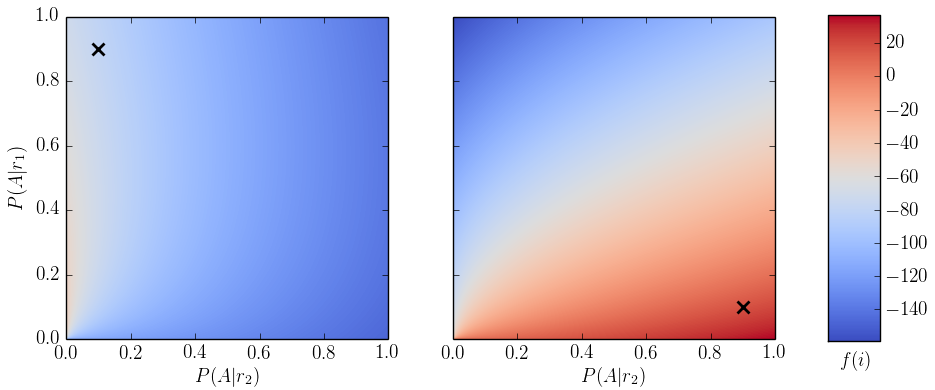
\includegraphics[width=\textwidth]{objective_function_cropped.png}
\scalebox{.65}{%% Creator: Matplotlib, PGF backend
%%
%% To include the figure in your LaTeX document, write
%%   \input{<filename>.pgf}
%%
%% Make sure the required packages are loaded in your preamble
%%   \usepackage{pgf}
%%
%% Figures using additional raster images can only be included by \input if
%% they are in the same directory as the main LaTeX file. For loading figures
%% from other directories you can use the `import` package
%%   \usepackage{import}
%% and then include the figures with
%%   \import{<path to file>}{<filename>.pgf}
%%
%% Matplotlib used the following preamble
%%   \usepackage{fontspec}
%%   \setsansfont{DejaVu Sans}
%%   \setmonofont{DejaVu Sans Mono}
%%
\begingroup%
\makeatletter%
\begin{pgfpicture}%
\pgfpathrectangle{\pgfpointorigin}{\pgfqpoint{8.150000in}{4.075000in}}%
\pgfusepath{use as bounding box, clip}%
\begin{pgfscope}%
\pgfsetbuttcap%
\pgfsetmiterjoin%
\definecolor{currentfill}{rgb}{1.000000,1.000000,1.000000}%
\pgfsetfillcolor{currentfill}%
\pgfsetlinewidth{0.000000pt}%
\definecolor{currentstroke}{rgb}{1.000000,1.000000,1.000000}%
\pgfsetstrokecolor{currentstroke}%
\pgfsetdash{}{0pt}%
\pgfpathmoveto{\pgfqpoint{0.000000in}{0.000000in}}%
\pgfpathlineto{\pgfqpoint{8.150000in}{0.000000in}}%
\pgfpathlineto{\pgfqpoint{8.150000in}{4.075000in}}%
\pgfpathlineto{\pgfqpoint{0.000000in}{4.075000in}}%
\pgfpathclose%
\pgfusepath{fill}%
\end{pgfscope}%
\begin{pgfscope}%
\pgfsetbuttcap%
\pgfsetmiterjoin%
\definecolor{currentfill}{rgb}{1.000000,1.000000,1.000000}%
\pgfsetfillcolor{currentfill}%
\pgfsetlinewidth{0.000000pt}%
\definecolor{currentstroke}{rgb}{0.000000,0.000000,0.000000}%
\pgfsetstrokecolor{currentstroke}%
\pgfsetstrokeopacity{0.000000}%
\pgfsetdash{}{0pt}%
\pgfpathmoveto{\pgfqpoint{1.018750in}{0.407500in}}%
\pgfpathlineto{\pgfqpoint{7.335000in}{0.407500in}}%
\pgfpathlineto{\pgfqpoint{7.335000in}{3.667500in}}%
\pgfpathlineto{\pgfqpoint{1.018750in}{3.667500in}}%
\pgfpathclose%
\pgfusepath{fill}%
\end{pgfscope}%
\begin{pgfscope}%
\pgfpathrectangle{\pgfqpoint{1.018750in}{0.407500in}}{\pgfqpoint{6.316250in}{3.260000in}} %
\pgfusepath{clip}%
\pgfsetbuttcap%
\pgfsetmiterjoin%
\definecolor{currentfill}{rgb}{0.200000,0.200000,0.200000}%
\pgfsetfillcolor{currentfill}%
\pgfsetlinewidth{1.003750pt}%
\definecolor{currentstroke}{rgb}{0.000000,0.000000,0.000000}%
\pgfsetstrokecolor{currentstroke}%
\pgfsetdash{}{0pt}%
\pgfpathmoveto{\pgfqpoint{1.176656in}{-2.200500in}}%
\pgfpathmoveto{\pgfqpoint{1.492469in}{0.397500in}}%
\pgfpathlineto{\pgfqpoint{1.492469in}{2.589200in}}%
\pgfpathlineto{\pgfqpoint{1.176656in}{2.589200in}}%
\pgfpathlineto{\pgfqpoint{1.176656in}{-2.200500in}}%
\pgfusepath{stroke,fill}%
\end{pgfscope}%
\begin{pgfscope}%
\pgfpathrectangle{\pgfqpoint{1.018750in}{0.407500in}}{\pgfqpoint{6.316250in}{3.260000in}} %
\pgfusepath{clip}%
\pgfsetbuttcap%
\pgfsetmiterjoin%
\definecolor{currentfill}{rgb}{0.200000,0.200000,0.200000}%
\pgfsetfillcolor{currentfill}%
\pgfsetlinewidth{1.003750pt}%
\definecolor{currentstroke}{rgb}{0.000000,0.000000,0.000000}%
\pgfsetstrokecolor{currentstroke}%
\pgfsetdash{}{0pt}%
\pgfpathmoveto{\pgfqpoint{2.755719in}{-2.200500in}}%
\pgfpathmoveto{\pgfqpoint{3.071531in}{0.397500in}}%
\pgfpathlineto{\pgfqpoint{3.071531in}{1.211733in}}%
\pgfpathlineto{\pgfqpoint{2.755719in}{1.211733in}}%
\pgfpathlineto{\pgfqpoint{2.755719in}{-2.200500in}}%
\pgfusepath{stroke,fill}%
\end{pgfscope}%
\begin{pgfscope}%
\pgfpathrectangle{\pgfqpoint{1.018750in}{0.407500in}}{\pgfqpoint{6.316250in}{3.260000in}} %
\pgfusepath{clip}%
\pgfsetbuttcap%
\pgfsetmiterjoin%
\definecolor{currentfill}{rgb}{0.200000,0.200000,0.200000}%
\pgfsetfillcolor{currentfill}%
\pgfsetlinewidth{1.003750pt}%
\definecolor{currentstroke}{rgb}{0.000000,0.000000,0.000000}%
\pgfsetstrokecolor{currentstroke}%
\pgfsetdash{}{0pt}%
\pgfpathmoveto{\pgfqpoint{4.334781in}{-2.200500in}}%
\pgfpathmoveto{\pgfqpoint{4.650594in}{0.397500in}}%
\pgfpathlineto{\pgfqpoint{4.650594in}{2.349143in}}%
\pgfpathlineto{\pgfqpoint{4.334781in}{2.349143in}}%
\pgfpathlineto{\pgfqpoint{4.334781in}{-2.200500in}}%
\pgfusepath{stroke,fill}%
\end{pgfscope}%
\begin{pgfscope}%
\pgfpathrectangle{\pgfqpoint{1.018750in}{0.407500in}}{\pgfqpoint{6.316250in}{3.260000in}} %
\pgfusepath{clip}%
\pgfsetbuttcap%
\pgfsetmiterjoin%
\definecolor{currentfill}{rgb}{0.200000,0.200000,0.200000}%
\pgfsetfillcolor{currentfill}%
\pgfsetlinewidth{1.003750pt}%
\definecolor{currentstroke}{rgb}{0.000000,0.000000,0.000000}%
\pgfsetstrokecolor{currentstroke}%
\pgfsetdash{}{0pt}%
\pgfpathmoveto{\pgfqpoint{5.913844in}{-2.200500in}}%
\pgfpathmoveto{\pgfqpoint{6.229656in}{0.397500in}}%
\pgfpathlineto{\pgfqpoint{6.229656in}{0.920235in}}%
\pgfpathlineto{\pgfqpoint{5.913844in}{0.920235in}}%
\pgfpathlineto{\pgfqpoint{5.913844in}{-2.200500in}}%
\pgfusepath{stroke,fill}%
\end{pgfscope}%
\begin{pgfscope}%
\pgfpathrectangle{\pgfqpoint{1.018750in}{0.407500in}}{\pgfqpoint{6.316250in}{3.260000in}} %
\pgfusepath{clip}%
\pgfsetbuttcap%
\pgfsetmiterjoin%
\definecolor{currentfill}{rgb}{0.400000,0.400000,0.400000}%
\pgfsetfillcolor{currentfill}%
\pgfsetlinewidth{1.003750pt}%
\definecolor{currentstroke}{rgb}{0.000000,0.000000,0.000000}%
\pgfsetstrokecolor{currentstroke}%
\pgfsetdash{}{0pt}%
\pgfpathmoveto{\pgfqpoint{1.492469in}{-2.200500in}}%
\pgfpathmoveto{\pgfqpoint{1.808281in}{0.397500in}}%
\pgfpathlineto{\pgfqpoint{1.808281in}{2.215002in}}%
\pgfpathlineto{\pgfqpoint{1.492469in}{2.215002in}}%
\pgfpathlineto{\pgfqpoint{1.492469in}{-2.200500in}}%
\pgfusepath{stroke,fill}%
\end{pgfscope}%
\begin{pgfscope}%
\pgfpathrectangle{\pgfqpoint{1.018750in}{0.407500in}}{\pgfqpoint{6.316250in}{3.260000in}} %
\pgfusepath{clip}%
\pgfsetbuttcap%
\pgfsetmiterjoin%
\definecolor{currentfill}{rgb}{0.400000,0.400000,0.400000}%
\pgfsetfillcolor{currentfill}%
\pgfsetlinewidth{1.003750pt}%
\definecolor{currentstroke}{rgb}{0.000000,0.000000,0.000000}%
\pgfsetstrokecolor{currentstroke}%
\pgfsetdash{}{0pt}%
\pgfpathmoveto{\pgfqpoint{3.071531in}{-2.200500in}}%
\pgfpathmoveto{\pgfqpoint{3.387344in}{0.397500in}}%
\pgfpathlineto{\pgfqpoint{3.387344in}{1.497483in}}%
\pgfpathlineto{\pgfqpoint{3.071531in}{1.497483in}}%
\pgfpathlineto{\pgfqpoint{3.071531in}{-2.200500in}}%
\pgfusepath{stroke,fill}%
\end{pgfscope}%
\begin{pgfscope}%
\pgfpathrectangle{\pgfqpoint{1.018750in}{0.407500in}}{\pgfqpoint{6.316250in}{3.260000in}} %
\pgfusepath{clip}%
\pgfsetbuttcap%
\pgfsetmiterjoin%
\definecolor{currentfill}{rgb}{0.400000,0.400000,0.400000}%
\pgfsetfillcolor{currentfill}%
\pgfsetlinewidth{1.003750pt}%
\definecolor{currentstroke}{rgb}{0.000000,0.000000,0.000000}%
\pgfsetstrokecolor{currentstroke}%
\pgfsetdash{}{0pt}%
\pgfpathmoveto{\pgfqpoint{4.650594in}{-2.200500in}}%
\pgfpathmoveto{\pgfqpoint{4.966406in}{0.397500in}}%
\pgfpathlineto{\pgfqpoint{4.966406in}{2.159808in}}%
\pgfpathlineto{\pgfqpoint{4.650594in}{2.159808in}}%
\pgfpathlineto{\pgfqpoint{4.650594in}{-2.200500in}}%
\pgfusepath{stroke,fill}%
\end{pgfscope}%
\begin{pgfscope}%
\pgfpathrectangle{\pgfqpoint{1.018750in}{0.407500in}}{\pgfqpoint{6.316250in}{3.260000in}} %
\pgfusepath{clip}%
\pgfsetbuttcap%
\pgfsetmiterjoin%
\definecolor{currentfill}{rgb}{0.400000,0.400000,0.400000}%
\pgfsetfillcolor{currentfill}%
\pgfsetlinewidth{1.003750pt}%
\definecolor{currentstroke}{rgb}{0.000000,0.000000,0.000000}%
\pgfsetstrokecolor{currentstroke}%
\pgfsetdash{}{0pt}%
\pgfpathmoveto{\pgfqpoint{6.229656in}{-2.200500in}}%
\pgfpathmoveto{\pgfqpoint{6.545469in}{0.397500in}}%
\pgfpathlineto{\pgfqpoint{6.545469in}{1.387095in}}%
\pgfpathlineto{\pgfqpoint{6.229656in}{1.387095in}}%
\pgfpathlineto{\pgfqpoint{6.229656in}{-2.200500in}}%
\pgfusepath{stroke,fill}%
\end{pgfscope}%
\begin{pgfscope}%
\pgfpathrectangle{\pgfqpoint{1.018750in}{0.407500in}}{\pgfqpoint{6.316250in}{3.260000in}} %
\pgfusepath{clip}%
\pgfsetbuttcap%
\pgfsetmiterjoin%
\definecolor{currentfill}{rgb}{0.600000,0.600000,0.600000}%
\pgfsetfillcolor{currentfill}%
\pgfsetlinewidth{1.003750pt}%
\definecolor{currentstroke}{rgb}{0.000000,0.000000,0.000000}%
\pgfsetstrokecolor{currentstroke}%
\pgfsetdash{}{0pt}%
\pgfpathmoveto{\pgfqpoint{1.808281in}{-2.200500in}}%
\pgfpathmoveto{\pgfqpoint{2.124094in}{0.397500in}}%
\pgfpathlineto{\pgfqpoint{2.124094in}{1.966887in}}%
\pgfpathlineto{\pgfqpoint{1.808281in}{1.966887in}}%
\pgfpathlineto{\pgfqpoint{1.808281in}{-2.200500in}}%
\pgfusepath{stroke,fill}%
\end{pgfscope}%
\begin{pgfscope}%
\pgfpathrectangle{\pgfqpoint{1.018750in}{0.407500in}}{\pgfqpoint{6.316250in}{3.260000in}} %
\pgfusepath{clip}%
\pgfsetbuttcap%
\pgfsetmiterjoin%
\definecolor{currentfill}{rgb}{0.600000,0.600000,0.600000}%
\pgfsetfillcolor{currentfill}%
\pgfsetlinewidth{1.003750pt}%
\definecolor{currentstroke}{rgb}{0.000000,0.000000,0.000000}%
\pgfsetstrokecolor{currentstroke}%
\pgfsetdash{}{0pt}%
\pgfpathmoveto{\pgfqpoint{3.387344in}{-2.200500in}}%
\pgfpathmoveto{\pgfqpoint{3.703156in}{0.397500in}}%
\pgfpathlineto{\pgfqpoint{3.703156in}{1.109765in}}%
\pgfpathlineto{\pgfqpoint{3.387344in}{1.109765in}}%
\pgfpathlineto{\pgfqpoint{3.387344in}{-2.200500in}}%
\pgfusepath{stroke,fill}%
\end{pgfscope}%
\begin{pgfscope}%
\pgfpathrectangle{\pgfqpoint{1.018750in}{0.407500in}}{\pgfqpoint{6.316250in}{3.260000in}} %
\pgfusepath{clip}%
\pgfsetbuttcap%
\pgfsetmiterjoin%
\definecolor{currentfill}{rgb}{0.600000,0.600000,0.600000}%
\pgfsetfillcolor{currentfill}%
\pgfsetlinewidth{1.003750pt}%
\definecolor{currentstroke}{rgb}{0.000000,0.000000,0.000000}%
\pgfsetstrokecolor{currentstroke}%
\pgfsetdash{}{0pt}%
\pgfpathmoveto{\pgfqpoint{4.966406in}{-2.200500in}}%
\pgfpathmoveto{\pgfqpoint{5.282219in}{0.397500in}}%
\pgfpathlineto{\pgfqpoint{5.282219in}{2.410226in}}%
\pgfpathlineto{\pgfqpoint{4.966406in}{2.410226in}}%
\pgfpathlineto{\pgfqpoint{4.966406in}{-2.200500in}}%
\pgfusepath{stroke,fill}%
\end{pgfscope}%
\begin{pgfscope}%
\pgfpathrectangle{\pgfqpoint{1.018750in}{0.407500in}}{\pgfqpoint{6.316250in}{3.260000in}} %
\pgfusepath{clip}%
\pgfsetbuttcap%
\pgfsetmiterjoin%
\definecolor{currentfill}{rgb}{0.600000,0.600000,0.600000}%
\pgfsetfillcolor{currentfill}%
\pgfsetlinewidth{1.003750pt}%
\definecolor{currentstroke}{rgb}{0.000000,0.000000,0.000000}%
\pgfsetstrokecolor{currentstroke}%
\pgfsetdash{}{0pt}%
\pgfpathmoveto{\pgfqpoint{6.545469in}{-2.200500in}}%
\pgfpathmoveto{\pgfqpoint{6.861281in}{0.397500in}}%
\pgfpathlineto{\pgfqpoint{6.861281in}{1.671328in}}%
\pgfpathlineto{\pgfqpoint{6.545469in}{1.671328in}}%
\pgfpathlineto{\pgfqpoint{6.545469in}{-2.200500in}}%
\pgfusepath{stroke,fill}%
\end{pgfscope}%
\begin{pgfscope}%
\pgfpathrectangle{\pgfqpoint{1.018750in}{0.407500in}}{\pgfqpoint{6.316250in}{3.260000in}} %
\pgfusepath{clip}%
\pgfsetbuttcap%
\pgfsetmiterjoin%
\definecolor{currentfill}{rgb}{0.800000,0.800000,0.800000}%
\pgfsetfillcolor{currentfill}%
\pgfsetlinewidth{1.003750pt}%
\definecolor{currentstroke}{rgb}{0.000000,0.000000,0.000000}%
\pgfsetstrokecolor{currentstroke}%
\pgfsetdash{}{0pt}%
\pgfpathmoveto{\pgfqpoint{2.124094in}{-2.200500in}}%
\pgfpathmoveto{\pgfqpoint{2.439906in}{0.397500in}}%
\pgfpathlineto{\pgfqpoint{2.439906in}{1.711500in}}%
\pgfpathlineto{\pgfqpoint{2.124094in}{1.711500in}}%
\pgfpathlineto{\pgfqpoint{2.124094in}{-2.200500in}}%
\pgfusepath{stroke,fill}%
\end{pgfscope}%
\begin{pgfscope}%
\pgfpathrectangle{\pgfqpoint{1.018750in}{0.407500in}}{\pgfqpoint{6.316250in}{3.260000in}} %
\pgfusepath{clip}%
\pgfsetbuttcap%
\pgfsetmiterjoin%
\definecolor{currentfill}{rgb}{0.800000,0.800000,0.800000}%
\pgfsetfillcolor{currentfill}%
\pgfsetlinewidth{1.003750pt}%
\definecolor{currentstroke}{rgb}{0.000000,0.000000,0.000000}%
\pgfsetstrokecolor{currentstroke}%
\pgfsetdash{}{0pt}%
\pgfpathmoveto{\pgfqpoint{3.703156in}{-2.200500in}}%
\pgfpathmoveto{\pgfqpoint{4.018969in}{0.397500in}}%
\pgfpathlineto{\pgfqpoint{4.018969in}{1.059500in}}%
\pgfpathlineto{\pgfqpoint{3.703156in}{1.059500in}}%
\pgfpathlineto{\pgfqpoint{3.703156in}{-2.200500in}}%
\pgfusepath{stroke,fill}%
\end{pgfscope}%
\begin{pgfscope}%
\pgfpathrectangle{\pgfqpoint{1.018750in}{0.407500in}}{\pgfqpoint{6.316250in}{3.260000in}} %
\pgfusepath{clip}%
\pgfsetbuttcap%
\pgfsetmiterjoin%
\definecolor{currentfill}{rgb}{0.800000,0.800000,0.800000}%
\pgfsetfillcolor{currentfill}%
\pgfsetlinewidth{1.003750pt}%
\definecolor{currentstroke}{rgb}{0.000000,0.000000,0.000000}%
\pgfsetstrokecolor{currentstroke}%
\pgfsetdash{}{0pt}%
\pgfpathmoveto{\pgfqpoint{5.282219in}{-2.200500in}}%
\pgfpathmoveto{\pgfqpoint{5.598031in}{0.397500in}}%
\pgfpathlineto{\pgfqpoint{5.598031in}{3.015500in}}%
\pgfpathlineto{\pgfqpoint{5.282219in}{3.015500in}}%
\pgfpathlineto{\pgfqpoint{5.282219in}{-2.200500in}}%
\pgfusepath{stroke,fill}%
\end{pgfscope}%
\begin{pgfscope}%
\pgfpathrectangle{\pgfqpoint{1.018750in}{0.407500in}}{\pgfqpoint{6.316250in}{3.260000in}} %
\pgfusepath{clip}%
\pgfsetbuttcap%
\pgfsetmiterjoin%
\definecolor{currentfill}{rgb}{0.800000,0.800000,0.800000}%
\pgfsetfillcolor{currentfill}%
\pgfsetlinewidth{1.003750pt}%
\definecolor{currentstroke}{rgb}{0.000000,0.000000,0.000000}%
\pgfsetstrokecolor{currentstroke}%
\pgfsetdash{}{0pt}%
\pgfpathmoveto{\pgfqpoint{6.861281in}{-2.200500in}}%
\pgfpathmoveto{\pgfqpoint{7.177094in}{0.397500in}}%
\pgfpathlineto{\pgfqpoint{7.177094in}{1.059500in}}%
\pgfpathlineto{\pgfqpoint{6.861281in}{1.059500in}}%
\pgfpathlineto{\pgfqpoint{6.861281in}{-2.200500in}}%
\pgfusepath{stroke,fill}%
\end{pgfscope}%
\begin{pgfscope}%
\pgfsetrectcap%
\pgfsetmiterjoin%
\pgfsetlinewidth{1.003750pt}%
\definecolor{currentstroke}{rgb}{0.000000,0.000000,0.000000}%
\pgfsetstrokecolor{currentstroke}%
\pgfsetdash{}{0pt}%
\pgfpathmoveto{\pgfqpoint{1.018750in}{3.667500in}}%
\pgfpathlineto{\pgfqpoint{7.335000in}{3.667500in}}%
\pgfusepath{stroke}%
\end{pgfscope}%
\begin{pgfscope}%
\pgfsetrectcap%
\pgfsetmiterjoin%
\pgfsetlinewidth{1.003750pt}%
\definecolor{currentstroke}{rgb}{0.000000,0.000000,0.000000}%
\pgfsetstrokecolor{currentstroke}%
\pgfsetdash{}{0pt}%
\pgfpathmoveto{\pgfqpoint{7.335000in}{0.407500in}}%
\pgfpathlineto{\pgfqpoint{7.335000in}{3.667500in}}%
\pgfusepath{stroke}%
\end{pgfscope}%
\begin{pgfscope}%
\pgfsetrectcap%
\pgfsetmiterjoin%
\pgfsetlinewidth{1.003750pt}%
\definecolor{currentstroke}{rgb}{0.000000,0.000000,0.000000}%
\pgfsetstrokecolor{currentstroke}%
\pgfsetdash{}{0pt}%
\pgfpathmoveto{\pgfqpoint{1.018750in}{0.407500in}}%
\pgfpathlineto{\pgfqpoint{7.335000in}{0.407500in}}%
\pgfusepath{stroke}%
\end{pgfscope}%
\begin{pgfscope}%
\pgfsetrectcap%
\pgfsetmiterjoin%
\pgfsetlinewidth{1.003750pt}%
\definecolor{currentstroke}{rgb}{0.000000,0.000000,0.000000}%
\pgfsetstrokecolor{currentstroke}%
\pgfsetdash{}{0pt}%
\pgfpathmoveto{\pgfqpoint{1.018750in}{0.407500in}}%
\pgfpathlineto{\pgfqpoint{1.018750in}{3.667500in}}%
\pgfusepath{stroke}%
\end{pgfscope}%
\begin{pgfscope}%
\pgfsetbuttcap%
\pgfsetroundjoin%
\definecolor{currentfill}{rgb}{0.000000,0.000000,0.000000}%
\pgfsetfillcolor{currentfill}%
\pgfsetlinewidth{0.501875pt}%
\definecolor{currentstroke}{rgb}{0.000000,0.000000,0.000000}%
\pgfsetstrokecolor{currentstroke}%
\pgfsetdash{}{0pt}%
\pgfsys@defobject{currentmarker}{\pgfqpoint{0.000000in}{0.000000in}}{\pgfqpoint{0.000000in}{0.055556in}}{%
\pgfpathmoveto{\pgfqpoint{0.000000in}{0.000000in}}%
\pgfpathlineto{\pgfqpoint{0.000000in}{0.055556in}}%
\pgfusepath{stroke,fill}%
}%
\begin{pgfscope}%
\pgfsys@transformshift{1.808281in}{0.407500in}%
\pgfsys@useobject{currentmarker}{}%
\end{pgfscope}%
\end{pgfscope}%
\begin{pgfscope}%
\pgfsetbuttcap%
\pgfsetroundjoin%
\definecolor{currentfill}{rgb}{0.000000,0.000000,0.000000}%
\pgfsetfillcolor{currentfill}%
\pgfsetlinewidth{0.501875pt}%
\definecolor{currentstroke}{rgb}{0.000000,0.000000,0.000000}%
\pgfsetstrokecolor{currentstroke}%
\pgfsetdash{}{0pt}%
\pgfsys@defobject{currentmarker}{\pgfqpoint{0.000000in}{-0.055556in}}{\pgfqpoint{0.000000in}{0.000000in}}{%
\pgfpathmoveto{\pgfqpoint{0.000000in}{0.000000in}}%
\pgfpathlineto{\pgfqpoint{0.000000in}{-0.055556in}}%
\pgfusepath{stroke,fill}%
}%
\begin{pgfscope}%
\pgfsys@transformshift{1.808281in}{3.667500in}%
\pgfsys@useobject{currentmarker}{}%
\end{pgfscope}%
\end{pgfscope}%
\begin{pgfscope}%
\pgftext[x=1.808281in,y=0.351944in,,top]{{\sffamily\fontsize{14.000000}{16.800000}\selectfont \textrm{Experiment 1}}}%
\end{pgfscope}%
\begin{pgfscope}%
\pgfsetbuttcap%
\pgfsetroundjoin%
\definecolor{currentfill}{rgb}{0.000000,0.000000,0.000000}%
\pgfsetfillcolor{currentfill}%
\pgfsetlinewidth{0.501875pt}%
\definecolor{currentstroke}{rgb}{0.000000,0.000000,0.000000}%
\pgfsetstrokecolor{currentstroke}%
\pgfsetdash{}{0pt}%
\pgfsys@defobject{currentmarker}{\pgfqpoint{0.000000in}{0.000000in}}{\pgfqpoint{0.000000in}{0.055556in}}{%
\pgfpathmoveto{\pgfqpoint{0.000000in}{0.000000in}}%
\pgfpathlineto{\pgfqpoint{0.000000in}{0.055556in}}%
\pgfusepath{stroke,fill}%
}%
\begin{pgfscope}%
\pgfsys@transformshift{3.387344in}{0.407500in}%
\pgfsys@useobject{currentmarker}{}%
\end{pgfscope}%
\end{pgfscope}%
\begin{pgfscope}%
\pgfsetbuttcap%
\pgfsetroundjoin%
\definecolor{currentfill}{rgb}{0.000000,0.000000,0.000000}%
\pgfsetfillcolor{currentfill}%
\pgfsetlinewidth{0.501875pt}%
\definecolor{currentstroke}{rgb}{0.000000,0.000000,0.000000}%
\pgfsetstrokecolor{currentstroke}%
\pgfsetdash{}{0pt}%
\pgfsys@defobject{currentmarker}{\pgfqpoint{0.000000in}{-0.055556in}}{\pgfqpoint{0.000000in}{0.000000in}}{%
\pgfpathmoveto{\pgfqpoint{0.000000in}{0.000000in}}%
\pgfpathlineto{\pgfqpoint{0.000000in}{-0.055556in}}%
\pgfusepath{stroke,fill}%
}%
\begin{pgfscope}%
\pgfsys@transformshift{3.387344in}{3.667500in}%
\pgfsys@useobject{currentmarker}{}%
\end{pgfscope}%
\end{pgfscope}%
\begin{pgfscope}%
\pgftext[x=3.387344in,y=0.351944in,,top]{{\sffamily\fontsize{14.000000}{16.800000}\selectfont \textrm{Experiment 2}}}%
\end{pgfscope}%
\begin{pgfscope}%
\pgfsetbuttcap%
\pgfsetroundjoin%
\definecolor{currentfill}{rgb}{0.000000,0.000000,0.000000}%
\pgfsetfillcolor{currentfill}%
\pgfsetlinewidth{0.501875pt}%
\definecolor{currentstroke}{rgb}{0.000000,0.000000,0.000000}%
\pgfsetstrokecolor{currentstroke}%
\pgfsetdash{}{0pt}%
\pgfsys@defobject{currentmarker}{\pgfqpoint{0.000000in}{0.000000in}}{\pgfqpoint{0.000000in}{0.055556in}}{%
\pgfpathmoveto{\pgfqpoint{0.000000in}{0.000000in}}%
\pgfpathlineto{\pgfqpoint{0.000000in}{0.055556in}}%
\pgfusepath{stroke,fill}%
}%
\begin{pgfscope}%
\pgfsys@transformshift{4.966406in}{0.407500in}%
\pgfsys@useobject{currentmarker}{}%
\end{pgfscope}%
\end{pgfscope}%
\begin{pgfscope}%
\pgfsetbuttcap%
\pgfsetroundjoin%
\definecolor{currentfill}{rgb}{0.000000,0.000000,0.000000}%
\pgfsetfillcolor{currentfill}%
\pgfsetlinewidth{0.501875pt}%
\definecolor{currentstroke}{rgb}{0.000000,0.000000,0.000000}%
\pgfsetstrokecolor{currentstroke}%
\pgfsetdash{}{0pt}%
\pgfsys@defobject{currentmarker}{\pgfqpoint{0.000000in}{-0.055556in}}{\pgfqpoint{0.000000in}{0.000000in}}{%
\pgfpathmoveto{\pgfqpoint{0.000000in}{0.000000in}}%
\pgfpathlineto{\pgfqpoint{0.000000in}{-0.055556in}}%
\pgfusepath{stroke,fill}%
}%
\begin{pgfscope}%
\pgfsys@transformshift{4.966406in}{3.667500in}%
\pgfsys@useobject{currentmarker}{}%
\end{pgfscope}%
\end{pgfscope}%
\begin{pgfscope}%
\pgftext[x=4.966406in,y=0.351944in,,top]{{\sffamily\fontsize{14.000000}{16.800000}\selectfont \textrm{Experiment 3}}}%
\end{pgfscope}%
\begin{pgfscope}%
\pgfsetbuttcap%
\pgfsetroundjoin%
\definecolor{currentfill}{rgb}{0.000000,0.000000,0.000000}%
\pgfsetfillcolor{currentfill}%
\pgfsetlinewidth{0.501875pt}%
\definecolor{currentstroke}{rgb}{0.000000,0.000000,0.000000}%
\pgfsetstrokecolor{currentstroke}%
\pgfsetdash{}{0pt}%
\pgfsys@defobject{currentmarker}{\pgfqpoint{0.000000in}{0.000000in}}{\pgfqpoint{0.000000in}{0.055556in}}{%
\pgfpathmoveto{\pgfqpoint{0.000000in}{0.000000in}}%
\pgfpathlineto{\pgfqpoint{0.000000in}{0.055556in}}%
\pgfusepath{stroke,fill}%
}%
\begin{pgfscope}%
\pgfsys@transformshift{6.545469in}{0.407500in}%
\pgfsys@useobject{currentmarker}{}%
\end{pgfscope}%
\end{pgfscope}%
\begin{pgfscope}%
\pgfsetbuttcap%
\pgfsetroundjoin%
\definecolor{currentfill}{rgb}{0.000000,0.000000,0.000000}%
\pgfsetfillcolor{currentfill}%
\pgfsetlinewidth{0.501875pt}%
\definecolor{currentstroke}{rgb}{0.000000,0.000000,0.000000}%
\pgfsetstrokecolor{currentstroke}%
\pgfsetdash{}{0pt}%
\pgfsys@defobject{currentmarker}{\pgfqpoint{0.000000in}{-0.055556in}}{\pgfqpoint{0.000000in}{0.000000in}}{%
\pgfpathmoveto{\pgfqpoint{0.000000in}{0.000000in}}%
\pgfpathlineto{\pgfqpoint{0.000000in}{-0.055556in}}%
\pgfusepath{stroke,fill}%
}%
\begin{pgfscope}%
\pgfsys@transformshift{6.545469in}{3.667500in}%
\pgfsys@useobject{currentmarker}{}%
\end{pgfscope}%
\end{pgfscope}%
\begin{pgfscope}%
\pgftext[x=6.545469in,y=0.351944in,,top]{{\sffamily\fontsize{14.000000}{16.800000}\selectfont \textrm{Experiment 4}}}%
\end{pgfscope}%
\begin{pgfscope}%
\pgfsetbuttcap%
\pgfsetroundjoin%
\definecolor{currentfill}{rgb}{0.000000,0.000000,0.000000}%
\pgfsetfillcolor{currentfill}%
\pgfsetlinewidth{0.501875pt}%
\definecolor{currentstroke}{rgb}{0.000000,0.000000,0.000000}%
\pgfsetstrokecolor{currentstroke}%
\pgfsetdash{}{0pt}%
\pgfsys@defobject{currentmarker}{\pgfqpoint{0.000000in}{0.000000in}}{\pgfqpoint{0.055556in}{0.000000in}}{%
\pgfpathmoveto{\pgfqpoint{0.000000in}{0.000000in}}%
\pgfpathlineto{\pgfqpoint{0.055556in}{0.000000in}}%
\pgfusepath{stroke,fill}%
}%
\begin{pgfscope}%
\pgfsys@transformshift{1.018750in}{0.407500in}%
\pgfsys@useobject{currentmarker}{}%
\end{pgfscope}%
\end{pgfscope}%
\begin{pgfscope}%
\pgfsetbuttcap%
\pgfsetroundjoin%
\definecolor{currentfill}{rgb}{0.000000,0.000000,0.000000}%
\pgfsetfillcolor{currentfill}%
\pgfsetlinewidth{0.501875pt}%
\definecolor{currentstroke}{rgb}{0.000000,0.000000,0.000000}%
\pgfsetstrokecolor{currentstroke}%
\pgfsetdash{}{0pt}%
\pgfsys@defobject{currentmarker}{\pgfqpoint{-0.055556in}{0.000000in}}{\pgfqpoint{0.000000in}{0.000000in}}{%
\pgfpathmoveto{\pgfqpoint{0.000000in}{0.000000in}}%
\pgfpathlineto{\pgfqpoint{-0.055556in}{0.000000in}}%
\pgfusepath{stroke,fill}%
}%
\begin{pgfscope}%
\pgfsys@transformshift{7.335000in}{0.407500in}%
\pgfsys@useobject{currentmarker}{}%
\end{pgfscope}%
\end{pgfscope}%
\begin{pgfscope}%
\pgftext[x=0.963194in,y=0.407500in,right,]{{\sffamily\fontsize{14.000000}{16.800000}\selectfont \(\displaystyle 40\%\)}}%
\end{pgfscope}%
\begin{pgfscope}%
\pgfsetbuttcap%
\pgfsetroundjoin%
\definecolor{currentfill}{rgb}{0.000000,0.000000,0.000000}%
\pgfsetfillcolor{currentfill}%
\pgfsetlinewidth{0.501875pt}%
\definecolor{currentstroke}{rgb}{0.000000,0.000000,0.000000}%
\pgfsetstrokecolor{currentstroke}%
\pgfsetdash{}{0pt}%
\pgfsys@defobject{currentmarker}{\pgfqpoint{0.000000in}{0.000000in}}{\pgfqpoint{0.055556in}{0.000000in}}{%
\pgfpathmoveto{\pgfqpoint{0.000000in}{0.000000in}}%
\pgfpathlineto{\pgfqpoint{0.055556in}{0.000000in}}%
\pgfusepath{stroke,fill}%
}%
\begin{pgfscope}%
\pgfsys@transformshift{1.018750in}{1.059500in}%
\pgfsys@useobject{currentmarker}{}%
\end{pgfscope}%
\end{pgfscope}%
\begin{pgfscope}%
\pgfsetbuttcap%
\pgfsetroundjoin%
\definecolor{currentfill}{rgb}{0.000000,0.000000,0.000000}%
\pgfsetfillcolor{currentfill}%
\pgfsetlinewidth{0.501875pt}%
\definecolor{currentstroke}{rgb}{0.000000,0.000000,0.000000}%
\pgfsetstrokecolor{currentstroke}%
\pgfsetdash{}{0pt}%
\pgfsys@defobject{currentmarker}{\pgfqpoint{-0.055556in}{0.000000in}}{\pgfqpoint{0.000000in}{0.000000in}}{%
\pgfpathmoveto{\pgfqpoint{0.000000in}{0.000000in}}%
\pgfpathlineto{\pgfqpoint{-0.055556in}{0.000000in}}%
\pgfusepath{stroke,fill}%
}%
\begin{pgfscope}%
\pgfsys@transformshift{7.335000in}{1.059500in}%
\pgfsys@useobject{currentmarker}{}%
\end{pgfscope}%
\end{pgfscope}%
\begin{pgfscope}%
\pgftext[x=0.963194in,y=1.059500in,right,]{{\sffamily\fontsize{14.000000}{16.800000}\selectfont \(\displaystyle 50\%\)}}%
\end{pgfscope}%
\begin{pgfscope}%
\pgfsetbuttcap%
\pgfsetroundjoin%
\definecolor{currentfill}{rgb}{0.000000,0.000000,0.000000}%
\pgfsetfillcolor{currentfill}%
\pgfsetlinewidth{0.501875pt}%
\definecolor{currentstroke}{rgb}{0.000000,0.000000,0.000000}%
\pgfsetstrokecolor{currentstroke}%
\pgfsetdash{}{0pt}%
\pgfsys@defobject{currentmarker}{\pgfqpoint{0.000000in}{0.000000in}}{\pgfqpoint{0.055556in}{0.000000in}}{%
\pgfpathmoveto{\pgfqpoint{0.000000in}{0.000000in}}%
\pgfpathlineto{\pgfqpoint{0.055556in}{0.000000in}}%
\pgfusepath{stroke,fill}%
}%
\begin{pgfscope}%
\pgfsys@transformshift{1.018750in}{1.711500in}%
\pgfsys@useobject{currentmarker}{}%
\end{pgfscope}%
\end{pgfscope}%
\begin{pgfscope}%
\pgfsetbuttcap%
\pgfsetroundjoin%
\definecolor{currentfill}{rgb}{0.000000,0.000000,0.000000}%
\pgfsetfillcolor{currentfill}%
\pgfsetlinewidth{0.501875pt}%
\definecolor{currentstroke}{rgb}{0.000000,0.000000,0.000000}%
\pgfsetstrokecolor{currentstroke}%
\pgfsetdash{}{0pt}%
\pgfsys@defobject{currentmarker}{\pgfqpoint{-0.055556in}{0.000000in}}{\pgfqpoint{0.000000in}{0.000000in}}{%
\pgfpathmoveto{\pgfqpoint{0.000000in}{0.000000in}}%
\pgfpathlineto{\pgfqpoint{-0.055556in}{0.000000in}}%
\pgfusepath{stroke,fill}%
}%
\begin{pgfscope}%
\pgfsys@transformshift{7.335000in}{1.711500in}%
\pgfsys@useobject{currentmarker}{}%
\end{pgfscope}%
\end{pgfscope}%
\begin{pgfscope}%
\pgftext[x=0.963194in,y=1.711500in,right,]{{\sffamily\fontsize{14.000000}{16.800000}\selectfont \(\displaystyle 60\%\)}}%
\end{pgfscope}%
\begin{pgfscope}%
\pgfsetbuttcap%
\pgfsetroundjoin%
\definecolor{currentfill}{rgb}{0.000000,0.000000,0.000000}%
\pgfsetfillcolor{currentfill}%
\pgfsetlinewidth{0.501875pt}%
\definecolor{currentstroke}{rgb}{0.000000,0.000000,0.000000}%
\pgfsetstrokecolor{currentstroke}%
\pgfsetdash{}{0pt}%
\pgfsys@defobject{currentmarker}{\pgfqpoint{0.000000in}{0.000000in}}{\pgfqpoint{0.055556in}{0.000000in}}{%
\pgfpathmoveto{\pgfqpoint{0.000000in}{0.000000in}}%
\pgfpathlineto{\pgfqpoint{0.055556in}{0.000000in}}%
\pgfusepath{stroke,fill}%
}%
\begin{pgfscope}%
\pgfsys@transformshift{1.018750in}{2.363500in}%
\pgfsys@useobject{currentmarker}{}%
\end{pgfscope}%
\end{pgfscope}%
\begin{pgfscope}%
\pgfsetbuttcap%
\pgfsetroundjoin%
\definecolor{currentfill}{rgb}{0.000000,0.000000,0.000000}%
\pgfsetfillcolor{currentfill}%
\pgfsetlinewidth{0.501875pt}%
\definecolor{currentstroke}{rgb}{0.000000,0.000000,0.000000}%
\pgfsetstrokecolor{currentstroke}%
\pgfsetdash{}{0pt}%
\pgfsys@defobject{currentmarker}{\pgfqpoint{-0.055556in}{0.000000in}}{\pgfqpoint{0.000000in}{0.000000in}}{%
\pgfpathmoveto{\pgfqpoint{0.000000in}{0.000000in}}%
\pgfpathlineto{\pgfqpoint{-0.055556in}{0.000000in}}%
\pgfusepath{stroke,fill}%
}%
\begin{pgfscope}%
\pgfsys@transformshift{7.335000in}{2.363500in}%
\pgfsys@useobject{currentmarker}{}%
\end{pgfscope}%
\end{pgfscope}%
\begin{pgfscope}%
\pgftext[x=0.963194in,y=2.363500in,right,]{{\sffamily\fontsize{14.000000}{16.800000}\selectfont \(\displaystyle 70\%\)}}%
\end{pgfscope}%
\begin{pgfscope}%
\pgfsetbuttcap%
\pgfsetroundjoin%
\definecolor{currentfill}{rgb}{0.000000,0.000000,0.000000}%
\pgfsetfillcolor{currentfill}%
\pgfsetlinewidth{0.501875pt}%
\definecolor{currentstroke}{rgb}{0.000000,0.000000,0.000000}%
\pgfsetstrokecolor{currentstroke}%
\pgfsetdash{}{0pt}%
\pgfsys@defobject{currentmarker}{\pgfqpoint{0.000000in}{0.000000in}}{\pgfqpoint{0.055556in}{0.000000in}}{%
\pgfpathmoveto{\pgfqpoint{0.000000in}{0.000000in}}%
\pgfpathlineto{\pgfqpoint{0.055556in}{0.000000in}}%
\pgfusepath{stroke,fill}%
}%
\begin{pgfscope}%
\pgfsys@transformshift{1.018750in}{3.015500in}%
\pgfsys@useobject{currentmarker}{}%
\end{pgfscope}%
\end{pgfscope}%
\begin{pgfscope}%
\pgfsetbuttcap%
\pgfsetroundjoin%
\definecolor{currentfill}{rgb}{0.000000,0.000000,0.000000}%
\pgfsetfillcolor{currentfill}%
\pgfsetlinewidth{0.501875pt}%
\definecolor{currentstroke}{rgb}{0.000000,0.000000,0.000000}%
\pgfsetstrokecolor{currentstroke}%
\pgfsetdash{}{0pt}%
\pgfsys@defobject{currentmarker}{\pgfqpoint{-0.055556in}{0.000000in}}{\pgfqpoint{0.000000in}{0.000000in}}{%
\pgfpathmoveto{\pgfqpoint{0.000000in}{0.000000in}}%
\pgfpathlineto{\pgfqpoint{-0.055556in}{0.000000in}}%
\pgfusepath{stroke,fill}%
}%
\begin{pgfscope}%
\pgfsys@transformshift{7.335000in}{3.015500in}%
\pgfsys@useobject{currentmarker}{}%
\end{pgfscope}%
\end{pgfscope}%
\begin{pgfscope}%
\pgftext[x=0.963194in,y=3.015500in,right,]{{\sffamily\fontsize{14.000000}{16.800000}\selectfont \(\displaystyle 80\%\)}}%
\end{pgfscope}%
\begin{pgfscope}%
\pgfsetbuttcap%
\pgfsetroundjoin%
\definecolor{currentfill}{rgb}{0.000000,0.000000,0.000000}%
\pgfsetfillcolor{currentfill}%
\pgfsetlinewidth{0.501875pt}%
\definecolor{currentstroke}{rgb}{0.000000,0.000000,0.000000}%
\pgfsetstrokecolor{currentstroke}%
\pgfsetdash{}{0pt}%
\pgfsys@defobject{currentmarker}{\pgfqpoint{0.000000in}{0.000000in}}{\pgfqpoint{0.055556in}{0.000000in}}{%
\pgfpathmoveto{\pgfqpoint{0.000000in}{0.000000in}}%
\pgfpathlineto{\pgfqpoint{0.055556in}{0.000000in}}%
\pgfusepath{stroke,fill}%
}%
\begin{pgfscope}%
\pgfsys@transformshift{1.018750in}{3.667500in}%
\pgfsys@useobject{currentmarker}{}%
\end{pgfscope}%
\end{pgfscope}%
\begin{pgfscope}%
\pgfsetbuttcap%
\pgfsetroundjoin%
\definecolor{currentfill}{rgb}{0.000000,0.000000,0.000000}%
\pgfsetfillcolor{currentfill}%
\pgfsetlinewidth{0.501875pt}%
\definecolor{currentstroke}{rgb}{0.000000,0.000000,0.000000}%
\pgfsetstrokecolor{currentstroke}%
\pgfsetdash{}{0pt}%
\pgfsys@defobject{currentmarker}{\pgfqpoint{-0.055556in}{0.000000in}}{\pgfqpoint{0.000000in}{0.000000in}}{%
\pgfpathmoveto{\pgfqpoint{0.000000in}{0.000000in}}%
\pgfpathlineto{\pgfqpoint{-0.055556in}{0.000000in}}%
\pgfusepath{stroke,fill}%
}%
\begin{pgfscope}%
\pgfsys@transformshift{7.335000in}{3.667500in}%
\pgfsys@useobject{currentmarker}{}%
\end{pgfscope}%
\end{pgfscope}%
\begin{pgfscope}%
\pgftext[x=0.963194in,y=3.667500in,right,]{{\sffamily\fontsize{14.000000}{16.800000}\selectfont \(\displaystyle 90\%\)}}%
\end{pgfscope}%
\begin{pgfscope}%
\pgftext[x=0.539253in,y=2.037500in,,bottom,rotate=90.000000]{{\sffamily\fontsize{14.000000}{16.800000}\selectfont \textrm{Ambiguous form coordination rate (scaled)}}}%
\end{pgfscope}%
\begin{pgfscope}%
\pgfsetbuttcap%
\pgfsetmiterjoin%
\definecolor{currentfill}{rgb}{1.000000,1.000000,1.000000}%
\pgfsetfillcolor{currentfill}%
\pgfsetlinewidth{1.003750pt}%
\definecolor{currentstroke}{rgb}{0.000000,0.000000,0.000000}%
\pgfsetstrokecolor{currentstroke}%
\pgfsetdash{}{0pt}%
\pgfpathmoveto{\pgfqpoint{1.911014in}{3.130889in}}%
\pgfpathlineto{\pgfqpoint{6.442736in}{3.130889in}}%
\pgfpathlineto{\pgfqpoint{6.442736in}{3.733278in}}%
\pgfpathlineto{\pgfqpoint{1.911014in}{3.733278in}}%
\pgfpathclose%
\pgfusepath{stroke,fill}%
\end{pgfscope}%
\begin{pgfscope}%
\pgfsetbuttcap%
\pgfsetmiterjoin%
\definecolor{currentfill}{rgb}{0.200000,0.200000,0.200000}%
\pgfsetfillcolor{currentfill}%
\pgfsetlinewidth{1.003750pt}%
\definecolor{currentstroke}{rgb}{0.000000,0.000000,0.000000}%
\pgfsetstrokecolor{currentstroke}%
\pgfsetdash{}{0pt}%
\pgfpathmoveto{\pgfqpoint{1.988792in}{3.519389in}}%
\pgfpathlineto{\pgfqpoint{2.377681in}{3.519389in}}%
\pgfpathlineto{\pgfqpoint{2.377681in}{3.655500in}}%
\pgfpathlineto{\pgfqpoint{1.988792in}{3.655500in}}%
\pgfpathclose%
\pgfusepath{stroke,fill}%
\end{pgfscope}%
\begin{pgfscope}%
\pgftext[x=2.533236in,y=3.519389in,left,base]{{\rmfamily\fontsize{14.000000}{16.800000}\selectfont Repair model}}%
\end{pgfscope}%
\begin{pgfscope}%
\pgfsetbuttcap%
\pgfsetmiterjoin%
\definecolor{currentfill}{rgb}{0.400000,0.400000,0.400000}%
\pgfsetfillcolor{currentfill}%
\pgfsetlinewidth{1.003750pt}%
\definecolor{currentstroke}{rgb}{0.000000,0.000000,0.000000}%
\pgfsetstrokecolor{currentstroke}%
\pgfsetdash{}{0pt}%
\pgfpathmoveto{\pgfqpoint{1.988792in}{3.248333in}}%
\pgfpathlineto{\pgfqpoint{2.377681in}{3.248333in}}%
\pgfpathlineto{\pgfqpoint{2.377681in}{3.384445in}}%
\pgfpathlineto{\pgfqpoint{1.988792in}{3.384445in}}%
\pgfpathclose%
\pgfusepath{stroke,fill}%
\end{pgfscope}%
\begin{pgfscope}%
\pgftext[x=2.533236in,y=3.248333in,left,base]{{\rmfamily\fontsize{14.000000}{16.800000}\selectfont Rejection model}}%
\end{pgfscope}%
\begin{pgfscope}%
\pgfsetbuttcap%
\pgfsetmiterjoin%
\definecolor{currentfill}{rgb}{0.600000,0.600000,0.600000}%
\pgfsetfillcolor{currentfill}%
\pgfsetlinewidth{1.003750pt}%
\definecolor{currentstroke}{rgb}{0.000000,0.000000,0.000000}%
\pgfsetstrokecolor{currentstroke}%
\pgfsetdash{}{0pt}%
\pgfpathmoveto{\pgfqpoint{4.268069in}{3.519389in}}%
\pgfpathlineto{\pgfqpoint{4.656958in}{3.519389in}}%
\pgfpathlineto{\pgfqpoint{4.656958in}{3.655500in}}%
\pgfpathlineto{\pgfqpoint{4.268069in}{3.655500in}}%
\pgfpathclose%
\pgfusepath{stroke,fill}%
\end{pgfscope}%
\begin{pgfscope}%
\pgftext[x=4.812514in,y=3.519389in,left,base]{{\rmfamily\fontsize{14.000000}{16.800000}\selectfont Baseline model}}%
\end{pgfscope}%
\begin{pgfscope}%
\pgfsetbuttcap%
\pgfsetmiterjoin%
\definecolor{currentfill}{rgb}{0.800000,0.800000,0.800000}%
\pgfsetfillcolor{currentfill}%
\pgfsetlinewidth{1.003750pt}%
\definecolor{currentstroke}{rgb}{0.000000,0.000000,0.000000}%
\pgfsetstrokecolor{currentstroke}%
\pgfsetdash{}{0pt}%
\pgfpathmoveto{\pgfqpoint{4.268069in}{3.248333in}}%
\pgfpathlineto{\pgfqpoint{4.656958in}{3.248333in}}%
\pgfpathlineto{\pgfqpoint{4.656958in}{3.384445in}}%
\pgfpathlineto{\pgfqpoint{4.268069in}{3.384445in}}%
\pgfpathclose%
\pgfusepath{stroke,fill}%
\end{pgfscope}%
\begin{pgfscope}%
\pgftext[x=4.812514in,y=3.248333in,left,base]{{\rmfamily\fontsize{14.000000}{16.800000}\selectfont Experimental data}}%
\end{pgfscope}%
\end{pgfpicture}%
\makeatother%
\endgroup%
}
\caption{Comparison of pairs coordinating using the ambiguous form for all models against the experimental data. Rates scaled as per Table \ref{table:3}; experimental conditions described in Table \ref{table:2}.}
\label{fig:model_comp}
\end{figure}

To assess how similarly each model responded to changing costs as compared to human participants, scaling factors for each model were derived by minimizing the squared error in ambiguous form coordination rates. The scaling factors are presented in Table \ref{table:3}. A comparison of the scaled results from each model to the experimental data is given in Figure \ref{fig:model_comp}. To then compare the error rates for scaled ambiguous form coordination across the three models (see Figure \ref{fig:2}), an ANOVA was conducted predicting error rate as a function of model type, with no random effects (i.e., error for each simulation treated as an independent observation).  The repair model was shown to have a significantly lower error than the baseline ($F(1, 1998) = 921.3$, $p<0.001$) and than the rejection model ($F(1, 1998) = 924.3$, $p<0.001$). This suggests that, while all three models demonstrated sensitivity to variations in form costs, and while no model perfectly replicated the raw rates of ambiguous coordination observed experimentally, the model using the repair method (once scaled) was best suited for capturing the proportional responses attested in the \citeauthor{rohde2012} studies.

\begin{figure}
\centering
%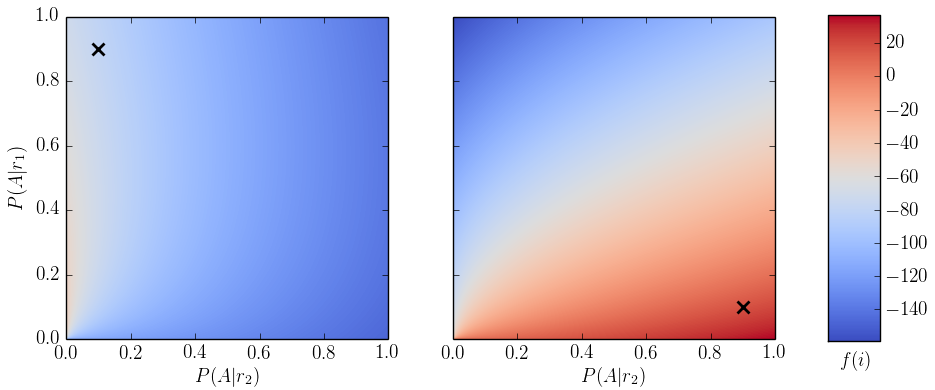
\includegraphics[width=\textwidth]{objective_function_cropped.png}
\scalebox{.65}{%% Creator: Matplotlib, PGF backend
%%
%% To include the figure in your LaTeX document, write
%%   \input{<filename>.pgf}
%%
%% Make sure the required packages are loaded in your preamble
%%   \usepackage{pgf}
%%
%% Figures using additional raster images can only be included by \input if
%% they are in the same directory as the main LaTeX file. For loading figures
%% from other directories you can use the `import` package
%%   \usepackage{import}
%% and then include the figures with
%%   \import{<path to file>}{<filename>.pgf}
%%
%% Matplotlib used the following preamble
%%   \usepackage{fontspec}
%%   \setsansfont{DejaVu Sans}
%%   \setmonofont{DejaVu Sans Mono}
%%
\begingroup%
\makeatletter%
\begin{pgfpicture}%
\pgfpathrectangle{\pgfpointorigin}{\pgfqpoint{8.150000in}{4.250000in}}%
\pgfusepath{use as bounding box, clip}%
\begin{pgfscope}%
\pgfsetbuttcap%
\pgfsetmiterjoin%
\definecolor{currentfill}{rgb}{1.000000,1.000000,1.000000}%
\pgfsetfillcolor{currentfill}%
\pgfsetlinewidth{0.000000pt}%
\definecolor{currentstroke}{rgb}{1.000000,1.000000,1.000000}%
\pgfsetstrokecolor{currentstroke}%
\pgfsetdash{}{0pt}%
\pgfpathmoveto{\pgfqpoint{0.000000in}{0.000000in}}%
\pgfpathlineto{\pgfqpoint{8.150000in}{0.000000in}}%
\pgfpathlineto{\pgfqpoint{8.150000in}{4.250000in}}%
\pgfpathlineto{\pgfqpoint{0.000000in}{4.250000in}}%
\pgfpathclose%
\pgfusepath{fill}%
\end{pgfscope}%
\begin{pgfscope}%
\pgfsetbuttcap%
\pgfsetmiterjoin%
\definecolor{currentfill}{rgb}{1.000000,1.000000,1.000000}%
\pgfsetfillcolor{currentfill}%
\pgfsetlinewidth{0.000000pt}%
\definecolor{currentstroke}{rgb}{0.000000,0.000000,0.000000}%
\pgfsetstrokecolor{currentstroke}%
\pgfsetstrokeopacity{0.000000}%
\pgfsetdash{}{0pt}%
\pgfpathmoveto{\pgfqpoint{1.018750in}{0.425000in}}%
\pgfpathlineto{\pgfqpoint{7.335000in}{0.425000in}}%
\pgfpathlineto{\pgfqpoint{7.335000in}{3.825000in}}%
\pgfpathlineto{\pgfqpoint{1.018750in}{3.825000in}}%
\pgfpathclose%
\pgfusepath{fill}%
\end{pgfscope}%
\begin{pgfscope}%
\pgfpathrectangle{\pgfqpoint{1.018750in}{0.425000in}}{\pgfqpoint{6.316250in}{3.400000in}} %
\pgfusepath{clip}%
\pgfsetrectcap%
\pgfsetroundjoin%
\pgfsetlinewidth{1.003750pt}%
\definecolor{currentstroke}{rgb}{0.000000,0.000000,1.000000}%
\pgfsetstrokecolor{currentstroke}%
\pgfsetdash{}{0pt}%
\pgfpathmoveto{\pgfqpoint{1.755646in}{0.569747in}}%
\pgfpathlineto{\pgfqpoint{2.387271in}{0.569747in}}%
\pgfpathlineto{\pgfqpoint{2.387271in}{1.136414in}}%
\pgfpathlineto{\pgfqpoint{1.755646in}{1.136414in}}%
\pgfpathlineto{\pgfqpoint{1.755646in}{0.569747in}}%
\pgfusepath{stroke}%
\end{pgfscope}%
\begin{pgfscope}%
\pgfpathrectangle{\pgfqpoint{1.018750in}{0.425000in}}{\pgfqpoint{6.316250in}{3.400000in}} %
\pgfusepath{clip}%
\pgfsetbuttcap%
\pgfsetroundjoin%
\pgfsetlinewidth{1.003750pt}%
\definecolor{currentstroke}{rgb}{0.000000,0.000000,1.000000}%
\pgfsetstrokecolor{currentstroke}%
\pgfsetdash{{6.000000pt}{6.000000pt}}{0.000000pt}%
\pgfpathmoveto{\pgfqpoint{2.071458in}{0.569747in}}%
\pgfpathlineto{\pgfqpoint{2.071458in}{0.533560in}}%
\pgfusepath{stroke}%
\end{pgfscope}%
\begin{pgfscope}%
\pgfpathrectangle{\pgfqpoint{1.018750in}{0.425000in}}{\pgfqpoint{6.316250in}{3.400000in}} %
\pgfusepath{clip}%
\pgfsetbuttcap%
\pgfsetroundjoin%
\pgfsetlinewidth{1.003750pt}%
\definecolor{currentstroke}{rgb}{0.000000,0.000000,1.000000}%
\pgfsetstrokecolor{currentstroke}%
\pgfsetdash{{6.000000pt}{6.000000pt}}{0.000000pt}%
\pgfpathmoveto{\pgfqpoint{2.071458in}{1.136414in}}%
\pgfpathlineto{\pgfqpoint{2.071458in}{1.964343in}}%
\pgfusepath{stroke}%
\end{pgfscope}%
\begin{pgfscope}%
\pgfpathrectangle{\pgfqpoint{1.018750in}{0.425000in}}{\pgfqpoint{6.316250in}{3.400000in}} %
\pgfusepath{clip}%
\pgfsetrectcap%
\pgfsetroundjoin%
\pgfsetlinewidth{1.003750pt}%
\definecolor{currentstroke}{rgb}{0.000000,0.000000,0.000000}%
\pgfsetstrokecolor{currentstroke}%
\pgfsetdash{}{0pt}%
\pgfpathmoveto{\pgfqpoint{1.913552in}{0.533560in}}%
\pgfpathlineto{\pgfqpoint{2.229365in}{0.533560in}}%
\pgfusepath{stroke}%
\end{pgfscope}%
\begin{pgfscope}%
\pgfpathrectangle{\pgfqpoint{1.018750in}{0.425000in}}{\pgfqpoint{6.316250in}{3.400000in}} %
\pgfusepath{clip}%
\pgfsetrectcap%
\pgfsetroundjoin%
\pgfsetlinewidth{1.003750pt}%
\definecolor{currentstroke}{rgb}{0.000000,0.000000,0.000000}%
\pgfsetstrokecolor{currentstroke}%
\pgfsetdash{}{0pt}%
\pgfpathmoveto{\pgfqpoint{1.913552in}{1.964343in}}%
\pgfpathlineto{\pgfqpoint{2.229365in}{1.964343in}}%
\pgfusepath{stroke}%
\end{pgfscope}%
\begin{pgfscope}%
\pgfpathrectangle{\pgfqpoint{1.018750in}{0.425000in}}{\pgfqpoint{6.316250in}{3.400000in}} %
\pgfusepath{clip}%
\pgfsetrectcap%
\pgfsetroundjoin%
\pgfsetlinewidth{1.003750pt}%
\definecolor{currentstroke}{rgb}{1.000000,0.000000,0.000000}%
\pgfsetstrokecolor{currentstroke}%
\pgfsetdash{}{0pt}%
\pgfpathmoveto{\pgfqpoint{1.755646in}{0.947525in}}%
\pgfpathlineto{\pgfqpoint{2.387271in}{0.947525in}}%
\pgfusepath{stroke}%
\end{pgfscope}%
\begin{pgfscope}%
\pgfpathrectangle{\pgfqpoint{1.018750in}{0.425000in}}{\pgfqpoint{6.316250in}{3.400000in}} %
\pgfusepath{clip}%
\pgfsetrectcap%
\pgfsetroundjoin%
\pgfsetlinewidth{1.003750pt}%
\definecolor{currentstroke}{rgb}{0.000000,0.000000,1.000000}%
\pgfsetstrokecolor{currentstroke}%
\pgfsetdash{}{0pt}%
\pgfpathmoveto{\pgfqpoint{3.861063in}{1.369444in}}%
\pgfpathlineto{\pgfqpoint{4.492687in}{1.369444in}}%
\pgfpathlineto{\pgfqpoint{4.492687in}{2.911393in}}%
\pgfpathlineto{\pgfqpoint{3.861063in}{2.911393in}}%
\pgfpathlineto{\pgfqpoint{3.861063in}{1.369444in}}%
\pgfusepath{stroke}%
\end{pgfscope}%
\begin{pgfscope}%
\pgfpathrectangle{\pgfqpoint{1.018750in}{0.425000in}}{\pgfqpoint{6.316250in}{3.400000in}} %
\pgfusepath{clip}%
\pgfsetbuttcap%
\pgfsetroundjoin%
\pgfsetlinewidth{1.003750pt}%
\definecolor{currentstroke}{rgb}{0.000000,0.000000,1.000000}%
\pgfsetstrokecolor{currentstroke}%
\pgfsetdash{{6.000000pt}{6.000000pt}}{0.000000pt}%
\pgfpathmoveto{\pgfqpoint{4.176875in}{1.369444in}}%
\pgfpathlineto{\pgfqpoint{4.176875in}{1.369444in}}%
\pgfusepath{stroke}%
\end{pgfscope}%
\begin{pgfscope}%
\pgfpathrectangle{\pgfqpoint{1.018750in}{0.425000in}}{\pgfqpoint{6.316250in}{3.400000in}} %
\pgfusepath{clip}%
\pgfsetbuttcap%
\pgfsetroundjoin%
\pgfsetlinewidth{1.003750pt}%
\definecolor{currentstroke}{rgb}{0.000000,0.000000,1.000000}%
\pgfsetstrokecolor{currentstroke}%
\pgfsetdash{{6.000000pt}{6.000000pt}}{0.000000pt}%
\pgfpathmoveto{\pgfqpoint{4.176875in}{2.911393in}}%
\pgfpathlineto{\pgfqpoint{4.176875in}{3.478059in}}%
\pgfusepath{stroke}%
\end{pgfscope}%
\begin{pgfscope}%
\pgfpathrectangle{\pgfqpoint{1.018750in}{0.425000in}}{\pgfqpoint{6.316250in}{3.400000in}} %
\pgfusepath{clip}%
\pgfsetrectcap%
\pgfsetroundjoin%
\pgfsetlinewidth{1.003750pt}%
\definecolor{currentstroke}{rgb}{0.000000,0.000000,0.000000}%
\pgfsetstrokecolor{currentstroke}%
\pgfsetdash{}{0pt}%
\pgfpathmoveto{\pgfqpoint{4.018969in}{1.369444in}}%
\pgfpathlineto{\pgfqpoint{4.334781in}{1.369444in}}%
\pgfusepath{stroke}%
\end{pgfscope}%
\begin{pgfscope}%
\pgfpathrectangle{\pgfqpoint{1.018750in}{0.425000in}}{\pgfqpoint{6.316250in}{3.400000in}} %
\pgfusepath{clip}%
\pgfsetrectcap%
\pgfsetroundjoin%
\pgfsetlinewidth{1.003750pt}%
\definecolor{currentstroke}{rgb}{0.000000,0.000000,0.000000}%
\pgfsetstrokecolor{currentstroke}%
\pgfsetdash{}{0pt}%
\pgfpathmoveto{\pgfqpoint{4.018969in}{3.478059in}}%
\pgfpathlineto{\pgfqpoint{4.334781in}{3.478059in}}%
\pgfusepath{stroke}%
\end{pgfscope}%
\begin{pgfscope}%
\pgfpathrectangle{\pgfqpoint{1.018750in}{0.425000in}}{\pgfqpoint{6.316250in}{3.400000in}} %
\pgfusepath{clip}%
\pgfsetrectcap%
\pgfsetroundjoin%
\pgfsetlinewidth{1.003750pt}%
\definecolor{currentstroke}{rgb}{1.000000,0.000000,0.000000}%
\pgfsetstrokecolor{currentstroke}%
\pgfsetdash{}{0pt}%
\pgfpathmoveto{\pgfqpoint{3.861063in}{1.558333in}}%
\pgfpathlineto{\pgfqpoint{4.492687in}{1.558333in}}%
\pgfusepath{stroke}%
\end{pgfscope}%
\begin{pgfscope}%
\pgfpathrectangle{\pgfqpoint{1.018750in}{0.425000in}}{\pgfqpoint{6.316250in}{3.400000in}} %
\pgfusepath{clip}%
\pgfsetrectcap%
\pgfsetroundjoin%
\pgfsetlinewidth{1.003750pt}%
\definecolor{currentstroke}{rgb}{0.000000,0.000000,1.000000}%
\pgfsetstrokecolor{currentstroke}%
\pgfsetdash{}{0pt}%
\pgfpathmoveto{\pgfqpoint{5.966479in}{1.369444in}}%
\pgfpathlineto{\pgfqpoint{6.598104in}{1.369444in}}%
\pgfpathlineto{\pgfqpoint{6.598104in}{1.621195in}}%
\pgfpathlineto{\pgfqpoint{5.966479in}{1.621195in}}%
\pgfpathlineto{\pgfqpoint{5.966479in}{1.369444in}}%
\pgfusepath{stroke}%
\end{pgfscope}%
\begin{pgfscope}%
\pgfpathrectangle{\pgfqpoint{1.018750in}{0.425000in}}{\pgfqpoint{6.316250in}{3.400000in}} %
\pgfusepath{clip}%
\pgfsetbuttcap%
\pgfsetroundjoin%
\pgfsetlinewidth{1.003750pt}%
\definecolor{currentstroke}{rgb}{0.000000,0.000000,1.000000}%
\pgfsetstrokecolor{currentstroke}%
\pgfsetdash{{6.000000pt}{6.000000pt}}{0.000000pt}%
\pgfpathmoveto{\pgfqpoint{6.282292in}{1.369444in}}%
\pgfpathlineto{\pgfqpoint{6.282292in}{1.054529in}}%
\pgfusepath{stroke}%
\end{pgfscope}%
\begin{pgfscope}%
\pgfpathrectangle{\pgfqpoint{1.018750in}{0.425000in}}{\pgfqpoint{6.316250in}{3.400000in}} %
\pgfusepath{clip}%
\pgfsetbuttcap%
\pgfsetroundjoin%
\pgfsetlinewidth{1.003750pt}%
\definecolor{currentstroke}{rgb}{0.000000,0.000000,1.000000}%
\pgfsetstrokecolor{currentstroke}%
\pgfsetdash{{6.000000pt}{6.000000pt}}{0.000000pt}%
\pgfpathmoveto{\pgfqpoint{6.282292in}{1.621195in}}%
\pgfpathlineto{\pgfqpoint{6.282292in}{1.936111in}}%
\pgfusepath{stroke}%
\end{pgfscope}%
\begin{pgfscope}%
\pgfpathrectangle{\pgfqpoint{1.018750in}{0.425000in}}{\pgfqpoint{6.316250in}{3.400000in}} %
\pgfusepath{clip}%
\pgfsetrectcap%
\pgfsetroundjoin%
\pgfsetlinewidth{1.003750pt}%
\definecolor{currentstroke}{rgb}{0.000000,0.000000,0.000000}%
\pgfsetstrokecolor{currentstroke}%
\pgfsetdash{}{0pt}%
\pgfpathmoveto{\pgfqpoint{6.124385in}{1.054529in}}%
\pgfpathlineto{\pgfqpoint{6.440198in}{1.054529in}}%
\pgfusepath{stroke}%
\end{pgfscope}%
\begin{pgfscope}%
\pgfpathrectangle{\pgfqpoint{1.018750in}{0.425000in}}{\pgfqpoint{6.316250in}{3.400000in}} %
\pgfusepath{clip}%
\pgfsetrectcap%
\pgfsetroundjoin%
\pgfsetlinewidth{1.003750pt}%
\definecolor{currentstroke}{rgb}{0.000000,0.000000,0.000000}%
\pgfsetstrokecolor{currentstroke}%
\pgfsetdash{}{0pt}%
\pgfpathmoveto{\pgfqpoint{6.124385in}{1.936111in}}%
\pgfpathlineto{\pgfqpoint{6.440198in}{1.936111in}}%
\pgfusepath{stroke}%
\end{pgfscope}%
\begin{pgfscope}%
\pgfpathrectangle{\pgfqpoint{1.018750in}{0.425000in}}{\pgfqpoint{6.316250in}{3.400000in}} %
\pgfusepath{clip}%
\pgfsetrectcap%
\pgfsetroundjoin%
\pgfsetlinewidth{1.003750pt}%
\definecolor{currentstroke}{rgb}{1.000000,0.000000,0.000000}%
\pgfsetstrokecolor{currentstroke}%
\pgfsetdash{}{0pt}%
\pgfpathmoveto{\pgfqpoint{5.966479in}{1.558333in}}%
\pgfpathlineto{\pgfqpoint{6.598104in}{1.558333in}}%
\pgfusepath{stroke}%
\end{pgfscope}%
\begin{pgfscope}%
\pgfsetrectcap%
\pgfsetmiterjoin%
\pgfsetlinewidth{1.003750pt}%
\definecolor{currentstroke}{rgb}{0.000000,0.000000,0.000000}%
\pgfsetstrokecolor{currentstroke}%
\pgfsetdash{}{0pt}%
\pgfpathmoveto{\pgfqpoint{1.018750in}{3.825000in}}%
\pgfpathlineto{\pgfqpoint{7.335000in}{3.825000in}}%
\pgfusepath{stroke}%
\end{pgfscope}%
\begin{pgfscope}%
\pgfsetrectcap%
\pgfsetmiterjoin%
\pgfsetlinewidth{1.003750pt}%
\definecolor{currentstroke}{rgb}{0.000000,0.000000,0.000000}%
\pgfsetstrokecolor{currentstroke}%
\pgfsetdash{}{0pt}%
\pgfpathmoveto{\pgfqpoint{7.335000in}{0.425000in}}%
\pgfpathlineto{\pgfqpoint{7.335000in}{3.825000in}}%
\pgfusepath{stroke}%
\end{pgfscope}%
\begin{pgfscope}%
\pgfsetrectcap%
\pgfsetmiterjoin%
\pgfsetlinewidth{1.003750pt}%
\definecolor{currentstroke}{rgb}{0.000000,0.000000,0.000000}%
\pgfsetstrokecolor{currentstroke}%
\pgfsetdash{}{0pt}%
\pgfpathmoveto{\pgfqpoint{1.018750in}{0.425000in}}%
\pgfpathlineto{\pgfqpoint{7.335000in}{0.425000in}}%
\pgfusepath{stroke}%
\end{pgfscope}%
\begin{pgfscope}%
\pgfsetrectcap%
\pgfsetmiterjoin%
\pgfsetlinewidth{1.003750pt}%
\definecolor{currentstroke}{rgb}{0.000000,0.000000,0.000000}%
\pgfsetstrokecolor{currentstroke}%
\pgfsetdash{}{0pt}%
\pgfpathmoveto{\pgfqpoint{1.018750in}{0.425000in}}%
\pgfpathlineto{\pgfqpoint{1.018750in}{3.825000in}}%
\pgfusepath{stroke}%
\end{pgfscope}%
\begin{pgfscope}%
\pgfsetbuttcap%
\pgfsetroundjoin%
\definecolor{currentfill}{rgb}{0.000000,0.000000,0.000000}%
\pgfsetfillcolor{currentfill}%
\pgfsetlinewidth{0.501875pt}%
\definecolor{currentstroke}{rgb}{0.000000,0.000000,0.000000}%
\pgfsetstrokecolor{currentstroke}%
\pgfsetdash{}{0pt}%
\pgfsys@defobject{currentmarker}{\pgfqpoint{0.000000in}{0.000000in}}{\pgfqpoint{0.000000in}{0.055556in}}{%
\pgfpathmoveto{\pgfqpoint{0.000000in}{0.000000in}}%
\pgfpathlineto{\pgfqpoint{0.000000in}{0.055556in}}%
\pgfusepath{stroke,fill}%
}%
\begin{pgfscope}%
\pgfsys@transformshift{2.071458in}{0.425000in}%
\pgfsys@useobject{currentmarker}{}%
\end{pgfscope}%
\end{pgfscope}%
\begin{pgfscope}%
\pgfsetbuttcap%
\pgfsetroundjoin%
\definecolor{currentfill}{rgb}{0.000000,0.000000,0.000000}%
\pgfsetfillcolor{currentfill}%
\pgfsetlinewidth{0.501875pt}%
\definecolor{currentstroke}{rgb}{0.000000,0.000000,0.000000}%
\pgfsetstrokecolor{currentstroke}%
\pgfsetdash{}{0pt}%
\pgfsys@defobject{currentmarker}{\pgfqpoint{0.000000in}{-0.055556in}}{\pgfqpoint{0.000000in}{0.000000in}}{%
\pgfpathmoveto{\pgfqpoint{0.000000in}{0.000000in}}%
\pgfpathlineto{\pgfqpoint{0.000000in}{-0.055556in}}%
\pgfusepath{stroke,fill}%
}%
\begin{pgfscope}%
\pgfsys@transformshift{2.071458in}{3.825000in}%
\pgfsys@useobject{currentmarker}{}%
\end{pgfscope}%
\end{pgfscope}%
\begin{pgfscope}%
\pgftext[x=2.071458in,y=0.369444in,,top]{{\sffamily\fontsize{14.000000}{16.800000}\selectfont \textrm{Repair model}}}%
\end{pgfscope}%
\begin{pgfscope}%
\pgfsetbuttcap%
\pgfsetroundjoin%
\definecolor{currentfill}{rgb}{0.000000,0.000000,0.000000}%
\pgfsetfillcolor{currentfill}%
\pgfsetlinewidth{0.501875pt}%
\definecolor{currentstroke}{rgb}{0.000000,0.000000,0.000000}%
\pgfsetstrokecolor{currentstroke}%
\pgfsetdash{}{0pt}%
\pgfsys@defobject{currentmarker}{\pgfqpoint{0.000000in}{0.000000in}}{\pgfqpoint{0.000000in}{0.055556in}}{%
\pgfpathmoveto{\pgfqpoint{0.000000in}{0.000000in}}%
\pgfpathlineto{\pgfqpoint{0.000000in}{0.055556in}}%
\pgfusepath{stroke,fill}%
}%
\begin{pgfscope}%
\pgfsys@transformshift{4.176875in}{0.425000in}%
\pgfsys@useobject{currentmarker}{}%
\end{pgfscope}%
\end{pgfscope}%
\begin{pgfscope}%
\pgfsetbuttcap%
\pgfsetroundjoin%
\definecolor{currentfill}{rgb}{0.000000,0.000000,0.000000}%
\pgfsetfillcolor{currentfill}%
\pgfsetlinewidth{0.501875pt}%
\definecolor{currentstroke}{rgb}{0.000000,0.000000,0.000000}%
\pgfsetstrokecolor{currentstroke}%
\pgfsetdash{}{0pt}%
\pgfsys@defobject{currentmarker}{\pgfqpoint{0.000000in}{-0.055556in}}{\pgfqpoint{0.000000in}{0.000000in}}{%
\pgfpathmoveto{\pgfqpoint{0.000000in}{0.000000in}}%
\pgfpathlineto{\pgfqpoint{0.000000in}{-0.055556in}}%
\pgfusepath{stroke,fill}%
}%
\begin{pgfscope}%
\pgfsys@transformshift{4.176875in}{3.825000in}%
\pgfsys@useobject{currentmarker}{}%
\end{pgfscope}%
\end{pgfscope}%
\begin{pgfscope}%
\pgftext[x=4.176875in,y=0.369444in,,top]{{\sffamily\fontsize{14.000000}{16.800000}\selectfont \textrm{Rejection model}}}%
\end{pgfscope}%
\begin{pgfscope}%
\pgfsetbuttcap%
\pgfsetroundjoin%
\definecolor{currentfill}{rgb}{0.000000,0.000000,0.000000}%
\pgfsetfillcolor{currentfill}%
\pgfsetlinewidth{0.501875pt}%
\definecolor{currentstroke}{rgb}{0.000000,0.000000,0.000000}%
\pgfsetstrokecolor{currentstroke}%
\pgfsetdash{}{0pt}%
\pgfsys@defobject{currentmarker}{\pgfqpoint{0.000000in}{0.000000in}}{\pgfqpoint{0.000000in}{0.055556in}}{%
\pgfpathmoveto{\pgfqpoint{0.000000in}{0.000000in}}%
\pgfpathlineto{\pgfqpoint{0.000000in}{0.055556in}}%
\pgfusepath{stroke,fill}%
}%
\begin{pgfscope}%
\pgfsys@transformshift{6.282292in}{0.425000in}%
\pgfsys@useobject{currentmarker}{}%
\end{pgfscope}%
\end{pgfscope}%
\begin{pgfscope}%
\pgfsetbuttcap%
\pgfsetroundjoin%
\definecolor{currentfill}{rgb}{0.000000,0.000000,0.000000}%
\pgfsetfillcolor{currentfill}%
\pgfsetlinewidth{0.501875pt}%
\definecolor{currentstroke}{rgb}{0.000000,0.000000,0.000000}%
\pgfsetstrokecolor{currentstroke}%
\pgfsetdash{}{0pt}%
\pgfsys@defobject{currentmarker}{\pgfqpoint{0.000000in}{-0.055556in}}{\pgfqpoint{0.000000in}{0.000000in}}{%
\pgfpathmoveto{\pgfqpoint{0.000000in}{0.000000in}}%
\pgfpathlineto{\pgfqpoint{0.000000in}{-0.055556in}}%
\pgfusepath{stroke,fill}%
}%
\begin{pgfscope}%
\pgfsys@transformshift{6.282292in}{3.825000in}%
\pgfsys@useobject{currentmarker}{}%
\end{pgfscope}%
\end{pgfscope}%
\begin{pgfscope}%
\pgftext[x=6.282292in,y=0.369444in,,top]{{\sffamily\fontsize{14.000000}{16.800000}\selectfont \textrm{Baseline model}}}%
\end{pgfscope}%
\begin{pgfscope}%
\pgfsetbuttcap%
\pgfsetroundjoin%
\definecolor{currentfill}{rgb}{0.000000,0.000000,0.000000}%
\pgfsetfillcolor{currentfill}%
\pgfsetlinewidth{0.501875pt}%
\definecolor{currentstroke}{rgb}{0.000000,0.000000,0.000000}%
\pgfsetstrokecolor{currentstroke}%
\pgfsetdash{}{0pt}%
\pgfsys@defobject{currentmarker}{\pgfqpoint{0.000000in}{0.000000in}}{\pgfqpoint{0.055556in}{0.000000in}}{%
\pgfpathmoveto{\pgfqpoint{0.000000in}{0.000000in}}%
\pgfpathlineto{\pgfqpoint{0.055556in}{0.000000in}}%
\pgfusepath{stroke,fill}%
}%
\begin{pgfscope}%
\pgfsys@transformshift{1.018750in}{0.425000in}%
\pgfsys@useobject{currentmarker}{}%
\end{pgfscope}%
\end{pgfscope}%
\begin{pgfscope}%
\pgfsetbuttcap%
\pgfsetroundjoin%
\definecolor{currentfill}{rgb}{0.000000,0.000000,0.000000}%
\pgfsetfillcolor{currentfill}%
\pgfsetlinewidth{0.501875pt}%
\definecolor{currentstroke}{rgb}{0.000000,0.000000,0.000000}%
\pgfsetstrokecolor{currentstroke}%
\pgfsetdash{}{0pt}%
\pgfsys@defobject{currentmarker}{\pgfqpoint{-0.055556in}{0.000000in}}{\pgfqpoint{0.000000in}{0.000000in}}{%
\pgfpathmoveto{\pgfqpoint{0.000000in}{0.000000in}}%
\pgfpathlineto{\pgfqpoint{-0.055556in}{0.000000in}}%
\pgfusepath{stroke,fill}%
}%
\begin{pgfscope}%
\pgfsys@transformshift{7.335000in}{0.425000in}%
\pgfsys@useobject{currentmarker}{}%
\end{pgfscope}%
\end{pgfscope}%
\begin{pgfscope}%
\pgftext[x=0.963194in,y=0.425000in,right,]{{\sffamily\fontsize{14.000000}{16.800000}\selectfont \(\displaystyle 0.0\)}}%
\end{pgfscope}%
\begin{pgfscope}%
\pgfsetbuttcap%
\pgfsetroundjoin%
\definecolor{currentfill}{rgb}{0.000000,0.000000,0.000000}%
\pgfsetfillcolor{currentfill}%
\pgfsetlinewidth{0.501875pt}%
\definecolor{currentstroke}{rgb}{0.000000,0.000000,0.000000}%
\pgfsetstrokecolor{currentstroke}%
\pgfsetdash{}{0pt}%
\pgfsys@defobject{currentmarker}{\pgfqpoint{0.000000in}{0.000000in}}{\pgfqpoint{0.055556in}{0.000000in}}{%
\pgfpathmoveto{\pgfqpoint{0.000000in}{0.000000in}}%
\pgfpathlineto{\pgfqpoint{0.055556in}{0.000000in}}%
\pgfusepath{stroke,fill}%
}%
\begin{pgfscope}%
\pgfsys@transformshift{1.018750in}{0.802778in}%
\pgfsys@useobject{currentmarker}{}%
\end{pgfscope}%
\end{pgfscope}%
\begin{pgfscope}%
\pgfsetbuttcap%
\pgfsetroundjoin%
\definecolor{currentfill}{rgb}{0.000000,0.000000,0.000000}%
\pgfsetfillcolor{currentfill}%
\pgfsetlinewidth{0.501875pt}%
\definecolor{currentstroke}{rgb}{0.000000,0.000000,0.000000}%
\pgfsetstrokecolor{currentstroke}%
\pgfsetdash{}{0pt}%
\pgfsys@defobject{currentmarker}{\pgfqpoint{-0.055556in}{0.000000in}}{\pgfqpoint{0.000000in}{0.000000in}}{%
\pgfpathmoveto{\pgfqpoint{0.000000in}{0.000000in}}%
\pgfpathlineto{\pgfqpoint{-0.055556in}{0.000000in}}%
\pgfusepath{stroke,fill}%
}%
\begin{pgfscope}%
\pgfsys@transformshift{7.335000in}{0.802778in}%
\pgfsys@useobject{currentmarker}{}%
\end{pgfscope}%
\end{pgfscope}%
\begin{pgfscope}%
\pgftext[x=0.963194in,y=0.802778in,right,]{{\sffamily\fontsize{14.000000}{16.800000}\selectfont \(\displaystyle 0.2\)}}%
\end{pgfscope}%
\begin{pgfscope}%
\pgfsetbuttcap%
\pgfsetroundjoin%
\definecolor{currentfill}{rgb}{0.000000,0.000000,0.000000}%
\pgfsetfillcolor{currentfill}%
\pgfsetlinewidth{0.501875pt}%
\definecolor{currentstroke}{rgb}{0.000000,0.000000,0.000000}%
\pgfsetstrokecolor{currentstroke}%
\pgfsetdash{}{0pt}%
\pgfsys@defobject{currentmarker}{\pgfqpoint{0.000000in}{0.000000in}}{\pgfqpoint{0.055556in}{0.000000in}}{%
\pgfpathmoveto{\pgfqpoint{0.000000in}{0.000000in}}%
\pgfpathlineto{\pgfqpoint{0.055556in}{0.000000in}}%
\pgfusepath{stroke,fill}%
}%
\begin{pgfscope}%
\pgfsys@transformshift{1.018750in}{1.180556in}%
\pgfsys@useobject{currentmarker}{}%
\end{pgfscope}%
\end{pgfscope}%
\begin{pgfscope}%
\pgfsetbuttcap%
\pgfsetroundjoin%
\definecolor{currentfill}{rgb}{0.000000,0.000000,0.000000}%
\pgfsetfillcolor{currentfill}%
\pgfsetlinewidth{0.501875pt}%
\definecolor{currentstroke}{rgb}{0.000000,0.000000,0.000000}%
\pgfsetstrokecolor{currentstroke}%
\pgfsetdash{}{0pt}%
\pgfsys@defobject{currentmarker}{\pgfqpoint{-0.055556in}{0.000000in}}{\pgfqpoint{0.000000in}{0.000000in}}{%
\pgfpathmoveto{\pgfqpoint{0.000000in}{0.000000in}}%
\pgfpathlineto{\pgfqpoint{-0.055556in}{0.000000in}}%
\pgfusepath{stroke,fill}%
}%
\begin{pgfscope}%
\pgfsys@transformshift{7.335000in}{1.180556in}%
\pgfsys@useobject{currentmarker}{}%
\end{pgfscope}%
\end{pgfscope}%
\begin{pgfscope}%
\pgftext[x=0.963194in,y=1.180556in,right,]{{\sffamily\fontsize{14.000000}{16.800000}\selectfont \(\displaystyle 0.4\)}}%
\end{pgfscope}%
\begin{pgfscope}%
\pgfsetbuttcap%
\pgfsetroundjoin%
\definecolor{currentfill}{rgb}{0.000000,0.000000,0.000000}%
\pgfsetfillcolor{currentfill}%
\pgfsetlinewidth{0.501875pt}%
\definecolor{currentstroke}{rgb}{0.000000,0.000000,0.000000}%
\pgfsetstrokecolor{currentstroke}%
\pgfsetdash{}{0pt}%
\pgfsys@defobject{currentmarker}{\pgfqpoint{0.000000in}{0.000000in}}{\pgfqpoint{0.055556in}{0.000000in}}{%
\pgfpathmoveto{\pgfqpoint{0.000000in}{0.000000in}}%
\pgfpathlineto{\pgfqpoint{0.055556in}{0.000000in}}%
\pgfusepath{stroke,fill}%
}%
\begin{pgfscope}%
\pgfsys@transformshift{1.018750in}{1.558333in}%
\pgfsys@useobject{currentmarker}{}%
\end{pgfscope}%
\end{pgfscope}%
\begin{pgfscope}%
\pgfsetbuttcap%
\pgfsetroundjoin%
\definecolor{currentfill}{rgb}{0.000000,0.000000,0.000000}%
\pgfsetfillcolor{currentfill}%
\pgfsetlinewidth{0.501875pt}%
\definecolor{currentstroke}{rgb}{0.000000,0.000000,0.000000}%
\pgfsetstrokecolor{currentstroke}%
\pgfsetdash{}{0pt}%
\pgfsys@defobject{currentmarker}{\pgfqpoint{-0.055556in}{0.000000in}}{\pgfqpoint{0.000000in}{0.000000in}}{%
\pgfpathmoveto{\pgfqpoint{0.000000in}{0.000000in}}%
\pgfpathlineto{\pgfqpoint{-0.055556in}{0.000000in}}%
\pgfusepath{stroke,fill}%
}%
\begin{pgfscope}%
\pgfsys@transformshift{7.335000in}{1.558333in}%
\pgfsys@useobject{currentmarker}{}%
\end{pgfscope}%
\end{pgfscope}%
\begin{pgfscope}%
\pgftext[x=0.963194in,y=1.558333in,right,]{{\sffamily\fontsize{14.000000}{16.800000}\selectfont \(\displaystyle 0.6\)}}%
\end{pgfscope}%
\begin{pgfscope}%
\pgfsetbuttcap%
\pgfsetroundjoin%
\definecolor{currentfill}{rgb}{0.000000,0.000000,0.000000}%
\pgfsetfillcolor{currentfill}%
\pgfsetlinewidth{0.501875pt}%
\definecolor{currentstroke}{rgb}{0.000000,0.000000,0.000000}%
\pgfsetstrokecolor{currentstroke}%
\pgfsetdash{}{0pt}%
\pgfsys@defobject{currentmarker}{\pgfqpoint{0.000000in}{0.000000in}}{\pgfqpoint{0.055556in}{0.000000in}}{%
\pgfpathmoveto{\pgfqpoint{0.000000in}{0.000000in}}%
\pgfpathlineto{\pgfqpoint{0.055556in}{0.000000in}}%
\pgfusepath{stroke,fill}%
}%
\begin{pgfscope}%
\pgfsys@transformshift{1.018750in}{1.936111in}%
\pgfsys@useobject{currentmarker}{}%
\end{pgfscope}%
\end{pgfscope}%
\begin{pgfscope}%
\pgfsetbuttcap%
\pgfsetroundjoin%
\definecolor{currentfill}{rgb}{0.000000,0.000000,0.000000}%
\pgfsetfillcolor{currentfill}%
\pgfsetlinewidth{0.501875pt}%
\definecolor{currentstroke}{rgb}{0.000000,0.000000,0.000000}%
\pgfsetstrokecolor{currentstroke}%
\pgfsetdash{}{0pt}%
\pgfsys@defobject{currentmarker}{\pgfqpoint{-0.055556in}{0.000000in}}{\pgfqpoint{0.000000in}{0.000000in}}{%
\pgfpathmoveto{\pgfqpoint{0.000000in}{0.000000in}}%
\pgfpathlineto{\pgfqpoint{-0.055556in}{0.000000in}}%
\pgfusepath{stroke,fill}%
}%
\begin{pgfscope}%
\pgfsys@transformshift{7.335000in}{1.936111in}%
\pgfsys@useobject{currentmarker}{}%
\end{pgfscope}%
\end{pgfscope}%
\begin{pgfscope}%
\pgftext[x=0.963194in,y=1.936111in,right,]{{\sffamily\fontsize{14.000000}{16.800000}\selectfont \(\displaystyle 0.8\)}}%
\end{pgfscope}%
\begin{pgfscope}%
\pgfsetbuttcap%
\pgfsetroundjoin%
\definecolor{currentfill}{rgb}{0.000000,0.000000,0.000000}%
\pgfsetfillcolor{currentfill}%
\pgfsetlinewidth{0.501875pt}%
\definecolor{currentstroke}{rgb}{0.000000,0.000000,0.000000}%
\pgfsetstrokecolor{currentstroke}%
\pgfsetdash{}{0pt}%
\pgfsys@defobject{currentmarker}{\pgfqpoint{0.000000in}{0.000000in}}{\pgfqpoint{0.055556in}{0.000000in}}{%
\pgfpathmoveto{\pgfqpoint{0.000000in}{0.000000in}}%
\pgfpathlineto{\pgfqpoint{0.055556in}{0.000000in}}%
\pgfusepath{stroke,fill}%
}%
\begin{pgfscope}%
\pgfsys@transformshift{1.018750in}{2.313889in}%
\pgfsys@useobject{currentmarker}{}%
\end{pgfscope}%
\end{pgfscope}%
\begin{pgfscope}%
\pgfsetbuttcap%
\pgfsetroundjoin%
\definecolor{currentfill}{rgb}{0.000000,0.000000,0.000000}%
\pgfsetfillcolor{currentfill}%
\pgfsetlinewidth{0.501875pt}%
\definecolor{currentstroke}{rgb}{0.000000,0.000000,0.000000}%
\pgfsetstrokecolor{currentstroke}%
\pgfsetdash{}{0pt}%
\pgfsys@defobject{currentmarker}{\pgfqpoint{-0.055556in}{0.000000in}}{\pgfqpoint{0.000000in}{0.000000in}}{%
\pgfpathmoveto{\pgfqpoint{0.000000in}{0.000000in}}%
\pgfpathlineto{\pgfqpoint{-0.055556in}{0.000000in}}%
\pgfusepath{stroke,fill}%
}%
\begin{pgfscope}%
\pgfsys@transformshift{7.335000in}{2.313889in}%
\pgfsys@useobject{currentmarker}{}%
\end{pgfscope}%
\end{pgfscope}%
\begin{pgfscope}%
\pgftext[x=0.963194in,y=2.313889in,right,]{{\sffamily\fontsize{14.000000}{16.800000}\selectfont \(\displaystyle 1.0\)}}%
\end{pgfscope}%
\begin{pgfscope}%
\pgfsetbuttcap%
\pgfsetroundjoin%
\definecolor{currentfill}{rgb}{0.000000,0.000000,0.000000}%
\pgfsetfillcolor{currentfill}%
\pgfsetlinewidth{0.501875pt}%
\definecolor{currentstroke}{rgb}{0.000000,0.000000,0.000000}%
\pgfsetstrokecolor{currentstroke}%
\pgfsetdash{}{0pt}%
\pgfsys@defobject{currentmarker}{\pgfqpoint{0.000000in}{0.000000in}}{\pgfqpoint{0.055556in}{0.000000in}}{%
\pgfpathmoveto{\pgfqpoint{0.000000in}{0.000000in}}%
\pgfpathlineto{\pgfqpoint{0.055556in}{0.000000in}}%
\pgfusepath{stroke,fill}%
}%
\begin{pgfscope}%
\pgfsys@transformshift{1.018750in}{2.691667in}%
\pgfsys@useobject{currentmarker}{}%
\end{pgfscope}%
\end{pgfscope}%
\begin{pgfscope}%
\pgfsetbuttcap%
\pgfsetroundjoin%
\definecolor{currentfill}{rgb}{0.000000,0.000000,0.000000}%
\pgfsetfillcolor{currentfill}%
\pgfsetlinewidth{0.501875pt}%
\definecolor{currentstroke}{rgb}{0.000000,0.000000,0.000000}%
\pgfsetstrokecolor{currentstroke}%
\pgfsetdash{}{0pt}%
\pgfsys@defobject{currentmarker}{\pgfqpoint{-0.055556in}{0.000000in}}{\pgfqpoint{0.000000in}{0.000000in}}{%
\pgfpathmoveto{\pgfqpoint{0.000000in}{0.000000in}}%
\pgfpathlineto{\pgfqpoint{-0.055556in}{0.000000in}}%
\pgfusepath{stroke,fill}%
}%
\begin{pgfscope}%
\pgfsys@transformshift{7.335000in}{2.691667in}%
\pgfsys@useobject{currentmarker}{}%
\end{pgfscope}%
\end{pgfscope}%
\begin{pgfscope}%
\pgftext[x=0.963194in,y=2.691667in,right,]{{\sffamily\fontsize{14.000000}{16.800000}\selectfont \(\displaystyle 1.2\)}}%
\end{pgfscope}%
\begin{pgfscope}%
\pgfsetbuttcap%
\pgfsetroundjoin%
\definecolor{currentfill}{rgb}{0.000000,0.000000,0.000000}%
\pgfsetfillcolor{currentfill}%
\pgfsetlinewidth{0.501875pt}%
\definecolor{currentstroke}{rgb}{0.000000,0.000000,0.000000}%
\pgfsetstrokecolor{currentstroke}%
\pgfsetdash{}{0pt}%
\pgfsys@defobject{currentmarker}{\pgfqpoint{0.000000in}{0.000000in}}{\pgfqpoint{0.055556in}{0.000000in}}{%
\pgfpathmoveto{\pgfqpoint{0.000000in}{0.000000in}}%
\pgfpathlineto{\pgfqpoint{0.055556in}{0.000000in}}%
\pgfusepath{stroke,fill}%
}%
\begin{pgfscope}%
\pgfsys@transformshift{1.018750in}{3.069444in}%
\pgfsys@useobject{currentmarker}{}%
\end{pgfscope}%
\end{pgfscope}%
\begin{pgfscope}%
\pgfsetbuttcap%
\pgfsetroundjoin%
\definecolor{currentfill}{rgb}{0.000000,0.000000,0.000000}%
\pgfsetfillcolor{currentfill}%
\pgfsetlinewidth{0.501875pt}%
\definecolor{currentstroke}{rgb}{0.000000,0.000000,0.000000}%
\pgfsetstrokecolor{currentstroke}%
\pgfsetdash{}{0pt}%
\pgfsys@defobject{currentmarker}{\pgfqpoint{-0.055556in}{0.000000in}}{\pgfqpoint{0.000000in}{0.000000in}}{%
\pgfpathmoveto{\pgfqpoint{0.000000in}{0.000000in}}%
\pgfpathlineto{\pgfqpoint{-0.055556in}{0.000000in}}%
\pgfusepath{stroke,fill}%
}%
\begin{pgfscope}%
\pgfsys@transformshift{7.335000in}{3.069444in}%
\pgfsys@useobject{currentmarker}{}%
\end{pgfscope}%
\end{pgfscope}%
\begin{pgfscope}%
\pgftext[x=0.963194in,y=3.069444in,right,]{{\sffamily\fontsize{14.000000}{16.800000}\selectfont \(\displaystyle 1.4\)}}%
\end{pgfscope}%
\begin{pgfscope}%
\pgfsetbuttcap%
\pgfsetroundjoin%
\definecolor{currentfill}{rgb}{0.000000,0.000000,0.000000}%
\pgfsetfillcolor{currentfill}%
\pgfsetlinewidth{0.501875pt}%
\definecolor{currentstroke}{rgb}{0.000000,0.000000,0.000000}%
\pgfsetstrokecolor{currentstroke}%
\pgfsetdash{}{0pt}%
\pgfsys@defobject{currentmarker}{\pgfqpoint{0.000000in}{0.000000in}}{\pgfqpoint{0.055556in}{0.000000in}}{%
\pgfpathmoveto{\pgfqpoint{0.000000in}{0.000000in}}%
\pgfpathlineto{\pgfqpoint{0.055556in}{0.000000in}}%
\pgfusepath{stroke,fill}%
}%
\begin{pgfscope}%
\pgfsys@transformshift{1.018750in}{3.447222in}%
\pgfsys@useobject{currentmarker}{}%
\end{pgfscope}%
\end{pgfscope}%
\begin{pgfscope}%
\pgfsetbuttcap%
\pgfsetroundjoin%
\definecolor{currentfill}{rgb}{0.000000,0.000000,0.000000}%
\pgfsetfillcolor{currentfill}%
\pgfsetlinewidth{0.501875pt}%
\definecolor{currentstroke}{rgb}{0.000000,0.000000,0.000000}%
\pgfsetstrokecolor{currentstroke}%
\pgfsetdash{}{0pt}%
\pgfsys@defobject{currentmarker}{\pgfqpoint{-0.055556in}{0.000000in}}{\pgfqpoint{0.000000in}{0.000000in}}{%
\pgfpathmoveto{\pgfqpoint{0.000000in}{0.000000in}}%
\pgfpathlineto{\pgfqpoint{-0.055556in}{0.000000in}}%
\pgfusepath{stroke,fill}%
}%
\begin{pgfscope}%
\pgfsys@transformshift{7.335000in}{3.447222in}%
\pgfsys@useobject{currentmarker}{}%
\end{pgfscope}%
\end{pgfscope}%
\begin{pgfscope}%
\pgftext[x=0.963194in,y=3.447222in,right,]{{\sffamily\fontsize{14.000000}{16.800000}\selectfont \(\displaystyle 1.6\)}}%
\end{pgfscope}%
\begin{pgfscope}%
\pgfsetbuttcap%
\pgfsetroundjoin%
\definecolor{currentfill}{rgb}{0.000000,0.000000,0.000000}%
\pgfsetfillcolor{currentfill}%
\pgfsetlinewidth{0.501875pt}%
\definecolor{currentstroke}{rgb}{0.000000,0.000000,0.000000}%
\pgfsetstrokecolor{currentstroke}%
\pgfsetdash{}{0pt}%
\pgfsys@defobject{currentmarker}{\pgfqpoint{0.000000in}{0.000000in}}{\pgfqpoint{0.055556in}{0.000000in}}{%
\pgfpathmoveto{\pgfqpoint{0.000000in}{0.000000in}}%
\pgfpathlineto{\pgfqpoint{0.055556in}{0.000000in}}%
\pgfusepath{stroke,fill}%
}%
\begin{pgfscope}%
\pgfsys@transformshift{1.018750in}{3.825000in}%
\pgfsys@useobject{currentmarker}{}%
\end{pgfscope}%
\end{pgfscope}%
\begin{pgfscope}%
\pgfsetbuttcap%
\pgfsetroundjoin%
\definecolor{currentfill}{rgb}{0.000000,0.000000,0.000000}%
\pgfsetfillcolor{currentfill}%
\pgfsetlinewidth{0.501875pt}%
\definecolor{currentstroke}{rgb}{0.000000,0.000000,0.000000}%
\pgfsetstrokecolor{currentstroke}%
\pgfsetdash{}{0pt}%
\pgfsys@defobject{currentmarker}{\pgfqpoint{-0.055556in}{0.000000in}}{\pgfqpoint{0.000000in}{0.000000in}}{%
\pgfpathmoveto{\pgfqpoint{0.000000in}{0.000000in}}%
\pgfpathlineto{\pgfqpoint{-0.055556in}{0.000000in}}%
\pgfusepath{stroke,fill}%
}%
\begin{pgfscope}%
\pgfsys@transformshift{7.335000in}{3.825000in}%
\pgfsys@useobject{currentmarker}{}%
\end{pgfscope}%
\end{pgfscope}%
\begin{pgfscope}%
\pgftext[x=0.963194in,y=3.825000in,right,]{{\sffamily\fontsize{14.000000}{16.800000}\selectfont \(\displaystyle 1.8\)}}%
\end{pgfscope}%
\begin{pgfscope}%
\pgftext[x=0.643522in,y=2.125000in,,bottom,rotate=90.000000]{{\sffamily\fontsize{14.000000}{16.800000}\selectfont \textrm{Error}}}%
\end{pgfscope}%
\end{pgfpicture}%
\makeatother%
\endgroup%
}
\caption{Comparison of error in scaled coordination rate across the repair, rejection and baseline models (outliers left unplotted).}
\label{fig:2}
\end{figure}

%\begin{center}
%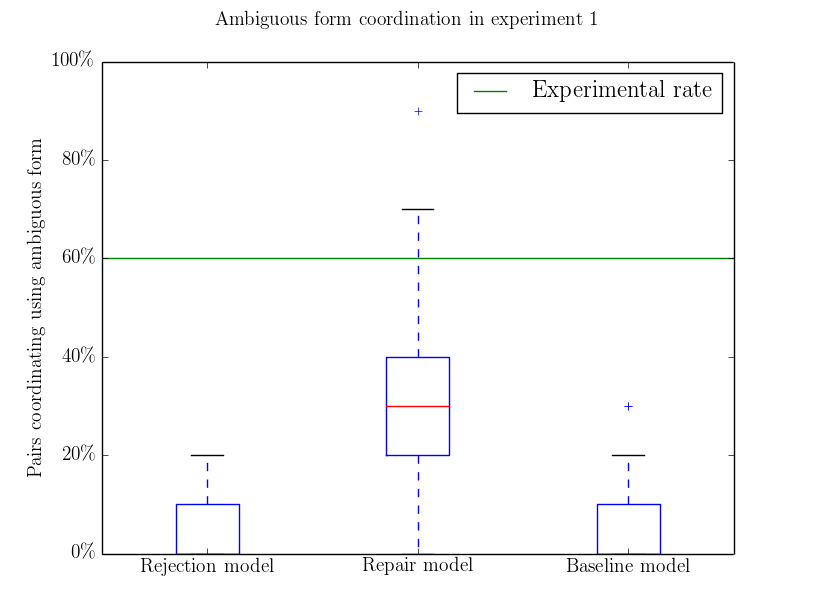
\includegraphics[width=\textwidth]{ambi_coord_exp1.png}
%\textit{Is there a more cohesive way of presenting these? Should these box/whisker plots in particular perhaps be moved to an appendix?}
%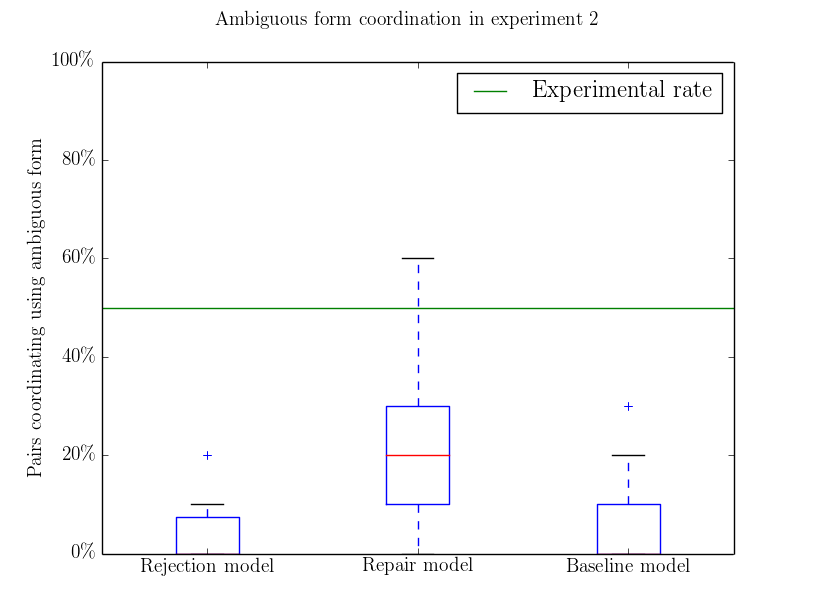
\includegraphics[width=\textwidth]{ambi_coord_exp2.png}
%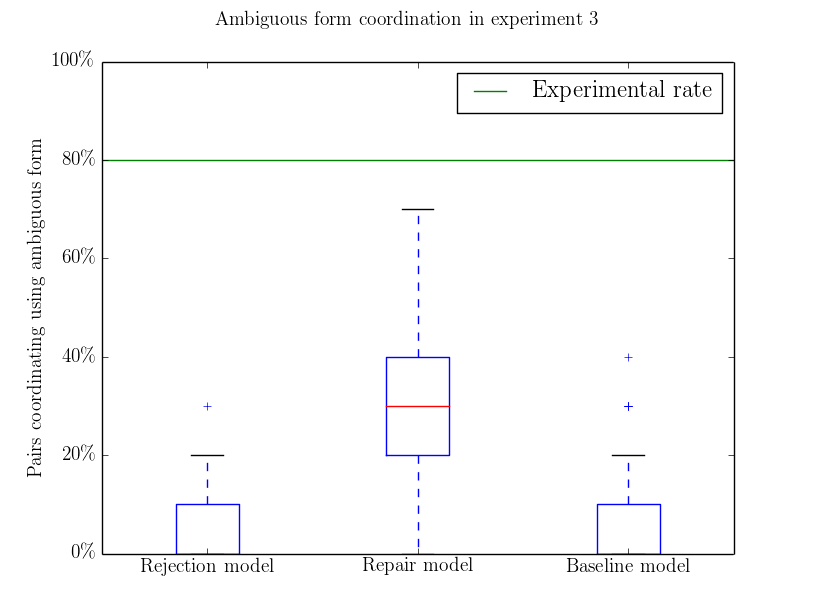
\includegraphics[width=\textwidth]{ambi_coord_exp3.png}
%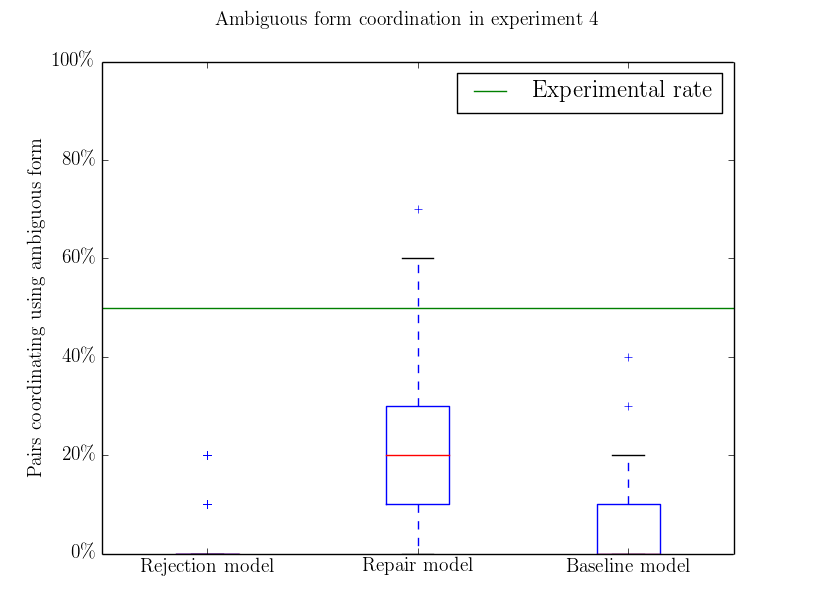
\includegraphics[width=\textwidth]{ambi_coord_exp4.png}
%\end{center}
%
%\begin{center}
%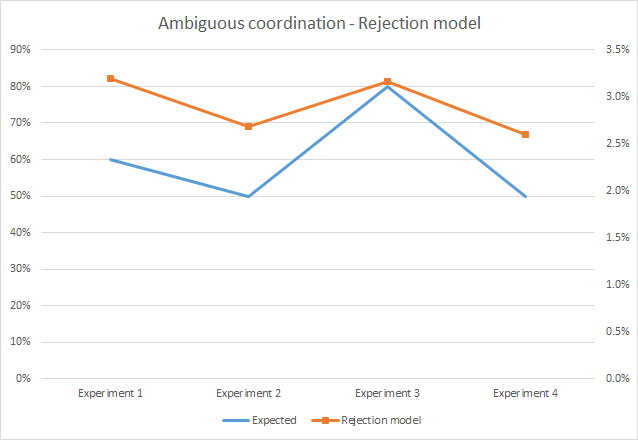
\includegraphics[width=\textwidth]{ambiguous_coordination_rejection.png}
%\textit{Given that these are all at different scales, is there a way to present them together for comparison? How to choose/justify the scaling?}
%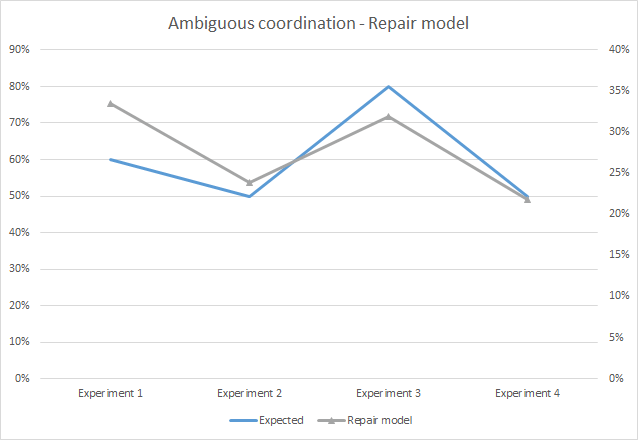
\includegraphics[width=\textwidth]{ambiguous_coordination_repair.png}
%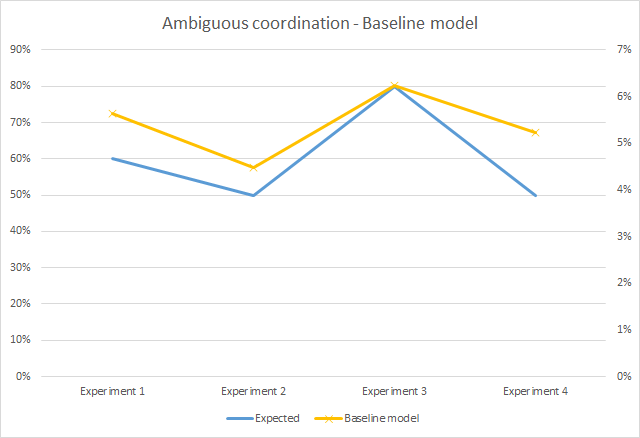
\includegraphics[width=\textwidth]{ambiguous_coordination_baseline.png}
%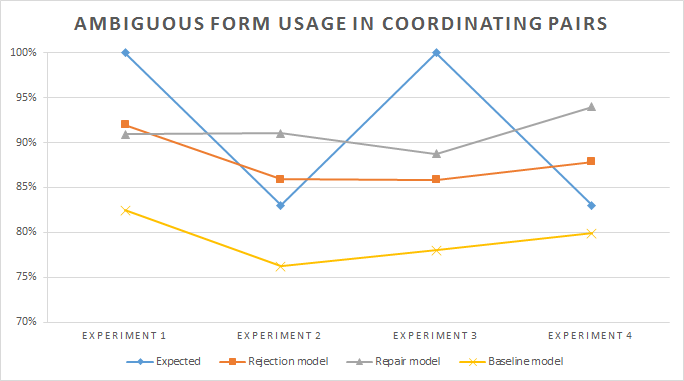
\includegraphics[width=\textwidth]{ambiguous_vs_unambiguous_smaller.png}
%\textit{What is the most appropriate way to measure whether either of the two optimized models tracks the experimental data more effectively than the baseline model?}
%\end{center}

\subsection{Predictions from repair model}
\subsubsection{Cost and reward variation}
As the repair model was shown to outperform both the rejection and baseline models in mimicking experimental data when scaled ($p<0.001$, see \ref{sec:model_comparison}), it was chosen to predict referential coordination behaviours outside those conditions studied in \citeauthor{rohde2012}. The results of varying ambiguous form cost on ambiguous and unambiguous form coordination \textit{ceteris paribus} are presented in Figure \ref{fig:3},\footnote{It should be noted that because coordination rates have been scaled here as per Table \ref{table:3}, the combined rates in some instances exceed $100\%$. The rates could be normalized or the scaling factor adjusted to avoid this; alternatively, an alternative choice of parameters for the model might obviate the need for a scaling factor and, in doing so, eliminate the issue.} while Figure \ref{fig:4} demonstrates the effects of adjusting the number of points awarded for successful communication. As can be seen, the repair model predicts that overall coordination rates (on both ambiguous and unambiguous forms) increase in response to both higher ambiguous form cost and higher successful communication reward.

\begin{figure}
\centering
%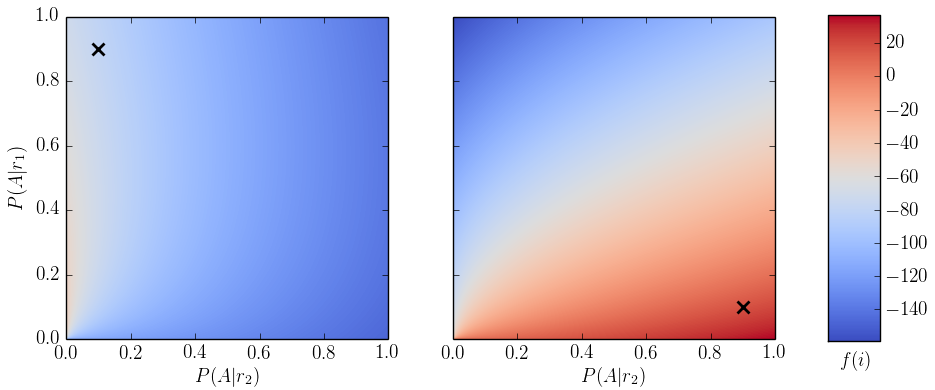
\includegraphics[width=\textwidth]{objective_function_cropped.png}
\scalebox{.65}{%% Creator: Matplotlib, PGF backend
%%
%% To include the figure in your LaTeX document, write
%%   \input{<filename>.pgf}
%%
%% Make sure the required packages are loaded in your preamble
%%   \usepackage{pgf}
%%
%% Figures using additional raster images can only be included by \input if
%% they are in the same directory as the main LaTeX file. For loading figures
%% from other directories you can use the `import` package
%%   \usepackage{import}
%% and then include the figures with
%%   \import{<path to file>}{<filename>.pgf}
%%
%% Matplotlib used the following preamble
%%   \usepackage{fontspec}
%%   \setsansfont{DejaVu Sans}
%%   \setmonofont{DejaVu Sans Mono}
%%
\begingroup%
\makeatletter%
\begin{pgfpicture}%
\pgfpathrectangle{\pgfpointorigin}{\pgfqpoint{6.600000in}{5.300000in}}%
\pgfusepath{use as bounding box, clip}%
\begin{pgfscope}%
\pgfsetbuttcap%
\pgfsetmiterjoin%
\definecolor{currentfill}{rgb}{1.000000,1.000000,1.000000}%
\pgfsetfillcolor{currentfill}%
\pgfsetlinewidth{0.000000pt}%
\definecolor{currentstroke}{rgb}{1.000000,1.000000,1.000000}%
\pgfsetstrokecolor{currentstroke}%
\pgfsetdash{}{0pt}%
\pgfpathmoveto{\pgfqpoint{0.000000in}{0.000000in}}%
\pgfpathlineto{\pgfqpoint{6.600000in}{0.000000in}}%
\pgfpathlineto{\pgfqpoint{6.600000in}{5.300000in}}%
\pgfpathlineto{\pgfqpoint{0.000000in}{5.300000in}}%
\pgfpathclose%
\pgfusepath{fill}%
\end{pgfscope}%
\begin{pgfscope}%
\pgfsetbuttcap%
\pgfsetmiterjoin%
\definecolor{currentfill}{rgb}{1.000000,1.000000,1.000000}%
\pgfsetfillcolor{currentfill}%
\pgfsetlinewidth{0.000000pt}%
\definecolor{currentstroke}{rgb}{0.000000,0.000000,0.000000}%
\pgfsetstrokecolor{currentstroke}%
\pgfsetstrokeopacity{0.000000}%
\pgfsetdash{}{0pt}%
\pgfpathmoveto{\pgfqpoint{0.825000in}{0.530000in}}%
\pgfpathlineto{\pgfqpoint{5.940000in}{0.530000in}}%
\pgfpathlineto{\pgfqpoint{5.940000in}{4.770000in}}%
\pgfpathlineto{\pgfqpoint{0.825000in}{4.770000in}}%
\pgfpathclose%
\pgfusepath{fill}%
\end{pgfscope}%
\begin{pgfscope}%
\pgfpathrectangle{\pgfqpoint{0.825000in}{0.530000in}}{\pgfqpoint{5.115000in}{4.240000in}} %
\pgfusepath{clip}%
\pgfsetrectcap%
\pgfsetroundjoin%
\pgfsetlinewidth{1.003750pt}%
\definecolor{currentstroke}{rgb}{0.000000,0.000000,1.000000}%
\pgfsetstrokecolor{currentstroke}%
\pgfsetdash{}{0pt}%
\pgfpathmoveto{\pgfqpoint{0.825000in}{1.485431in}}%
\pgfpathlineto{\pgfqpoint{1.109167in}{1.615549in}}%
\pgfpathlineto{\pgfqpoint{1.393333in}{1.931547in}}%
\pgfpathlineto{\pgfqpoint{1.677500in}{2.154605in}}%
\pgfpathlineto{\pgfqpoint{1.961667in}{2.281005in}}%
\pgfpathlineto{\pgfqpoint{2.245833in}{2.611874in}}%
\pgfpathlineto{\pgfqpoint{2.530000in}{2.645333in}}%
\pgfpathlineto{\pgfqpoint{2.814167in}{2.920437in}}%
\pgfpathlineto{\pgfqpoint{3.098333in}{3.202977in}}%
\pgfpathlineto{\pgfqpoint{3.382500in}{3.407447in}}%
\pgfpathlineto{\pgfqpoint{3.666667in}{3.515258in}}%
\pgfpathlineto{\pgfqpoint{3.950833in}{3.545000in}}%
\pgfpathlineto{\pgfqpoint{4.235000in}{3.760622in}}%
\pgfpathlineto{\pgfqpoint{4.519167in}{3.864716in}}%
\pgfpathlineto{\pgfqpoint{4.803333in}{3.675117in}}%
\pgfpathlineto{\pgfqpoint{5.087500in}{3.846128in}}%
\pgfpathlineto{\pgfqpoint{5.371667in}{3.760622in}}%
\pgfpathlineto{\pgfqpoint{5.655833in}{3.857281in}}%
\pgfpathlineto{\pgfqpoint{5.940000in}{3.682552in}}%
\pgfusepath{stroke}%
\end{pgfscope}%
\begin{pgfscope}%
\pgfpathrectangle{\pgfqpoint{0.825000in}{0.530000in}}{\pgfqpoint{5.115000in}{4.240000in}} %
\pgfusepath{clip}%
\pgfsetbuttcap%
\pgfsetroundjoin%
\pgfsetlinewidth{1.003750pt}%
\definecolor{currentstroke}{rgb}{0.000000,0.500000,0.000000}%
\pgfsetstrokecolor{currentstroke}%
\pgfsetdash{{6.000000pt}{6.000000pt}}{0.000000pt}%
\pgfpathmoveto{\pgfqpoint{0.825000in}{0.541153in}}%
\pgfpathlineto{\pgfqpoint{1.109167in}{0.544871in}}%
\pgfpathlineto{\pgfqpoint{1.393333in}{0.563459in}}%
\pgfpathlineto{\pgfqpoint{1.677500in}{0.570894in}}%
\pgfpathlineto{\pgfqpoint{1.961667in}{0.600635in}}%
\pgfpathlineto{\pgfqpoint{2.245833in}{0.678705in}}%
\pgfpathlineto{\pgfqpoint{2.530000in}{0.879457in}}%
\pgfpathlineto{\pgfqpoint{2.814167in}{1.113668in}}%
\pgfpathlineto{\pgfqpoint{3.098333in}{1.258656in}}%
\pgfpathlineto{\pgfqpoint{3.382500in}{1.351597in}}%
\pgfpathlineto{\pgfqpoint{3.666667in}{1.422232in}}%
\pgfpathlineto{\pgfqpoint{3.950833in}{1.600678in}}%
\pgfpathlineto{\pgfqpoint{4.235000in}{1.660160in}}%
\pgfpathlineto{\pgfqpoint{4.519167in}{1.630419in}}%
\pgfpathlineto{\pgfqpoint{4.803333in}{1.712207in}}%
\pgfpathlineto{\pgfqpoint{5.087500in}{1.697336in}}%
\pgfpathlineto{\pgfqpoint{5.371667in}{1.808865in}}%
\pgfpathlineto{\pgfqpoint{5.655833in}{1.872065in}}%
\pgfpathlineto{\pgfqpoint{5.940000in}{2.028206in}}%
\pgfusepath{stroke}%
\end{pgfscope}%
\begin{pgfscope}%
\pgfsetrectcap%
\pgfsetmiterjoin%
\pgfsetlinewidth{1.003750pt}%
\definecolor{currentstroke}{rgb}{0.000000,0.000000,0.000000}%
\pgfsetstrokecolor{currentstroke}%
\pgfsetdash{}{0pt}%
\pgfpathmoveto{\pgfqpoint{0.825000in}{4.770000in}}%
\pgfpathlineto{\pgfqpoint{5.940000in}{4.770000in}}%
\pgfusepath{stroke}%
\end{pgfscope}%
\begin{pgfscope}%
\pgfsetrectcap%
\pgfsetmiterjoin%
\pgfsetlinewidth{1.003750pt}%
\definecolor{currentstroke}{rgb}{0.000000,0.000000,0.000000}%
\pgfsetstrokecolor{currentstroke}%
\pgfsetdash{}{0pt}%
\pgfpathmoveto{\pgfqpoint{5.940000in}{0.530000in}}%
\pgfpathlineto{\pgfqpoint{5.940000in}{4.770000in}}%
\pgfusepath{stroke}%
\end{pgfscope}%
\begin{pgfscope}%
\pgfsetrectcap%
\pgfsetmiterjoin%
\pgfsetlinewidth{1.003750pt}%
\definecolor{currentstroke}{rgb}{0.000000,0.000000,0.000000}%
\pgfsetstrokecolor{currentstroke}%
\pgfsetdash{}{0pt}%
\pgfpathmoveto{\pgfqpoint{0.825000in}{0.530000in}}%
\pgfpathlineto{\pgfqpoint{5.940000in}{0.530000in}}%
\pgfusepath{stroke}%
\end{pgfscope}%
\begin{pgfscope}%
\pgfsetrectcap%
\pgfsetmiterjoin%
\pgfsetlinewidth{1.003750pt}%
\definecolor{currentstroke}{rgb}{0.000000,0.000000,0.000000}%
\pgfsetstrokecolor{currentstroke}%
\pgfsetdash{}{0pt}%
\pgfpathmoveto{\pgfqpoint{0.825000in}{0.530000in}}%
\pgfpathlineto{\pgfqpoint{0.825000in}{4.770000in}}%
\pgfusepath{stroke}%
\end{pgfscope}%
\begin{pgfscope}%
\pgfsetbuttcap%
\pgfsetroundjoin%
\definecolor{currentfill}{rgb}{0.000000,0.000000,0.000000}%
\pgfsetfillcolor{currentfill}%
\pgfsetlinewidth{0.501875pt}%
\definecolor{currentstroke}{rgb}{0.000000,0.000000,0.000000}%
\pgfsetstrokecolor{currentstroke}%
\pgfsetdash{}{0pt}%
\pgfsys@defobject{currentmarker}{\pgfqpoint{0.000000in}{0.000000in}}{\pgfqpoint{0.000000in}{0.055556in}}{%
\pgfpathmoveto{\pgfqpoint{0.000000in}{0.000000in}}%
\pgfpathlineto{\pgfqpoint{0.000000in}{0.055556in}}%
\pgfusepath{stroke,fill}%
}%
\begin{pgfscope}%
\pgfsys@transformshift{0.825000in}{0.530000in}%
\pgfsys@useobject{currentmarker}{}%
\end{pgfscope}%
\end{pgfscope}%
\begin{pgfscope}%
\pgfsetbuttcap%
\pgfsetroundjoin%
\definecolor{currentfill}{rgb}{0.000000,0.000000,0.000000}%
\pgfsetfillcolor{currentfill}%
\pgfsetlinewidth{0.501875pt}%
\definecolor{currentstroke}{rgb}{0.000000,0.000000,0.000000}%
\pgfsetstrokecolor{currentstroke}%
\pgfsetdash{}{0pt}%
\pgfsys@defobject{currentmarker}{\pgfqpoint{0.000000in}{-0.055556in}}{\pgfqpoint{0.000000in}{0.000000in}}{%
\pgfpathmoveto{\pgfqpoint{0.000000in}{0.000000in}}%
\pgfpathlineto{\pgfqpoint{0.000000in}{-0.055556in}}%
\pgfusepath{stroke,fill}%
}%
\begin{pgfscope}%
\pgfsys@transformshift{0.825000in}{4.770000in}%
\pgfsys@useobject{currentmarker}{}%
\end{pgfscope}%
\end{pgfscope}%
\begin{pgfscope}%
\pgftext[x=0.825000in,y=0.474444in,,top]{{\sffamily\fontsize{14.000000}{16.800000}\selectfont \(\displaystyle -20\)}}%
\end{pgfscope}%
\begin{pgfscope}%
\pgfsetbuttcap%
\pgfsetroundjoin%
\definecolor{currentfill}{rgb}{0.000000,0.000000,0.000000}%
\pgfsetfillcolor{currentfill}%
\pgfsetlinewidth{0.501875pt}%
\definecolor{currentstroke}{rgb}{0.000000,0.000000,0.000000}%
\pgfsetstrokecolor{currentstroke}%
\pgfsetdash{}{0pt}%
\pgfsys@defobject{currentmarker}{\pgfqpoint{0.000000in}{0.000000in}}{\pgfqpoint{0.000000in}{0.055556in}}{%
\pgfpathmoveto{\pgfqpoint{0.000000in}{0.000000in}}%
\pgfpathlineto{\pgfqpoint{0.000000in}{0.055556in}}%
\pgfusepath{stroke,fill}%
}%
\begin{pgfscope}%
\pgfsys@transformshift{1.393333in}{0.530000in}%
\pgfsys@useobject{currentmarker}{}%
\end{pgfscope}%
\end{pgfscope}%
\begin{pgfscope}%
\pgfsetbuttcap%
\pgfsetroundjoin%
\definecolor{currentfill}{rgb}{0.000000,0.000000,0.000000}%
\pgfsetfillcolor{currentfill}%
\pgfsetlinewidth{0.501875pt}%
\definecolor{currentstroke}{rgb}{0.000000,0.000000,0.000000}%
\pgfsetstrokecolor{currentstroke}%
\pgfsetdash{}{0pt}%
\pgfsys@defobject{currentmarker}{\pgfqpoint{0.000000in}{-0.055556in}}{\pgfqpoint{0.000000in}{0.000000in}}{%
\pgfpathmoveto{\pgfqpoint{0.000000in}{0.000000in}}%
\pgfpathlineto{\pgfqpoint{0.000000in}{-0.055556in}}%
\pgfusepath{stroke,fill}%
}%
\begin{pgfscope}%
\pgfsys@transformshift{1.393333in}{4.770000in}%
\pgfsys@useobject{currentmarker}{}%
\end{pgfscope}%
\end{pgfscope}%
\begin{pgfscope}%
\pgftext[x=1.393333in,y=0.474444in,,top]{{\sffamily\fontsize{14.000000}{16.800000}\selectfont \(\displaystyle 20\)}}%
\end{pgfscope}%
\begin{pgfscope}%
\pgfsetbuttcap%
\pgfsetroundjoin%
\definecolor{currentfill}{rgb}{0.000000,0.000000,0.000000}%
\pgfsetfillcolor{currentfill}%
\pgfsetlinewidth{0.501875pt}%
\definecolor{currentstroke}{rgb}{0.000000,0.000000,0.000000}%
\pgfsetstrokecolor{currentstroke}%
\pgfsetdash{}{0pt}%
\pgfsys@defobject{currentmarker}{\pgfqpoint{0.000000in}{0.000000in}}{\pgfqpoint{0.000000in}{0.055556in}}{%
\pgfpathmoveto{\pgfqpoint{0.000000in}{0.000000in}}%
\pgfpathlineto{\pgfqpoint{0.000000in}{0.055556in}}%
\pgfusepath{stroke,fill}%
}%
\begin{pgfscope}%
\pgfsys@transformshift{1.961667in}{0.530000in}%
\pgfsys@useobject{currentmarker}{}%
\end{pgfscope}%
\end{pgfscope}%
\begin{pgfscope}%
\pgfsetbuttcap%
\pgfsetroundjoin%
\definecolor{currentfill}{rgb}{0.000000,0.000000,0.000000}%
\pgfsetfillcolor{currentfill}%
\pgfsetlinewidth{0.501875pt}%
\definecolor{currentstroke}{rgb}{0.000000,0.000000,0.000000}%
\pgfsetstrokecolor{currentstroke}%
\pgfsetdash{}{0pt}%
\pgfsys@defobject{currentmarker}{\pgfqpoint{0.000000in}{-0.055556in}}{\pgfqpoint{0.000000in}{0.000000in}}{%
\pgfpathmoveto{\pgfqpoint{0.000000in}{0.000000in}}%
\pgfpathlineto{\pgfqpoint{0.000000in}{-0.055556in}}%
\pgfusepath{stroke,fill}%
}%
\begin{pgfscope}%
\pgfsys@transformshift{1.961667in}{4.770000in}%
\pgfsys@useobject{currentmarker}{}%
\end{pgfscope}%
\end{pgfscope}%
\begin{pgfscope}%
\pgftext[x=1.961667in,y=0.474444in,,top]{{\sffamily\fontsize{14.000000}{16.800000}\selectfont \(\displaystyle 60\)}}%
\end{pgfscope}%
\begin{pgfscope}%
\pgfsetbuttcap%
\pgfsetroundjoin%
\definecolor{currentfill}{rgb}{0.000000,0.000000,0.000000}%
\pgfsetfillcolor{currentfill}%
\pgfsetlinewidth{0.501875pt}%
\definecolor{currentstroke}{rgb}{0.000000,0.000000,0.000000}%
\pgfsetstrokecolor{currentstroke}%
\pgfsetdash{}{0pt}%
\pgfsys@defobject{currentmarker}{\pgfqpoint{0.000000in}{0.000000in}}{\pgfqpoint{0.000000in}{0.055556in}}{%
\pgfpathmoveto{\pgfqpoint{0.000000in}{0.000000in}}%
\pgfpathlineto{\pgfqpoint{0.000000in}{0.055556in}}%
\pgfusepath{stroke,fill}%
}%
\begin{pgfscope}%
\pgfsys@transformshift{2.530000in}{0.530000in}%
\pgfsys@useobject{currentmarker}{}%
\end{pgfscope}%
\end{pgfscope}%
\begin{pgfscope}%
\pgfsetbuttcap%
\pgfsetroundjoin%
\definecolor{currentfill}{rgb}{0.000000,0.000000,0.000000}%
\pgfsetfillcolor{currentfill}%
\pgfsetlinewidth{0.501875pt}%
\definecolor{currentstroke}{rgb}{0.000000,0.000000,0.000000}%
\pgfsetstrokecolor{currentstroke}%
\pgfsetdash{}{0pt}%
\pgfsys@defobject{currentmarker}{\pgfqpoint{0.000000in}{-0.055556in}}{\pgfqpoint{0.000000in}{0.000000in}}{%
\pgfpathmoveto{\pgfqpoint{0.000000in}{0.000000in}}%
\pgfpathlineto{\pgfqpoint{0.000000in}{-0.055556in}}%
\pgfusepath{stroke,fill}%
}%
\begin{pgfscope}%
\pgfsys@transformshift{2.530000in}{4.770000in}%
\pgfsys@useobject{currentmarker}{}%
\end{pgfscope}%
\end{pgfscope}%
\begin{pgfscope}%
\pgftext[x=2.530000in,y=0.474444in,,top]{{\sffamily\fontsize{14.000000}{16.800000}\selectfont \(\displaystyle 100\)}}%
\end{pgfscope}%
\begin{pgfscope}%
\pgfsetbuttcap%
\pgfsetroundjoin%
\definecolor{currentfill}{rgb}{0.000000,0.000000,0.000000}%
\pgfsetfillcolor{currentfill}%
\pgfsetlinewidth{0.501875pt}%
\definecolor{currentstroke}{rgb}{0.000000,0.000000,0.000000}%
\pgfsetstrokecolor{currentstroke}%
\pgfsetdash{}{0pt}%
\pgfsys@defobject{currentmarker}{\pgfqpoint{0.000000in}{0.000000in}}{\pgfqpoint{0.000000in}{0.055556in}}{%
\pgfpathmoveto{\pgfqpoint{0.000000in}{0.000000in}}%
\pgfpathlineto{\pgfqpoint{0.000000in}{0.055556in}}%
\pgfusepath{stroke,fill}%
}%
\begin{pgfscope}%
\pgfsys@transformshift{3.098333in}{0.530000in}%
\pgfsys@useobject{currentmarker}{}%
\end{pgfscope}%
\end{pgfscope}%
\begin{pgfscope}%
\pgfsetbuttcap%
\pgfsetroundjoin%
\definecolor{currentfill}{rgb}{0.000000,0.000000,0.000000}%
\pgfsetfillcolor{currentfill}%
\pgfsetlinewidth{0.501875pt}%
\definecolor{currentstroke}{rgb}{0.000000,0.000000,0.000000}%
\pgfsetstrokecolor{currentstroke}%
\pgfsetdash{}{0pt}%
\pgfsys@defobject{currentmarker}{\pgfqpoint{0.000000in}{-0.055556in}}{\pgfqpoint{0.000000in}{0.000000in}}{%
\pgfpathmoveto{\pgfqpoint{0.000000in}{0.000000in}}%
\pgfpathlineto{\pgfqpoint{0.000000in}{-0.055556in}}%
\pgfusepath{stroke,fill}%
}%
\begin{pgfscope}%
\pgfsys@transformshift{3.098333in}{4.770000in}%
\pgfsys@useobject{currentmarker}{}%
\end{pgfscope}%
\end{pgfscope}%
\begin{pgfscope}%
\pgftext[x=3.098333in,y=0.474444in,,top]{{\sffamily\fontsize{14.000000}{16.800000}\selectfont \(\displaystyle 140\)}}%
\end{pgfscope}%
\begin{pgfscope}%
\pgfsetbuttcap%
\pgfsetroundjoin%
\definecolor{currentfill}{rgb}{0.000000,0.000000,0.000000}%
\pgfsetfillcolor{currentfill}%
\pgfsetlinewidth{0.501875pt}%
\definecolor{currentstroke}{rgb}{0.000000,0.000000,0.000000}%
\pgfsetstrokecolor{currentstroke}%
\pgfsetdash{}{0pt}%
\pgfsys@defobject{currentmarker}{\pgfqpoint{0.000000in}{0.000000in}}{\pgfqpoint{0.000000in}{0.055556in}}{%
\pgfpathmoveto{\pgfqpoint{0.000000in}{0.000000in}}%
\pgfpathlineto{\pgfqpoint{0.000000in}{0.055556in}}%
\pgfusepath{stroke,fill}%
}%
\begin{pgfscope}%
\pgfsys@transformshift{3.666667in}{0.530000in}%
\pgfsys@useobject{currentmarker}{}%
\end{pgfscope}%
\end{pgfscope}%
\begin{pgfscope}%
\pgfsetbuttcap%
\pgfsetroundjoin%
\definecolor{currentfill}{rgb}{0.000000,0.000000,0.000000}%
\pgfsetfillcolor{currentfill}%
\pgfsetlinewidth{0.501875pt}%
\definecolor{currentstroke}{rgb}{0.000000,0.000000,0.000000}%
\pgfsetstrokecolor{currentstroke}%
\pgfsetdash{}{0pt}%
\pgfsys@defobject{currentmarker}{\pgfqpoint{0.000000in}{-0.055556in}}{\pgfqpoint{0.000000in}{0.000000in}}{%
\pgfpathmoveto{\pgfqpoint{0.000000in}{0.000000in}}%
\pgfpathlineto{\pgfqpoint{0.000000in}{-0.055556in}}%
\pgfusepath{stroke,fill}%
}%
\begin{pgfscope}%
\pgfsys@transformshift{3.666667in}{4.770000in}%
\pgfsys@useobject{currentmarker}{}%
\end{pgfscope}%
\end{pgfscope}%
\begin{pgfscope}%
\pgftext[x=3.666667in,y=0.474444in,,top]{{\sffamily\fontsize{14.000000}{16.800000}\selectfont \(\displaystyle 180\)}}%
\end{pgfscope}%
\begin{pgfscope}%
\pgfsetbuttcap%
\pgfsetroundjoin%
\definecolor{currentfill}{rgb}{0.000000,0.000000,0.000000}%
\pgfsetfillcolor{currentfill}%
\pgfsetlinewidth{0.501875pt}%
\definecolor{currentstroke}{rgb}{0.000000,0.000000,0.000000}%
\pgfsetstrokecolor{currentstroke}%
\pgfsetdash{}{0pt}%
\pgfsys@defobject{currentmarker}{\pgfqpoint{0.000000in}{0.000000in}}{\pgfqpoint{0.000000in}{0.055556in}}{%
\pgfpathmoveto{\pgfqpoint{0.000000in}{0.000000in}}%
\pgfpathlineto{\pgfqpoint{0.000000in}{0.055556in}}%
\pgfusepath{stroke,fill}%
}%
\begin{pgfscope}%
\pgfsys@transformshift{4.235000in}{0.530000in}%
\pgfsys@useobject{currentmarker}{}%
\end{pgfscope}%
\end{pgfscope}%
\begin{pgfscope}%
\pgfsetbuttcap%
\pgfsetroundjoin%
\definecolor{currentfill}{rgb}{0.000000,0.000000,0.000000}%
\pgfsetfillcolor{currentfill}%
\pgfsetlinewidth{0.501875pt}%
\definecolor{currentstroke}{rgb}{0.000000,0.000000,0.000000}%
\pgfsetstrokecolor{currentstroke}%
\pgfsetdash{}{0pt}%
\pgfsys@defobject{currentmarker}{\pgfqpoint{0.000000in}{-0.055556in}}{\pgfqpoint{0.000000in}{0.000000in}}{%
\pgfpathmoveto{\pgfqpoint{0.000000in}{0.000000in}}%
\pgfpathlineto{\pgfqpoint{0.000000in}{-0.055556in}}%
\pgfusepath{stroke,fill}%
}%
\begin{pgfscope}%
\pgfsys@transformshift{4.235000in}{4.770000in}%
\pgfsys@useobject{currentmarker}{}%
\end{pgfscope}%
\end{pgfscope}%
\begin{pgfscope}%
\pgftext[x=4.235000in,y=0.474444in,,top]{{\sffamily\fontsize{14.000000}{16.800000}\selectfont \(\displaystyle 220\)}}%
\end{pgfscope}%
\begin{pgfscope}%
\pgfsetbuttcap%
\pgfsetroundjoin%
\definecolor{currentfill}{rgb}{0.000000,0.000000,0.000000}%
\pgfsetfillcolor{currentfill}%
\pgfsetlinewidth{0.501875pt}%
\definecolor{currentstroke}{rgb}{0.000000,0.000000,0.000000}%
\pgfsetstrokecolor{currentstroke}%
\pgfsetdash{}{0pt}%
\pgfsys@defobject{currentmarker}{\pgfqpoint{0.000000in}{0.000000in}}{\pgfqpoint{0.000000in}{0.055556in}}{%
\pgfpathmoveto{\pgfqpoint{0.000000in}{0.000000in}}%
\pgfpathlineto{\pgfqpoint{0.000000in}{0.055556in}}%
\pgfusepath{stroke,fill}%
}%
\begin{pgfscope}%
\pgfsys@transformshift{4.803333in}{0.530000in}%
\pgfsys@useobject{currentmarker}{}%
\end{pgfscope}%
\end{pgfscope}%
\begin{pgfscope}%
\pgfsetbuttcap%
\pgfsetroundjoin%
\definecolor{currentfill}{rgb}{0.000000,0.000000,0.000000}%
\pgfsetfillcolor{currentfill}%
\pgfsetlinewidth{0.501875pt}%
\definecolor{currentstroke}{rgb}{0.000000,0.000000,0.000000}%
\pgfsetstrokecolor{currentstroke}%
\pgfsetdash{}{0pt}%
\pgfsys@defobject{currentmarker}{\pgfqpoint{0.000000in}{-0.055556in}}{\pgfqpoint{0.000000in}{0.000000in}}{%
\pgfpathmoveto{\pgfqpoint{0.000000in}{0.000000in}}%
\pgfpathlineto{\pgfqpoint{0.000000in}{-0.055556in}}%
\pgfusepath{stroke,fill}%
}%
\begin{pgfscope}%
\pgfsys@transformshift{4.803333in}{4.770000in}%
\pgfsys@useobject{currentmarker}{}%
\end{pgfscope}%
\end{pgfscope}%
\begin{pgfscope}%
\pgftext[x=4.803333in,y=0.474444in,,top]{{\sffamily\fontsize{14.000000}{16.800000}\selectfont \(\displaystyle 260\)}}%
\end{pgfscope}%
\begin{pgfscope}%
\pgfsetbuttcap%
\pgfsetroundjoin%
\definecolor{currentfill}{rgb}{0.000000,0.000000,0.000000}%
\pgfsetfillcolor{currentfill}%
\pgfsetlinewidth{0.501875pt}%
\definecolor{currentstroke}{rgb}{0.000000,0.000000,0.000000}%
\pgfsetstrokecolor{currentstroke}%
\pgfsetdash{}{0pt}%
\pgfsys@defobject{currentmarker}{\pgfqpoint{0.000000in}{0.000000in}}{\pgfqpoint{0.000000in}{0.055556in}}{%
\pgfpathmoveto{\pgfqpoint{0.000000in}{0.000000in}}%
\pgfpathlineto{\pgfqpoint{0.000000in}{0.055556in}}%
\pgfusepath{stroke,fill}%
}%
\begin{pgfscope}%
\pgfsys@transformshift{5.371667in}{0.530000in}%
\pgfsys@useobject{currentmarker}{}%
\end{pgfscope}%
\end{pgfscope}%
\begin{pgfscope}%
\pgfsetbuttcap%
\pgfsetroundjoin%
\definecolor{currentfill}{rgb}{0.000000,0.000000,0.000000}%
\pgfsetfillcolor{currentfill}%
\pgfsetlinewidth{0.501875pt}%
\definecolor{currentstroke}{rgb}{0.000000,0.000000,0.000000}%
\pgfsetstrokecolor{currentstroke}%
\pgfsetdash{}{0pt}%
\pgfsys@defobject{currentmarker}{\pgfqpoint{0.000000in}{-0.055556in}}{\pgfqpoint{0.000000in}{0.000000in}}{%
\pgfpathmoveto{\pgfqpoint{0.000000in}{0.000000in}}%
\pgfpathlineto{\pgfqpoint{0.000000in}{-0.055556in}}%
\pgfusepath{stroke,fill}%
}%
\begin{pgfscope}%
\pgfsys@transformshift{5.371667in}{4.770000in}%
\pgfsys@useobject{currentmarker}{}%
\end{pgfscope}%
\end{pgfscope}%
\begin{pgfscope}%
\pgftext[x=5.371667in,y=0.474444in,,top]{{\sffamily\fontsize{14.000000}{16.800000}\selectfont \(\displaystyle 300\)}}%
\end{pgfscope}%
\begin{pgfscope}%
\pgfsetbuttcap%
\pgfsetroundjoin%
\definecolor{currentfill}{rgb}{0.000000,0.000000,0.000000}%
\pgfsetfillcolor{currentfill}%
\pgfsetlinewidth{0.501875pt}%
\definecolor{currentstroke}{rgb}{0.000000,0.000000,0.000000}%
\pgfsetstrokecolor{currentstroke}%
\pgfsetdash{}{0pt}%
\pgfsys@defobject{currentmarker}{\pgfqpoint{0.000000in}{0.000000in}}{\pgfqpoint{0.000000in}{0.055556in}}{%
\pgfpathmoveto{\pgfqpoint{0.000000in}{0.000000in}}%
\pgfpathlineto{\pgfqpoint{0.000000in}{0.055556in}}%
\pgfusepath{stroke,fill}%
}%
\begin{pgfscope}%
\pgfsys@transformshift{5.940000in}{0.530000in}%
\pgfsys@useobject{currentmarker}{}%
\end{pgfscope}%
\end{pgfscope}%
\begin{pgfscope}%
\pgfsetbuttcap%
\pgfsetroundjoin%
\definecolor{currentfill}{rgb}{0.000000,0.000000,0.000000}%
\pgfsetfillcolor{currentfill}%
\pgfsetlinewidth{0.501875pt}%
\definecolor{currentstroke}{rgb}{0.000000,0.000000,0.000000}%
\pgfsetstrokecolor{currentstroke}%
\pgfsetdash{}{0pt}%
\pgfsys@defobject{currentmarker}{\pgfqpoint{0.000000in}{-0.055556in}}{\pgfqpoint{0.000000in}{0.000000in}}{%
\pgfpathmoveto{\pgfqpoint{0.000000in}{0.000000in}}%
\pgfpathlineto{\pgfqpoint{0.000000in}{-0.055556in}}%
\pgfusepath{stroke,fill}%
}%
\begin{pgfscope}%
\pgfsys@transformshift{5.940000in}{4.770000in}%
\pgfsys@useobject{currentmarker}{}%
\end{pgfscope}%
\end{pgfscope}%
\begin{pgfscope}%
\pgftext[x=5.940000in,y=0.474444in,,top]{{\sffamily\fontsize{14.000000}{16.800000}\selectfont \(\displaystyle 340\)}}%
\end{pgfscope}%
\begin{pgfscope}%
\pgftext[x=3.382500in,y=0.216822in,,top]{{\sffamily\fontsize{18.000000}{18.800000}\selectfont \(\displaystyle cost_A\)}}%
\end{pgfscope}%
\begin{pgfscope}%
\pgfsetbuttcap%
\pgfsetroundjoin%
\definecolor{currentfill}{rgb}{0.000000,0.000000,0.000000}%
\pgfsetfillcolor{currentfill}%
\pgfsetlinewidth{0.501875pt}%
\definecolor{currentstroke}{rgb}{0.000000,0.000000,0.000000}%
\pgfsetstrokecolor{currentstroke}%
\pgfsetdash{}{0pt}%
\pgfsys@defobject{currentmarker}{\pgfqpoint{0.000000in}{0.000000in}}{\pgfqpoint{0.055556in}{0.000000in}}{%
\pgfpathmoveto{\pgfqpoint{0.000000in}{0.000000in}}%
\pgfpathlineto{\pgfqpoint{0.055556in}{0.000000in}}%
\pgfusepath{stroke,fill}%
}%
\begin{pgfscope}%
\pgfsys@transformshift{0.825000in}{0.530000in}%
\pgfsys@useobject{currentmarker}{}%
\end{pgfscope}%
\end{pgfscope}%
\begin{pgfscope}%
\pgfsetbuttcap%
\pgfsetroundjoin%
\definecolor{currentfill}{rgb}{0.000000,0.000000,0.000000}%
\pgfsetfillcolor{currentfill}%
\pgfsetlinewidth{0.501875pt}%
\definecolor{currentstroke}{rgb}{0.000000,0.000000,0.000000}%
\pgfsetstrokecolor{currentstroke}%
\pgfsetdash{}{0pt}%
\pgfsys@defobject{currentmarker}{\pgfqpoint{-0.055556in}{0.000000in}}{\pgfqpoint{0.000000in}{0.000000in}}{%
\pgfpathmoveto{\pgfqpoint{0.000000in}{0.000000in}}%
\pgfpathlineto{\pgfqpoint{-0.055556in}{0.000000in}}%
\pgfusepath{stroke,fill}%
}%
\begin{pgfscope}%
\pgfsys@transformshift{5.940000in}{0.530000in}%
\pgfsys@useobject{currentmarker}{}%
\end{pgfscope}%
\end{pgfscope}%
\begin{pgfscope}%
\pgftext[x=0.769444in,y=0.530000in,right,]{{\sffamily\fontsize{14.000000}{16.800000}\selectfont \(\displaystyle 0\%\)}}%
\end{pgfscope}%
\begin{pgfscope}%
\pgfsetbuttcap%
\pgfsetroundjoin%
\definecolor{currentfill}{rgb}{0.000000,0.000000,0.000000}%
\pgfsetfillcolor{currentfill}%
\pgfsetlinewidth{0.501875pt}%
\definecolor{currentstroke}{rgb}{0.000000,0.000000,0.000000}%
\pgfsetstrokecolor{currentstroke}%
\pgfsetdash{}{0pt}%
\pgfsys@defobject{currentmarker}{\pgfqpoint{0.000000in}{0.000000in}}{\pgfqpoint{0.055556in}{0.000000in}}{%
\pgfpathmoveto{\pgfqpoint{0.000000in}{0.000000in}}%
\pgfpathlineto{\pgfqpoint{0.055556in}{0.000000in}}%
\pgfusepath{stroke,fill}%
}%
\begin{pgfscope}%
\pgfsys@transformshift{0.825000in}{1.378000in}%
\pgfsys@useobject{currentmarker}{}%
\end{pgfscope}%
\end{pgfscope}%
\begin{pgfscope}%
\pgfsetbuttcap%
\pgfsetroundjoin%
\definecolor{currentfill}{rgb}{0.000000,0.000000,0.000000}%
\pgfsetfillcolor{currentfill}%
\pgfsetlinewidth{0.501875pt}%
\definecolor{currentstroke}{rgb}{0.000000,0.000000,0.000000}%
\pgfsetstrokecolor{currentstroke}%
\pgfsetdash{}{0pt}%
\pgfsys@defobject{currentmarker}{\pgfqpoint{-0.055556in}{0.000000in}}{\pgfqpoint{0.000000in}{0.000000in}}{%
\pgfpathmoveto{\pgfqpoint{0.000000in}{0.000000in}}%
\pgfpathlineto{\pgfqpoint{-0.055556in}{0.000000in}}%
\pgfusepath{stroke,fill}%
}%
\begin{pgfscope}%
\pgfsys@transformshift{5.940000in}{1.378000in}%
\pgfsys@useobject{currentmarker}{}%
\end{pgfscope}%
\end{pgfscope}%
\begin{pgfscope}%
\pgftext[x=0.769444in,y=1.378000in,right,]{{\sffamily\fontsize{14.000000}{16.800000}\selectfont \(\displaystyle 20\%\)}}%
\end{pgfscope}%
\begin{pgfscope}%
\pgfsetbuttcap%
\pgfsetroundjoin%
\definecolor{currentfill}{rgb}{0.000000,0.000000,0.000000}%
\pgfsetfillcolor{currentfill}%
\pgfsetlinewidth{0.501875pt}%
\definecolor{currentstroke}{rgb}{0.000000,0.000000,0.000000}%
\pgfsetstrokecolor{currentstroke}%
\pgfsetdash{}{0pt}%
\pgfsys@defobject{currentmarker}{\pgfqpoint{0.000000in}{0.000000in}}{\pgfqpoint{0.055556in}{0.000000in}}{%
\pgfpathmoveto{\pgfqpoint{0.000000in}{0.000000in}}%
\pgfpathlineto{\pgfqpoint{0.055556in}{0.000000in}}%
\pgfusepath{stroke,fill}%
}%
\begin{pgfscope}%
\pgfsys@transformshift{0.825000in}{2.226000in}%
\pgfsys@useobject{currentmarker}{}%
\end{pgfscope}%
\end{pgfscope}%
\begin{pgfscope}%
\pgfsetbuttcap%
\pgfsetroundjoin%
\definecolor{currentfill}{rgb}{0.000000,0.000000,0.000000}%
\pgfsetfillcolor{currentfill}%
\pgfsetlinewidth{0.501875pt}%
\definecolor{currentstroke}{rgb}{0.000000,0.000000,0.000000}%
\pgfsetstrokecolor{currentstroke}%
\pgfsetdash{}{0pt}%
\pgfsys@defobject{currentmarker}{\pgfqpoint{-0.055556in}{0.000000in}}{\pgfqpoint{0.000000in}{0.000000in}}{%
\pgfpathmoveto{\pgfqpoint{0.000000in}{0.000000in}}%
\pgfpathlineto{\pgfqpoint{-0.055556in}{0.000000in}}%
\pgfusepath{stroke,fill}%
}%
\begin{pgfscope}%
\pgfsys@transformshift{5.940000in}{2.226000in}%
\pgfsys@useobject{currentmarker}{}%
\end{pgfscope}%
\end{pgfscope}%
\begin{pgfscope}%
\pgftext[x=0.769444in,y=2.226000in,right,]{{\sffamily\fontsize{14.000000}{16.800000}\selectfont \(\displaystyle 40\%\)}}%
\end{pgfscope}%
\begin{pgfscope}%
\pgfsetbuttcap%
\pgfsetroundjoin%
\definecolor{currentfill}{rgb}{0.000000,0.000000,0.000000}%
\pgfsetfillcolor{currentfill}%
\pgfsetlinewidth{0.501875pt}%
\definecolor{currentstroke}{rgb}{0.000000,0.000000,0.000000}%
\pgfsetstrokecolor{currentstroke}%
\pgfsetdash{}{0pt}%
\pgfsys@defobject{currentmarker}{\pgfqpoint{0.000000in}{0.000000in}}{\pgfqpoint{0.055556in}{0.000000in}}{%
\pgfpathmoveto{\pgfqpoint{0.000000in}{0.000000in}}%
\pgfpathlineto{\pgfqpoint{0.055556in}{0.000000in}}%
\pgfusepath{stroke,fill}%
}%
\begin{pgfscope}%
\pgfsys@transformshift{0.825000in}{3.074000in}%
\pgfsys@useobject{currentmarker}{}%
\end{pgfscope}%
\end{pgfscope}%
\begin{pgfscope}%
\pgfsetbuttcap%
\pgfsetroundjoin%
\definecolor{currentfill}{rgb}{0.000000,0.000000,0.000000}%
\pgfsetfillcolor{currentfill}%
\pgfsetlinewidth{0.501875pt}%
\definecolor{currentstroke}{rgb}{0.000000,0.000000,0.000000}%
\pgfsetstrokecolor{currentstroke}%
\pgfsetdash{}{0pt}%
\pgfsys@defobject{currentmarker}{\pgfqpoint{-0.055556in}{0.000000in}}{\pgfqpoint{0.000000in}{0.000000in}}{%
\pgfpathmoveto{\pgfqpoint{0.000000in}{0.000000in}}%
\pgfpathlineto{\pgfqpoint{-0.055556in}{0.000000in}}%
\pgfusepath{stroke,fill}%
}%
\begin{pgfscope}%
\pgfsys@transformshift{5.940000in}{3.074000in}%
\pgfsys@useobject{currentmarker}{}%
\end{pgfscope}%
\end{pgfscope}%
\begin{pgfscope}%
\pgftext[x=0.769444in,y=3.074000in,right,]{{\sffamily\fontsize{14.000000}{16.800000}\selectfont \(\displaystyle 60\%\)}}%
\end{pgfscope}%
\begin{pgfscope}%
\pgfsetbuttcap%
\pgfsetroundjoin%
\definecolor{currentfill}{rgb}{0.000000,0.000000,0.000000}%
\pgfsetfillcolor{currentfill}%
\pgfsetlinewidth{0.501875pt}%
\definecolor{currentstroke}{rgb}{0.000000,0.000000,0.000000}%
\pgfsetstrokecolor{currentstroke}%
\pgfsetdash{}{0pt}%
\pgfsys@defobject{currentmarker}{\pgfqpoint{0.000000in}{0.000000in}}{\pgfqpoint{0.055556in}{0.000000in}}{%
\pgfpathmoveto{\pgfqpoint{0.000000in}{0.000000in}}%
\pgfpathlineto{\pgfqpoint{0.055556in}{0.000000in}}%
\pgfusepath{stroke,fill}%
}%
\begin{pgfscope}%
\pgfsys@transformshift{0.825000in}{3.922000in}%
\pgfsys@useobject{currentmarker}{}%
\end{pgfscope}%
\end{pgfscope}%
\begin{pgfscope}%
\pgfsetbuttcap%
\pgfsetroundjoin%
\definecolor{currentfill}{rgb}{0.000000,0.000000,0.000000}%
\pgfsetfillcolor{currentfill}%
\pgfsetlinewidth{0.501875pt}%
\definecolor{currentstroke}{rgb}{0.000000,0.000000,0.000000}%
\pgfsetstrokecolor{currentstroke}%
\pgfsetdash{}{0pt}%
\pgfsys@defobject{currentmarker}{\pgfqpoint{-0.055556in}{0.000000in}}{\pgfqpoint{0.000000in}{0.000000in}}{%
\pgfpathmoveto{\pgfqpoint{0.000000in}{0.000000in}}%
\pgfpathlineto{\pgfqpoint{-0.055556in}{0.000000in}}%
\pgfusepath{stroke,fill}%
}%
\begin{pgfscope}%
\pgfsys@transformshift{5.940000in}{3.922000in}%
\pgfsys@useobject{currentmarker}{}%
\end{pgfscope}%
\end{pgfscope}%
\begin{pgfscope}%
\pgftext[x=0.769444in,y=3.922000in,right,]{{\sffamily\fontsize{14.000000}{16.800000}\selectfont \(\displaystyle 80\%\)}}%
\end{pgfscope}%
\begin{pgfscope}%
\pgfsetbuttcap%
\pgfsetroundjoin%
\definecolor{currentfill}{rgb}{0.000000,0.000000,0.000000}%
\pgfsetfillcolor{currentfill}%
\pgfsetlinewidth{0.501875pt}%
\definecolor{currentstroke}{rgb}{0.000000,0.000000,0.000000}%
\pgfsetstrokecolor{currentstroke}%
\pgfsetdash{}{0pt}%
\pgfsys@defobject{currentmarker}{\pgfqpoint{0.000000in}{0.000000in}}{\pgfqpoint{0.055556in}{0.000000in}}{%
\pgfpathmoveto{\pgfqpoint{0.000000in}{0.000000in}}%
\pgfpathlineto{\pgfqpoint{0.055556in}{0.000000in}}%
\pgfusepath{stroke,fill}%
}%
\begin{pgfscope}%
\pgfsys@transformshift{0.825000in}{4.770000in}%
\pgfsys@useobject{currentmarker}{}%
\end{pgfscope}%
\end{pgfscope}%
\begin{pgfscope}%
\pgfsetbuttcap%
\pgfsetroundjoin%
\definecolor{currentfill}{rgb}{0.000000,0.000000,0.000000}%
\pgfsetfillcolor{currentfill}%
\pgfsetlinewidth{0.501875pt}%
\definecolor{currentstroke}{rgb}{0.000000,0.000000,0.000000}%
\pgfsetstrokecolor{currentstroke}%
\pgfsetdash{}{0pt}%
\pgfsys@defobject{currentmarker}{\pgfqpoint{-0.055556in}{0.000000in}}{\pgfqpoint{0.000000in}{0.000000in}}{%
\pgfpathmoveto{\pgfqpoint{0.000000in}{0.000000in}}%
\pgfpathlineto{\pgfqpoint{-0.055556in}{0.000000in}}%
\pgfusepath{stroke,fill}%
}%
\begin{pgfscope}%
\pgfsys@transformshift{5.940000in}{4.770000in}%
\pgfsys@useobject{currentmarker}{}%
\end{pgfscope}%
\end{pgfscope}%
\begin{pgfscope}%
\pgftext[x=0.769444in,y=4.770000in,right,]{{\sffamily\fontsize{14.000000}{16.800000}\selectfont \(\displaystyle 100\%\)}}%
\end{pgfscope}%
\begin{pgfscope}%
\pgftext[x=0.247587in,y=2.650000in,,bottom,rotate=90.000000]{{\sffamily\fontsize{18.000000}{18.800000}\selectfont \textrm{Coordination rate}}}%
\end{pgfscope}%
\begin{pgfscope}%
\pgfsetbuttcap%
\pgfsetmiterjoin%
\definecolor{currentfill}{rgb}{1.000000,1.000000,1.000000}%
\pgfsetfillcolor{currentfill}%
\pgfsetlinewidth{1.003750pt}%
\definecolor{currentstroke}{rgb}{0.000000,0.000000,0.000000}%
\pgfsetstrokecolor{currentstroke}%
\pgfsetdash{}{0pt}%
\pgfpathmoveto{\pgfqpoint{0.922222in}{4.072389in}}%
\pgfpathlineto{\pgfqpoint{3.198609in}{4.072389in}}%
\pgfpathlineto{\pgfqpoint{3.198609in}{4.672778in}}%
\pgfpathlineto{\pgfqpoint{0.922222in}{4.672778in}}%
\pgfpathclose%
\pgfusepath{stroke,fill}%
\end{pgfscope}%
\begin{pgfscope}%
\pgfsetrectcap%
\pgfsetroundjoin%
\pgfsetlinewidth{1.003750pt}%
\definecolor{currentstroke}{rgb}{0.000000,0.000000,1.000000}%
\pgfsetstrokecolor{currentstroke}%
\pgfsetdash{}{0pt}%
\pgfpathmoveto{\pgfqpoint{1.058333in}{4.526944in}}%
\pgfpathlineto{\pgfqpoint{1.330556in}{4.526944in}}%
\pgfusepath{stroke}%
\end{pgfscope}%
\begin{pgfscope}%
\pgftext[x=1.544444in,y=4.458889in,left,base]{{\rmfamily\fontsize{14.000000}{16.800000}\selectfont Ambiguous form}}%
\end{pgfscope}%
\begin{pgfscope}%
\pgfsetbuttcap%
\pgfsetroundjoin%
\pgfsetlinewidth{1.003750pt}%
\definecolor{currentstroke}{rgb}{0.000000,0.500000,0.000000}%
\pgfsetstrokecolor{currentstroke}%
\pgfsetdash{{6.000000pt}{6.000000pt}}{0.000000pt}%
\pgfpathmoveto{\pgfqpoint{1.058333in}{4.255889in}}%
\pgfpathlineto{\pgfqpoint{1.330556in}{4.255889in}}%
\pgfusepath{stroke}%
\end{pgfscope}%
\begin{pgfscope}%
\pgftext[x=1.544444in,y=4.187833in,left,base]{{\rmfamily\fontsize{14.000000}{16.800000}\selectfont Unambiguous form}}%
\end{pgfscope}%
\end{pgfpicture}%
\makeatother%
\endgroup%
}
\caption{Average entrainment rates in Experiment 1 with ambiguous form cost varied, as predicted by the repair model.}
\label{fig:3}
\end{figure}

\begin{figure}
\centering
%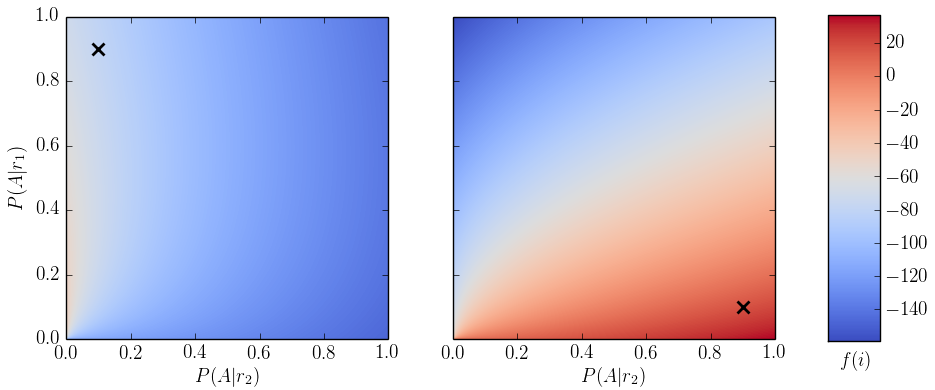
\includegraphics[width=\textwidth]{objective_function_cropped.png}
\scalebox{.65}{%% Creator: Matplotlib, PGF backend
%%
%% To include the figure in your LaTeX document, write
%%   \input{<filename>.pgf}
%%
%% Make sure the required packages are loaded in your preamble
%%   \usepackage{pgf}
%%
%% Figures using additional raster images can only be included by \input if
%% they are in the same directory as the main LaTeX file. For loading figures
%% from other directories you can use the `import` package
%%   \usepackage{import}
%% and then include the figures with
%%   \import{<path to file>}{<filename>.pgf}
%%
%% Matplotlib used the following preamble
%%   \usepackage{fontspec}
%%   \setsansfont{DejaVu Sans}
%%   \setmonofont{DejaVu Sans Mono}
%%
\begingroup%
\makeatletter%
\begin{pgfpicture}%
\pgfpathrectangle{\pgfpointorigin}{\pgfqpoint{6.687500in}{5.325000in}}%
\pgfusepath{use as bounding box, clip}%
\begin{pgfscope}%
\pgfsetbuttcap%
\pgfsetmiterjoin%
\definecolor{currentfill}{rgb}{1.000000,1.000000,1.000000}%
\pgfsetfillcolor{currentfill}%
\pgfsetlinewidth{0.000000pt}%
\definecolor{currentstroke}{rgb}{1.000000,1.000000,1.000000}%
\pgfsetstrokecolor{currentstroke}%
\pgfsetdash{}{0pt}%
\pgfpathmoveto{\pgfqpoint{0.000000in}{0.000000in}}%
\pgfpathlineto{\pgfqpoint{6.687500in}{0.000000in}}%
\pgfpathlineto{\pgfqpoint{6.687500in}{5.325000in}}%
\pgfpathlineto{\pgfqpoint{0.000000in}{5.325000in}}%
\pgfpathclose%
\pgfusepath{fill}%
\end{pgfscope}%
\begin{pgfscope}%
\pgfsetbuttcap%
\pgfsetmiterjoin%
\definecolor{currentfill}{rgb}{1.000000,1.000000,1.000000}%
\pgfsetfillcolor{currentfill}%
\pgfsetlinewidth{0.000000pt}%
\definecolor{currentstroke}{rgb}{0.000000,0.000000,0.000000}%
\pgfsetstrokecolor{currentstroke}%
\pgfsetstrokeopacity{0.000000}%
\pgfsetdash{}{0pt}%
\pgfpathmoveto{\pgfqpoint{0.835938in}{0.532500in}}%
\pgfpathlineto{\pgfqpoint{6.018750in}{0.532500in}}%
\pgfpathlineto{\pgfqpoint{6.018750in}{4.792500in}}%
\pgfpathlineto{\pgfqpoint{0.835938in}{4.792500in}}%
\pgfpathclose%
\pgfusepath{fill}%
\end{pgfscope}%
\begin{pgfscope}%
\pgfpathrectangle{\pgfqpoint{0.835938in}{0.532500in}}{\pgfqpoint{5.182812in}{4.260000in}} %
\pgfusepath{clip}%
\pgfsetrectcap%
\pgfsetroundjoin%
\pgfsetlinewidth{1.003750pt}%
\definecolor{currentstroke}{rgb}{0.000000,0.000000,1.000000}%
\pgfsetstrokecolor{currentstroke}%
\pgfsetdash{}{0pt}%
\pgfpathmoveto{\pgfqpoint{0.835938in}{1.249652in}}%
\pgfpathlineto{\pgfqpoint{1.123872in}{1.492438in}}%
\pgfpathlineto{\pgfqpoint{1.411806in}{1.727754in}}%
\pgfpathlineto{\pgfqpoint{1.699740in}{2.108741in}}%
\pgfpathlineto{\pgfqpoint{1.987674in}{2.175974in}}%
\pgfpathlineto{\pgfqpoint{2.275608in}{2.463582in}}%
\pgfpathlineto{\pgfqpoint{2.563542in}{2.631664in}}%
\pgfpathlineto{\pgfqpoint{2.851476in}{3.128442in}}%
\pgfpathlineto{\pgfqpoint{3.139410in}{3.427255in}}%
\pgfpathlineto{\pgfqpoint{3.427344in}{3.546781in}}%
\pgfpathlineto{\pgfqpoint{3.715278in}{3.729804in}}%
\pgfpathlineto{\pgfqpoint{4.003212in}{3.718598in}}%
\pgfpathlineto{\pgfqpoint{4.291146in}{3.815713in}}%
\pgfpathlineto{\pgfqpoint{4.579080in}{3.886681in}}%
\pgfpathlineto{\pgfqpoint{4.867014in}{4.103321in}}%
\pgfpathlineto{\pgfqpoint{5.154948in}{3.968855in}}%
\pgfpathlineto{\pgfqpoint{5.442882in}{4.058499in}}%
\pgfpathlineto{\pgfqpoint{5.730816in}{4.047293in}}%
\pgfpathlineto{\pgfqpoint{6.018750in}{4.166818in}}%
\pgfusepath{stroke}%
\end{pgfscope}%
\begin{pgfscope}%
\pgfpathrectangle{\pgfqpoint{0.835938in}{0.532500in}}{\pgfqpoint{5.182812in}{4.260000in}} %
\pgfusepath{clip}%
\pgfsetbuttcap%
\pgfsetroundjoin%
\pgfsetlinewidth{1.003750pt}%
\definecolor{currentstroke}{rgb}{0.000000,0.500000,0.000000}%
\pgfsetstrokecolor{currentstroke}%
\pgfsetdash{{6.000000pt}{6.000000pt}}{0.000000pt}%
\pgfpathmoveto{\pgfqpoint{0.835938in}{0.562381in}}%
\pgfpathlineto{\pgfqpoint{1.123872in}{0.547441in}}%
\pgfpathlineto{\pgfqpoint{1.411806in}{0.554911in}}%
\pgfpathlineto{\pgfqpoint{1.699740in}{0.588528in}}%
\pgfpathlineto{\pgfqpoint{1.987674in}{0.633350in}}%
\pgfpathlineto{\pgfqpoint{2.275608in}{0.681907in}}%
\pgfpathlineto{\pgfqpoint{2.563542in}{0.756610in}}%
\pgfpathlineto{\pgfqpoint{2.851476in}{0.891076in}}%
\pgfpathlineto{\pgfqpoint{3.139410in}{0.917222in}}%
\pgfpathlineto{\pgfqpoint{3.427344in}{1.044218in}}%
\pgfpathlineto{\pgfqpoint{3.715278in}{1.182419in}}%
\pgfpathlineto{\pgfqpoint{4.003212in}{1.204830in}}%
\pgfpathlineto{\pgfqpoint{4.291146in}{1.216036in}}%
\pgfpathlineto{\pgfqpoint{4.579080in}{1.230976in}}%
\pgfpathlineto{\pgfqpoint{4.867014in}{1.287004in}}%
\pgfpathlineto{\pgfqpoint{5.154948in}{1.372913in}}%
\pgfpathlineto{\pgfqpoint{5.442882in}{1.275798in}}%
\pgfpathlineto{\pgfqpoint{5.730816in}{1.402794in}}%
\pgfpathlineto{\pgfqpoint{6.018750in}{1.384118in}}%
\pgfusepath{stroke}%
\end{pgfscope}%
\begin{pgfscope}%
\pgfsetrectcap%
\pgfsetmiterjoin%
\pgfsetlinewidth{1.003750pt}%
\definecolor{currentstroke}{rgb}{0.000000,0.000000,0.000000}%
\pgfsetstrokecolor{currentstroke}%
\pgfsetdash{}{0pt}%
\pgfpathmoveto{\pgfqpoint{0.835938in}{4.792500in}}%
\pgfpathlineto{\pgfqpoint{6.018750in}{4.792500in}}%
\pgfusepath{stroke}%
\end{pgfscope}%
\begin{pgfscope}%
\pgfsetrectcap%
\pgfsetmiterjoin%
\pgfsetlinewidth{1.003750pt}%
\definecolor{currentstroke}{rgb}{0.000000,0.000000,0.000000}%
\pgfsetstrokecolor{currentstroke}%
\pgfsetdash{}{0pt}%
\pgfpathmoveto{\pgfqpoint{6.018750in}{0.532500in}}%
\pgfpathlineto{\pgfqpoint{6.018750in}{4.792500in}}%
\pgfusepath{stroke}%
\end{pgfscope}%
\begin{pgfscope}%
\pgfsetrectcap%
\pgfsetmiterjoin%
\pgfsetlinewidth{1.003750pt}%
\definecolor{currentstroke}{rgb}{0.000000,0.000000,0.000000}%
\pgfsetstrokecolor{currentstroke}%
\pgfsetdash{}{0pt}%
\pgfpathmoveto{\pgfqpoint{0.835938in}{0.532500in}}%
\pgfpathlineto{\pgfqpoint{6.018750in}{0.532500in}}%
\pgfusepath{stroke}%
\end{pgfscope}%
\begin{pgfscope}%
\pgfsetrectcap%
\pgfsetmiterjoin%
\pgfsetlinewidth{1.003750pt}%
\definecolor{currentstroke}{rgb}{0.000000,0.000000,0.000000}%
\pgfsetstrokecolor{currentstroke}%
\pgfsetdash{}{0pt}%
\pgfpathmoveto{\pgfqpoint{0.835938in}{0.532500in}}%
\pgfpathlineto{\pgfqpoint{0.835938in}{4.792500in}}%
\pgfusepath{stroke}%
\end{pgfscope}%
\begin{pgfscope}%
\pgfsetbuttcap%
\pgfsetroundjoin%
\definecolor{currentfill}{rgb}{0.000000,0.000000,0.000000}%
\pgfsetfillcolor{currentfill}%
\pgfsetlinewidth{0.501875pt}%
\definecolor{currentstroke}{rgb}{0.000000,0.000000,0.000000}%
\pgfsetstrokecolor{currentstroke}%
\pgfsetdash{}{0pt}%
\pgfsys@defobject{currentmarker}{\pgfqpoint{0.000000in}{0.000000in}}{\pgfqpoint{0.000000in}{0.055556in}}{%
\pgfpathmoveto{\pgfqpoint{0.000000in}{0.000000in}}%
\pgfpathlineto{\pgfqpoint{0.000000in}{0.055556in}}%
\pgfusepath{stroke,fill}%
}%
\begin{pgfscope}%
\pgfsys@transformshift{0.835938in}{0.532500in}%
\pgfsys@useobject{currentmarker}{}%
\end{pgfscope}%
\end{pgfscope}%
\begin{pgfscope}%
\pgfsetbuttcap%
\pgfsetroundjoin%
\definecolor{currentfill}{rgb}{0.000000,0.000000,0.000000}%
\pgfsetfillcolor{currentfill}%
\pgfsetlinewidth{0.501875pt}%
\definecolor{currentstroke}{rgb}{0.000000,0.000000,0.000000}%
\pgfsetstrokecolor{currentstroke}%
\pgfsetdash{}{0pt}%
\pgfsys@defobject{currentmarker}{\pgfqpoint{0.000000in}{-0.055556in}}{\pgfqpoint{0.000000in}{0.000000in}}{%
\pgfpathmoveto{\pgfqpoint{0.000000in}{0.000000in}}%
\pgfpathlineto{\pgfqpoint{0.000000in}{-0.055556in}}%
\pgfusepath{stroke,fill}%
}%
\begin{pgfscope}%
\pgfsys@transformshift{0.835938in}{4.792500in}%
\pgfsys@useobject{currentmarker}{}%
\end{pgfscope}%
\end{pgfscope}%
\begin{pgfscope}%
\pgftext[x=0.835938in,y=0.476944in,,top]{{\sffamily\fontsize{14.000000}{16.800000}\selectfont \(\displaystyle -20\)}}%
\end{pgfscope}%
\begin{pgfscope}%
\pgfsetbuttcap%
\pgfsetroundjoin%
\definecolor{currentfill}{rgb}{0.000000,0.000000,0.000000}%
\pgfsetfillcolor{currentfill}%
\pgfsetlinewidth{0.501875pt}%
\definecolor{currentstroke}{rgb}{0.000000,0.000000,0.000000}%
\pgfsetstrokecolor{currentstroke}%
\pgfsetdash{}{0pt}%
\pgfsys@defobject{currentmarker}{\pgfqpoint{0.000000in}{0.000000in}}{\pgfqpoint{0.000000in}{0.055556in}}{%
\pgfpathmoveto{\pgfqpoint{0.000000in}{0.000000in}}%
\pgfpathlineto{\pgfqpoint{0.000000in}{0.055556in}}%
\pgfusepath{stroke,fill}%
}%
\begin{pgfscope}%
\pgfsys@transformshift{1.411806in}{0.532500in}%
\pgfsys@useobject{currentmarker}{}%
\end{pgfscope}%
\end{pgfscope}%
\begin{pgfscope}%
\pgfsetbuttcap%
\pgfsetroundjoin%
\definecolor{currentfill}{rgb}{0.000000,0.000000,0.000000}%
\pgfsetfillcolor{currentfill}%
\pgfsetlinewidth{0.501875pt}%
\definecolor{currentstroke}{rgb}{0.000000,0.000000,0.000000}%
\pgfsetstrokecolor{currentstroke}%
\pgfsetdash{}{0pt}%
\pgfsys@defobject{currentmarker}{\pgfqpoint{0.000000in}{-0.055556in}}{\pgfqpoint{0.000000in}{0.000000in}}{%
\pgfpathmoveto{\pgfqpoint{0.000000in}{0.000000in}}%
\pgfpathlineto{\pgfqpoint{0.000000in}{-0.055556in}}%
\pgfusepath{stroke,fill}%
}%
\begin{pgfscope}%
\pgfsys@transformshift{1.411806in}{4.792500in}%
\pgfsys@useobject{currentmarker}{}%
\end{pgfscope}%
\end{pgfscope}%
\begin{pgfscope}%
\pgftext[x=1.411806in,y=0.476944in,,top]{{\sffamily\fontsize{14.000000}{16.800000}\selectfont \(\displaystyle 20\)}}%
\end{pgfscope}%
\begin{pgfscope}%
\pgfsetbuttcap%
\pgfsetroundjoin%
\definecolor{currentfill}{rgb}{0.000000,0.000000,0.000000}%
\pgfsetfillcolor{currentfill}%
\pgfsetlinewidth{0.501875pt}%
\definecolor{currentstroke}{rgb}{0.000000,0.000000,0.000000}%
\pgfsetstrokecolor{currentstroke}%
\pgfsetdash{}{0pt}%
\pgfsys@defobject{currentmarker}{\pgfqpoint{0.000000in}{0.000000in}}{\pgfqpoint{0.000000in}{0.055556in}}{%
\pgfpathmoveto{\pgfqpoint{0.000000in}{0.000000in}}%
\pgfpathlineto{\pgfqpoint{0.000000in}{0.055556in}}%
\pgfusepath{stroke,fill}%
}%
\begin{pgfscope}%
\pgfsys@transformshift{1.987674in}{0.532500in}%
\pgfsys@useobject{currentmarker}{}%
\end{pgfscope}%
\end{pgfscope}%
\begin{pgfscope}%
\pgfsetbuttcap%
\pgfsetroundjoin%
\definecolor{currentfill}{rgb}{0.000000,0.000000,0.000000}%
\pgfsetfillcolor{currentfill}%
\pgfsetlinewidth{0.501875pt}%
\definecolor{currentstroke}{rgb}{0.000000,0.000000,0.000000}%
\pgfsetstrokecolor{currentstroke}%
\pgfsetdash{}{0pt}%
\pgfsys@defobject{currentmarker}{\pgfqpoint{0.000000in}{-0.055556in}}{\pgfqpoint{0.000000in}{0.000000in}}{%
\pgfpathmoveto{\pgfqpoint{0.000000in}{0.000000in}}%
\pgfpathlineto{\pgfqpoint{0.000000in}{-0.055556in}}%
\pgfusepath{stroke,fill}%
}%
\begin{pgfscope}%
\pgfsys@transformshift{1.987674in}{4.792500in}%
\pgfsys@useobject{currentmarker}{}%
\end{pgfscope}%
\end{pgfscope}%
\begin{pgfscope}%
\pgftext[x=1.987674in,y=0.476944in,,top]{{\sffamily\fontsize{14.000000}{16.800000}\selectfont \(\displaystyle 60\)}}%
\end{pgfscope}%
\begin{pgfscope}%
\pgfsetbuttcap%
\pgfsetroundjoin%
\definecolor{currentfill}{rgb}{0.000000,0.000000,0.000000}%
\pgfsetfillcolor{currentfill}%
\pgfsetlinewidth{0.501875pt}%
\definecolor{currentstroke}{rgb}{0.000000,0.000000,0.000000}%
\pgfsetstrokecolor{currentstroke}%
\pgfsetdash{}{0pt}%
\pgfsys@defobject{currentmarker}{\pgfqpoint{0.000000in}{0.000000in}}{\pgfqpoint{0.000000in}{0.055556in}}{%
\pgfpathmoveto{\pgfqpoint{0.000000in}{0.000000in}}%
\pgfpathlineto{\pgfqpoint{0.000000in}{0.055556in}}%
\pgfusepath{stroke,fill}%
}%
\begin{pgfscope}%
\pgfsys@transformshift{2.563542in}{0.532500in}%
\pgfsys@useobject{currentmarker}{}%
\end{pgfscope}%
\end{pgfscope}%
\begin{pgfscope}%
\pgfsetbuttcap%
\pgfsetroundjoin%
\definecolor{currentfill}{rgb}{0.000000,0.000000,0.000000}%
\pgfsetfillcolor{currentfill}%
\pgfsetlinewidth{0.501875pt}%
\definecolor{currentstroke}{rgb}{0.000000,0.000000,0.000000}%
\pgfsetstrokecolor{currentstroke}%
\pgfsetdash{}{0pt}%
\pgfsys@defobject{currentmarker}{\pgfqpoint{0.000000in}{-0.055556in}}{\pgfqpoint{0.000000in}{0.000000in}}{%
\pgfpathmoveto{\pgfqpoint{0.000000in}{0.000000in}}%
\pgfpathlineto{\pgfqpoint{0.000000in}{-0.055556in}}%
\pgfusepath{stroke,fill}%
}%
\begin{pgfscope}%
\pgfsys@transformshift{2.563542in}{4.792500in}%
\pgfsys@useobject{currentmarker}{}%
\end{pgfscope}%
\end{pgfscope}%
\begin{pgfscope}%
\pgftext[x=2.563542in,y=0.476944in,,top]{{\sffamily\fontsize{14.000000}{16.800000}\selectfont \(\displaystyle 100\)}}%
\end{pgfscope}%
\begin{pgfscope}%
\pgfsetbuttcap%
\pgfsetroundjoin%
\definecolor{currentfill}{rgb}{0.000000,0.000000,0.000000}%
\pgfsetfillcolor{currentfill}%
\pgfsetlinewidth{0.501875pt}%
\definecolor{currentstroke}{rgb}{0.000000,0.000000,0.000000}%
\pgfsetstrokecolor{currentstroke}%
\pgfsetdash{}{0pt}%
\pgfsys@defobject{currentmarker}{\pgfqpoint{0.000000in}{0.000000in}}{\pgfqpoint{0.000000in}{0.055556in}}{%
\pgfpathmoveto{\pgfqpoint{0.000000in}{0.000000in}}%
\pgfpathlineto{\pgfqpoint{0.000000in}{0.055556in}}%
\pgfusepath{stroke,fill}%
}%
\begin{pgfscope}%
\pgfsys@transformshift{3.139410in}{0.532500in}%
\pgfsys@useobject{currentmarker}{}%
\end{pgfscope}%
\end{pgfscope}%
\begin{pgfscope}%
\pgfsetbuttcap%
\pgfsetroundjoin%
\definecolor{currentfill}{rgb}{0.000000,0.000000,0.000000}%
\pgfsetfillcolor{currentfill}%
\pgfsetlinewidth{0.501875pt}%
\definecolor{currentstroke}{rgb}{0.000000,0.000000,0.000000}%
\pgfsetstrokecolor{currentstroke}%
\pgfsetdash{}{0pt}%
\pgfsys@defobject{currentmarker}{\pgfqpoint{0.000000in}{-0.055556in}}{\pgfqpoint{0.000000in}{0.000000in}}{%
\pgfpathmoveto{\pgfqpoint{0.000000in}{0.000000in}}%
\pgfpathlineto{\pgfqpoint{0.000000in}{-0.055556in}}%
\pgfusepath{stroke,fill}%
}%
\begin{pgfscope}%
\pgfsys@transformshift{3.139410in}{4.792500in}%
\pgfsys@useobject{currentmarker}{}%
\end{pgfscope}%
\end{pgfscope}%
\begin{pgfscope}%
\pgftext[x=3.139410in,y=0.476944in,,top]{{\sffamily\fontsize{14.000000}{16.800000}\selectfont \(\displaystyle 140\)}}%
\end{pgfscope}%
\begin{pgfscope}%
\pgfsetbuttcap%
\pgfsetroundjoin%
\definecolor{currentfill}{rgb}{0.000000,0.000000,0.000000}%
\pgfsetfillcolor{currentfill}%
\pgfsetlinewidth{0.501875pt}%
\definecolor{currentstroke}{rgb}{0.000000,0.000000,0.000000}%
\pgfsetstrokecolor{currentstroke}%
\pgfsetdash{}{0pt}%
\pgfsys@defobject{currentmarker}{\pgfqpoint{0.000000in}{0.000000in}}{\pgfqpoint{0.000000in}{0.055556in}}{%
\pgfpathmoveto{\pgfqpoint{0.000000in}{0.000000in}}%
\pgfpathlineto{\pgfqpoint{0.000000in}{0.055556in}}%
\pgfusepath{stroke,fill}%
}%
\begin{pgfscope}%
\pgfsys@transformshift{3.715278in}{0.532500in}%
\pgfsys@useobject{currentmarker}{}%
\end{pgfscope}%
\end{pgfscope}%
\begin{pgfscope}%
\pgfsetbuttcap%
\pgfsetroundjoin%
\definecolor{currentfill}{rgb}{0.000000,0.000000,0.000000}%
\pgfsetfillcolor{currentfill}%
\pgfsetlinewidth{0.501875pt}%
\definecolor{currentstroke}{rgb}{0.000000,0.000000,0.000000}%
\pgfsetstrokecolor{currentstroke}%
\pgfsetdash{}{0pt}%
\pgfsys@defobject{currentmarker}{\pgfqpoint{0.000000in}{-0.055556in}}{\pgfqpoint{0.000000in}{0.000000in}}{%
\pgfpathmoveto{\pgfqpoint{0.000000in}{0.000000in}}%
\pgfpathlineto{\pgfqpoint{0.000000in}{-0.055556in}}%
\pgfusepath{stroke,fill}%
}%
\begin{pgfscope}%
\pgfsys@transformshift{3.715278in}{4.792500in}%
\pgfsys@useobject{currentmarker}{}%
\end{pgfscope}%
\end{pgfscope}%
\begin{pgfscope}%
\pgftext[x=3.715278in,y=0.476944in,,top]{{\sffamily\fontsize{14.000000}{16.800000}\selectfont \(\displaystyle 180\)}}%
\end{pgfscope}%
\begin{pgfscope}%
\pgfsetbuttcap%
\pgfsetroundjoin%
\definecolor{currentfill}{rgb}{0.000000,0.000000,0.000000}%
\pgfsetfillcolor{currentfill}%
\pgfsetlinewidth{0.501875pt}%
\definecolor{currentstroke}{rgb}{0.000000,0.000000,0.000000}%
\pgfsetstrokecolor{currentstroke}%
\pgfsetdash{}{0pt}%
\pgfsys@defobject{currentmarker}{\pgfqpoint{0.000000in}{0.000000in}}{\pgfqpoint{0.000000in}{0.055556in}}{%
\pgfpathmoveto{\pgfqpoint{0.000000in}{0.000000in}}%
\pgfpathlineto{\pgfqpoint{0.000000in}{0.055556in}}%
\pgfusepath{stroke,fill}%
}%
\begin{pgfscope}%
\pgfsys@transformshift{4.291146in}{0.532500in}%
\pgfsys@useobject{currentmarker}{}%
\end{pgfscope}%
\end{pgfscope}%
\begin{pgfscope}%
\pgfsetbuttcap%
\pgfsetroundjoin%
\definecolor{currentfill}{rgb}{0.000000,0.000000,0.000000}%
\pgfsetfillcolor{currentfill}%
\pgfsetlinewidth{0.501875pt}%
\definecolor{currentstroke}{rgb}{0.000000,0.000000,0.000000}%
\pgfsetstrokecolor{currentstroke}%
\pgfsetdash{}{0pt}%
\pgfsys@defobject{currentmarker}{\pgfqpoint{0.000000in}{-0.055556in}}{\pgfqpoint{0.000000in}{0.000000in}}{%
\pgfpathmoveto{\pgfqpoint{0.000000in}{0.000000in}}%
\pgfpathlineto{\pgfqpoint{0.000000in}{-0.055556in}}%
\pgfusepath{stroke,fill}%
}%
\begin{pgfscope}%
\pgfsys@transformshift{4.291146in}{4.792500in}%
\pgfsys@useobject{currentmarker}{}%
\end{pgfscope}%
\end{pgfscope}%
\begin{pgfscope}%
\pgftext[x=4.291146in,y=0.476944in,,top]{{\sffamily\fontsize{14.000000}{16.800000}\selectfont \(\displaystyle 220\)}}%
\end{pgfscope}%
\begin{pgfscope}%
\pgfsetbuttcap%
\pgfsetroundjoin%
\definecolor{currentfill}{rgb}{0.000000,0.000000,0.000000}%
\pgfsetfillcolor{currentfill}%
\pgfsetlinewidth{0.501875pt}%
\definecolor{currentstroke}{rgb}{0.000000,0.000000,0.000000}%
\pgfsetstrokecolor{currentstroke}%
\pgfsetdash{}{0pt}%
\pgfsys@defobject{currentmarker}{\pgfqpoint{0.000000in}{0.000000in}}{\pgfqpoint{0.000000in}{0.055556in}}{%
\pgfpathmoveto{\pgfqpoint{0.000000in}{0.000000in}}%
\pgfpathlineto{\pgfqpoint{0.000000in}{0.055556in}}%
\pgfusepath{stroke,fill}%
}%
\begin{pgfscope}%
\pgfsys@transformshift{4.867014in}{0.532500in}%
\pgfsys@useobject{currentmarker}{}%
\end{pgfscope}%
\end{pgfscope}%
\begin{pgfscope}%
\pgfsetbuttcap%
\pgfsetroundjoin%
\definecolor{currentfill}{rgb}{0.000000,0.000000,0.000000}%
\pgfsetfillcolor{currentfill}%
\pgfsetlinewidth{0.501875pt}%
\definecolor{currentstroke}{rgb}{0.000000,0.000000,0.000000}%
\pgfsetstrokecolor{currentstroke}%
\pgfsetdash{}{0pt}%
\pgfsys@defobject{currentmarker}{\pgfqpoint{0.000000in}{-0.055556in}}{\pgfqpoint{0.000000in}{0.000000in}}{%
\pgfpathmoveto{\pgfqpoint{0.000000in}{0.000000in}}%
\pgfpathlineto{\pgfqpoint{0.000000in}{-0.055556in}}%
\pgfusepath{stroke,fill}%
}%
\begin{pgfscope}%
\pgfsys@transformshift{4.867014in}{4.792500in}%
\pgfsys@useobject{currentmarker}{}%
\end{pgfscope}%
\end{pgfscope}%
\begin{pgfscope}%
\pgftext[x=4.867014in,y=0.476944in,,top]{{\sffamily\fontsize{14.000000}{16.800000}\selectfont \(\displaystyle 260\)}}%
\end{pgfscope}%
\begin{pgfscope}%
\pgfsetbuttcap%
\pgfsetroundjoin%
\definecolor{currentfill}{rgb}{0.000000,0.000000,0.000000}%
\pgfsetfillcolor{currentfill}%
\pgfsetlinewidth{0.501875pt}%
\definecolor{currentstroke}{rgb}{0.000000,0.000000,0.000000}%
\pgfsetstrokecolor{currentstroke}%
\pgfsetdash{}{0pt}%
\pgfsys@defobject{currentmarker}{\pgfqpoint{0.000000in}{0.000000in}}{\pgfqpoint{0.000000in}{0.055556in}}{%
\pgfpathmoveto{\pgfqpoint{0.000000in}{0.000000in}}%
\pgfpathlineto{\pgfqpoint{0.000000in}{0.055556in}}%
\pgfusepath{stroke,fill}%
}%
\begin{pgfscope}%
\pgfsys@transformshift{5.442882in}{0.532500in}%
\pgfsys@useobject{currentmarker}{}%
\end{pgfscope}%
\end{pgfscope}%
\begin{pgfscope}%
\pgfsetbuttcap%
\pgfsetroundjoin%
\definecolor{currentfill}{rgb}{0.000000,0.000000,0.000000}%
\pgfsetfillcolor{currentfill}%
\pgfsetlinewidth{0.501875pt}%
\definecolor{currentstroke}{rgb}{0.000000,0.000000,0.000000}%
\pgfsetstrokecolor{currentstroke}%
\pgfsetdash{}{0pt}%
\pgfsys@defobject{currentmarker}{\pgfqpoint{0.000000in}{-0.055556in}}{\pgfqpoint{0.000000in}{0.000000in}}{%
\pgfpathmoveto{\pgfqpoint{0.000000in}{0.000000in}}%
\pgfpathlineto{\pgfqpoint{0.000000in}{-0.055556in}}%
\pgfusepath{stroke,fill}%
}%
\begin{pgfscope}%
\pgfsys@transformshift{5.442882in}{4.792500in}%
\pgfsys@useobject{currentmarker}{}%
\end{pgfscope}%
\end{pgfscope}%
\begin{pgfscope}%
\pgftext[x=5.442882in,y=0.476944in,,top]{{\sffamily\fontsize{14.000000}{16.800000}\selectfont \(\displaystyle 300\)}}%
\end{pgfscope}%
\begin{pgfscope}%
\pgfsetbuttcap%
\pgfsetroundjoin%
\definecolor{currentfill}{rgb}{0.000000,0.000000,0.000000}%
\pgfsetfillcolor{currentfill}%
\pgfsetlinewidth{0.501875pt}%
\definecolor{currentstroke}{rgb}{0.000000,0.000000,0.000000}%
\pgfsetstrokecolor{currentstroke}%
\pgfsetdash{}{0pt}%
\pgfsys@defobject{currentmarker}{\pgfqpoint{0.000000in}{0.000000in}}{\pgfqpoint{0.000000in}{0.055556in}}{%
\pgfpathmoveto{\pgfqpoint{0.000000in}{0.000000in}}%
\pgfpathlineto{\pgfqpoint{0.000000in}{0.055556in}}%
\pgfusepath{stroke,fill}%
}%
\begin{pgfscope}%
\pgfsys@transformshift{6.018750in}{0.532500in}%
\pgfsys@useobject{currentmarker}{}%
\end{pgfscope}%
\end{pgfscope}%
\begin{pgfscope}%
\pgfsetbuttcap%
\pgfsetroundjoin%
\definecolor{currentfill}{rgb}{0.000000,0.000000,0.000000}%
\pgfsetfillcolor{currentfill}%
\pgfsetlinewidth{0.501875pt}%
\definecolor{currentstroke}{rgb}{0.000000,0.000000,0.000000}%
\pgfsetstrokecolor{currentstroke}%
\pgfsetdash{}{0pt}%
\pgfsys@defobject{currentmarker}{\pgfqpoint{0.000000in}{-0.055556in}}{\pgfqpoint{0.000000in}{0.000000in}}{%
\pgfpathmoveto{\pgfqpoint{0.000000in}{0.000000in}}%
\pgfpathlineto{\pgfqpoint{0.000000in}{-0.055556in}}%
\pgfusepath{stroke,fill}%
}%
\begin{pgfscope}%
\pgfsys@transformshift{6.018750in}{4.792500in}%
\pgfsys@useobject{currentmarker}{}%
\end{pgfscope}%
\end{pgfscope}%
\begin{pgfscope}%
\pgftext[x=6.018750in,y=0.476944in,,top]{{\sffamily\fontsize{14.000000}{16.800000}\selectfont \(\displaystyle 340\)}}%
\end{pgfscope}%
\begin{pgfscope}%
\pgftext[x=3.427344in,y=0.219322in,,top]{{\sffamily\fontsize{14.000000}{16.800000}\selectfont \(\displaystyle S\)}}%
\end{pgfscope}%
\begin{pgfscope}%
\pgfsetbuttcap%
\pgfsetroundjoin%
\definecolor{currentfill}{rgb}{0.000000,0.000000,0.000000}%
\pgfsetfillcolor{currentfill}%
\pgfsetlinewidth{0.501875pt}%
\definecolor{currentstroke}{rgb}{0.000000,0.000000,0.000000}%
\pgfsetstrokecolor{currentstroke}%
\pgfsetdash{}{0pt}%
\pgfsys@defobject{currentmarker}{\pgfqpoint{0.000000in}{0.000000in}}{\pgfqpoint{0.055556in}{0.000000in}}{%
\pgfpathmoveto{\pgfqpoint{0.000000in}{0.000000in}}%
\pgfpathlineto{\pgfqpoint{0.055556in}{0.000000in}}%
\pgfusepath{stroke,fill}%
}%
\begin{pgfscope}%
\pgfsys@transformshift{0.835938in}{0.532500in}%
\pgfsys@useobject{currentmarker}{}%
\end{pgfscope}%
\end{pgfscope}%
\begin{pgfscope}%
\pgfsetbuttcap%
\pgfsetroundjoin%
\definecolor{currentfill}{rgb}{0.000000,0.000000,0.000000}%
\pgfsetfillcolor{currentfill}%
\pgfsetlinewidth{0.501875pt}%
\definecolor{currentstroke}{rgb}{0.000000,0.000000,0.000000}%
\pgfsetstrokecolor{currentstroke}%
\pgfsetdash{}{0pt}%
\pgfsys@defobject{currentmarker}{\pgfqpoint{-0.055556in}{0.000000in}}{\pgfqpoint{0.000000in}{0.000000in}}{%
\pgfpathmoveto{\pgfqpoint{0.000000in}{0.000000in}}%
\pgfpathlineto{\pgfqpoint{-0.055556in}{0.000000in}}%
\pgfusepath{stroke,fill}%
}%
\begin{pgfscope}%
\pgfsys@transformshift{6.018750in}{0.532500in}%
\pgfsys@useobject{currentmarker}{}%
\end{pgfscope}%
\end{pgfscope}%
\begin{pgfscope}%
\pgftext[x=0.780382in,y=0.532500in,right,]{{\sffamily\fontsize{14.000000}{16.800000}\selectfont \(\displaystyle 0\%\)}}%
\end{pgfscope}%
\begin{pgfscope}%
\pgfsetbuttcap%
\pgfsetroundjoin%
\definecolor{currentfill}{rgb}{0.000000,0.000000,0.000000}%
\pgfsetfillcolor{currentfill}%
\pgfsetlinewidth{0.501875pt}%
\definecolor{currentstroke}{rgb}{0.000000,0.000000,0.000000}%
\pgfsetstrokecolor{currentstroke}%
\pgfsetdash{}{0pt}%
\pgfsys@defobject{currentmarker}{\pgfqpoint{0.000000in}{0.000000in}}{\pgfqpoint{0.055556in}{0.000000in}}{%
\pgfpathmoveto{\pgfqpoint{0.000000in}{0.000000in}}%
\pgfpathlineto{\pgfqpoint{0.055556in}{0.000000in}}%
\pgfusepath{stroke,fill}%
}%
\begin{pgfscope}%
\pgfsys@transformshift{0.835938in}{1.384500in}%
\pgfsys@useobject{currentmarker}{}%
\end{pgfscope}%
\end{pgfscope}%
\begin{pgfscope}%
\pgfsetbuttcap%
\pgfsetroundjoin%
\definecolor{currentfill}{rgb}{0.000000,0.000000,0.000000}%
\pgfsetfillcolor{currentfill}%
\pgfsetlinewidth{0.501875pt}%
\definecolor{currentstroke}{rgb}{0.000000,0.000000,0.000000}%
\pgfsetstrokecolor{currentstroke}%
\pgfsetdash{}{0pt}%
\pgfsys@defobject{currentmarker}{\pgfqpoint{-0.055556in}{0.000000in}}{\pgfqpoint{0.000000in}{0.000000in}}{%
\pgfpathmoveto{\pgfqpoint{0.000000in}{0.000000in}}%
\pgfpathlineto{\pgfqpoint{-0.055556in}{0.000000in}}%
\pgfusepath{stroke,fill}%
}%
\begin{pgfscope}%
\pgfsys@transformshift{6.018750in}{1.384500in}%
\pgfsys@useobject{currentmarker}{}%
\end{pgfscope}%
\end{pgfscope}%
\begin{pgfscope}%
\pgftext[x=0.780382in,y=1.384500in,right,]{{\sffamily\fontsize{14.000000}{16.800000}\selectfont \(\displaystyle 20\%\)}}%
\end{pgfscope}%
\begin{pgfscope}%
\pgfsetbuttcap%
\pgfsetroundjoin%
\definecolor{currentfill}{rgb}{0.000000,0.000000,0.000000}%
\pgfsetfillcolor{currentfill}%
\pgfsetlinewidth{0.501875pt}%
\definecolor{currentstroke}{rgb}{0.000000,0.000000,0.000000}%
\pgfsetstrokecolor{currentstroke}%
\pgfsetdash{}{0pt}%
\pgfsys@defobject{currentmarker}{\pgfqpoint{0.000000in}{0.000000in}}{\pgfqpoint{0.055556in}{0.000000in}}{%
\pgfpathmoveto{\pgfqpoint{0.000000in}{0.000000in}}%
\pgfpathlineto{\pgfqpoint{0.055556in}{0.000000in}}%
\pgfusepath{stroke,fill}%
}%
\begin{pgfscope}%
\pgfsys@transformshift{0.835938in}{2.236500in}%
\pgfsys@useobject{currentmarker}{}%
\end{pgfscope}%
\end{pgfscope}%
\begin{pgfscope}%
\pgfsetbuttcap%
\pgfsetroundjoin%
\definecolor{currentfill}{rgb}{0.000000,0.000000,0.000000}%
\pgfsetfillcolor{currentfill}%
\pgfsetlinewidth{0.501875pt}%
\definecolor{currentstroke}{rgb}{0.000000,0.000000,0.000000}%
\pgfsetstrokecolor{currentstroke}%
\pgfsetdash{}{0pt}%
\pgfsys@defobject{currentmarker}{\pgfqpoint{-0.055556in}{0.000000in}}{\pgfqpoint{0.000000in}{0.000000in}}{%
\pgfpathmoveto{\pgfqpoint{0.000000in}{0.000000in}}%
\pgfpathlineto{\pgfqpoint{-0.055556in}{0.000000in}}%
\pgfusepath{stroke,fill}%
}%
\begin{pgfscope}%
\pgfsys@transformshift{6.018750in}{2.236500in}%
\pgfsys@useobject{currentmarker}{}%
\end{pgfscope}%
\end{pgfscope}%
\begin{pgfscope}%
\pgftext[x=0.780382in,y=2.236500in,right,]{{\sffamily\fontsize{14.000000}{16.800000}\selectfont \(\displaystyle 40\%\)}}%
\end{pgfscope}%
\begin{pgfscope}%
\pgfsetbuttcap%
\pgfsetroundjoin%
\definecolor{currentfill}{rgb}{0.000000,0.000000,0.000000}%
\pgfsetfillcolor{currentfill}%
\pgfsetlinewidth{0.501875pt}%
\definecolor{currentstroke}{rgb}{0.000000,0.000000,0.000000}%
\pgfsetstrokecolor{currentstroke}%
\pgfsetdash{}{0pt}%
\pgfsys@defobject{currentmarker}{\pgfqpoint{0.000000in}{0.000000in}}{\pgfqpoint{0.055556in}{0.000000in}}{%
\pgfpathmoveto{\pgfqpoint{0.000000in}{0.000000in}}%
\pgfpathlineto{\pgfqpoint{0.055556in}{0.000000in}}%
\pgfusepath{stroke,fill}%
}%
\begin{pgfscope}%
\pgfsys@transformshift{0.835938in}{3.088500in}%
\pgfsys@useobject{currentmarker}{}%
\end{pgfscope}%
\end{pgfscope}%
\begin{pgfscope}%
\pgfsetbuttcap%
\pgfsetroundjoin%
\definecolor{currentfill}{rgb}{0.000000,0.000000,0.000000}%
\pgfsetfillcolor{currentfill}%
\pgfsetlinewidth{0.501875pt}%
\definecolor{currentstroke}{rgb}{0.000000,0.000000,0.000000}%
\pgfsetstrokecolor{currentstroke}%
\pgfsetdash{}{0pt}%
\pgfsys@defobject{currentmarker}{\pgfqpoint{-0.055556in}{0.000000in}}{\pgfqpoint{0.000000in}{0.000000in}}{%
\pgfpathmoveto{\pgfqpoint{0.000000in}{0.000000in}}%
\pgfpathlineto{\pgfqpoint{-0.055556in}{0.000000in}}%
\pgfusepath{stroke,fill}%
}%
\begin{pgfscope}%
\pgfsys@transformshift{6.018750in}{3.088500in}%
\pgfsys@useobject{currentmarker}{}%
\end{pgfscope}%
\end{pgfscope}%
\begin{pgfscope}%
\pgftext[x=0.780382in,y=3.088500in,right,]{{\sffamily\fontsize{14.000000}{16.800000}\selectfont \(\displaystyle 60\%\)}}%
\end{pgfscope}%
\begin{pgfscope}%
\pgfsetbuttcap%
\pgfsetroundjoin%
\definecolor{currentfill}{rgb}{0.000000,0.000000,0.000000}%
\pgfsetfillcolor{currentfill}%
\pgfsetlinewidth{0.501875pt}%
\definecolor{currentstroke}{rgb}{0.000000,0.000000,0.000000}%
\pgfsetstrokecolor{currentstroke}%
\pgfsetdash{}{0pt}%
\pgfsys@defobject{currentmarker}{\pgfqpoint{0.000000in}{0.000000in}}{\pgfqpoint{0.055556in}{0.000000in}}{%
\pgfpathmoveto{\pgfqpoint{0.000000in}{0.000000in}}%
\pgfpathlineto{\pgfqpoint{0.055556in}{0.000000in}}%
\pgfusepath{stroke,fill}%
}%
\begin{pgfscope}%
\pgfsys@transformshift{0.835938in}{3.940500in}%
\pgfsys@useobject{currentmarker}{}%
\end{pgfscope}%
\end{pgfscope}%
\begin{pgfscope}%
\pgfsetbuttcap%
\pgfsetroundjoin%
\definecolor{currentfill}{rgb}{0.000000,0.000000,0.000000}%
\pgfsetfillcolor{currentfill}%
\pgfsetlinewidth{0.501875pt}%
\definecolor{currentstroke}{rgb}{0.000000,0.000000,0.000000}%
\pgfsetstrokecolor{currentstroke}%
\pgfsetdash{}{0pt}%
\pgfsys@defobject{currentmarker}{\pgfqpoint{-0.055556in}{0.000000in}}{\pgfqpoint{0.000000in}{0.000000in}}{%
\pgfpathmoveto{\pgfqpoint{0.000000in}{0.000000in}}%
\pgfpathlineto{\pgfqpoint{-0.055556in}{0.000000in}}%
\pgfusepath{stroke,fill}%
}%
\begin{pgfscope}%
\pgfsys@transformshift{6.018750in}{3.940500in}%
\pgfsys@useobject{currentmarker}{}%
\end{pgfscope}%
\end{pgfscope}%
\begin{pgfscope}%
\pgftext[x=0.780382in,y=3.940500in,right,]{{\sffamily\fontsize{14.000000}{16.800000}\selectfont \(\displaystyle 80\%\)}}%
\end{pgfscope}%
\begin{pgfscope}%
\pgfsetbuttcap%
\pgfsetroundjoin%
\definecolor{currentfill}{rgb}{0.000000,0.000000,0.000000}%
\pgfsetfillcolor{currentfill}%
\pgfsetlinewidth{0.501875pt}%
\definecolor{currentstroke}{rgb}{0.000000,0.000000,0.000000}%
\pgfsetstrokecolor{currentstroke}%
\pgfsetdash{}{0pt}%
\pgfsys@defobject{currentmarker}{\pgfqpoint{0.000000in}{0.000000in}}{\pgfqpoint{0.055556in}{0.000000in}}{%
\pgfpathmoveto{\pgfqpoint{0.000000in}{0.000000in}}%
\pgfpathlineto{\pgfqpoint{0.055556in}{0.000000in}}%
\pgfusepath{stroke,fill}%
}%
\begin{pgfscope}%
\pgfsys@transformshift{0.835938in}{4.792500in}%
\pgfsys@useobject{currentmarker}{}%
\end{pgfscope}%
\end{pgfscope}%
\begin{pgfscope}%
\pgfsetbuttcap%
\pgfsetroundjoin%
\definecolor{currentfill}{rgb}{0.000000,0.000000,0.000000}%
\pgfsetfillcolor{currentfill}%
\pgfsetlinewidth{0.501875pt}%
\definecolor{currentstroke}{rgb}{0.000000,0.000000,0.000000}%
\pgfsetstrokecolor{currentstroke}%
\pgfsetdash{}{0pt}%
\pgfsys@defobject{currentmarker}{\pgfqpoint{-0.055556in}{0.000000in}}{\pgfqpoint{0.000000in}{0.000000in}}{%
\pgfpathmoveto{\pgfqpoint{0.000000in}{0.000000in}}%
\pgfpathlineto{\pgfqpoint{-0.055556in}{0.000000in}}%
\pgfusepath{stroke,fill}%
}%
\begin{pgfscope}%
\pgfsys@transformshift{6.018750in}{4.792500in}%
\pgfsys@useobject{currentmarker}{}%
\end{pgfscope}%
\end{pgfscope}%
\begin{pgfscope}%
\pgftext[x=0.780382in,y=4.792500in,right,]{{\sffamily\fontsize{14.000000}{16.800000}\selectfont \(\displaystyle 100\%\)}}%
\end{pgfscope}%
\begin{pgfscope}%
\pgftext[x=0.258525in,y=2.662500in,,bottom,rotate=90.000000]{{\sffamily\fontsize{14.000000}{16.800000}\selectfont \textrm{Coordination rate}}}%
\end{pgfscope}%
\begin{pgfscope}%
\pgfsetbuttcap%
\pgfsetmiterjoin%
\definecolor{currentfill}{rgb}{1.000000,1.000000,1.000000}%
\pgfsetfillcolor{currentfill}%
\pgfsetlinewidth{1.003750pt}%
\definecolor{currentstroke}{rgb}{0.000000,0.000000,0.000000}%
\pgfsetstrokecolor{currentstroke}%
\pgfsetdash{}{0pt}%
\pgfpathmoveto{\pgfqpoint{0.933160in}{4.094889in}}%
\pgfpathlineto{\pgfqpoint{3.209546in}{4.094889in}}%
\pgfpathlineto{\pgfqpoint{3.209546in}{4.695278in}}%
\pgfpathlineto{\pgfqpoint{0.933160in}{4.695278in}}%
\pgfpathclose%
\pgfusepath{stroke,fill}%
\end{pgfscope}%
\begin{pgfscope}%
\pgfsetrectcap%
\pgfsetroundjoin%
\pgfsetlinewidth{1.003750pt}%
\definecolor{currentstroke}{rgb}{0.000000,0.000000,1.000000}%
\pgfsetstrokecolor{currentstroke}%
\pgfsetdash{}{0pt}%
\pgfpathmoveto{\pgfqpoint{1.069271in}{4.549444in}}%
\pgfpathlineto{\pgfqpoint{1.341493in}{4.549444in}}%
\pgfusepath{stroke}%
\end{pgfscope}%
\begin{pgfscope}%
\pgftext[x=1.555382in,y=4.481389in,left,base]{{\rmfamily\fontsize{14.000000}{16.800000}\selectfont Ambiguous form}}%
\end{pgfscope}%
\begin{pgfscope}%
\pgfsetbuttcap%
\pgfsetroundjoin%
\pgfsetlinewidth{1.003750pt}%
\definecolor{currentstroke}{rgb}{0.000000,0.500000,0.000000}%
\pgfsetstrokecolor{currentstroke}%
\pgfsetdash{{6.000000pt}{6.000000pt}}{0.000000pt}%
\pgfpathmoveto{\pgfqpoint{1.069271in}{4.278389in}}%
\pgfpathlineto{\pgfqpoint{1.341493in}{4.278389in}}%
\pgfusepath{stroke}%
\end{pgfscope}%
\begin{pgfscope}%
\pgftext[x=1.555382in,y=4.210333in,left,base]{{\rmfamily\fontsize{14.000000}{16.800000}\selectfont Unambiguous form}}%
\end{pgfscope}%
\end{pgfpicture}%
\makeatother%
\endgroup%
}
\caption{Average entrainment rates in Experiment 1 with successful communication reward varied, as predicted by the repair model.}
\label{fig:4}
\end{figure}

\subsubsection{Variation of discourse context after entrainment}
It is a well established phenomenon that interlocutors who entrain on the use of a high-cost but unambiguous referring expression in a discourse environment containing similar referents will only infrequently switch to using a less costly but more general referring expression when a new discourse \mbox{context} would allow them to do so unambiguously \citep{brennan1996}: an apparent violation of the Gricean maxim of quantity \citep{grice1975}. To investigate whether this property holds for artificial agents within the repair model, two experiments were conducted which varied in their dimensionality and form costs (see Table \ref{table:4}). For both experiments, to simulate previous entrainment on the unambiguous form, a swarm of particles $I$ was initialized such that $\forall i \in I, \forall r \in R, P_i(A|r) = 0$; further, the initial inertia parameter was modified from the optimized value presented in Table \ref{table:1} so as to reflect 305 iterations of the PSO algorithm having already been run.\footnote{As calculated using equation 2 (presented in \ref{sec:2.2.3}), with optimized inertial dampening factor having been left unchanged from Table \ref{table:1}.} With these initial conditions set, the PSO algorithm was then run on the swarm for an ``additional" 305 iterations.

For both experiment A and B, 250 simulations were run. In no simulation under either condition did the number of agent pairs entrained on unambiguous forms initially differ from the final number after the simulation had concluded; this is to say, all agents continued using the more costly unambiguous forms.

\begin{table}
\begin{center}
    \begin{tabular}{ l r r r r }
    Experiment & $cost_{r_1}$ & $cost_{r_2}$ & $cost_{r_3}$ & $cost_A$\\ \hline
    Experiment A & $80$  & $140$ & $165$ & $80$ \\ \hline
    Experiment B & $280$ &       &       & $80$ \\ \hline
    \end{tabular}
    \caption{Form costs for experiments A and B, which differ in their dimensionality. Note that experiment A's costs are identical to those of Table \ref{table:2}, experiment 3, for which \citeauthor{rohde2012} recorded the highest rate of ambiguous form coordination.}
    \label{table:4}
\end{center}
\end{table}



\section{Discussion and further work}
\subsection{Overview of results}
In optimizing a repair-technique-based PSO model to replicate the findings of \citeauthor{rohde2012}, a meta-optimization PSO task converged on a set of parameters which differed substantially from accepted baseline values (\citeauthor{shi1998} \citeyear{shi1998}; \citeauthor{solnon2010} \citeyear{solnon2010}). These optimized values were then used to parameterize repair-technique and rejection-technique PSO models, which were compared against both a rejection-technique PSO model using baseline parameters and the experimental data. When ambiguous form coordination rates were scaled to minimize overall modeling error, the repair-technique model was shown to perform best in emulating human responses to shifting form costs. When used to extrapolate from the \citeauthor{rohde2012} studies, the repair model predicted increased dyad referential coordination rates in response to both rising ambiguous form costs and rising communicative rewards. Particle dyads, once sufficiently entrained on a particular unambiguous form, were also shown not to respond to changes in the discourse environment which licensed the use of previously unavailable, less costly ambiguous forms - a finding in keeping with results from the literature \citep{brennan1996}.

\subsection{Meta-optimization task}
The optimization of PSO parameters to the target language game (\ref{sec:parameter_optimization}) resulted in a set of parameters which differed quite noticeably from those known to provide good solutions for general problems (e.g. the \textit{f6} function). The most salient changes were to the cognitive and social components. Whereas best practice normally dictates that these parameters be set roughly equal to each other, in the optimized parameters, cognitive component was reduced by approximately $66\%$, and social component was increased by approximately $45\%$. 

There are a number of possible explanations for these discrepancies. Recall from   
equation 1 (\ref{sec:2.2.3}) that the cognitive component determines how attracted a particle is to its own previously best-found position, and that the social component determines how attracted a particle is to the best-found solution within its group (in this instance, within its dyad). Recall also from \ref{sec:objective_func} that one possible technique for handling dynamic objective functions is, on objective function change, to reinitialize or discard personal best positions and to recalculate the fitness of the global best-found position. While the latter is only achievable through a modification of the core PSO algorithm, in a scenario wherein the objective function changes every iteration, the former is tantamount to lowering the cognitive component to zero. As the language game modeled here is evaluated for each particle against its partner's position, which is updated on every iteration, the game's objective function matches this description; the significant lowering of the cognitive component in optimized parameters for the game can therefore be interpreted as an implementation of the previously described dynamic function adaptation technique.

Another possible explanation of the divergence of these parameters from their standard values is that this is reflective of the nature of the chosen objective function. Language is an inherently cooperative endeavour; it would therefore come as no great surprise if referential coordination games encouraged favouring the best strategies across all communicative partners over those that maximize individual fitness. Indeed, the parameter optimization results may be reflective of general human eusociality. It is important, however, to note that any conclusions of this nature drawn from the parameter optimization task must be taken with a grain of salt; the underabundance of data from \citeauthor{rohde2012} and resultant infeasibility of dividing the data into test and training sets almost certainly assures that the models have been grossly overfit. Confirmation of these results would require not only more extensive human trials under a number of conditions, but also a thorough examination of how adjusting each of the PSO parameters in isolation impacts the model's results.

\subsection{Comparison of models}
Despite the optimization of PSO parameters, none of the evaluated models were able to closely replicate the raw ambiguous and unambiguous form coordination rates observed in \citeauthor{rohde2012}. However, all three models tested exhibited proportional changes in response to varied form costs similarly to those exhibited in the human studies. Of the three models, the repair model was shown to clearly outperform the rejection and baseline models both in terms of magnitude of adjustment needed to minimize error (Table \ref{table:3}) and goodness of fit to the experimental data when scaled (Figure \ref{fig:2}). This cannot be said to be a particularly surprising result, given that the PSO parameter optimization was performed on swarms using the repair technique, as opposed to the rejection technique (see \ref{sec:param_opt}). It remains to be seen whether the relatively poor results of the rejection model might match or exceed those of the repair model were parameters to be optimized for this model specifically. A further question is that of initial particle positions: while in this paper an initial position for each particle was assigned randomly, it seems likely that humans will have prior biases that inform their initial strategies; this may account for the increased rates of coordination on the ambiguous form observed in the \citeauthor{rohde2012} human studies.

An important feature to note of the PSO models is the simplicity with which agents are represented. Particles within the swarm consist solely of their current position within the search space, their velocity, and a record of the globally and personally best-found positions. Apart from these, agents have no form of memory whatsoever. Despite this, referential coordination and entrainment behaviours which mirror those of human participants are possible. This presents an account of referential coordination much more in keeping with more egocentric models of communication \citep{horton1996} than the audience design view \citep{clark1982}, especially given that agents maintain no explicit model of their communicative partners or of the common ground. Instead, referential coordination occurs as a response to previous successes, failures, and incurred production costs, resulting in an implicit representation or reflection of the common ground via the agents' mixed strategies. 

\subsection{Repair model predictions}
In \citeauthor{rohde2012}, it was argued that the lower stakes in the researchers' second study\footnote{Experiments 3 and 4.} (by way of more similar and lower form costs) resulted in more frequent coordination on the ambiguous form by encouraging participants to explore a variety of referential strategies. This appears to be borne out in the predictions generated from the repair model for various successful communication rewards (see Figure \ref{fig:4}). As the reward for successful communication increases (and overall success becomes more guaranteed), simulated dyads become more likely to coordinate using either the ambiguous form or unambiguous forms, exceeding the rates of coordination observed in human trials. Likewise, when success provides less of a reward (or even a penalty), referential coordination rates drop sharply. 

However, seemingly paradoxically, increasing the cost of the ambiguous form was also predicted by the PSO modeling to increase ambiguous form coordination rates (see Figure \ref{fig:3}). A possible explanation for this observation is that increasing ambiguous form costs more readily indicate for which of the three referents it should be produced, rather than the corresponding unambiguous form. For example, in experiment 1 the cost of the ambiguous form (80) is less than the cost both of $r_2$ (120) and $r_3$ (280). Because of this, agents may differ in their choice of strategies, since using the ambiguous form for either referent increases score, or indeed may attempt to use the ambiguous form for both referents simultaneously, reducing overall communicative success. When the cost of the ambiguous form is lowered further, all three unambiguous forms become more costly, confusing the matter further. By contrast, when ambiguous form cost exceeds the cost of all but one unambiguous form, the referential strategy in which the use of this form is replaced with the use of the ambiguous form becomes highly preferred, as compared to all other strategies. As the ambiguous form cost approaches that of the most costly unambiguous form, this effect becomes more pronounced. This reasoning would not explain why the rate of coordination using the ambiguous form was predicted to remain high after its cost exceeded that of the costliest of the three unambiguous forms; the simplest answer may be that, without further training data, the model is invalid for such extrema. Regardless, additional human studies would be needed to either verify these results or provide measurements against which to correct the model.

While the repair model was able to replicate the overinformativity behaviour observed in \citeauthor{brennan1996} without having been trained to do so, in the human studies conducted by \citeauthor{brennan1996} this effect was not observed to be universal, unlike in the PSO predictions. This is not taken to be problematic, considering no effort was undertaken to establish how many iterations of the PSO model in the \citeauthor{rohde2012} language games might correspond to the duration of entrainment in the \citeauthor{brennan1996} studies. The replication of the overinformativity behaviour can be directly attributed to the effect of the inertial scheduling function and, in particular, the relatively low base inertia value and relatively high inertial dampening factor value converged on by the meta-optimization task.  Specifically, the optimized values of these parameters resulted in a inertial scheduling function which dramatically reduced at each iteration the velocity retained from the previous iteration, such that after 305 iterations of the PSO algorithm were run, successfully entrained dyads could not accrue sufficient velocity to exploit changes in the objective function.

The predictions presented here have covered only a small number of possible variations on the \citeauthor{rohde2012} language games. It remains to be seen how larger groups, alternate group topologies (e.g. intersecting groups), varied unambiguous form costs, varied number of referents, and a multitude of other experimental conditions might affect referential coordination. The further use of the PSO model to generate predictions for these conditions has the potential to highlight areas where further work, either experimental or theoretical, is needed.



\section{Conclusion}
This paper sought to model the findings of \citeauthor{rohde2012} computationally, and to extrapolate beyond the conditions tested in that work. The paper has demonstrated that PSO offers a framework for replicating the human responses observed in the \citeauthor{rohde2012} language game studies; in particular, this paper has identified a constraint handling technique and associated set of parameters for the PSO algorithm (the ``repair" model) which yields a statistically significant improvement in replicating the experimental data over an alternative technique (``rejection") and set of baseline PSO parameters. The resultant model has then been used to predict the effects of varying costs and rewards in one of the \citeauthor{rohde2012} language games on dyadic ambiguous form entrainment. Predictions were also made which appeared to be in keeping with effects noted in \citeauthor{brennan1996}. Overall, the findings appear to demonstrate that it is not unreasonable to explain referential coordination between interlocutors in terms of a generalized optimization process (in which communicative success is maximized and communicative costs minimized), without needing to take into account complex or specialized linguistic processes or reasoning methods.

\pagebreak
\bibliographystyle{apacite}
\bibliography{dissertation.bib}


\end{document}
